\section{Introduction}
\sectionmark{Introduction}
\label{sec:introRS} 


    
One of the central aims of neuroscience is to elucidate the principles that govern brain function and self-organization \citep{finnFunctionalNeuroimagingCatalyst2023}. To this end, human brain function is commonly investigated by relating neural activity to blood-oxygen-level-dependent (BOLD) signals measured with functional magnetic resonance imaging (fMRI), in order to characterize brain activity while participants perform specific tasks or during rest, i.e., resting-state fMRI.

Resting-state fMRI enables the characterization of brain function through the identification of large-scale functional connectivity networks (e.g., the default mode, frontoparietal, and salience networks) from a time-series \citep{vincentEvidenceFrontoparietalControl2008,menonSaliencySwitchingAttention2010}. This approach provides a comprehensive and relatively unbiased depiction of the brain’s intrinsic functional architecture without relying on explicit task performance or externally evoked responses \citep{foxSpontaneousFluctuationsBrain2007}. Functional connectivity analyses link cortical organization to brain function across the lifespan and developmental stages \citep{taylorFunctionalHierarchyHuman2026} and can also be used to identify individuals based on their characteristic connectivity profiles, effectively “fingerprinting” subjects by their connectome patterns \citep{finnFunctionalConnectomeFingerprinting2015}.

Functional connectivity networks are inferred from statistical dependencies—typically temporal correlations—in the activity of gray-matter elements or regions of interest (ROIs). These connectivity patterns can be derived from task-evoked activity as well as from spontaneous BOLD signal fluctuations acquired during resting-state or other unstructured conditions \citep{bastosTutorialReviewFunctional2016}. Functional connectivity analyses have been shown to yield reliable and reproducible patterns at both the group and individual levels, enabling the identification of individuals on the basis of their characteristic connectivity “fingerprints” \citep{grattonFunctionalBrainNetworks2018a, finnFunctionalConnectomeFingerprinting2015, seitzmanTraitlikeVariantsHuman2019}.

Nonetheless, due to their correlational and mathematical formulation, functional connectivity estimates are highly susceptible to non-neuronal signals (e.g., motion, physiological noise, scanner artifacts) that can distort connectivity patterns and introduce spurious network structure \citep{satterthwaiteImpactScannerHead2012,powerSpuriousSystematicCorrelations2012}. In this context, multi-echo fMRI acquisition has been demonstrated to enhance the sensitivity and specificity of functional connectivity measures by more effectively attenuating non-BOLD components and artefacts \citep{dipasqualeComparingRestingState2017a, kundu2017multi, kunduIntegratedStrategyImproving2013a}. In densely sampled individuals, multi-echo approaches have further been shown to increase the temporal stability of functional connectivity networks, thereby permitting shorter resting-state acquisitions that nevertheless surpass the reliability of substantially longer single-echo scans \citep{lynchRapidPrecisionFunctional2020}.

To assess how well different thermal denoising methods perform in multi‑echo fMRI, we test MPPCA, NORDIC, TMPPCA, and HYDRA (spatially concatenated NORDIC) against a no‑denoising baseline. As introduced in the previous chapter, these methods are designed to mitigate thermal noise (see Sec.~\ref{sec:lowrank}); here, we systematically evaluate their impact on signal quality and on the estimation of multi‑echo–derived quantitative parameters (e.g., $T_2^*$, $S_0$, $R_2^*$; see Sec.~\ref{sec:MEfMRI}). Following this characterization, we assess their influence on signal stability through a reliability analysis of functional connectivity estimates.


\section{Methods}
\sectionmark{MethodsRS}

\subsection{Data acquisition and preprocessing}
\subsectionmark{Image Acquisition Parameters}
\label{ImageParametersN}

\par Three resting-state Multi-echo fMRI datasets were acquired on a 3T MAGNETOM PrismaFit scanner (Siemens Healthineers) equipped with a 64-channel head coil at the Basque Center on Cognition, Brain, and Language. Protocols were approved by the local ethical commitee. The overarching objective of the three datasets was to characterize the impact of thermal denoising on multi-echo acquisitions in standard low-resolution protocols and, subsequently, to examine its influence in a high-resolution acquisition regime in which thermal noise is expected to dominate the signal. All runs employed simultaneous multi-slice (SMS) echo-planar imaging with in-plane GRAPPA acceleration. Single-band reference (SBRef) images were acquired for each echo time (TE). For all runs, both magnitude and phase images were reconstructed. In addition, the last three noise-only volumes were retained from each run, as these data are required for the NORDIC thermal noise reduction procedure. Furthermore, T1-weighted MP2RAGE and T2-weighted Turbo Spin Echo images were acquired at 1 mm isotropic resolution for each participant (see Fig.~\ref{fig:dataset} for an overview of the resting-state datasets).

 \begin{figure}[htbp]
     \centering
     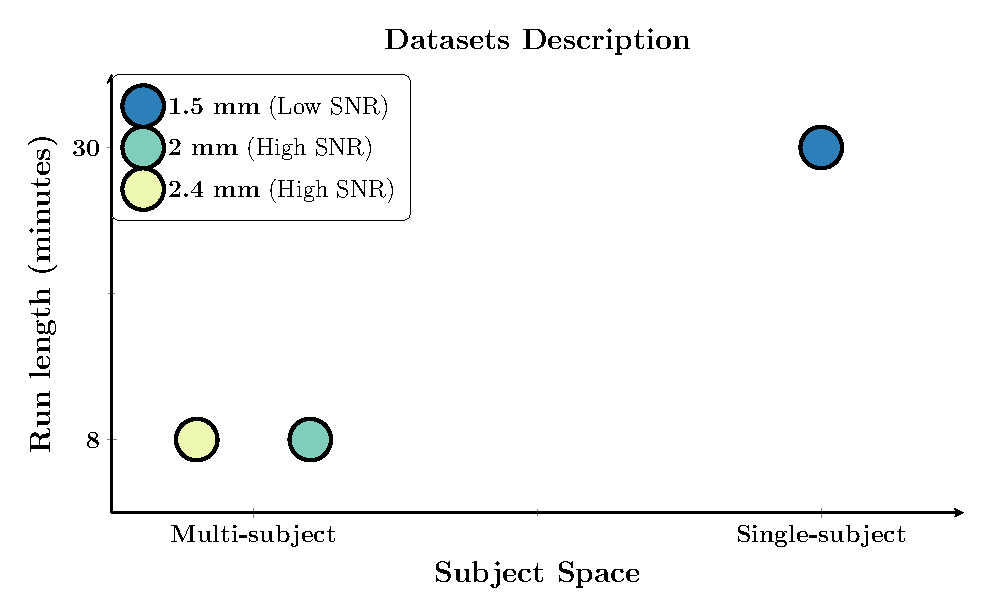
\includegraphics[width=6cm]{images/Datasets.pdf}
     \caption[Resting State datasets overview]{Resting State datasets overview. }
     \label{fig:dataset}
 \end{figure}

\textbf{Multi-echo fMRI datasets:}
\begin{itemize}
\item \textbf{Low resolution (2.4 mm and 2.0 mm) datasets.} Five healthy adult volunteers (three female) were scanned using two distinct four-echo fMRI sequences. For the first sequence, data were acquired with an isotropic voxel size of 2.4 mm (TR = 1.2 s, TEs = 11.2/28.1/45.0/61.9 ms). For the second sequence, data were acquired with an isotropic voxel size of 2.0 mm (TR = 1.7 s, TEs = 13.4/36.1/58.8/81.5 ms). Both sequences employed simultaneous multi-slice (SMS) acceleration with a factor of 5, GRAPPA acceleration with a factor of 2, and, respectively, 65 and 75 whole-head sagittal slices depending on voxel size. The primary objective of these datasets is to characterize the trade-off between temporal and spatial resolution in the context of thermal noise denoising.

\item \textbf{High resolution (1.5 mm) dataset.} A healthy male volunteer was scanned with a three-echo fMRI sequence during two 30-minute runs at 1.5 mm isotropic resolution (TR = 2 s, TEs = 16/46.92/77.84 ms, SMS = 4, partial Fourier (PF) = 6/8, GRAPPA = 2). The primary objective of this dataset is to investigate the impact of denoising at the highest spatial resolution that is practically achievable at 3T, where thermal noise is the dominant contributor to the temporal signal-to-noise ratio (tSNR).
\end{itemize}

\textbf{Thermal denoising.} Each dataset was denoised independently through different algorithms: undenoised (vanilla), mppca, Nordic, Nordic over spatially concatenated echoes (Hydra), or tensor mppca. 

\textbf{Multi-echo fMRI preprocessing.} Multi-echo (ME) fMRI data were minimally preprocessed using AFNI \citep{cox1996afni}. The preprocessing pipeline comprised discarding the initial 10 volumes to ensure steady-state magnetization, realigning the first echo to the single-band reference (SBRef) image, and applying the resulting transformation parameters to all remaining echoes. For the high-resolution dataset, both runs were additionally aligned to the SBRef of the first run using a local Pearson correlation cost function (\texttt{align\_epi\_anat.py}, 3dAllineate). A T2\textbf{*}-weighted optimal linear combination of the echoes was subsequently computed using TEDANA (multi-echo optimal combination, ME-OC). 

To further evaluate the stability of the thermal noise estimation and the associated variance removal in the reliability analysis, the same minimal preprocessing pipeline was independently applied to the first and second halves of the high-resolution dataset time series (see Fig.~\ref{fig:preprocessing}). This additional step was performed exclusively on the high-resolution dataset, as this dataset is expected to exhibit greater noise variance, thereby rendering potential changes more detectable. 

\begin{figure}[htbp]
    \centering
    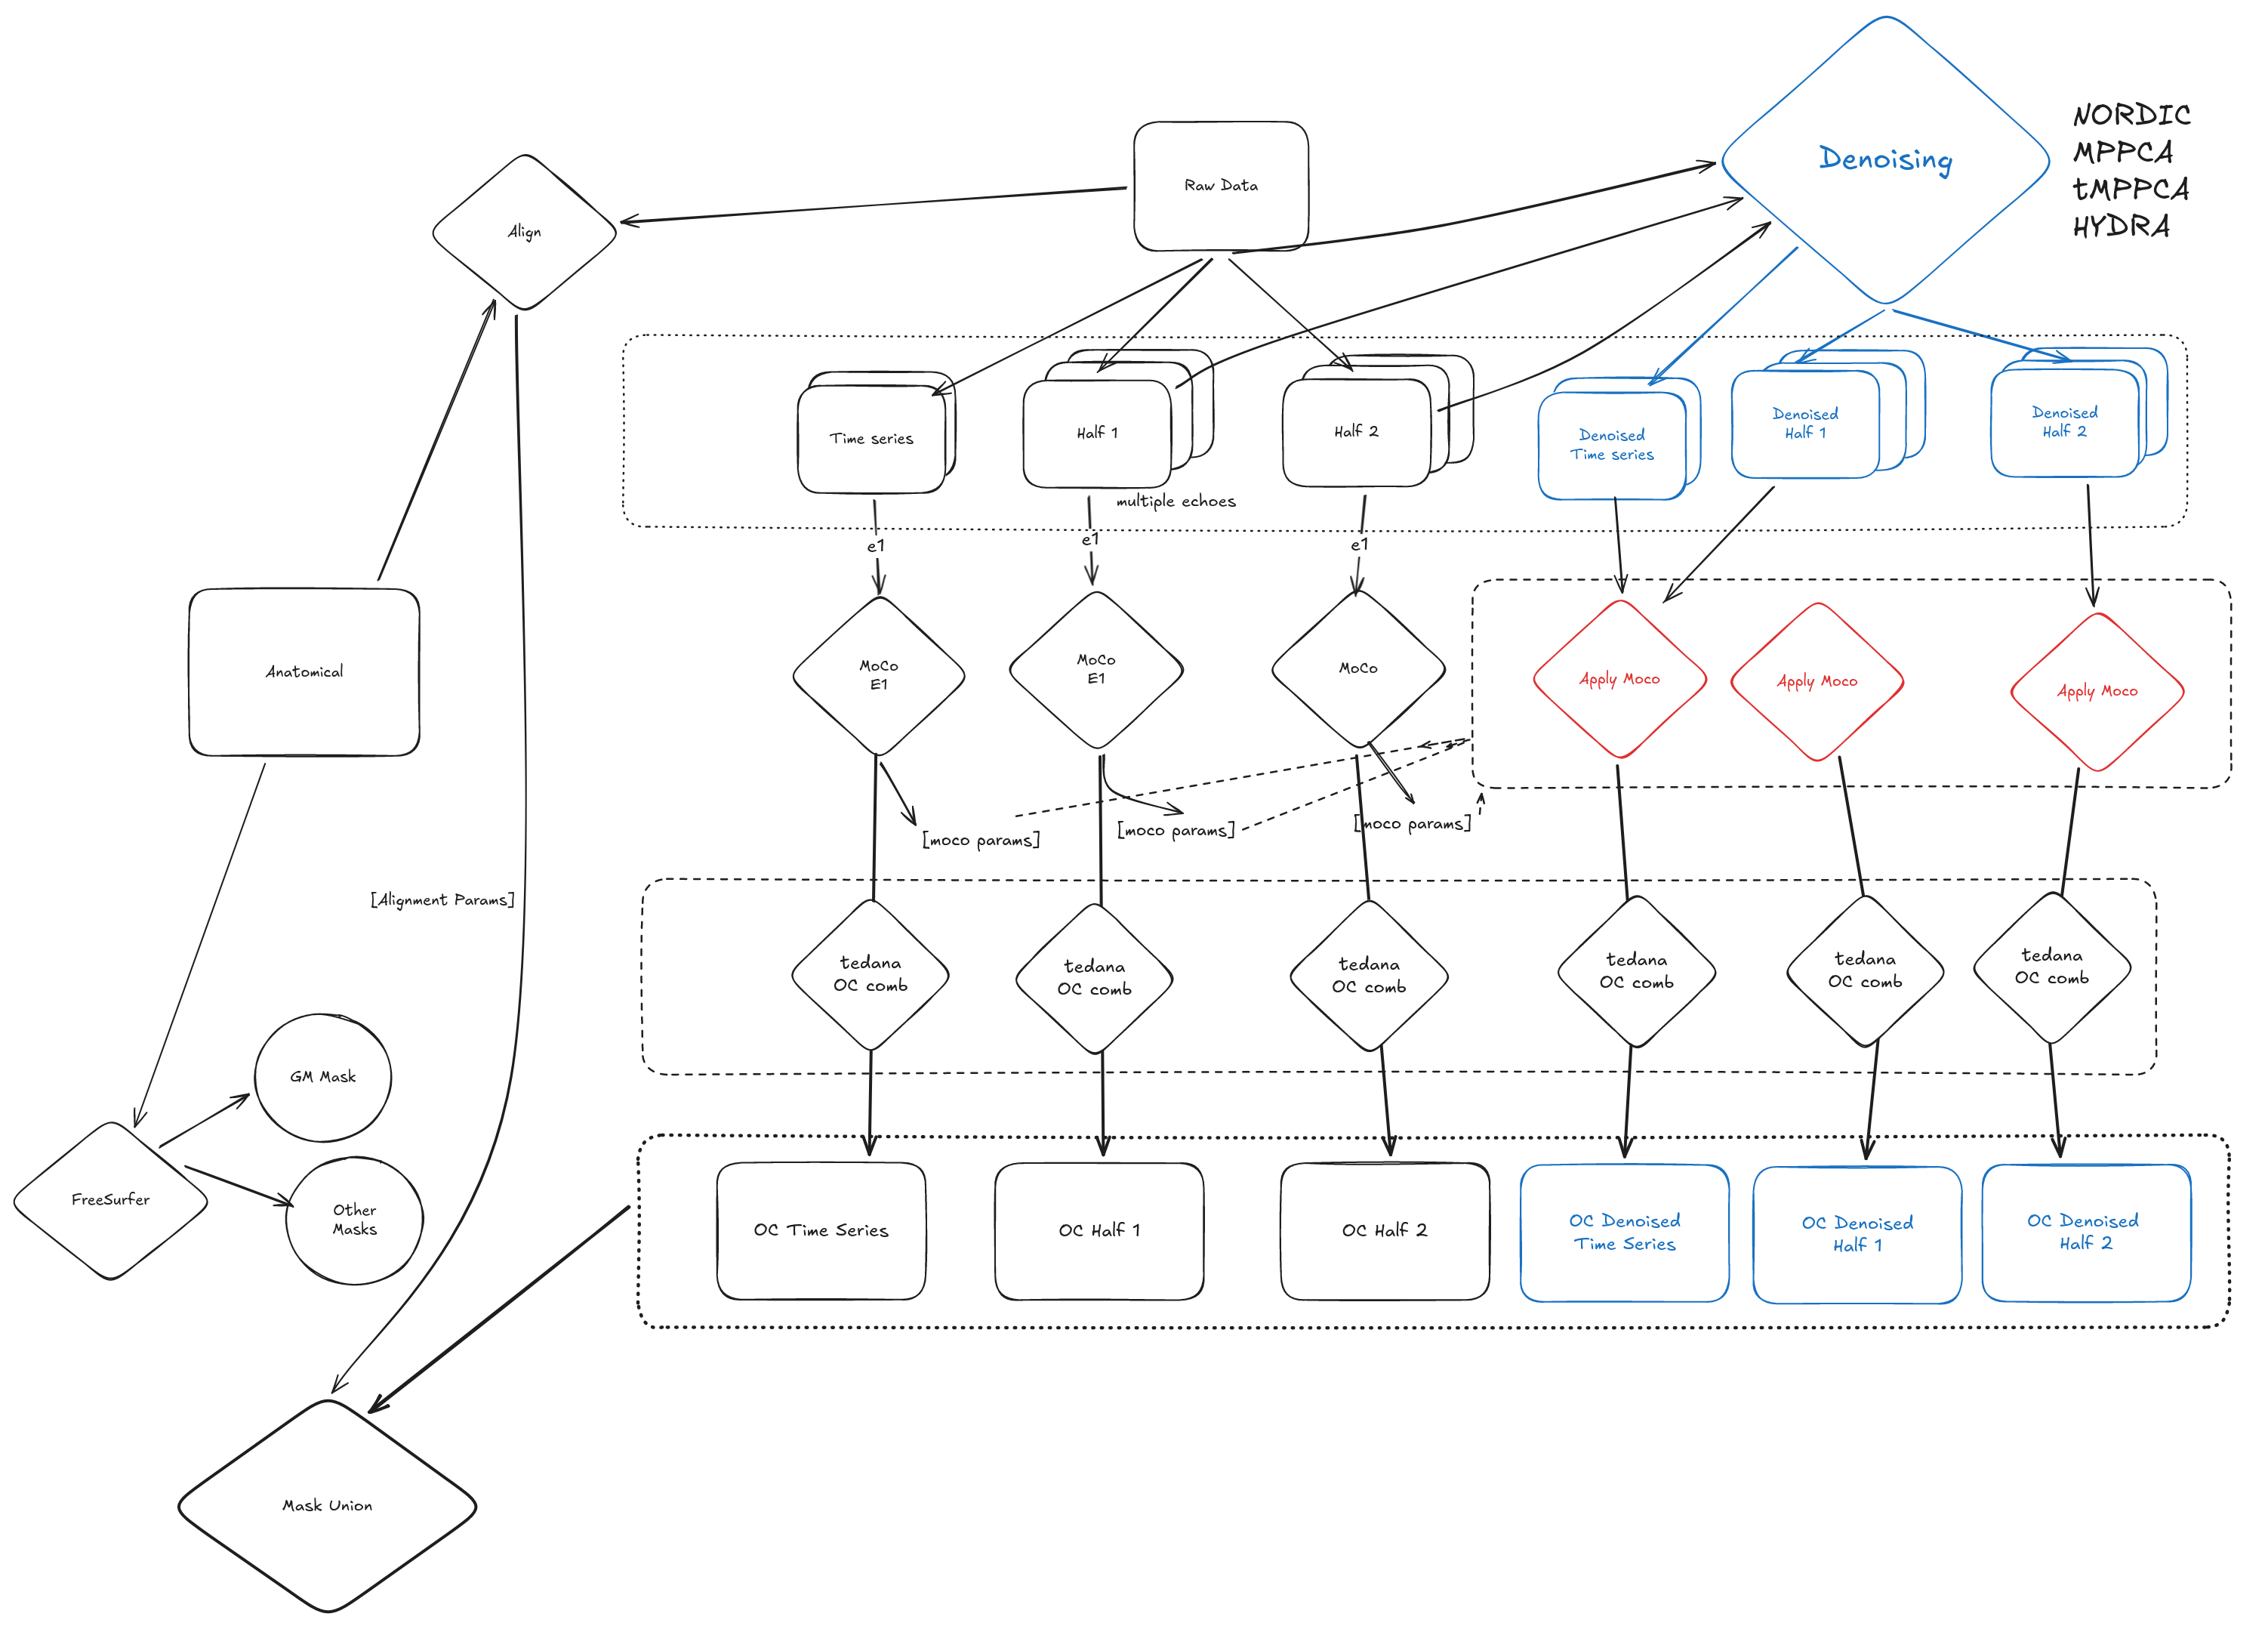
\includegraphics[width=12cm]{images/Process_diagram.png}  
    \caption[Diagram of fMRI preprocessing pipeline.] {For each time series, a minimal preprocessing pipeline was applied, including, for example, motion correction and optimal echo combination. Denoised versions of the same time series underwent an identical preprocessing procedure as the corresponding raw data. The transformation matrix was always derived from the raw time series to prevent potential bias of the rigid-motion parameter estimation by the denoising procedure. Finally, for the reliability analysis, the same minimal preprocessing pipeline was independently applied to the first and second halves of the high-resolution dataset time series to assess the stability of the thermal noise estimation.}
    \label{fig:preprocessing}
\end{figure}

\textbf{Tissue-based region of interests (ROI).} Anatomical images for each dataset were segmented using FreeSurfer (version 7.4.0) with the \texttt{recon-all} pipeline \citep{fischl2004automatically}. The resulting segmentations were subsequently transformed into AFNI volumetric space using the \texttt{@SUMA\_Make\_Spec\_FS} utility. A custom ROI mask was then generated with AFNI’s \texttt{3dcalc}, incorporating the bilateral cortical gray-matter ribbons as well as subcortical structures. From the SUMA output datasets, a skull-stripped anatomical volume was rigid-body aligned to the single-band reference (sbref) image of the first echo. The alignment was estimated using local Pearson correlation as the cost function. The resulting transformation matrix was then applied to the ROI mask to register it from anatomical space into functional space. 


\section{Multi-echo fMRI data analysis}

 In multi‑echo functional magnetic resonance imaging (fMRI), optimal echo combination relies on voxel‑wise estimates of \(S_0\) and \(R_2^* = 1/T_2^*\), obtained via a linear fit across echo times. If thermal denoising effectively attenuates thermal noise variance without altering the underlying BOLD signal, three principal effects are anticipated: (1) an increase in temporal signal‑to‑noise ratio (tSNR); (2) more physiologically plausible time‑varying \(R_2^*\) values, \(\Delta R_2^*\); and (3) enhanced test‑retest reliability of functional connectivity (FC) matrices, while preserving unbiased estimates of the core parameters \(S_0\) and \(T_2^*\). Accordingly, we quantify the performance of each denoising approach by characterizing its impact on \(S_0\), \(R_2^*\), \(\Delta R_2^*\), tSNR, and FC reliability.
 
\begin{itemize}
\item\textbf{Temporal Signal-to-Noise Ratio (tSNR):} tSNR maps were computed from the whole-brain ME-OC time series to characterize data quality after denoising. This metric reflects the noise regime of the data and thereby constrains the sensitivity to detect activity-related signal fluctuations. Given that BOLD signal changes are typically small in magnitude (see Sec.~\ref{sec:BOLD}), higher tSNR values are desirable. tSNR was defined as
\begin{equation}
    tSNR = \frac{\overline{S}}{\sigma_S},
\end{equation}
where $\overline{S}$ denotes the temporal mean signal intensity and $\sigma_S$ its temporal standard deviation. Following \citet{liu2016noise}, we expect tSNR values to increase proportionally to the extent to which a denoising method reduces variance. Consequently, denoising strategies yielding higher tSNR values are interpreted as providing higher signal quality, primarily through the reduction of thermal noise variance.

To quantify the magnitude of tSNR changes across denoising methods, we used the vanilla preprocessing pipeline as the baseline. We then computed the percentage change in tSNR, $\Delta tSNR$ (see Fig.~\ref{fig:tsnrDistributionspc}), as the relative difference between a given denoising method and vanilla according to
\begin{equation}
\Delta tSNR = \frac{tSNR_{\mathrm{method}} - tSNR_{\mathrm{vanilla}}}{tSNR_{\mathrm{vanilla}}}.
\end{equation}


\item\textbf{Estimation of Transverse relaxation rate ($R_{2}^*$) and net magnetization ($S_0$):} Estimates of the effective mean transverse relaxation rate, $R_{2}^{*}=1/T_2^*$, and the mean net magnetization, $S_0$, were derived from exponential decay time-series obtained using the \texttt{t2smap} script in \texttt{tedana} \citep{dupre2021te, kundu2012differentiating}. These estimates were computed at each time point after independently fitting a signal model across echoes (option -fitmode='ts'). This procedure yields two 4D datasets (i.e., space + time) in which each volume represents the spatial distribution of the $R_{2}^{*}$ and $S_0$ parameters at a given time point. For each voxel, we subsequently calculated the average relaxation rate $\overline{R_2^*}$ and average net magnetization $S_0$ as an approximation of the underlying (true) relaxation rate. Similar to the tSNR analysis, we computed $\Delta \overline{R_2^*}$ and $\Delta S_0$ maps to assess the changes with respect to the original values without denoising (i.e. relative to vanilla) as follows:
\begin{equation}
\Delta  \overline{R_{2}^*}_\mathrm{method}= \frac{ \overline{R_{2}^*}_\mathrm{method} - \overline{R_{2}^*}_\mathrm{vanilla}}{\overline{R_{2}^*}_\mathrm{vanilla}}, 
\end{equation}

and

\begin{equation}
\Delta S_{0,\mathrm{method}} = \frac{S_{0,\mathrm{method}} - S_{0,\mathrm{method}}}{S_{0,\mathrm{vanilla}}}.
\end{equation}

In addition, we also computed the deviation of the instantaneous relaxation rate estimates from its average value, i.e. , $\Delta R_2^*(t) = R_2^*(t) - \overline{R_2^*}$, expressed in units of s$^{-1}$. We assumed that physiologically driven fluctuations in relaxation rate occur within a range of approximately $|1 \text{ s}^{-1}|$ \citep{vanderzwaagFMRI1532009, caballerogaudesParadigmFreeMapping2011}; thus, we examined how thermal denoising influenced the physiological plausibility of instantaneous $\Delta R_2^*$ signal changes (see Fig.~\ref{fig:plausabilityR2}).



\item\textbf{Functional Connectivity Reliability:} Reliability maps were calculated following the procedures described in \citet{lynchRapidPrecisionFunctional2020} (see Fig.~\ref{fig:FCreliability}). Specifically, for each ME-OC timeseries, FC maps were created using each gray matter (GM) voxel as a seed by computing  the Pearson's linear correlation between the seed timeseries and the timeseries of the rest of GM voxels. This results in a FC matrix with $voxel\times voxel$ dimension. FC maps were calculated independently for the first and second half of each timeseries, and voxelwise reliability was calculated as the linear correlation ($r^{2}$) between the FC values obtained in the first half of the acquisition, here considered as ground truth, and the FC values of the second half of the acquisition. Reliability values indicate similarity between the FC of a given voxel between both halves, therefore we use as a way to test signal stability through time. $\Delta r^2$ maps to assess the changes with respect to the original values without denoising (i.e. relative to vanilla) were computed as follows:
\begin{equation}
\Delta   r^2_\mathrm{method}= \frac{  r^2_\mathrm{method} -  r^2_\mathrm{vanilla}}{ r^2_\mathrm{vanilla}}, 
\end{equation}

This procedure was applied to all datasets: the original dataset without denoising (i.e. vanilla) and after denoising with each of the evaluated approaches considering their entire duration. In addition, the longer acquisition of the 1.5 mm dataset (one run of 30 min) allowed us to apply thermal denoising in segments of 15 min duration independently, which is consistent with typical scan lengths in current research resting state studies and compared against the FC reliability between halves of the full 30‑min run.The underlying assumption is that if denoising consistently estimates the noise floor, then independent denoising of shorter segments should yield reliability scores similar to those obtained from joint denoising of the full run. Any systematic deviation would indicate that the effectiveness of noise suppression depends on scan duration.


\end{itemize}

\label{sec:methodsRS}

\section{Results}
\sectionmark{Results}
\label{sec:ResultsRS}
%%%%%%-------
% -----------tSNR
% -----------
%%%%%%-------
\subsection{Temporal Signal-to-Noise Ratio (tSNR)}
%%%%%  -- 2.4 mm -- %%%%%
%-- boxplots
\begin{figure}[htbp]
\centering \colorbox{white}{
    \centering
    \begin{tabular}{>{\centering\arraybackslash}m{.7cm}>{\centering\arraybackslash}m{9cm}}
       & \textcolor{black}{\textbf{$tSNR$}}  \\
    \rotatebox[origin=l]{90}{\textcolor{black}{2.4 mm}} &    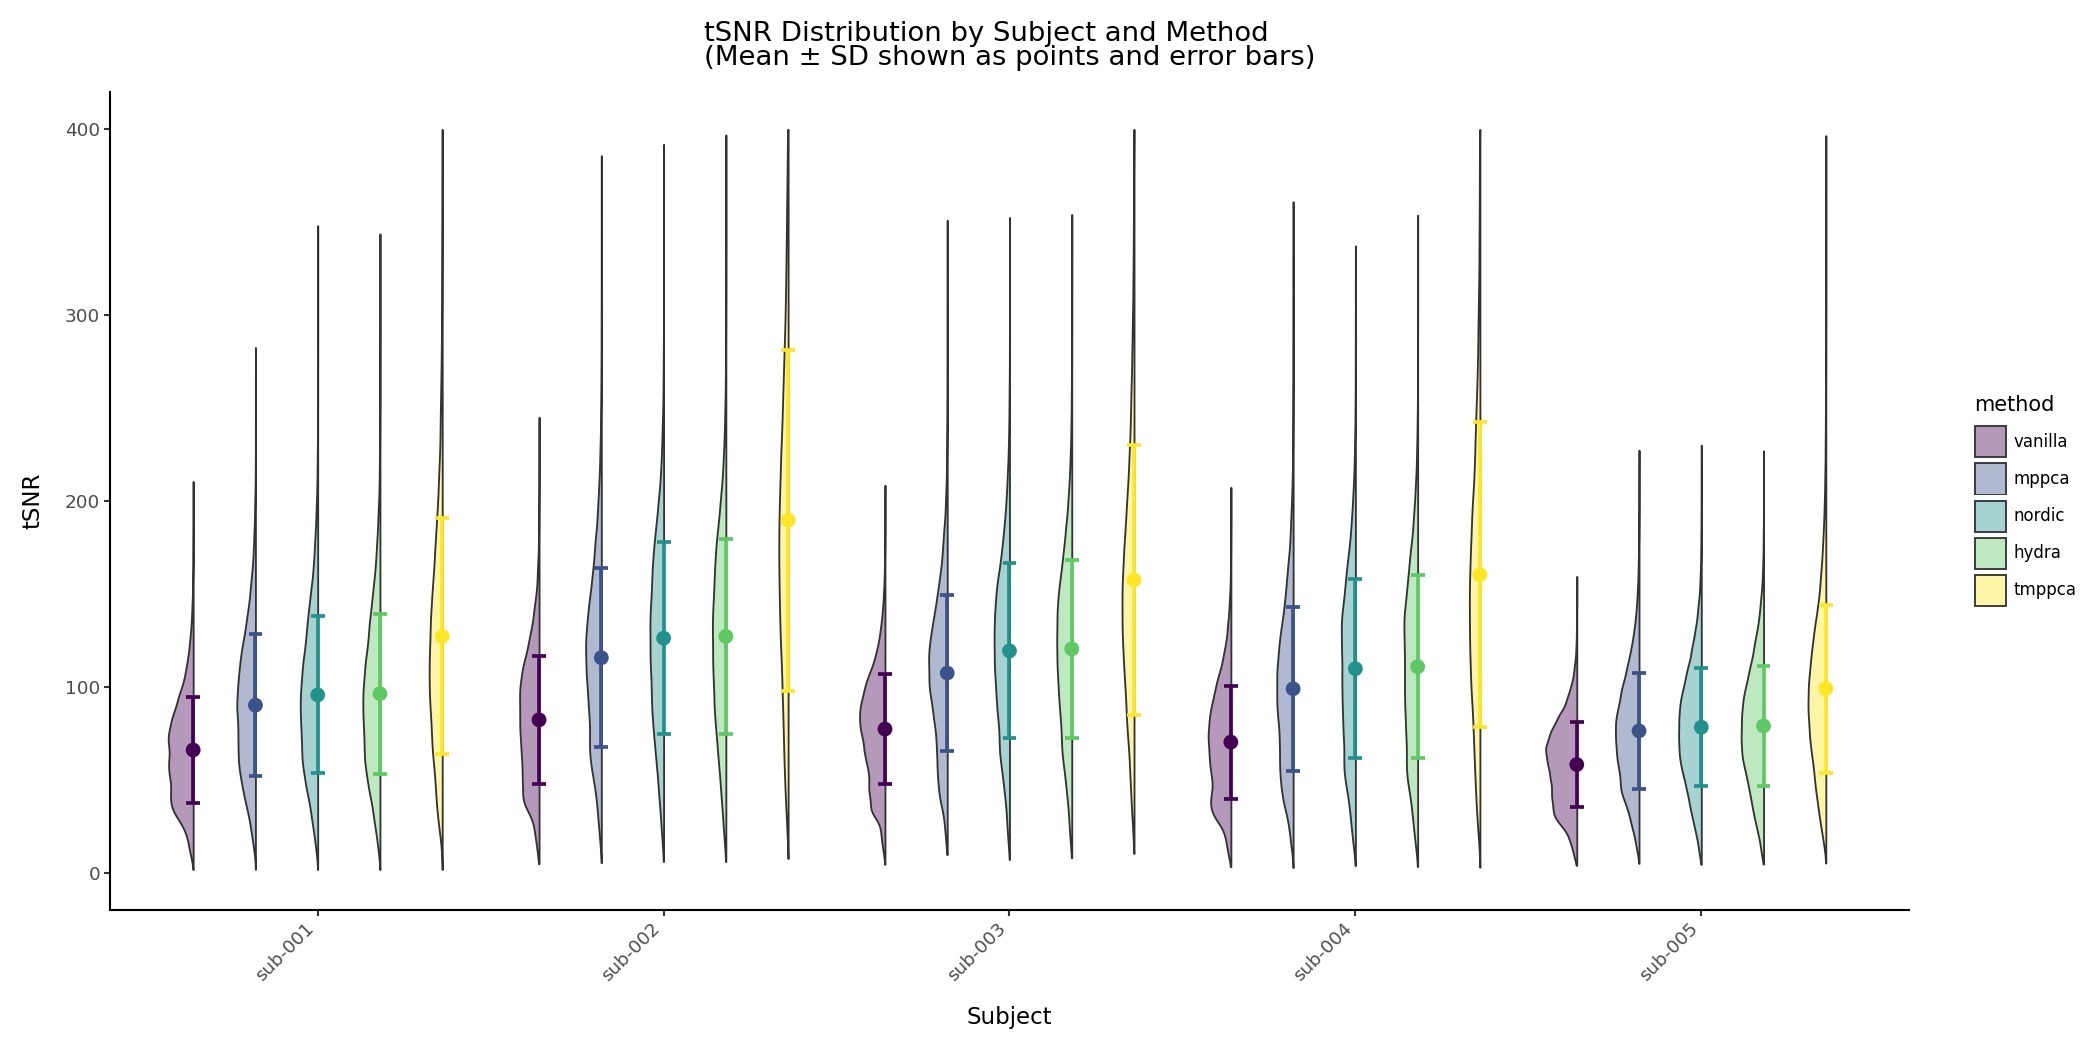
\includegraphics[width=9cm]{images/halfviolin_tsnr_across_subjects_masked1200.png} \\
       \rotatebox[origin=l]{90}{\textcolor{black}{2 mm}} & 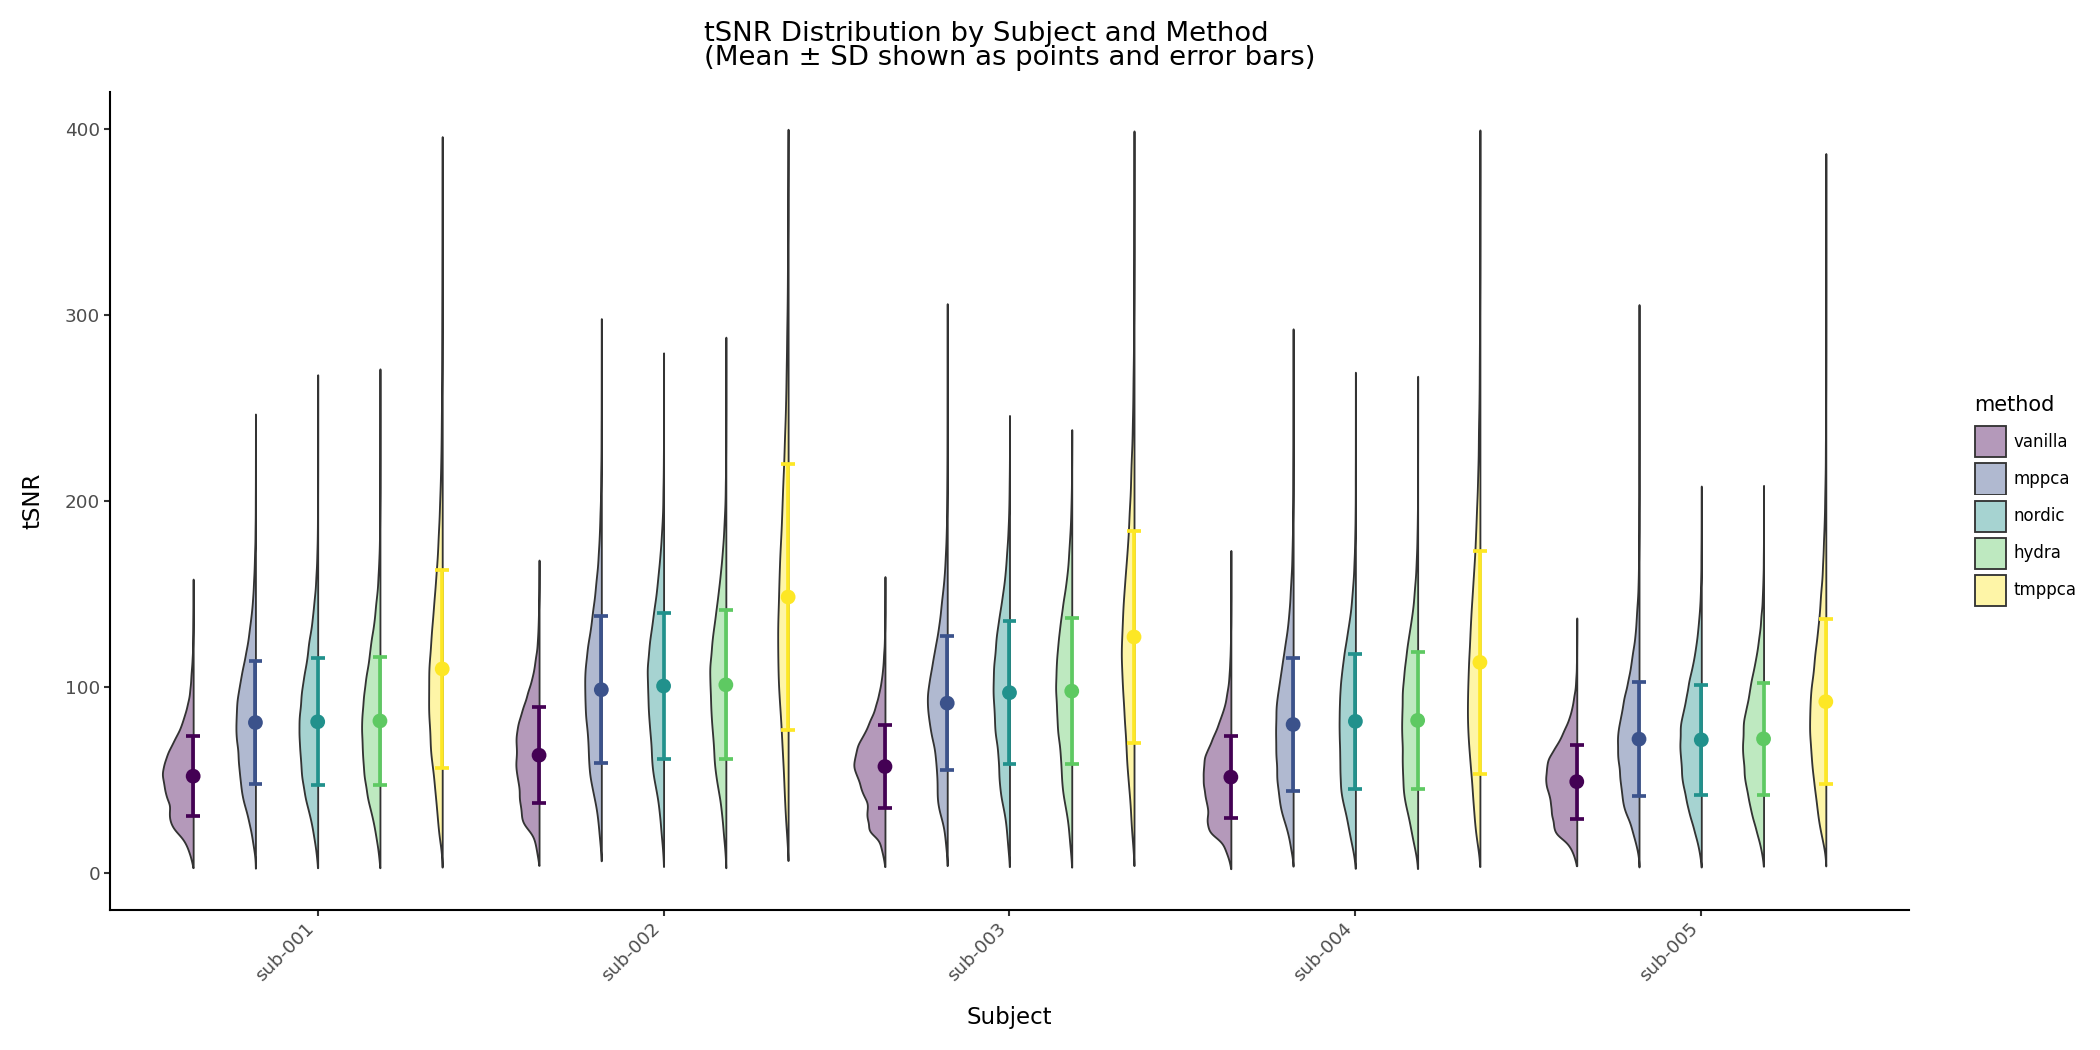
\includegraphics[width=9cm]{images/halfviolin_tsnr_across_subjects_masked1700.png} \\
      \rotatebox[origin=l]{90}{\textcolor{black}{1.5 mm}}&   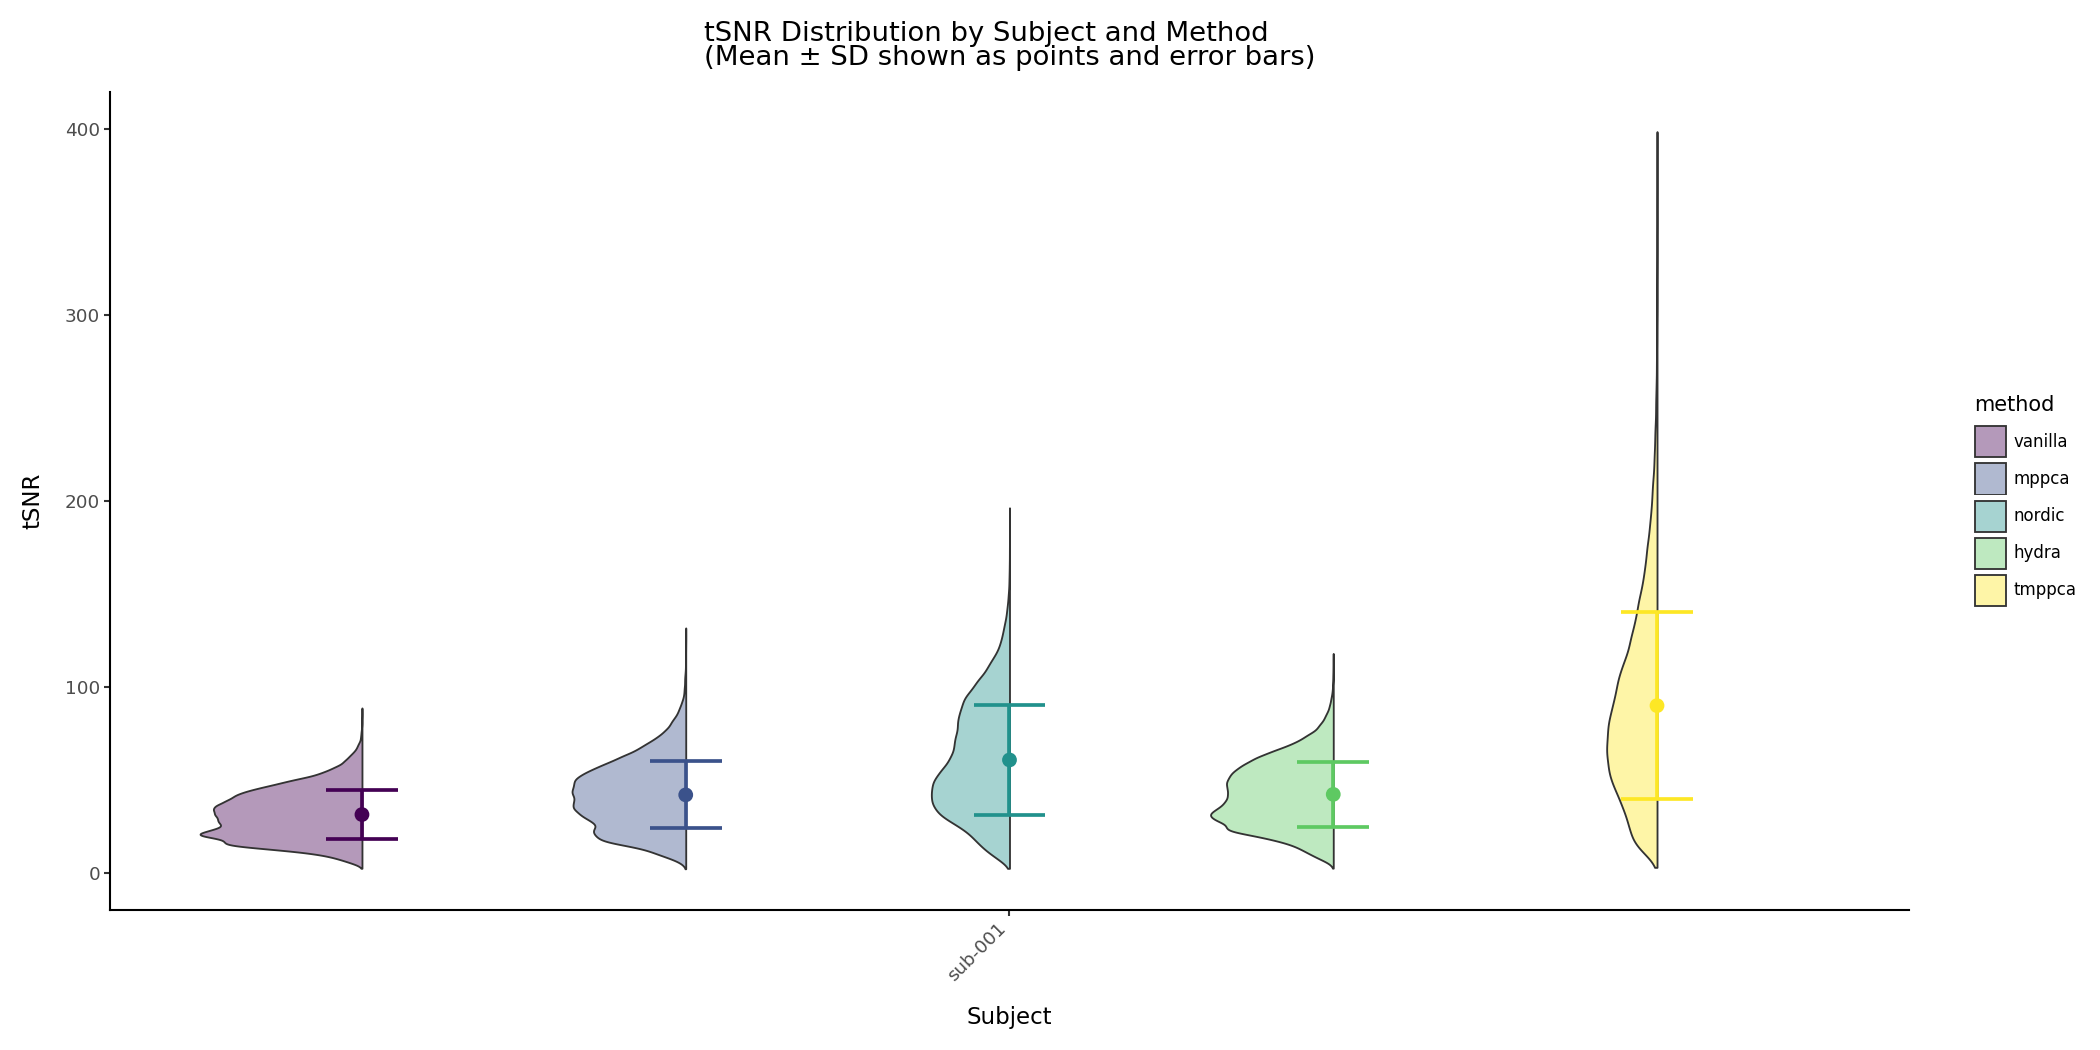
\includegraphics[width=9cm]{images/halfviolin_tsnr_across_subjects_maskedHR.png}    \\
    \end{tabular}
    }
    \caption[Distribution of tSNR values per dataset]{Violin plots of tSNR per method and resolution.}
    \label{fig:tsnrDistribution}
\end{figure}

\begin{figure}[htbp]
\centering \colorbox{white}{
    \centering
    \begin{tabular}{>{\centering\arraybackslash}m{.7cm}>{\centering\arraybackslash}m{9cm}}
       &  \textcolor{black}{\textbf{$\Delta  \ tSNR$}} \\
    \rotatebox[origin=l]{90}{\textcolor{black}{2.4 mm}} &
        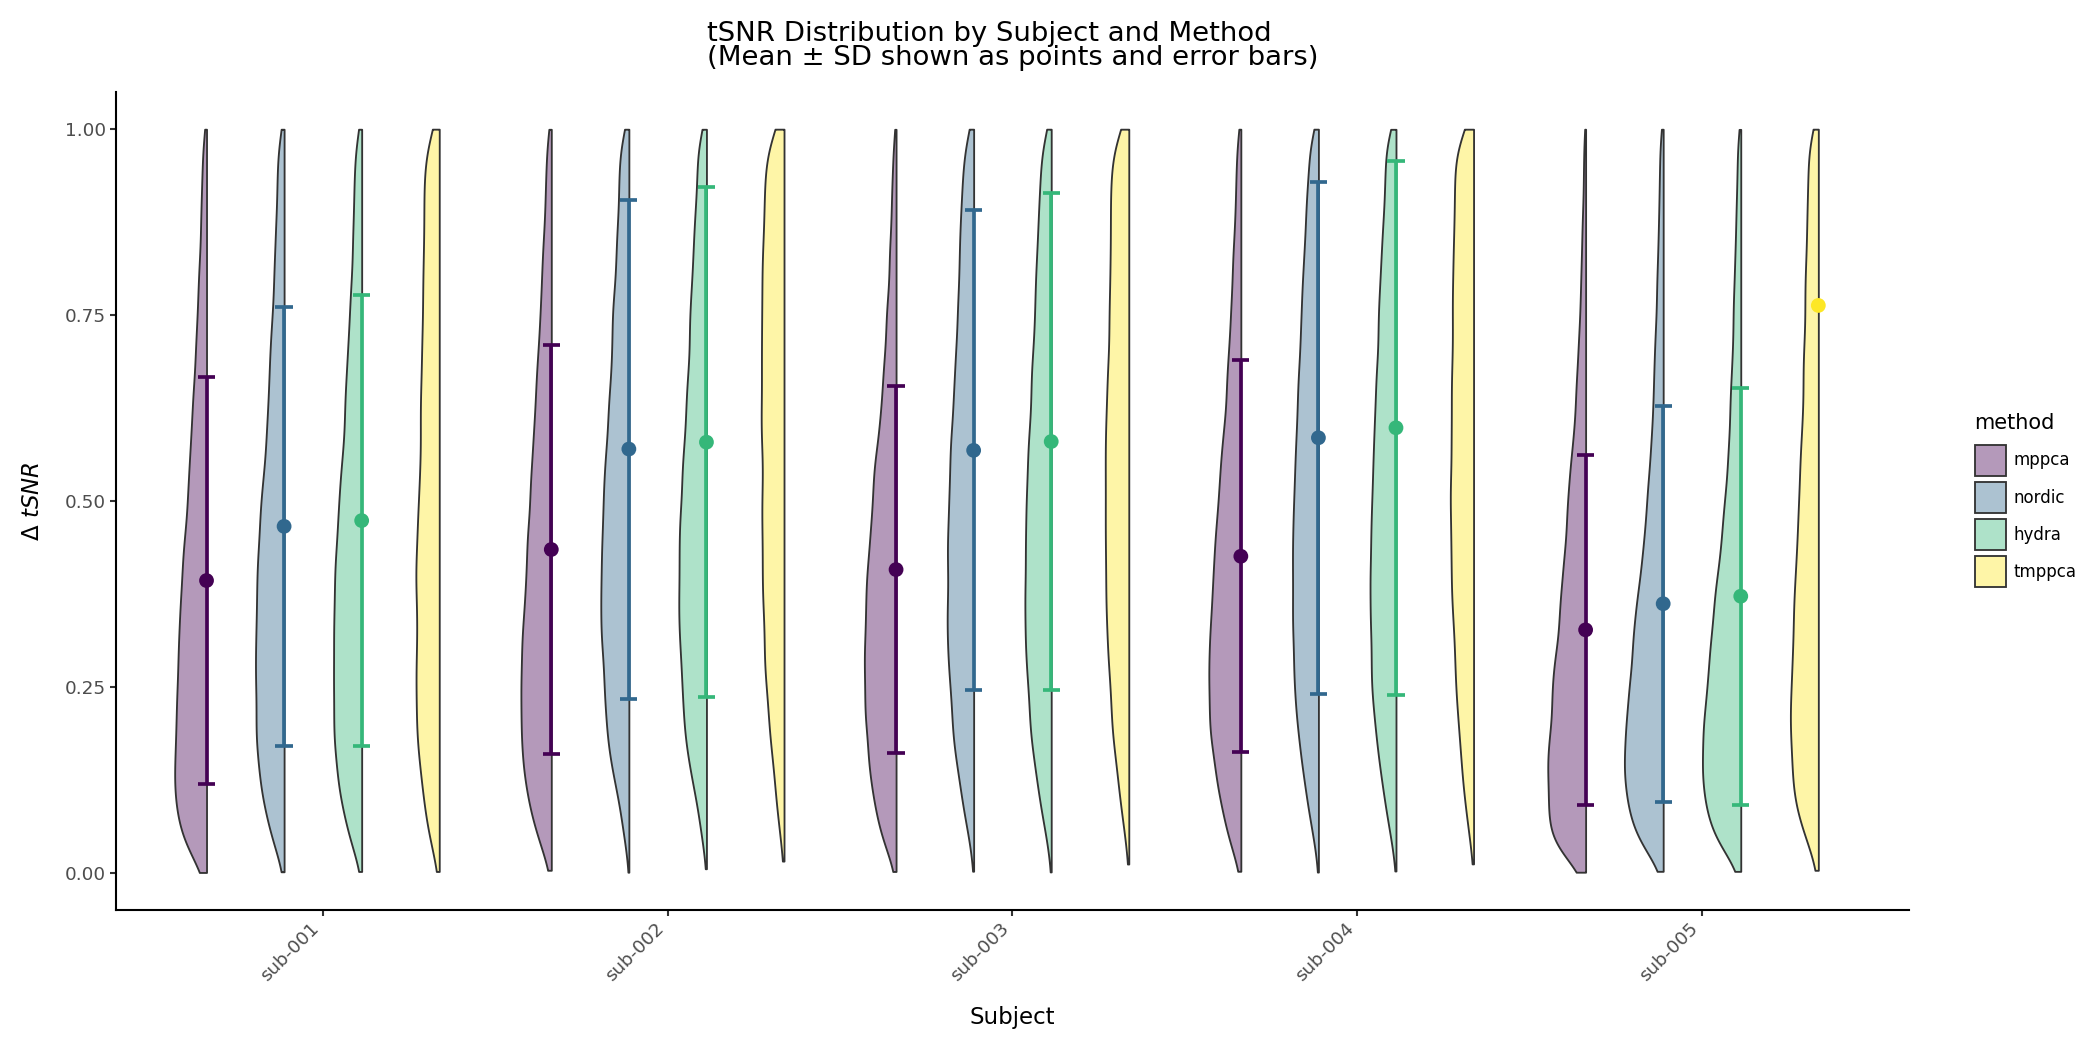
\includegraphics[width=9cm]{images/halfviolin_tsnrspc_across_subjects_masked1200.png}\\
       \rotatebox[origin=l]{90}{\textcolor{black}{2 mm}}&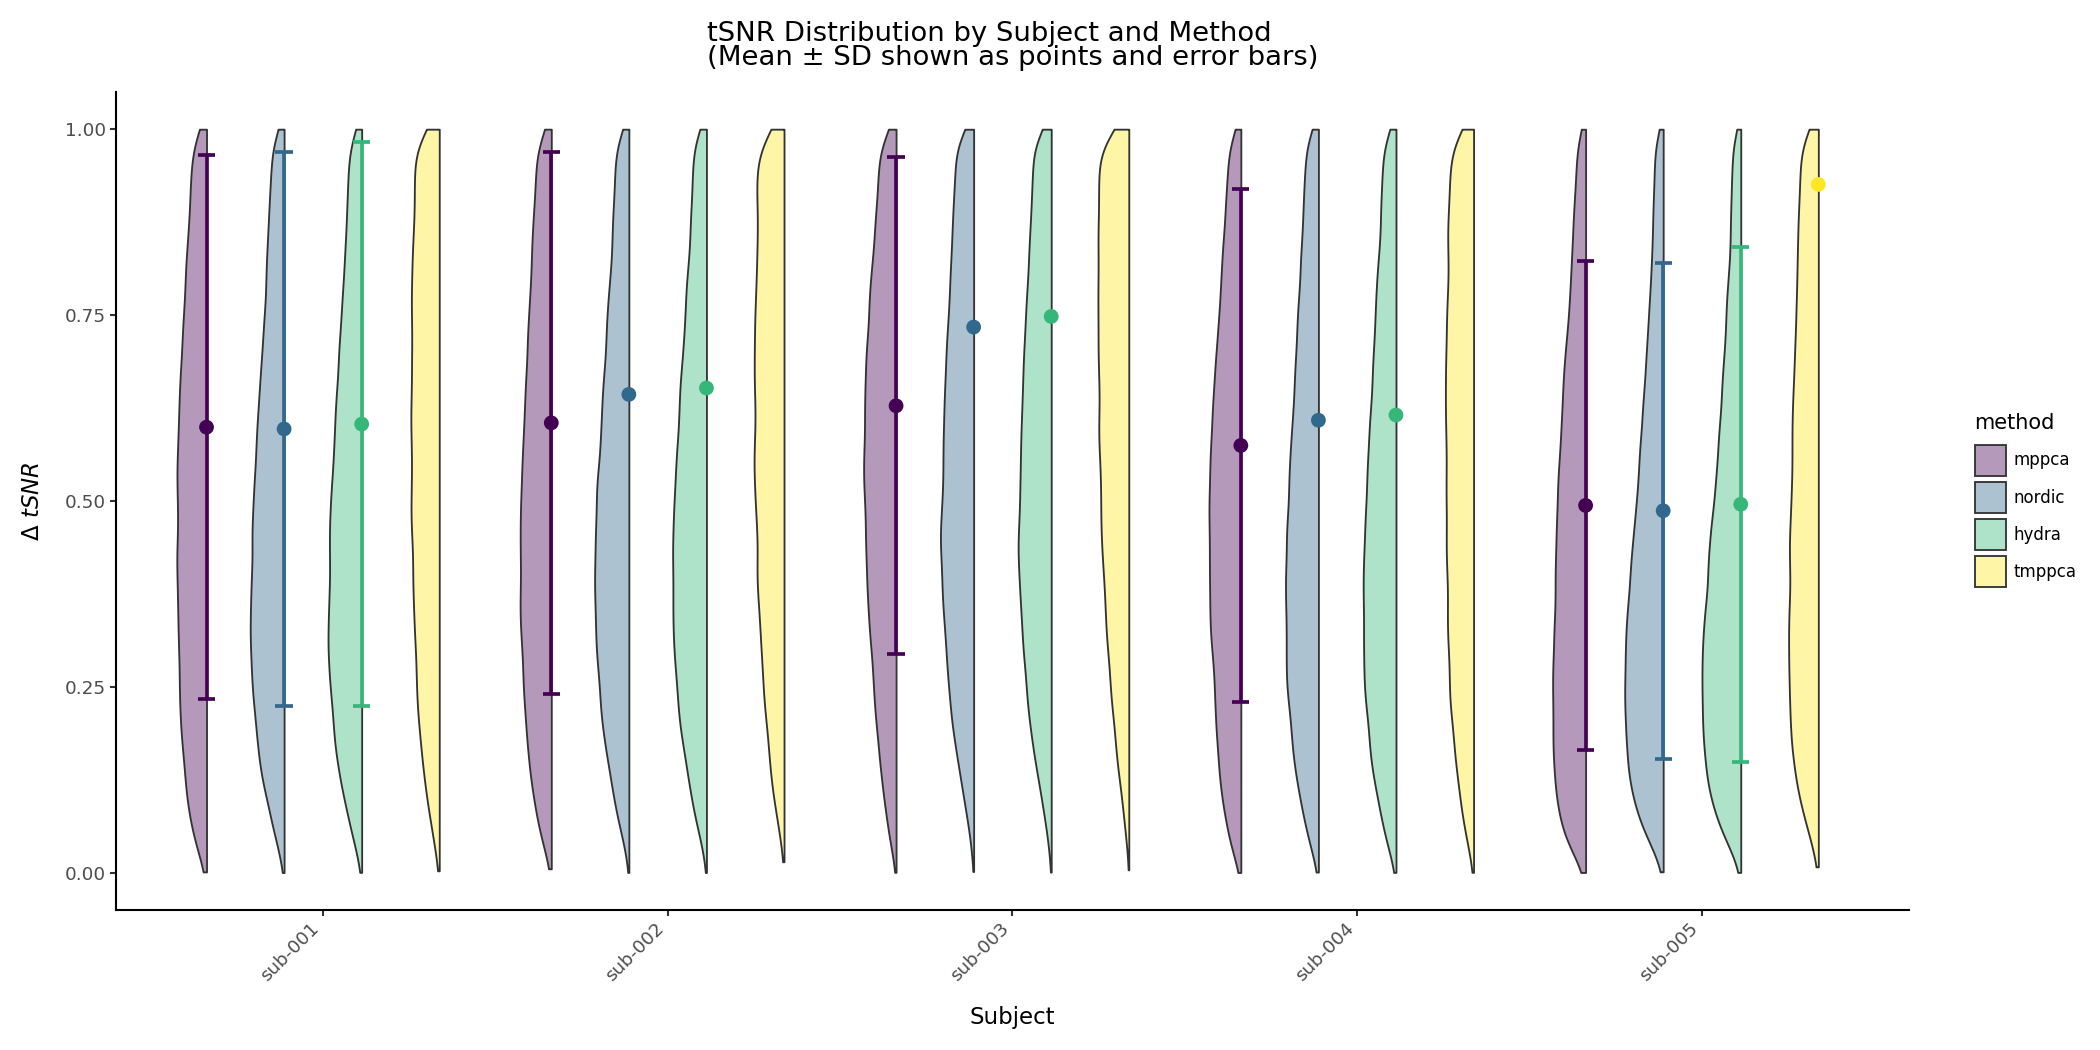
\includegraphics[width=9cm]{images/halfviolin_tsnrspc_across_subjects_masked1700.png} \\
      \rotatebox[origin=l]{90}{\textcolor{black}{1.5 mm}}   &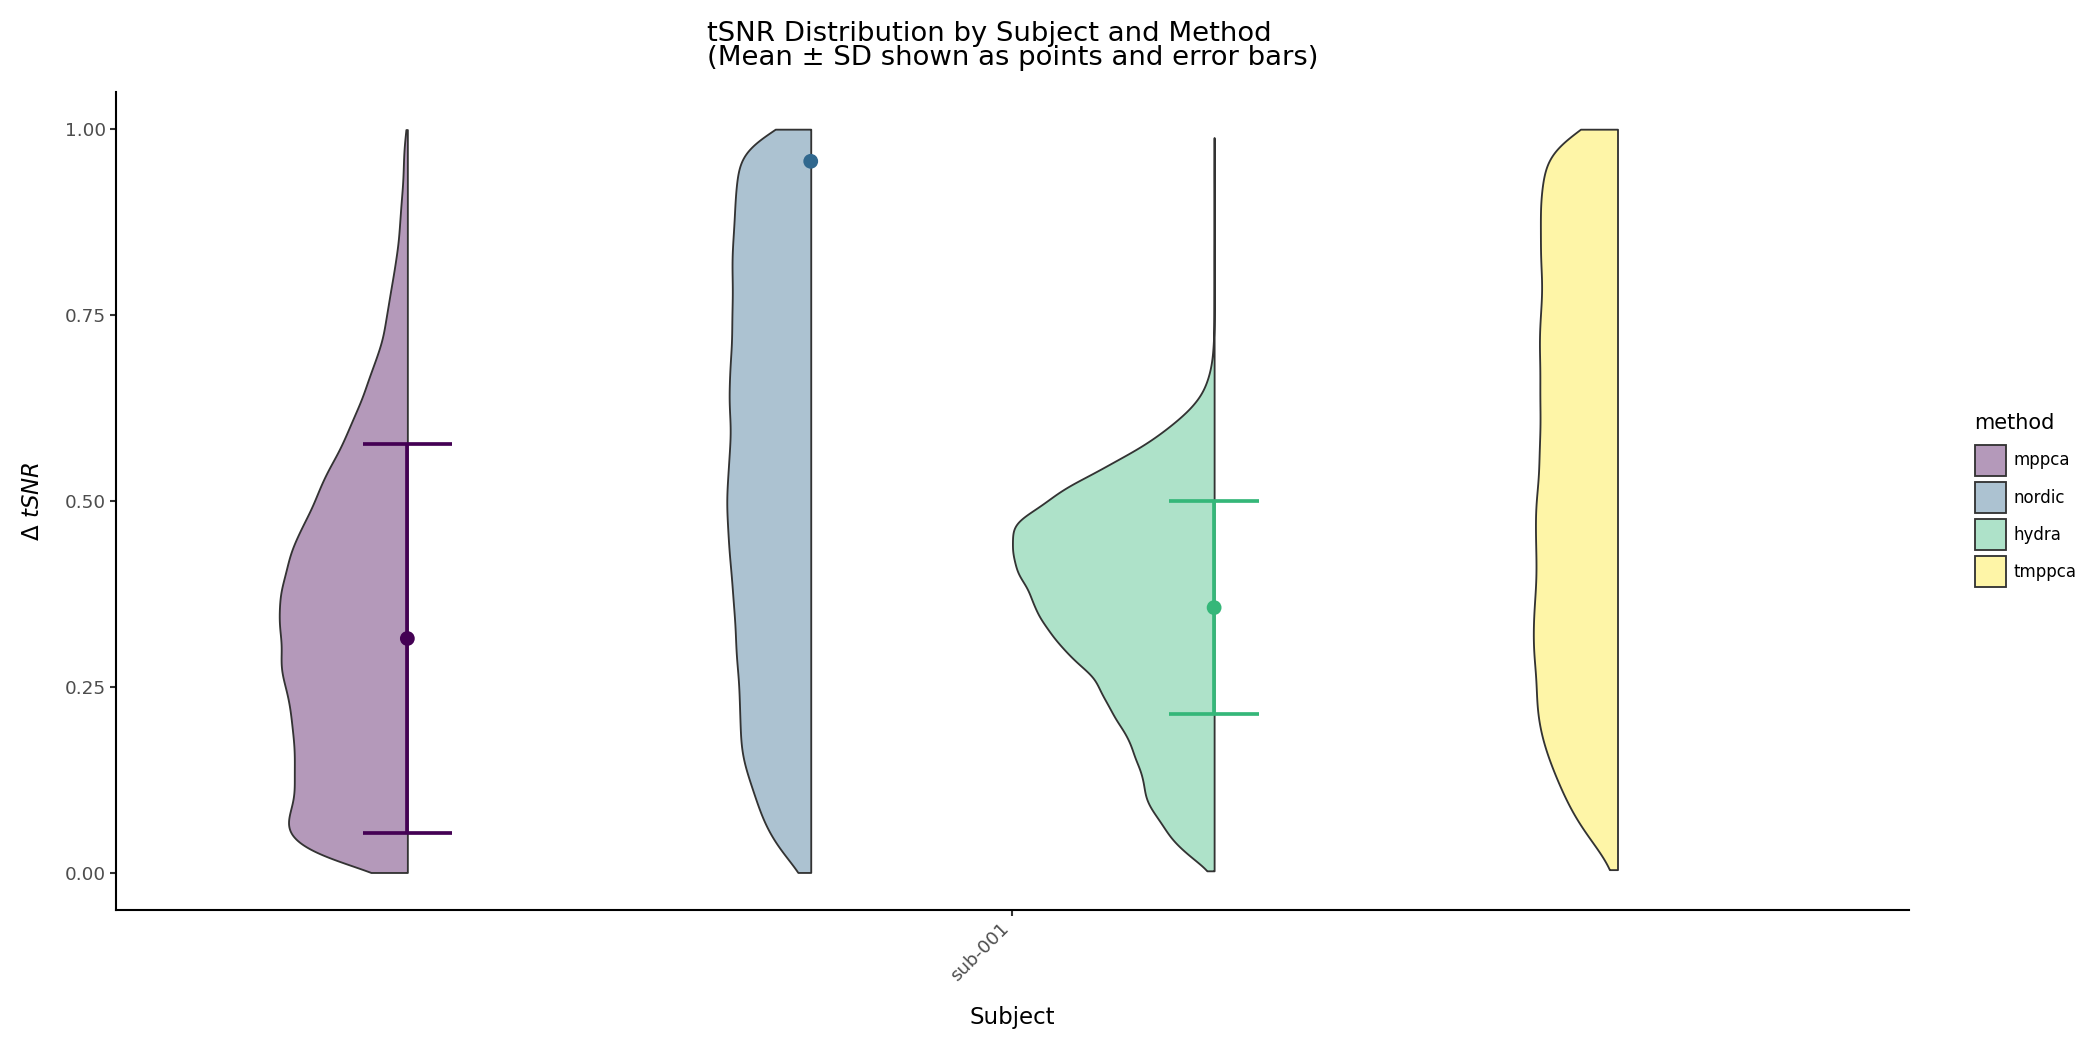
\includegraphics[width=9cm]{images/halfviolin_tsnr_across_subjects_masked.png} \\
    \end{tabular}
    }
    \caption[Distribution of changes in tSNR values per dataset]{Violin plots of  $\Delta$tSNR (change relative to vanilla)  per method and resolution}
    \label{fig:tsnrDistributionspc}
\end{figure}


As expected, the tSNR maps revealed an inverse relationship with spatial resolution, with lower resolution datasets exhibiting higher tSNR values ($2.4\text{mm} > 2\text{mm} > 1.5\text{mm}$), as illustrated in Fig.~\ref{fig:tsnrDistribution}. A voxel-wise analysis of the relative change in temporal signal-to-noise ratio ($\Delta t\text{SNR}$) across all participants demonstrated that, among the denoising strategies evaluated, TMPPCA consistently yielded the greatest increase in tSNR relative to the vanilla (non-denoised) condition. Although all denoising methods reduced data variance, a consistent hierarchy in tSNR values was observed: TMPPCA $>$ NORDIC $>$ MPPCA $>$ VANILLA. Notably, HYDRA exhibited performance comparable to NORDIC in the low-resolution datasets, whereas in the high-resolution dataset its performance was similar to that of MPPCA. However, this analysis alone cannot determine whether the reduction in variance translates into improved data quality, i.e., it corresponds to noise removal or if it comes along with the attenuation of the signal of interest.

\subsubsection{tSNR analysis: low resolution Datasets (2.4 mm \&  2 mm)}

\begin{figure}[htbp]
\centering \colorbox{black}{
    \centering
    \begin{tabular}{>{\centering\arraybackslash}m{.7cm}>{\centering\arraybackslash}m{3cm}>{\centering\arraybackslash}m{3cm}>{\centering\arraybackslash}m{.7cm}}
    
       & \textcolor{white}{\textbf{tSNR}} & \textcolor{white}{\textbf{$\Delta tSNR$}}& \\
   \rotatebox[origin=l]{90}{\textcolor{white}{VANILLA}}
  &    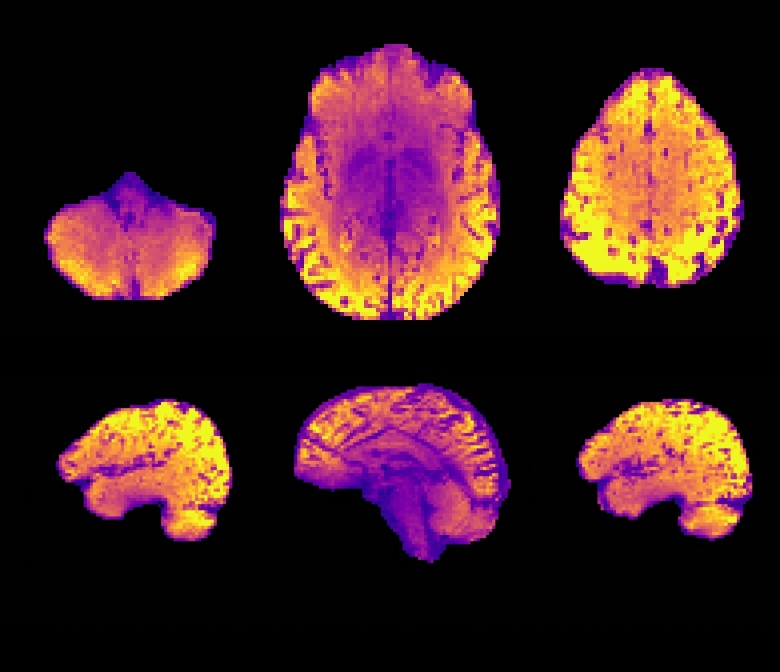
\includegraphics[width=3cm]{images/sub-001_ses-1_task-HABLA1200_OC_part-mag_bold_vanilla_tsnr_all.jpg} & & \textcolor{white}{tSNR} 
\includegraphics[width=.5cm]{images/Plasmatsnr.png}\\
     \rotatebox[origin=l]{90}{\textcolor{white}{MPPCA}}
  &    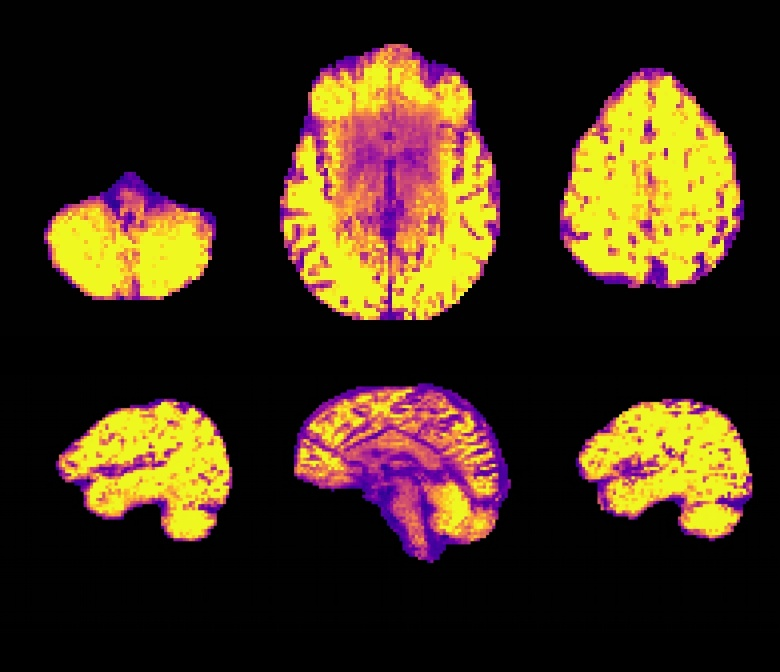
\includegraphics[width=3cm]{images/sub-001_ses-1_task-HABLA1200_OC_part-mag_bold_mppca_tsnr_all} &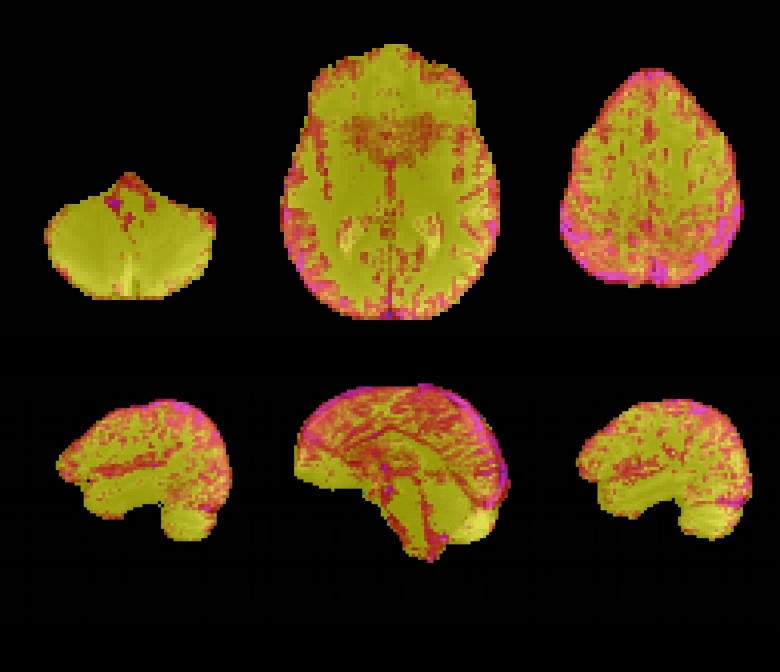
\includegraphics[width=3cm]{images/sub-001_ses-1_task-HABLA1200_OCspc_part-mag_bold_mppca_all} &\\
       \rotatebox[origin=l]{90}{\textcolor{white}{NORDIC}}
  &    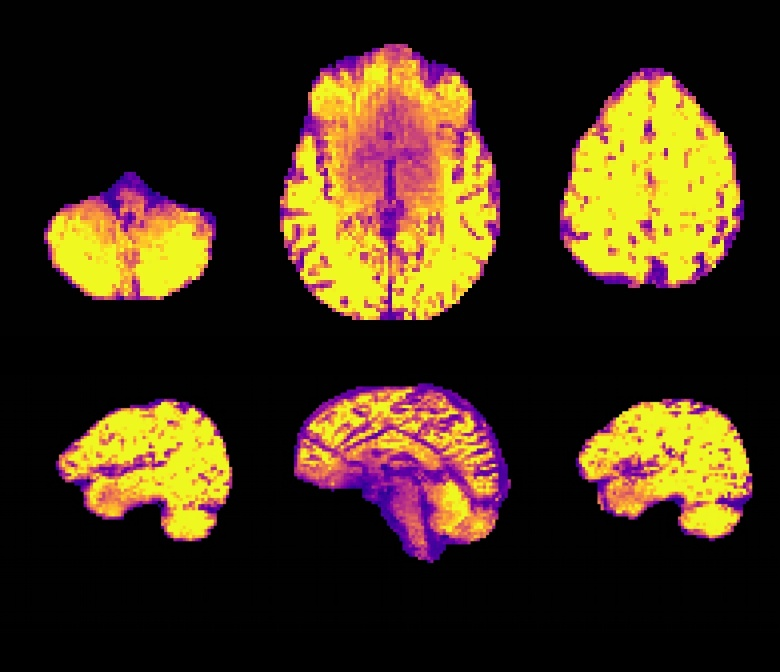
\includegraphics[width=3cm]{images/sub-001_ses-1_task-HABLA1200_OC_part-mag_bold_nordic_tsnr_all.jpg} &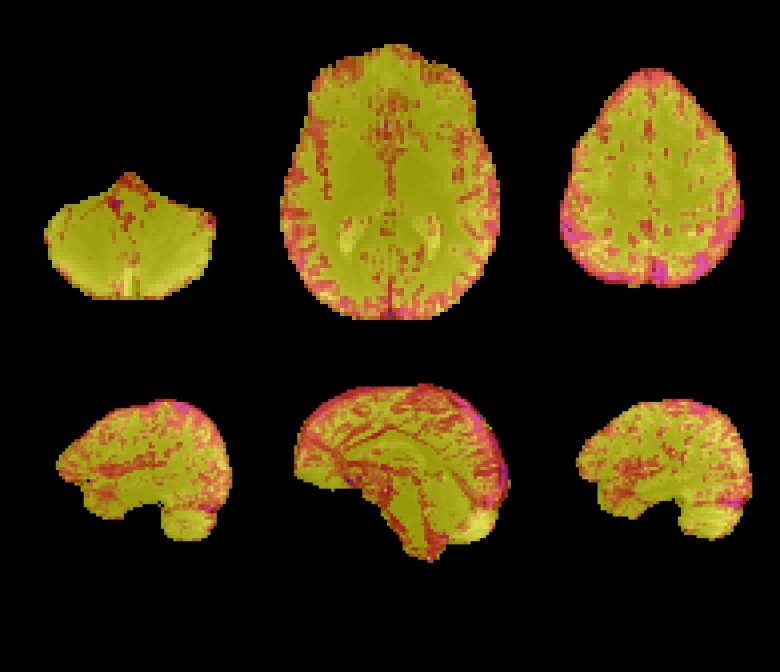
\includegraphics[width=3cm]{images/sub-001_ses-1_task-HABLA1200_OCspc_part-mag_bold_nordic_all} &\\
       \rotatebox[origin=l]{90}{\textcolor{white}{HYDRA}}
  &    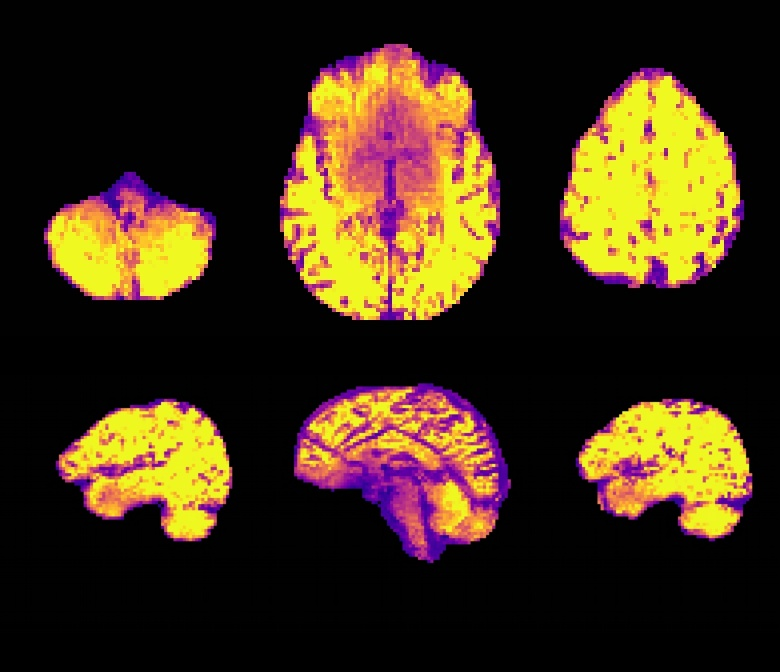
\includegraphics[width=3cm]{images/sub-001_ses-1_task-HABLA1200_OC_part-mag_bold_hydra_tsnr_all.jpg} &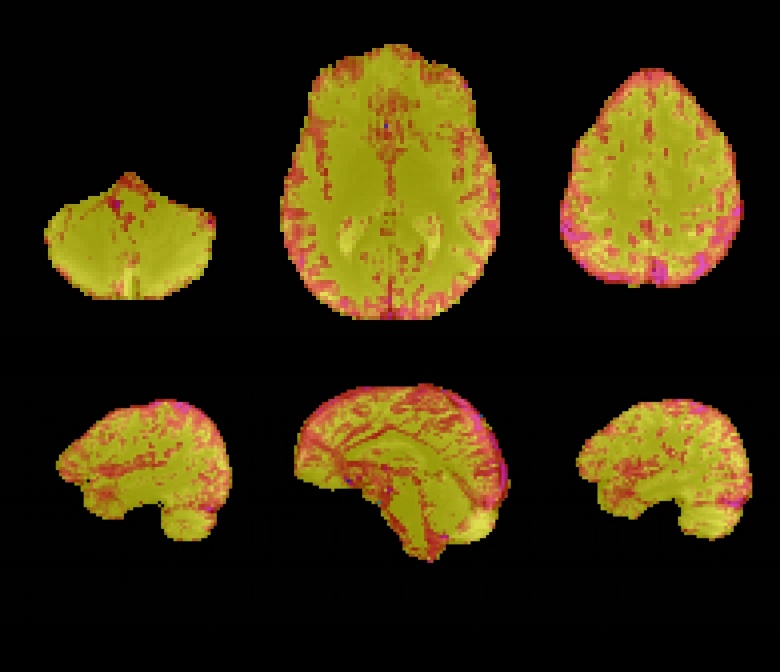
\includegraphics[width=3cm]{images/sub-001_ses-1_task-HABLA1200_OCspc_part-mag_bold_hydra_all} &\\
       \rotatebox[origin=l]{90}{\textcolor{white}{TMPPCA}}
  &    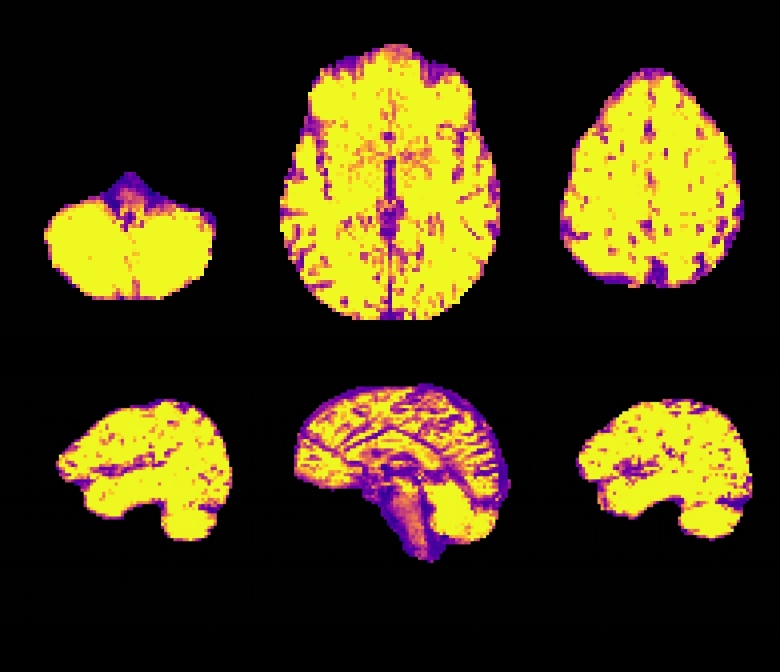
\includegraphics[width=3cm]{images/sub-001_ses-1_task-HABLA1200_OC_part-mag_bold_tmppca_tsnr_all.jpg} &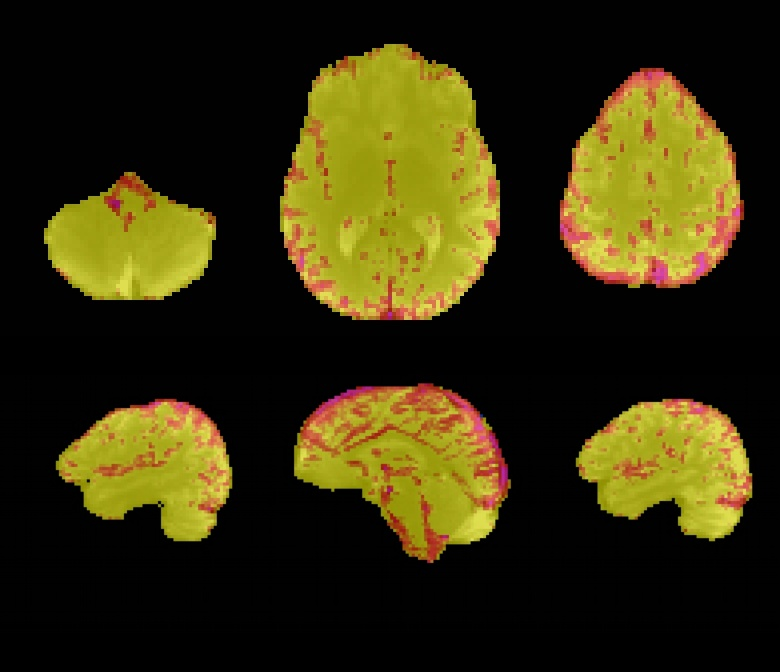
\includegraphics[width=3cm]{images/sub-001_ses-1_task-HABLA1200_OCspc_part-mag_bold_tmppca_all} &\textcolor{white}{$\Delta $} 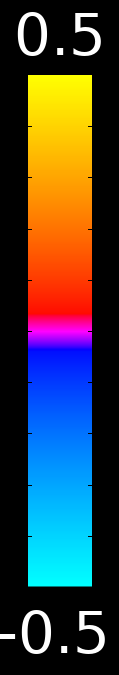
\includegraphics[width=.5cm]{images/SPC.png}\\
    \end{tabular}
    }
    \caption[tSNR  maps, Low resolution (2.4 mm isotropic)]{tSNR analysis at 2.4 mm (saturation limit 100 a.u.). Left: tSNR maps. Right: $\Delta$tSNR (change relative to vanilla).}
    \label{fig:tsnr1200}
\end{figure}
%-- scatterplot
\begin{figure}[htbp]
\raggedright
\captionsetup{justification=raggedleft, singlelinecheck=off}
\colorbox{white}{
    \raggedleft
    \begin{tabular}{>{\raggedright\arraybackslash}m{.7cm}>{\raggedright\arraybackslash}m{2.5cm}>{\raggedright\arraybackslash}m{2.5cm}>{\raggedright\arraybackslash}m{2.5cm}>{\raggedright\arraybackslash}m{2.5cm}}
       & \textcolor{black}{\textbf{MPPCA}}
       & \textcolor{black}{\textbf{NORDIC}}
       & \textcolor{black}{\textbf{HYDRA}}
       & \textcolor{black}{\textbf{TMPPCA}}\\
       \rotatebox[origin=l]{90}{\textcolor{black}{sub-001}}& 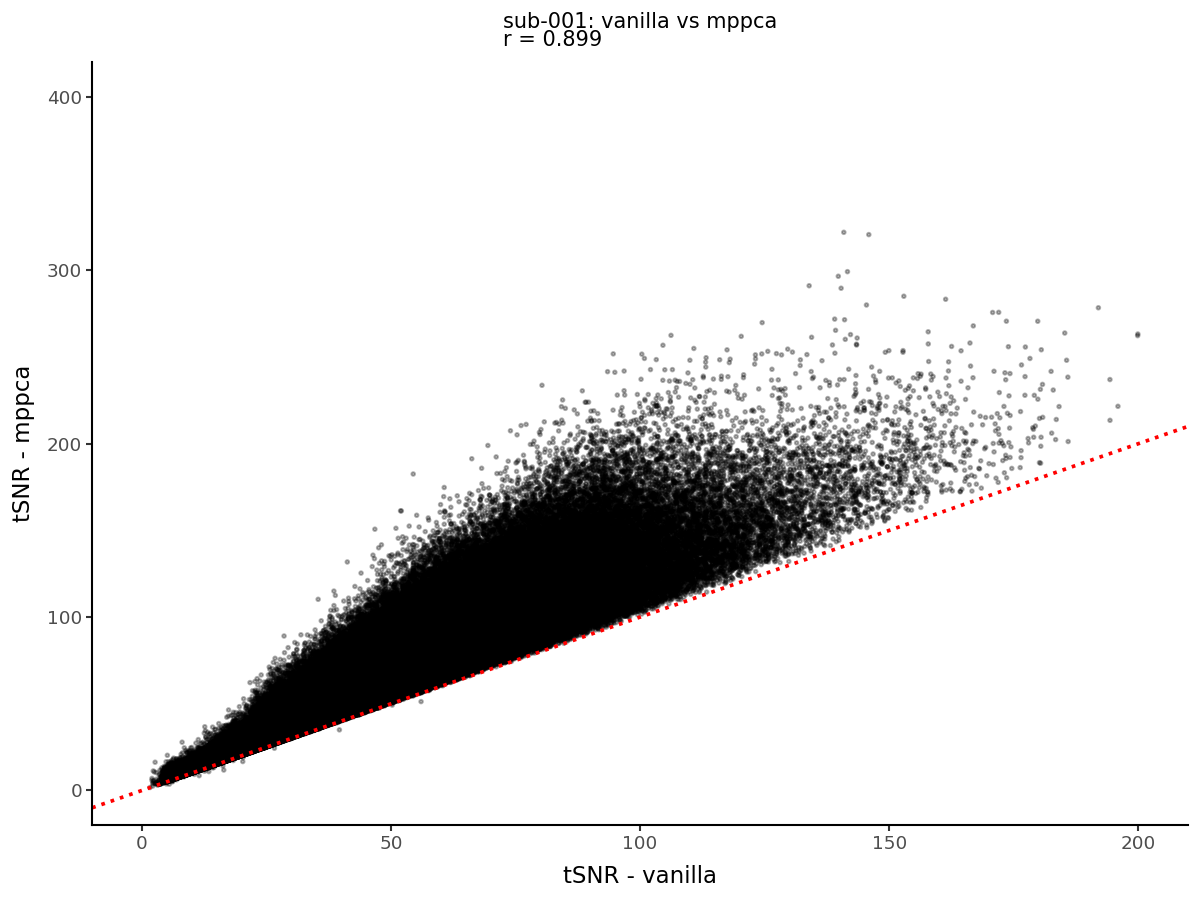
\includegraphics[width=2.5cm]{images/sub-001_vanilla_vs_mppca_tsnr_scatter1200.png}
       & 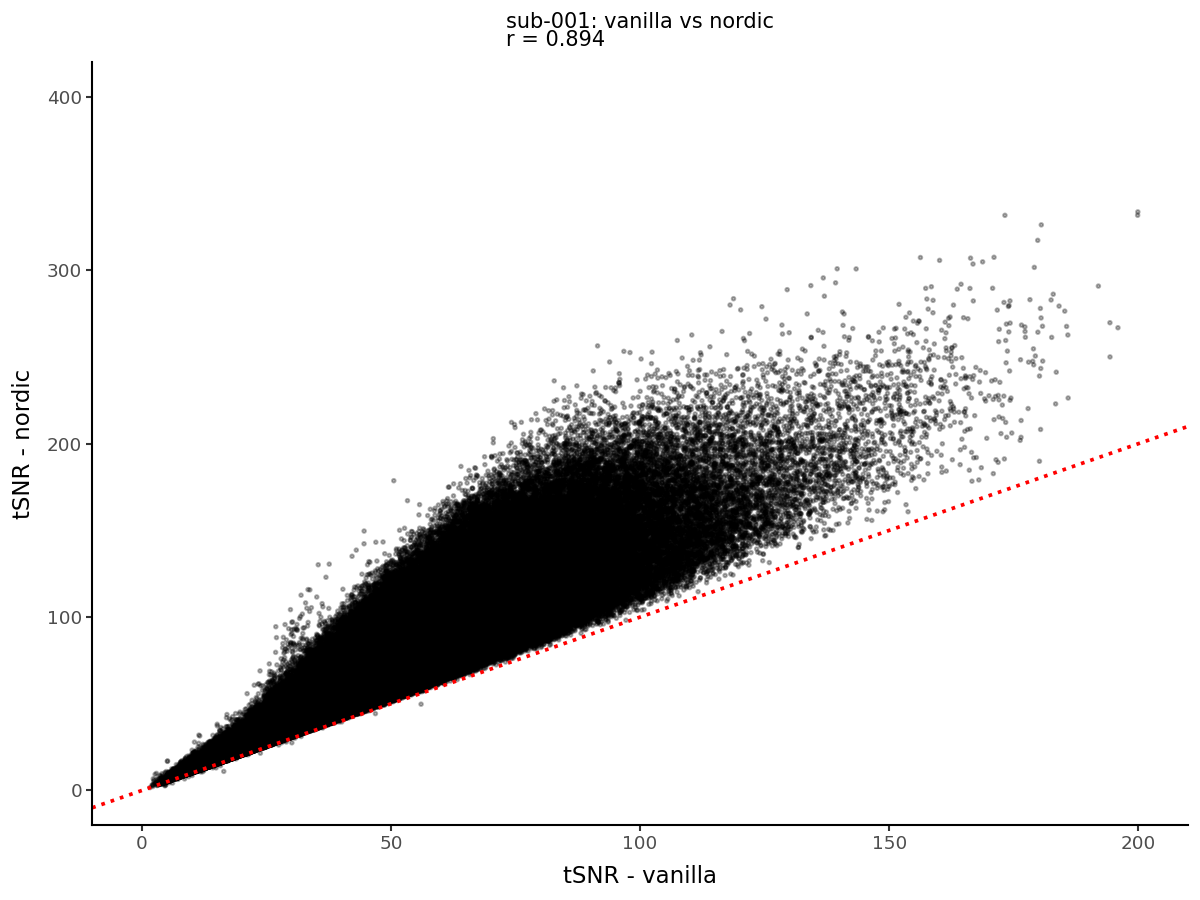
\includegraphics[width=2.5cm]{images/sub-001_vanilla_vs_nordic_tsnr_scatter1200.png}
       & 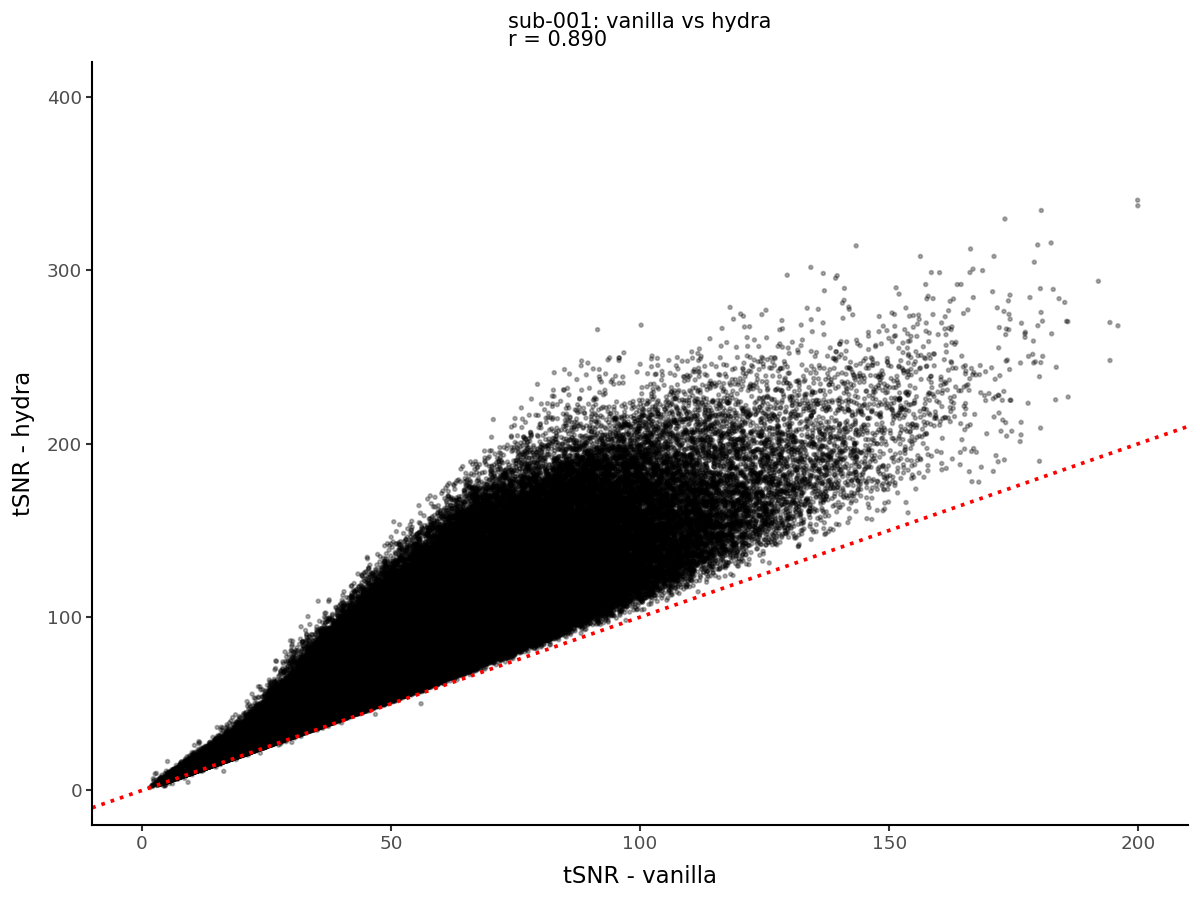
\includegraphics[width=2.5cm]{images/sub-001_vanilla_vs_hydra_tsnr_scatter1200.png}
       & 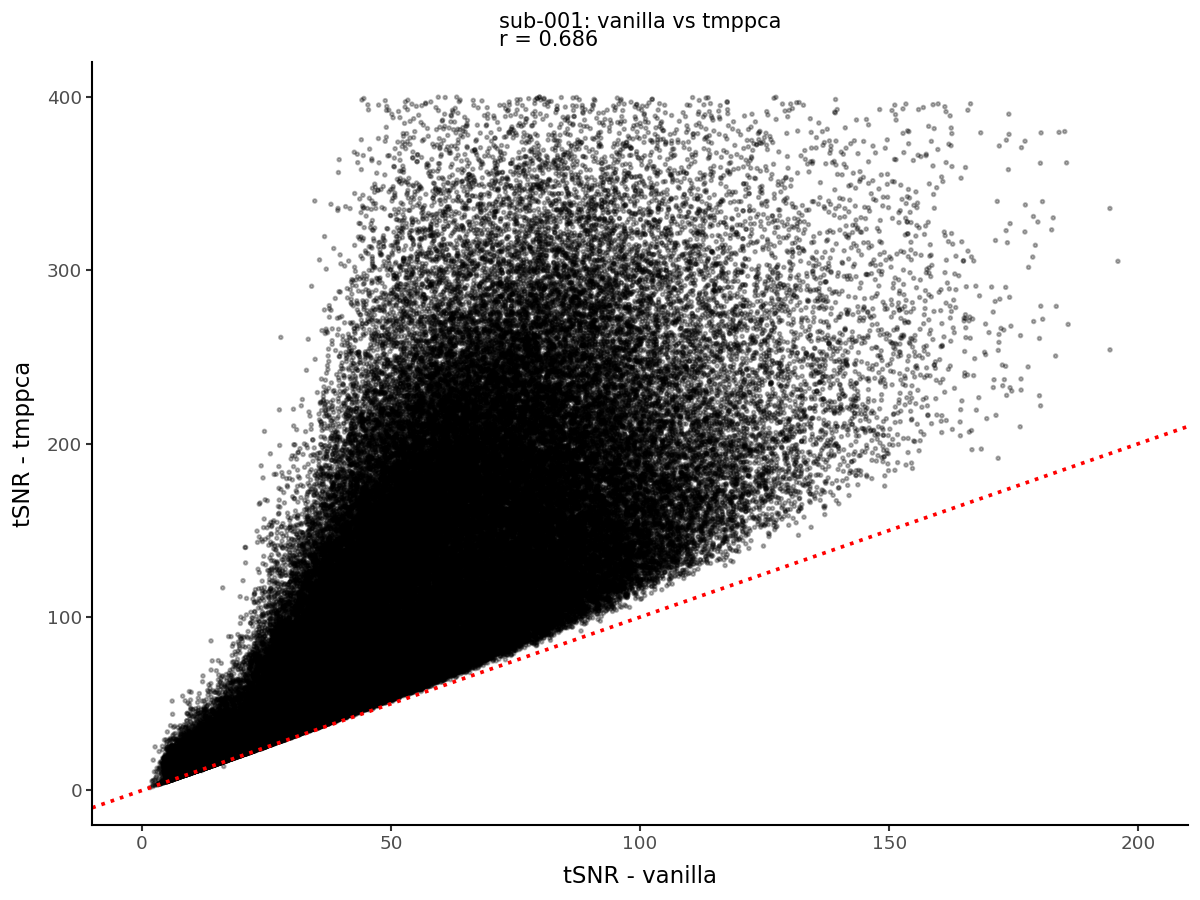
\includegraphics[width=2.5cm]{images/sub-001_vanilla_vs_tmppca_tsnr_scatter1200.png}\\
         \rotatebox[origin=l]{90}{\textcolor{black}{sub-002}}& 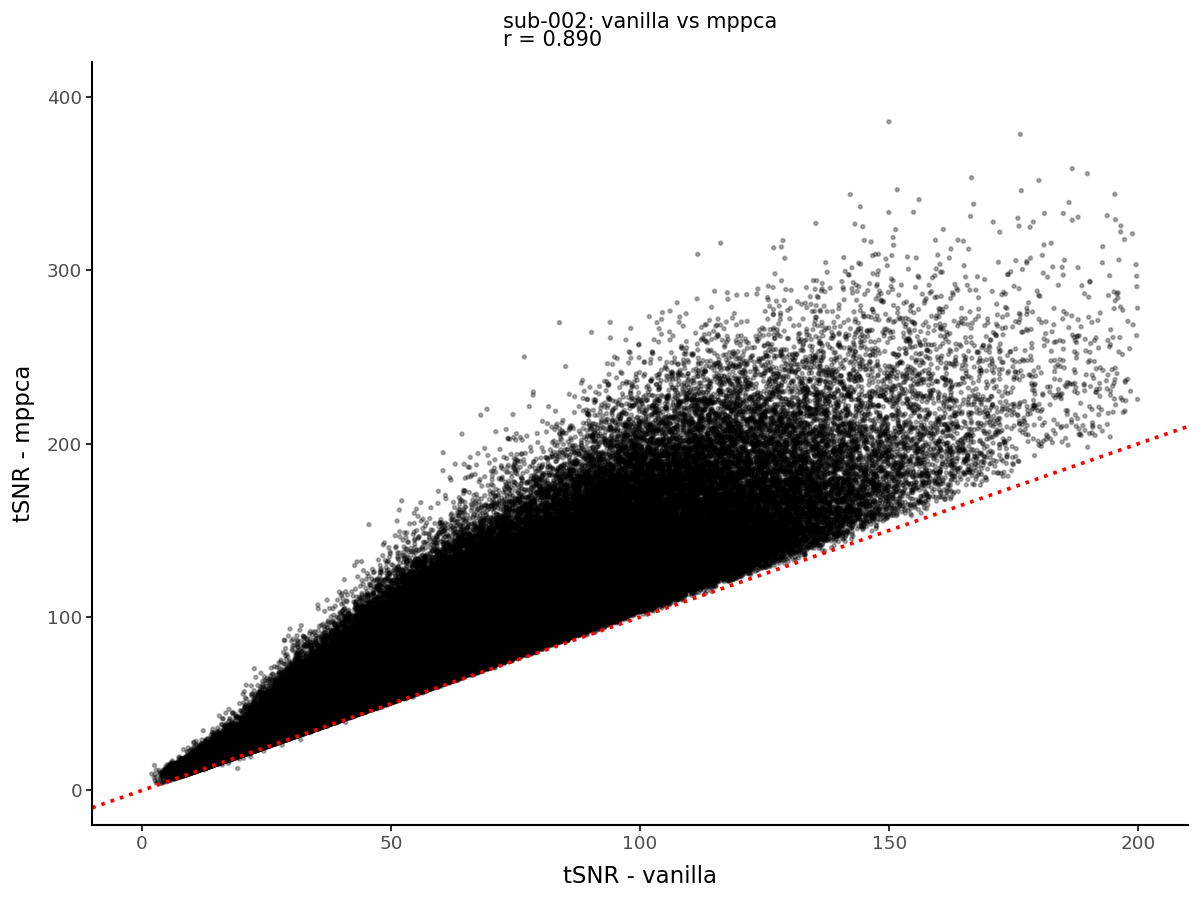
\includegraphics[width=2.5cm]{images/sub-002_vanilla_vs_mppca_tsnr_scatter1200.png}
       & 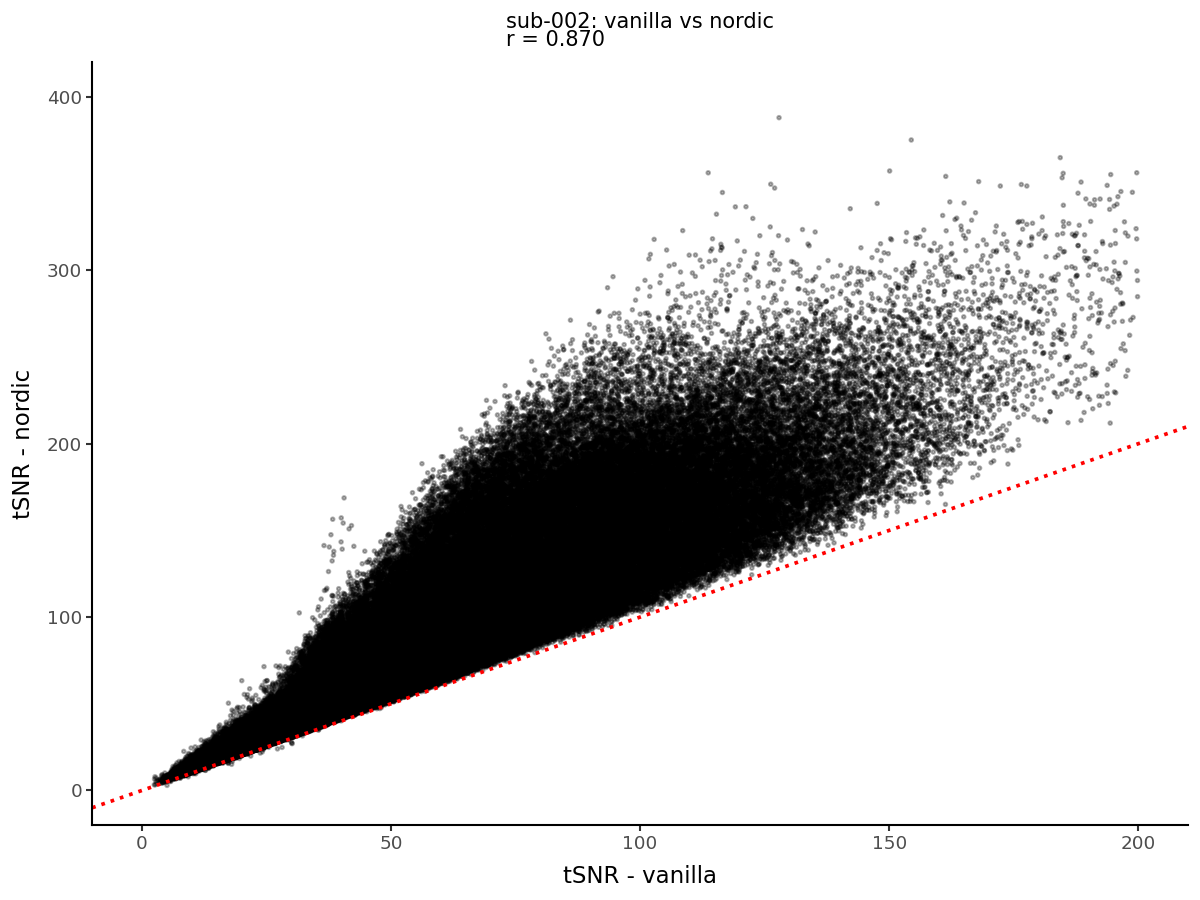
\includegraphics[width=2.5cm]{images/sub-002_vanilla_vs_nordic_tsnr_scatter1200.png}
       & 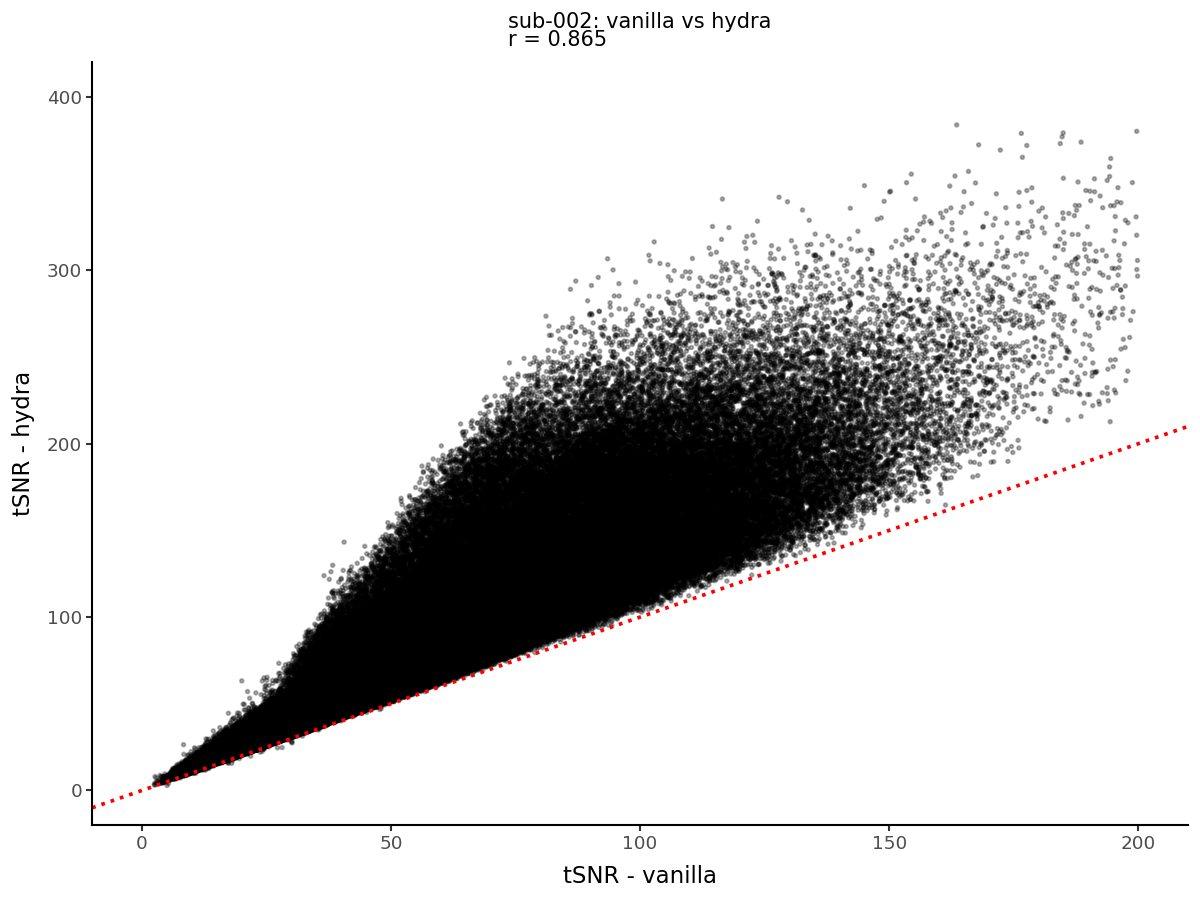
\includegraphics[width=2.5cm]{images/sub-002_vanilla_vs_hydra_tsnr_scatter1200.png}
       & 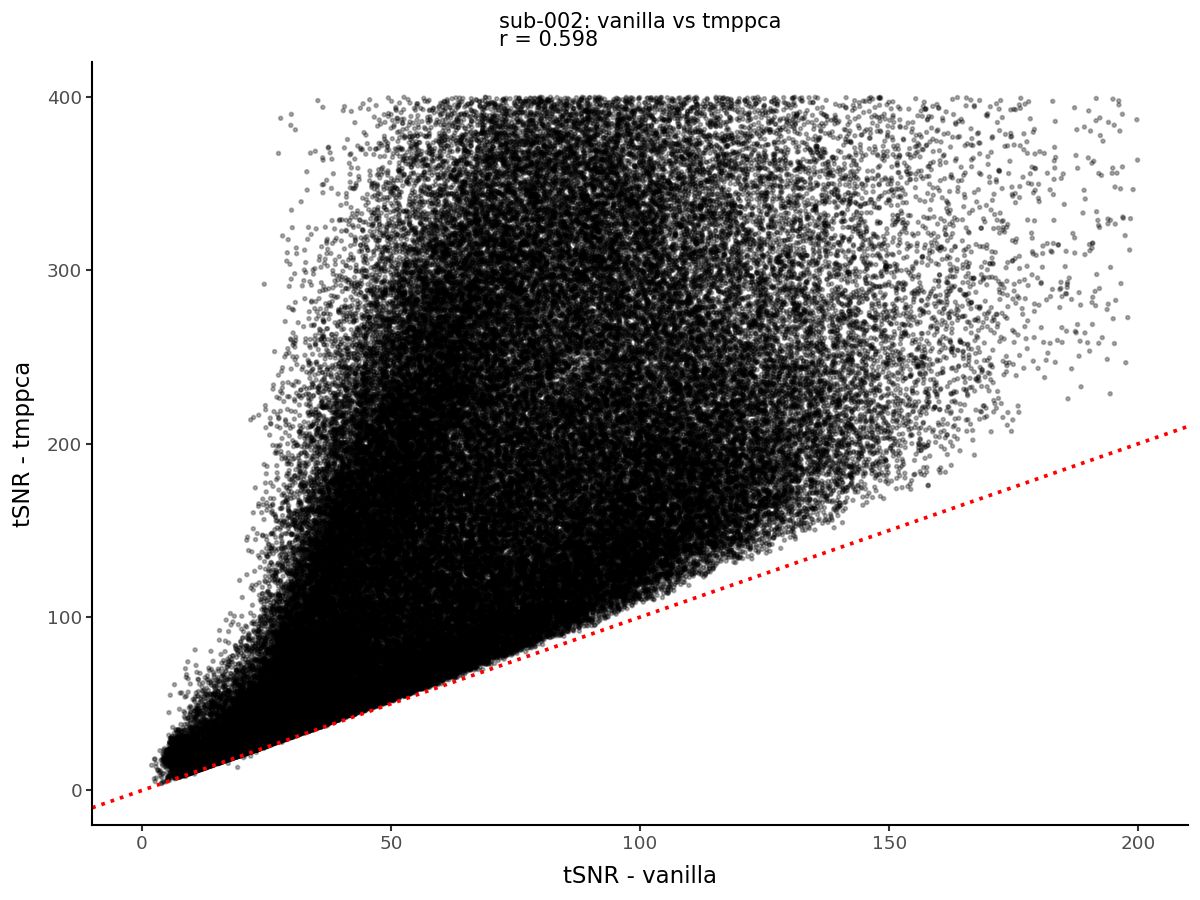
\includegraphics[width=2.5cm]{images/sub-002_vanilla_vs_tmppca_tsnr_scatter1200.png}\\
       \rotatebox[origin=l]{90}{\textcolor{black}{sub-003}}& 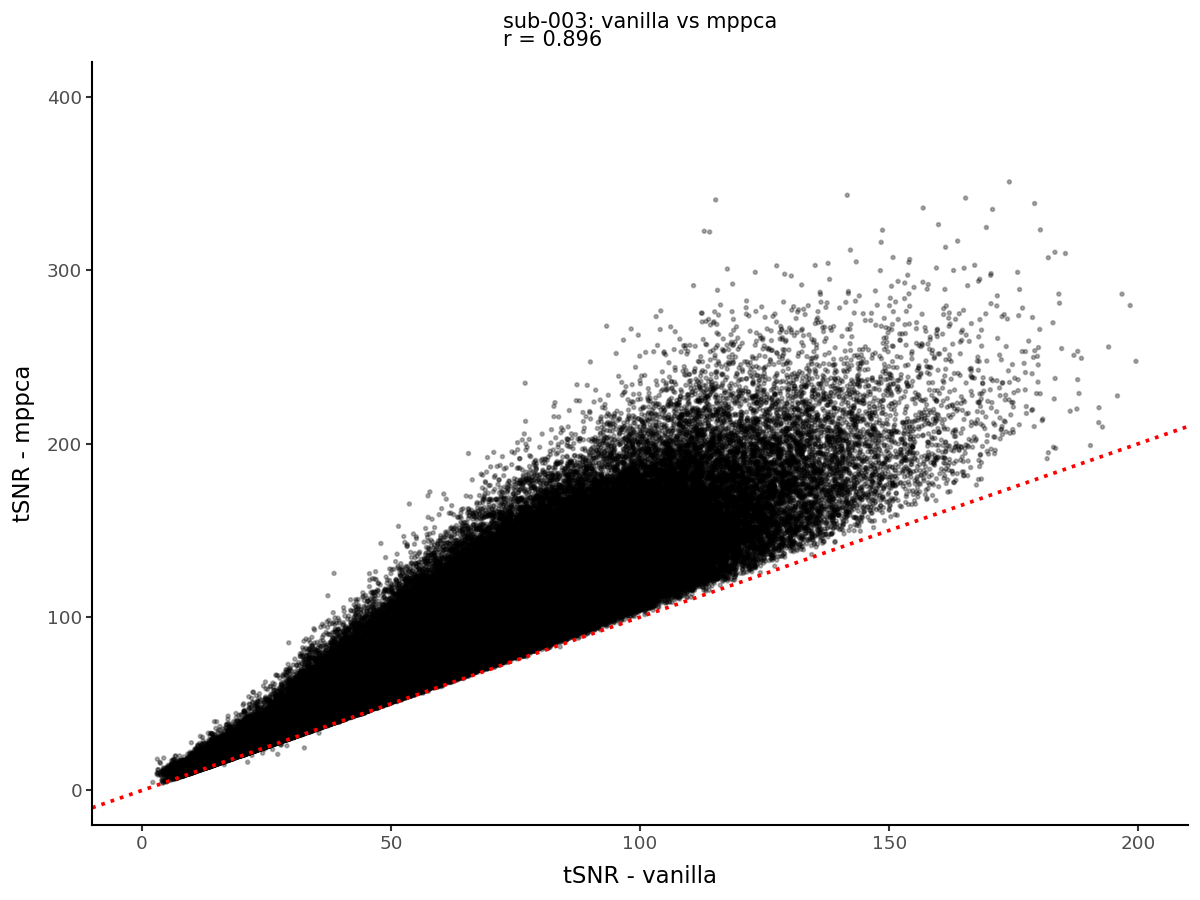
\includegraphics[width=2.5cm]{images/sub-003_vanilla_vs_mppca_tsnr_scatter1200.png}
       & 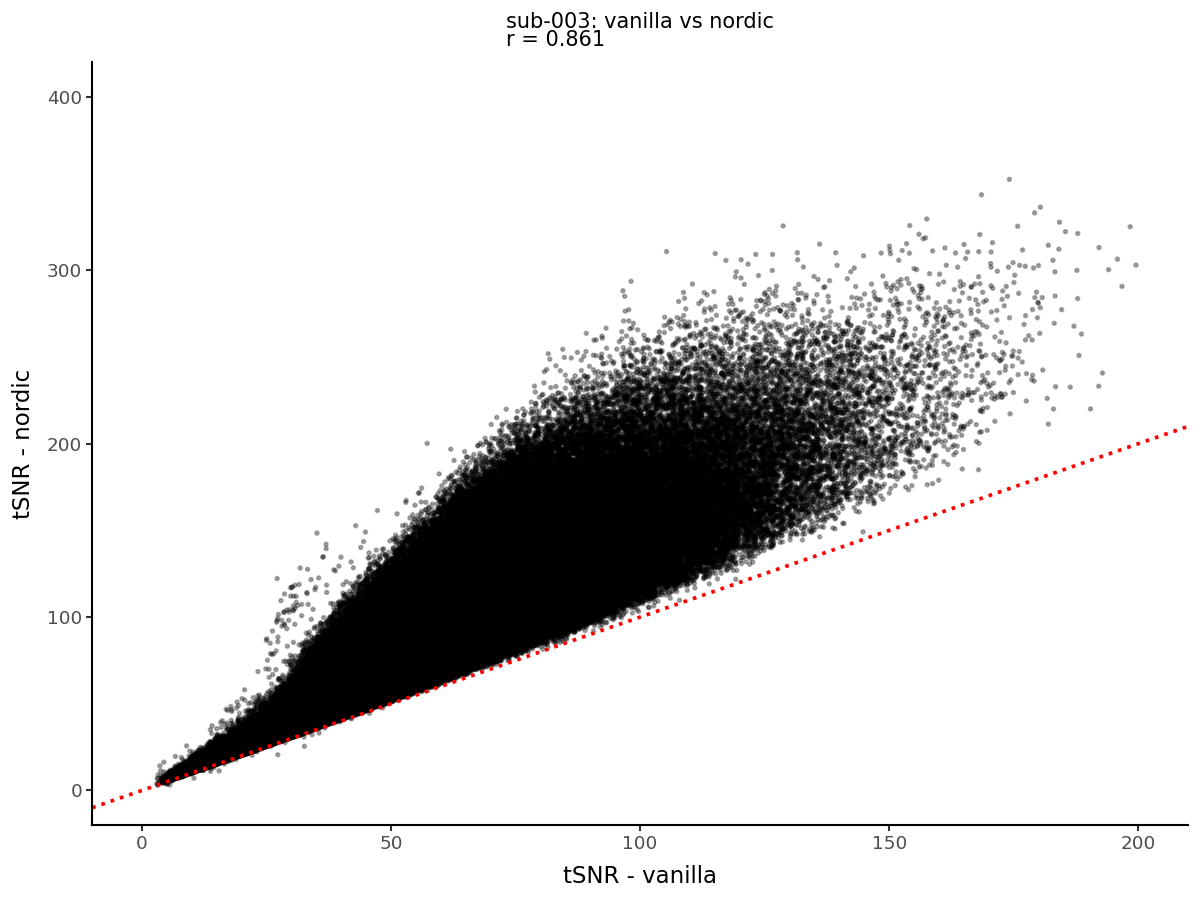
\includegraphics[width=2.5cm]{images/sub-003_vanilla_vs_nordic_tsnr_scatter1200.png}
       & 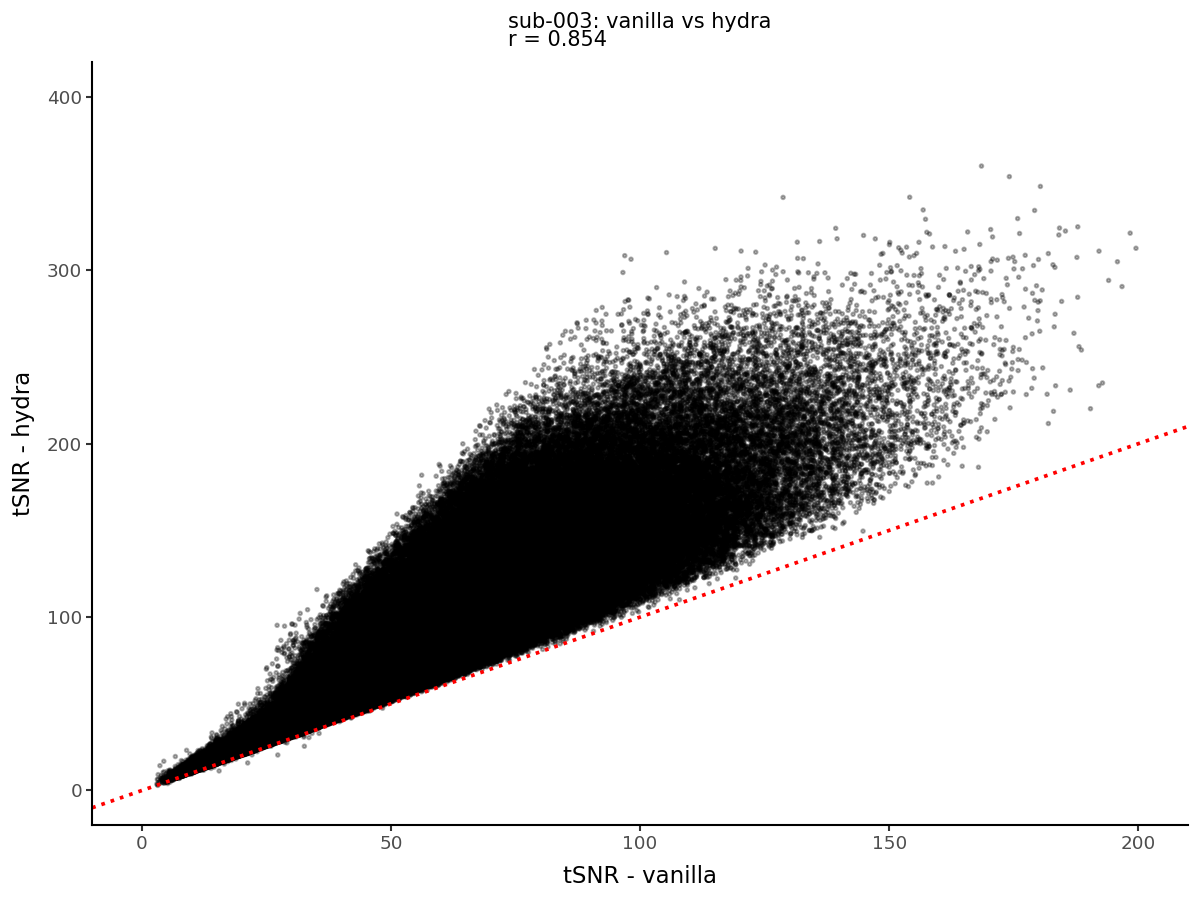
\includegraphics[width=2.5cm]{images/sub-003_vanilla_vs_hydra_tsnr_scatter1200.png}
       & 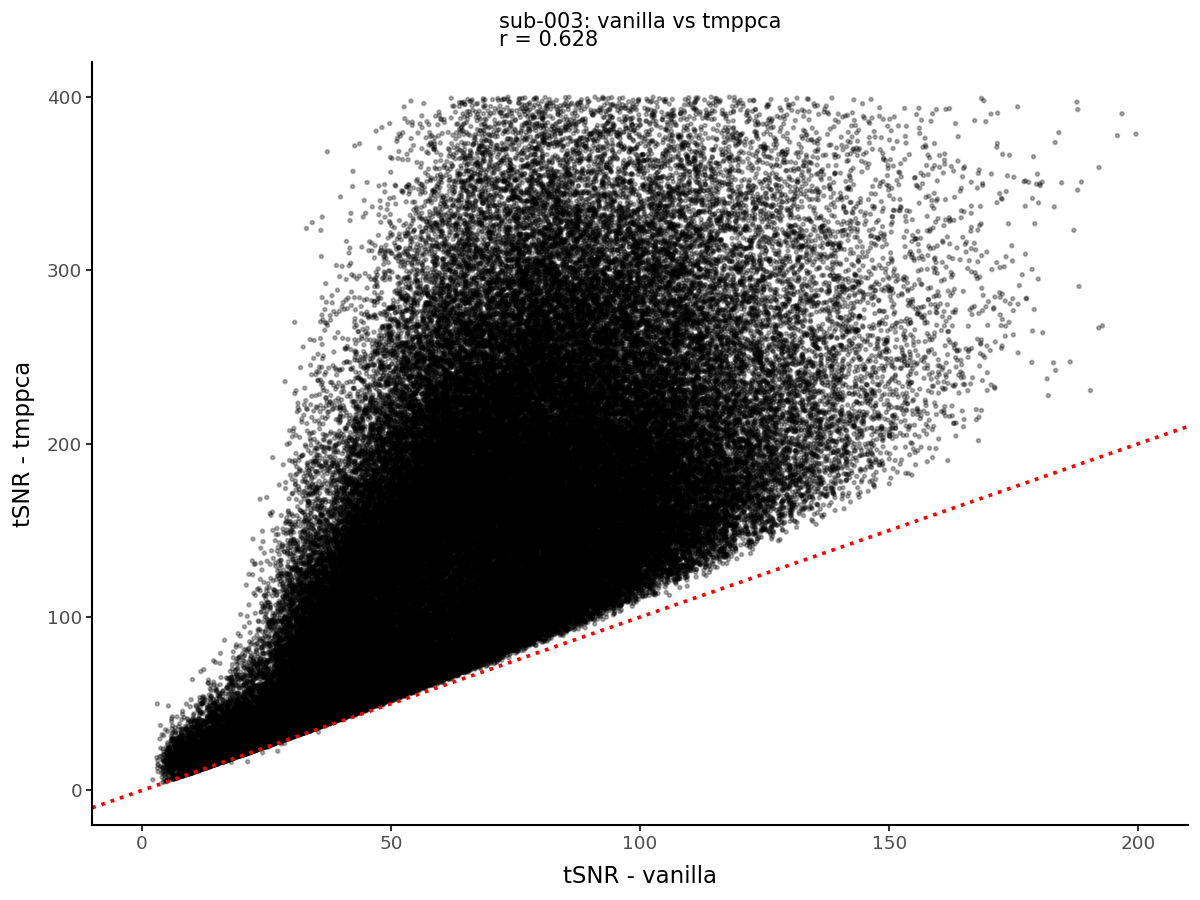
\includegraphics[width=2.5cm]{images/sub-003_vanilla_vs_tmppca_tsnr_scatter1200.png}\\
       \rotatebox[origin=l]{90}{\textcolor{black}{sub-004}}& 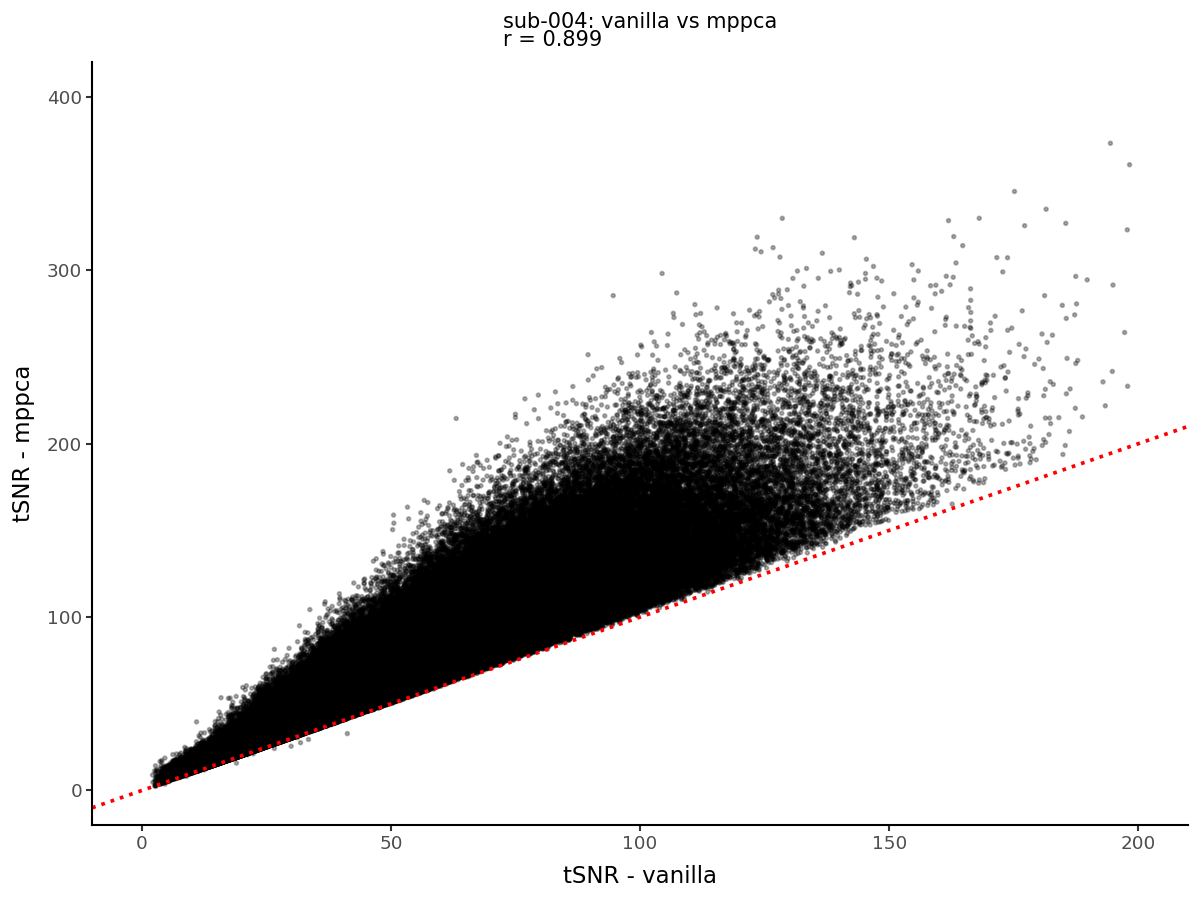
\includegraphics[width=2.5cm]{images/sub-004_vanilla_vs_mppca_tsnr_scatter1200.png}
       & 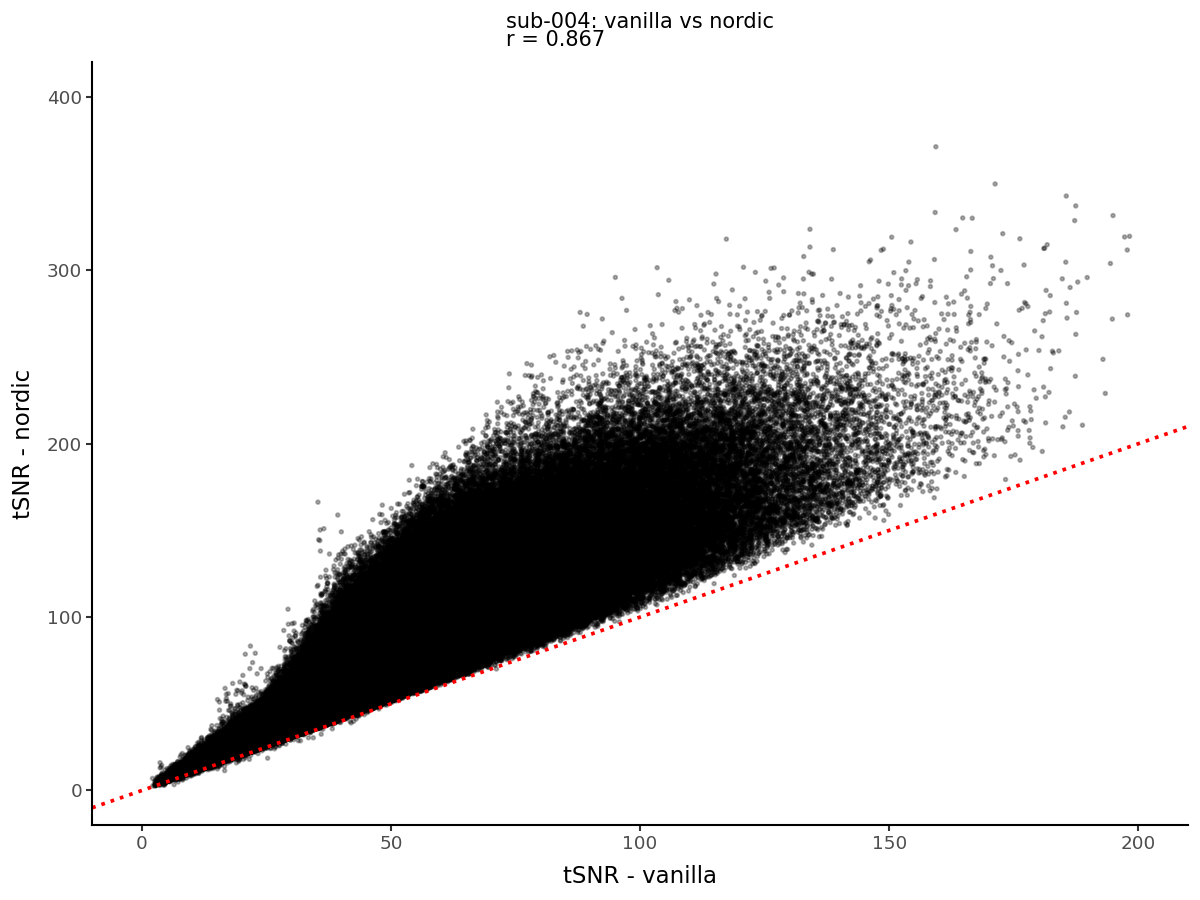
\includegraphics[width=2.5cm]{images/sub-004_vanilla_vs_nordic_tsnr_scatter1200.png}
       & 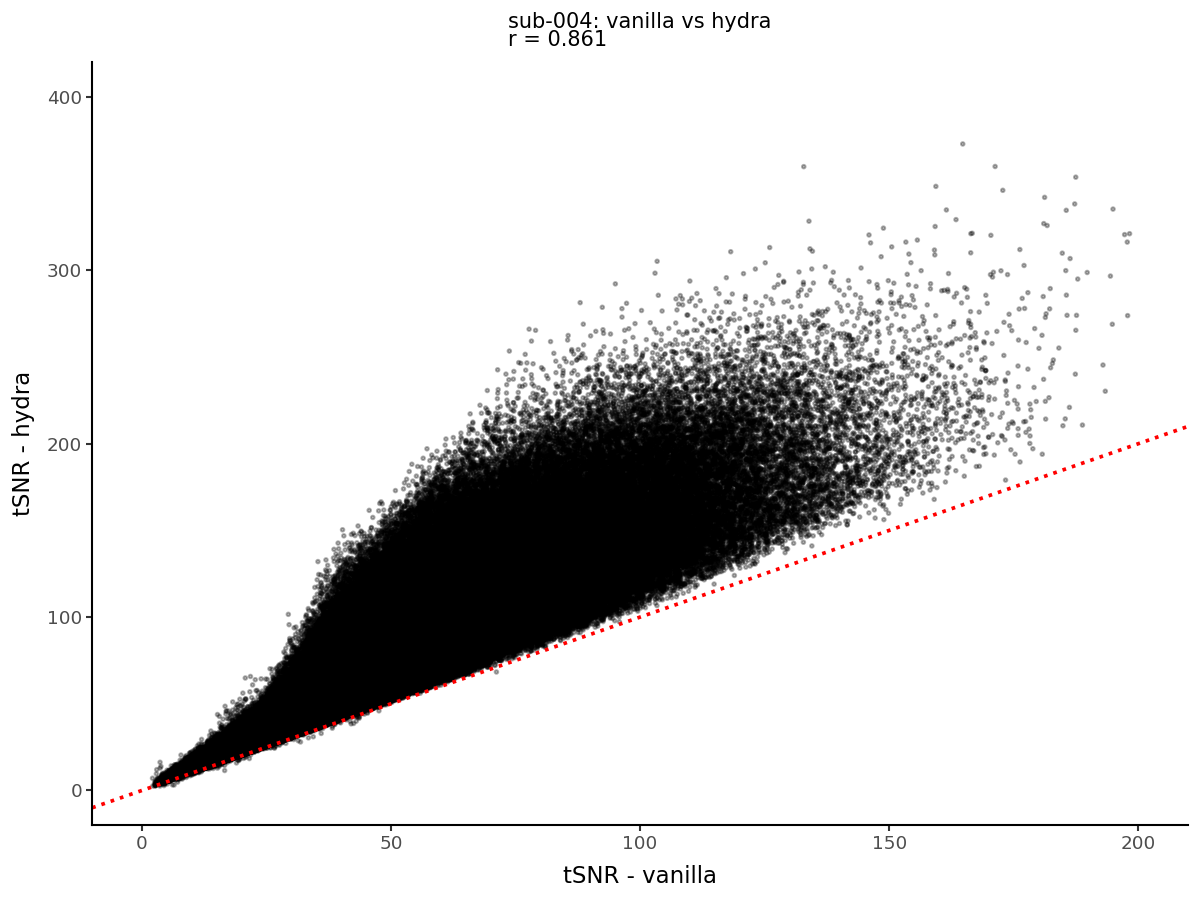
\includegraphics[width=2.5cm]{images/sub-004_vanilla_vs_hydra_tsnr_scatter1200.png}
       & 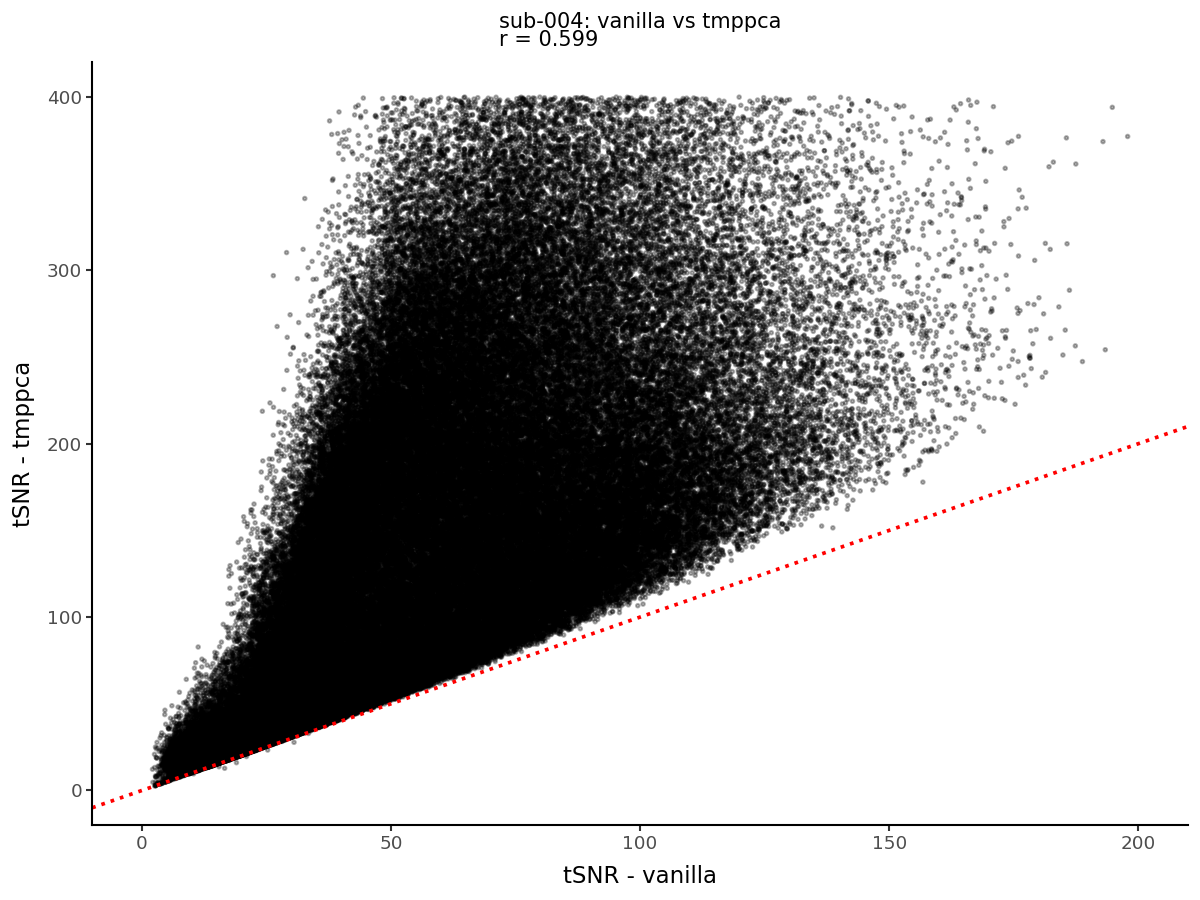
\includegraphics[width=2.5cm]{images/sub-004_vanilla_vs_tmppca_tsnr_scatter1200.png}\\
       \rotatebox[origin=l]{90}{\textcolor{black}{sub-005}}& 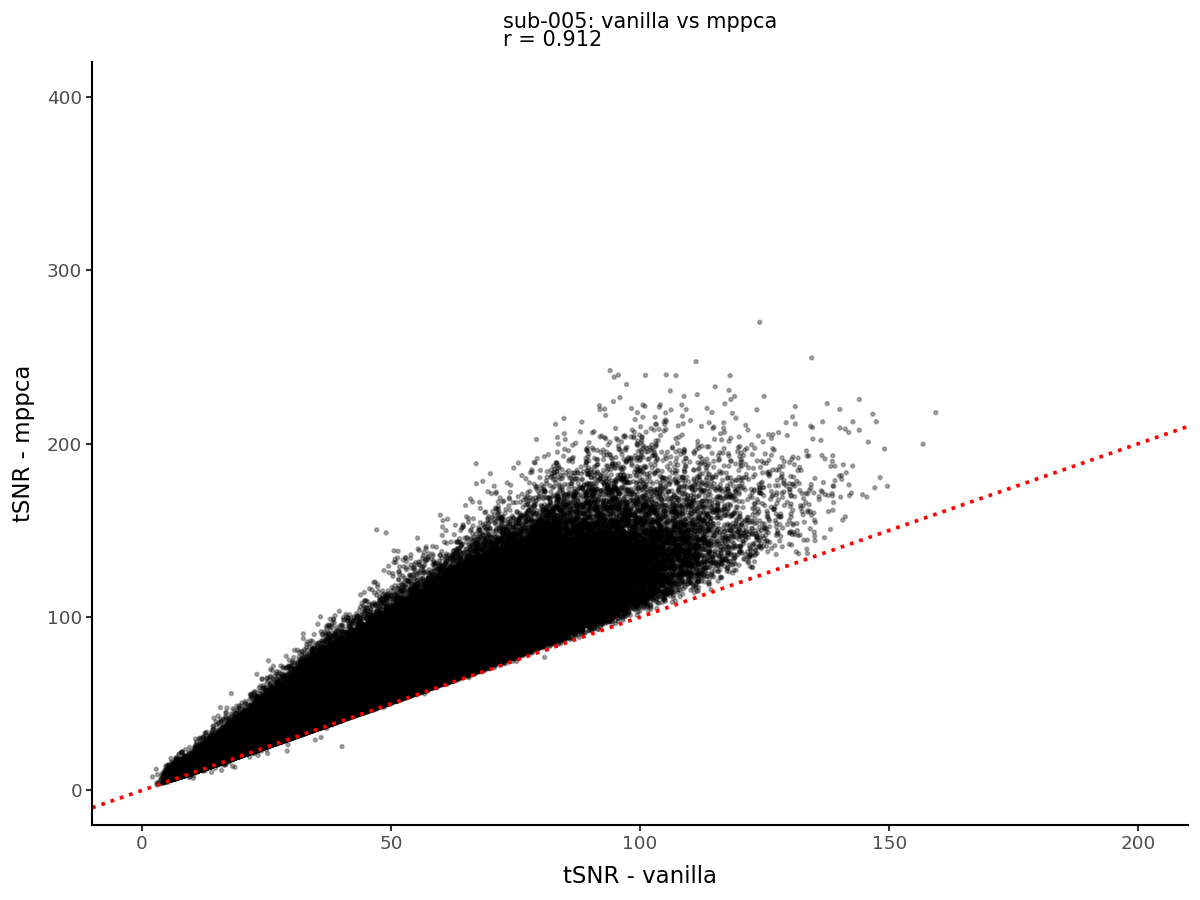
\includegraphics[width=2.5cm]{images/sub-005_vanilla_vs_mppca_tsnr_scatter1200.png}
       & 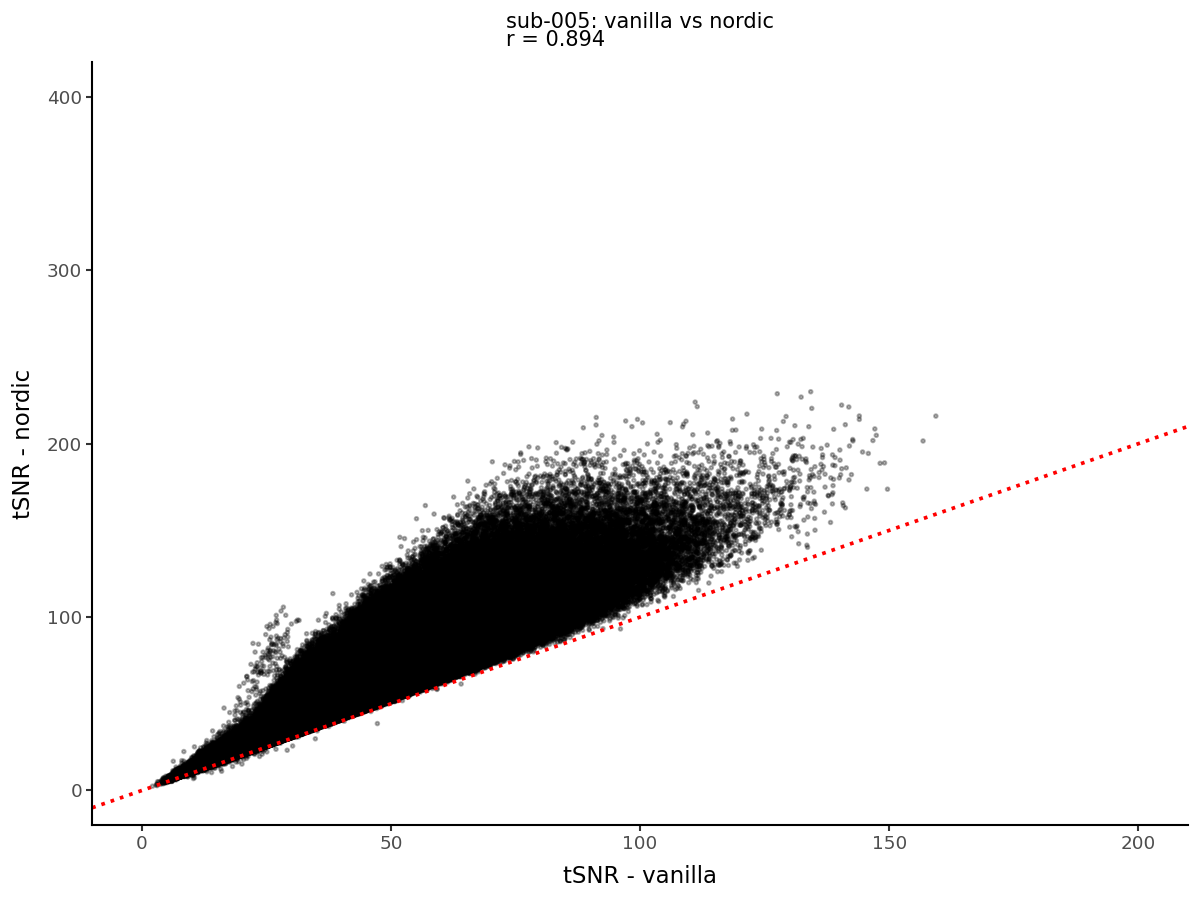
\includegraphics[width=2.5cm]{images/sub-005_vanilla_vs_nordic_tsnr_scatter1200.png}
       & 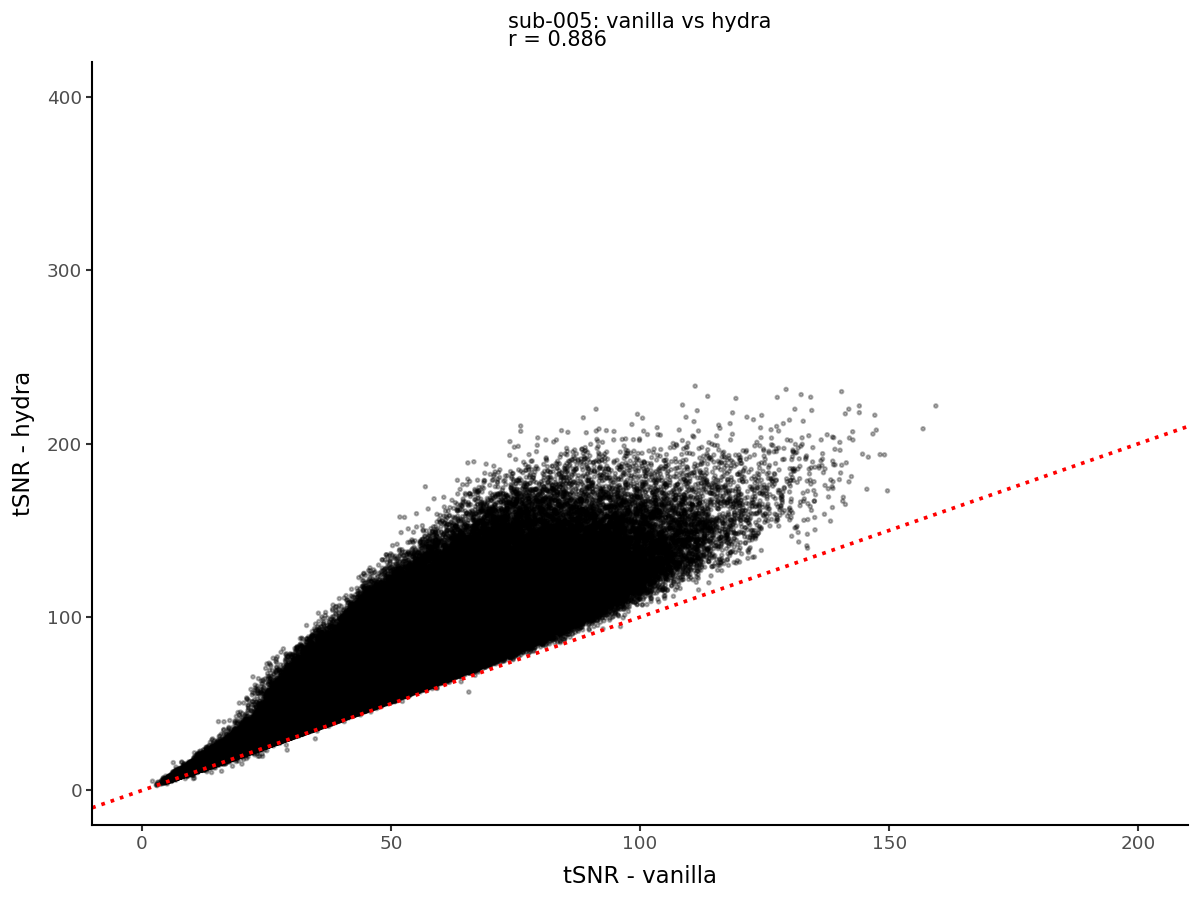
\includegraphics[width=2.5cm]{images/sub-005_vanilla_vs_hydra_tsnr_scatter1200.png}
       & 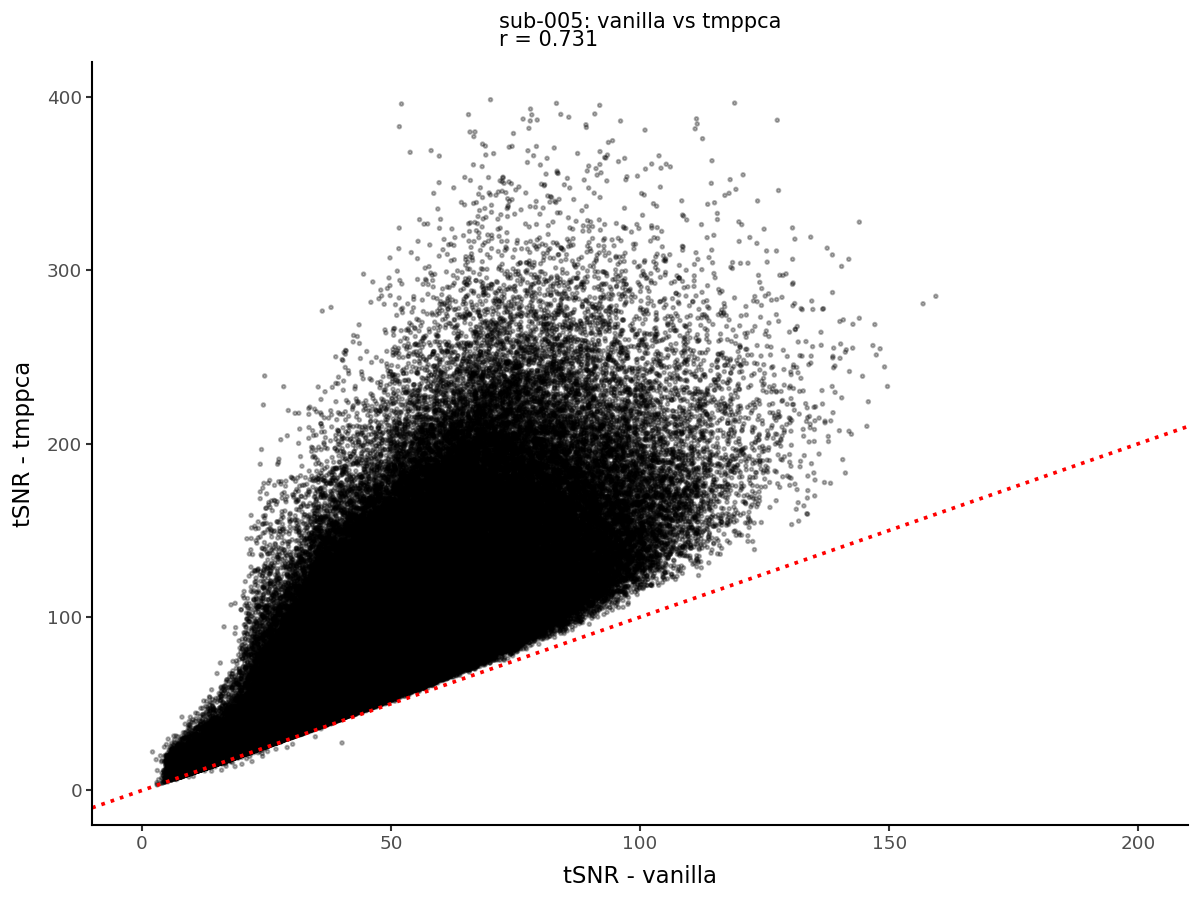
\includegraphics[width=2.5cm]{images/sub-005_vanilla_vs_tmppca_tsnr_scatter1200.png}\\
       \end{tabular}
    }
    \caption[tSNR scatterplots between methods, 2.4 mm]{tSNR scatterplots (2.4 mm, per subject) of vanilla tSNR (x) vs. denoised tSNR (y). Identity line (red) = no change.}
    \label{fig:scatter1200}
\end{figure}

For the 2.4 mm resolution dataset, the left panel of Fig.~\ref{fig:tsnr1200} illustrates that tSNR demonstrated a pronounced widespread increase following the application of thermal denoising. Consistent with findings from single-echo acquisitions, NORDIC yields higher tSNR values than MPPCA, whereas TMPPCA provides the highest tSNR among all evaluated denoising approaches. The greatest improvement was observed with TMPPCA, followed by NORDIC and then HYDRA. Notably, brain regions characterized by intrinsically low SNR due to their distance from the head coils, such as deep brain and subcortical structures, exhibit marked gains in signal quality.  The right panel shows $\Delta$tSNR maps, representing the change in tSNR relative to the vanilla (non-denoised) data used as baseline. These maps further confirm that TMPPCA outperforms all other methods, as indicated by the larger extent of saturation. These maps exhibited predominantly positive saturation, with changes frequently exceeding a 50\% increase (i.e. $\Delta \text{tSNR} > 0.5$).

To further quantify this effect, we examined the relationship between per-voxel tSNR values the different denoising approaches using scatterplots versus baseline (“vanilla”) tSNR values (Fig.~\ref{fig:scatter1200}). In the absence of any denoising effect, the data points are expected to align closely with the identity line (red line), indicating a linear relationship with unit slope and no systematic deviation. Deviations of the point cloud from this identity line (either above or below) quantify the voxelwise magnitude and direction of tSNR change. For all subjects, the scatterplots show a global increase in tSNR with all denoising methods, with TMPPCA yielding the greatest positive shift, reflecting the highest per‑voxel gains.

A similar pattern of increase in tSNR after thermal denoising was observed for the 2 mm dataset (Fig.~\ref{fig:tsnr1700}). As with the 2.4 mm data, TMPPCA yielded the most noticeable improvement, followed by NORDIC and HYDRA. The $\Delta\%tSNR$ maps were again predominantly positively saturated, with changes larger than 0.5. This consistency across the two low resolution datasets is likely attributable to both operating within a tSNR regime, where physiological fluctuations, rather than thermal noise, are the dominant source of signal variance due to the multi-channel coil array configuration, and the use of parallel imaging (GRAPPA acceleration $R$=2) and partial Fourier \citep{triantafyllouPhysiologicalNoiseSignaltonoise2011}, along with the averaging effect of the multi-echo combination.

The scatterplot of per-voxel tSNR values further corroborated these findings, with TMPPCA demonstrating the greatest effect on increasing tSNR across all subjects (Fig.~\ref{fig:scatter1700}). Notably, the voxel distribution in the vanilla-TMPPCA scatterplots was more tightly clustered around compared to that of the 2.4 mm dataset. This more constrained distribution provides evidence that the 2 mm dataset resides in a slightly lower tSNR regime.

Consistent with qualitative impressions with low resolution datasets from the tSNR maps, all evaluated denoising methods increase tSNR (TMPPCA $>$ NORDIC $\simeq$ HYDRA $>$ MPPCA $>$ VANILLA). In particular, TMPPCA exhibits a pronounced positive shift, with the scatter markedly skewed towards higher tSNR values, indicating a substantial per-voxel improvement in tSNR.


%%%%%  -- 2   mm -- %%%%%
\begin{figure}[htbp]
\centering \colorbox{black}{
    \centering
    \begin{tabular}{>{\centering\arraybackslash}m{.5cm}>{\centering\arraybackslash}m{3cm}>{\centering\arraybackslash}m{3cm}>{\centering\arraybackslash}m{.5cm}}
    
       & \textcolor{white}{\textbf{tSNR}} & \textcolor{white}{\textbf{$\Delta tSNR$}}& \\
   \rotatebox[origin=l]{90}{\textcolor{white}{VANILLA}}
  &    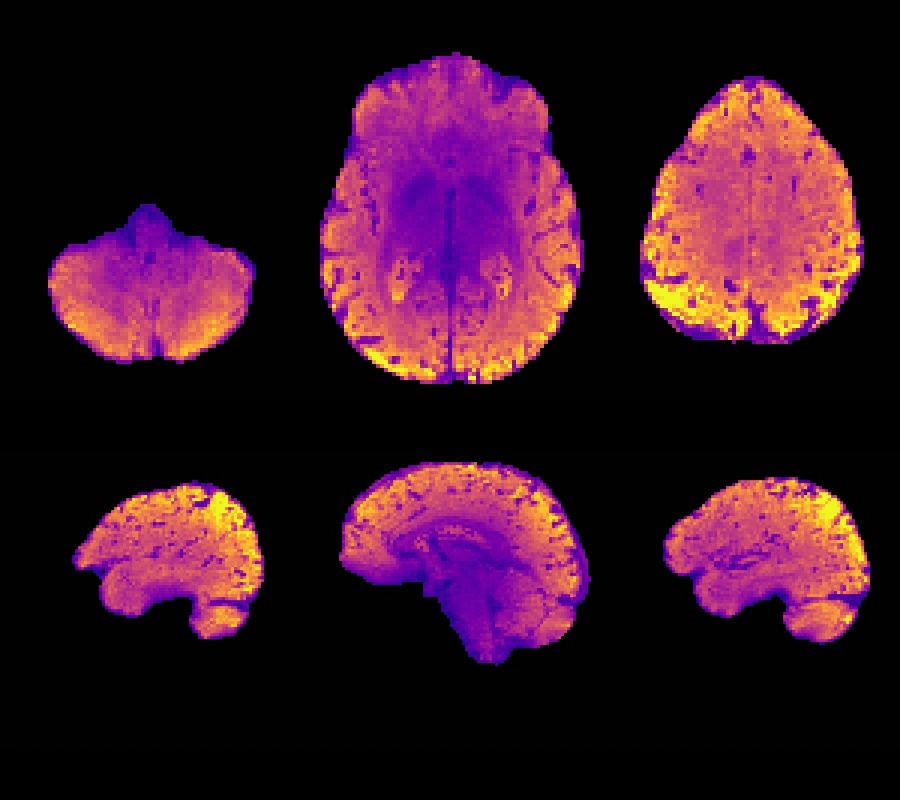
\includegraphics[width=3cm]{images/sub-001_ses-1_task-HABLA1700_OC_part-mag_bold_vanilla_tsnr_all.jpg} & & \textcolor{white}{tSNR} 
\includegraphics[width=.5cm]{images/Plasmatsnr.png}\\
     \rotatebox[origin=l]{90}{\textcolor{white}{MPPCA}}
  &    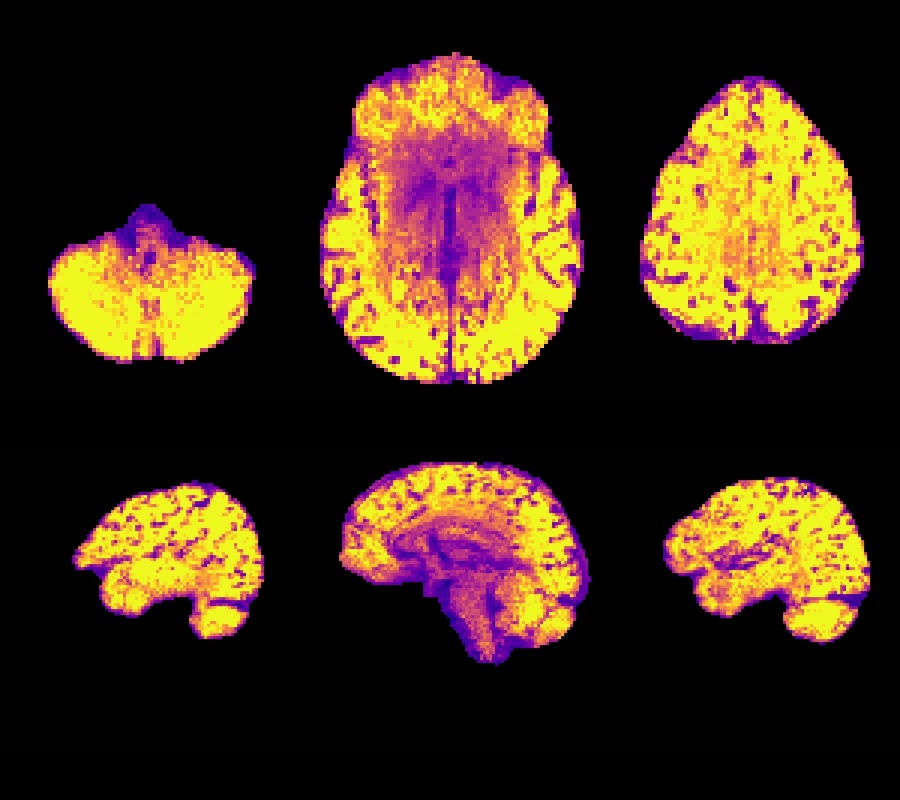
\includegraphics[width=3cm]{images/sub-001_ses-1_task-HABLA1700_OC_part-mag_bold_mppca_tsnr_all} &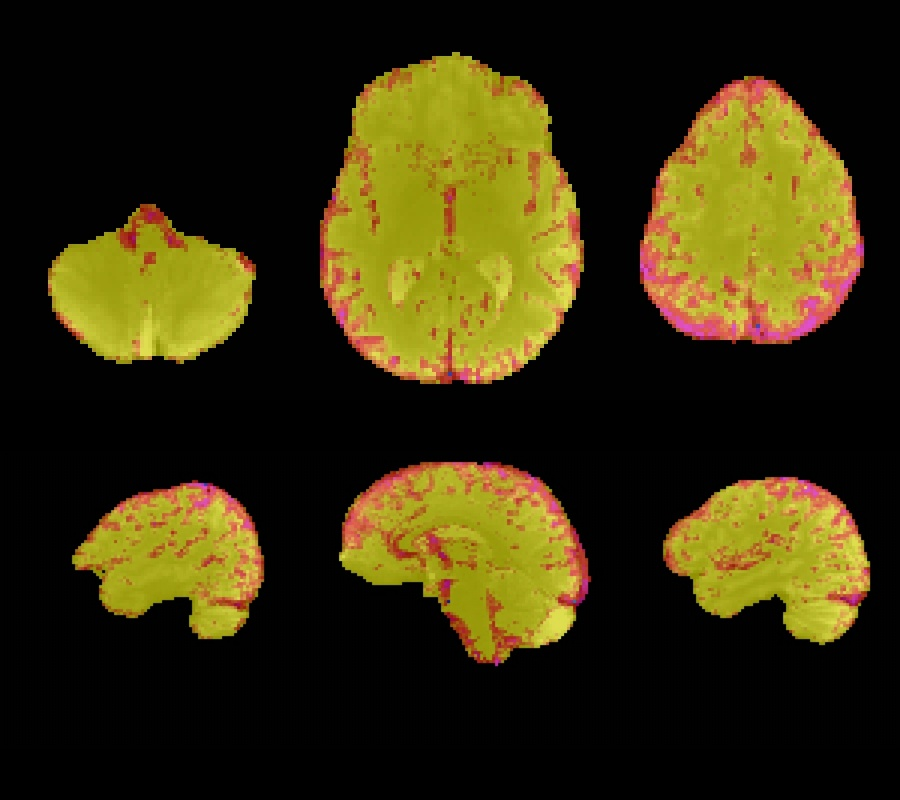
\includegraphics[width=3cm]{images/sub-001_ses-1_task-HABLA1700_OCspc_part-mag_bold_mppca_all} &\\
       \rotatebox[origin=l]{90}{\textcolor{white}{NORDIC}}
  &    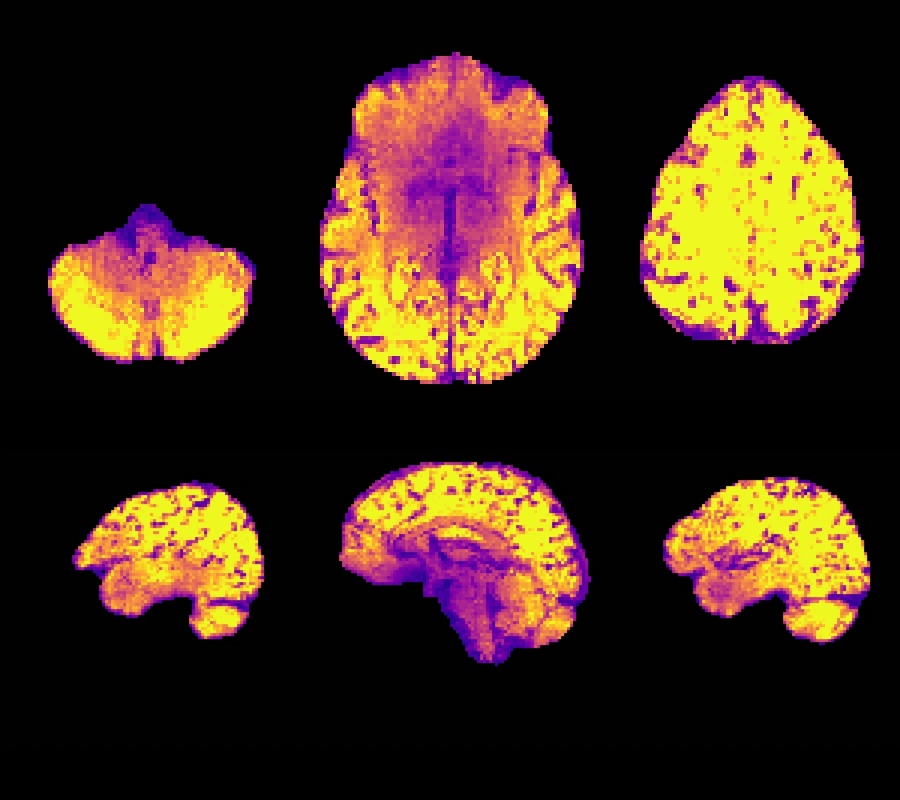
\includegraphics[width=3cm]{images/sub-001_ses-1_task-HABLA1700_OC_part-mag_bold_nordic_tsnr_all.jpg} &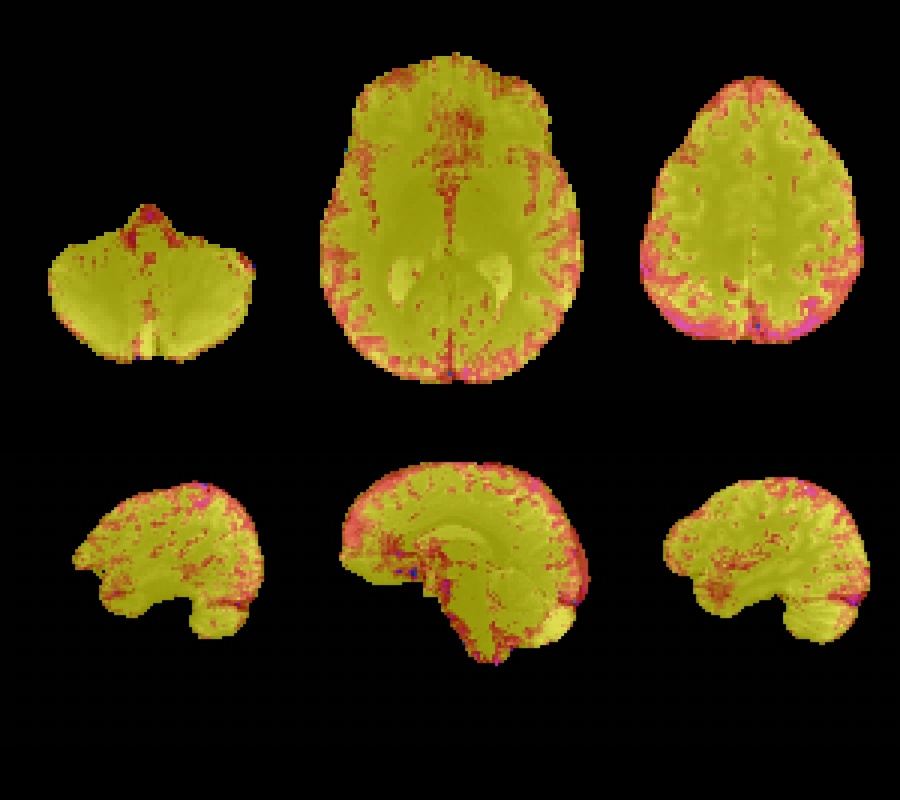
\includegraphics[width=3cm]{images/sub-001_ses-1_task-HABLA1700_OCspc_part-mag_bold_nordic_all} &\\
       \rotatebox[origin=l]{90}{\textcolor{white}{HYDRA}}
  &    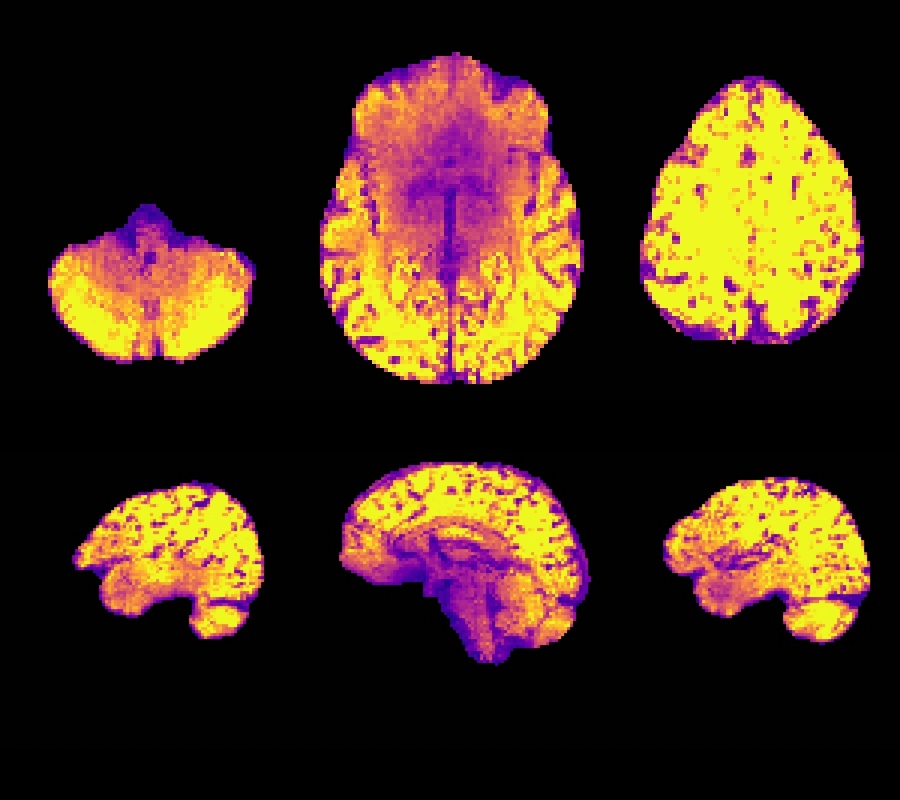
\includegraphics[width=3cm]{images/sub-001_ses-1_task-HABLA1700_OC_part-mag_bold_hydra_tsnr_all.jpg} &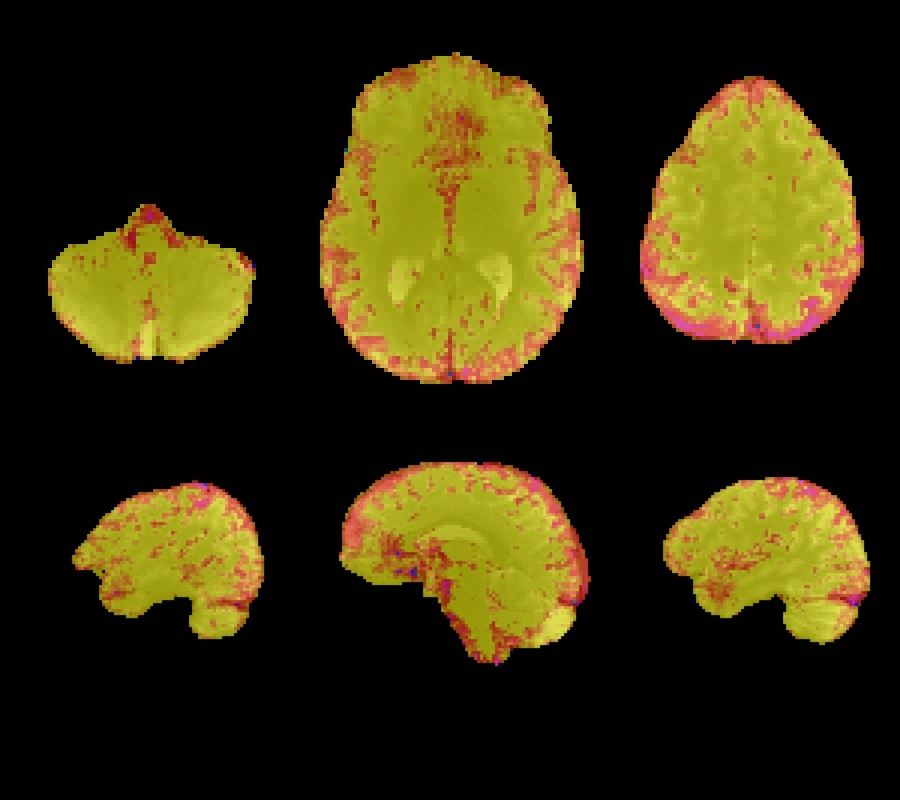
\includegraphics[width=3cm]{images/sub-001_ses-1_task-HABLA1700_OCspc_part-mag_bold_hydra_all} &\\
       \rotatebox[origin=l]{90}{\textcolor{white}{TMPPCA}}
  &    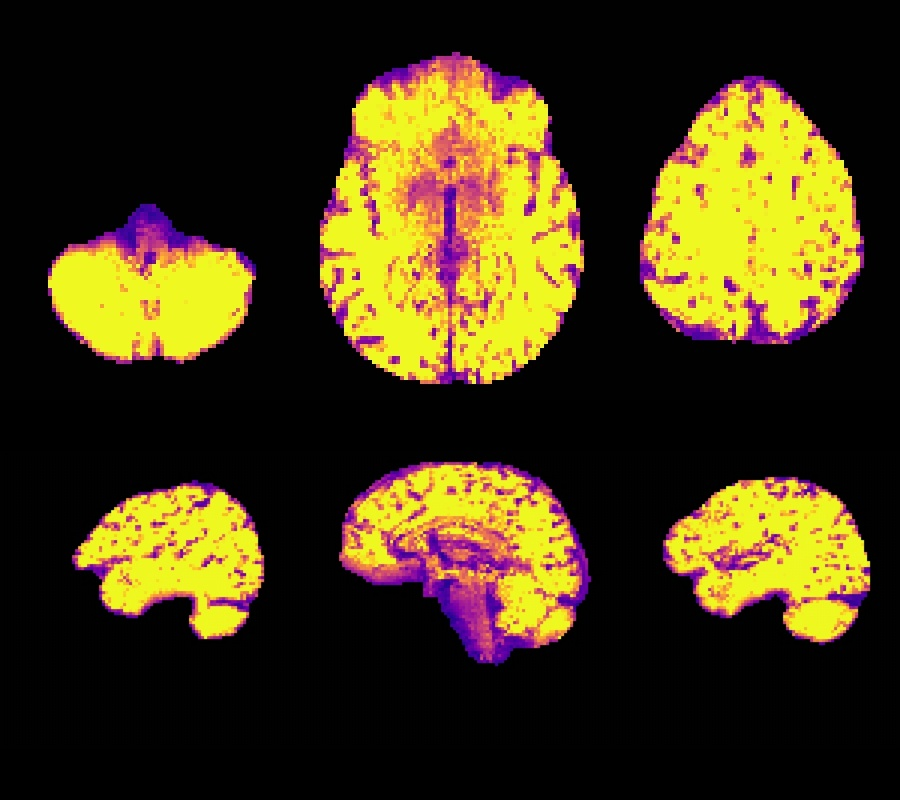
\includegraphics[width=3cm]{images/sub-001_ses-1_task-HABLA1700_OC_part-mag_bold_tmppca_tsnr_all.jpg} &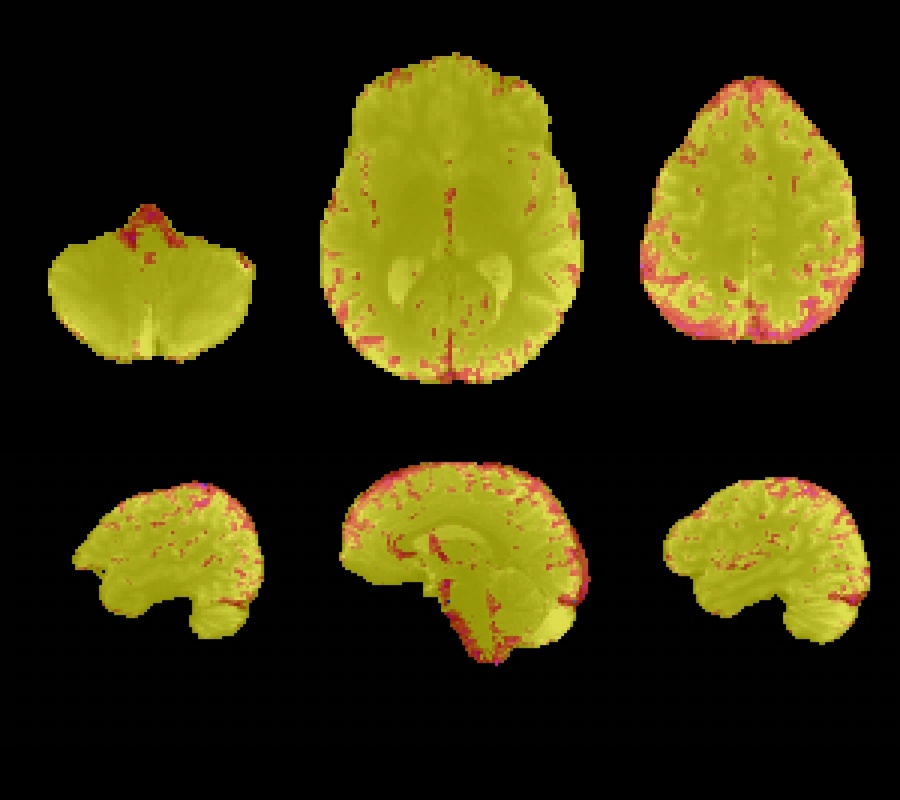
\includegraphics[width=3cm]{images/sub-001_ses-1_task-HABLA1700_OCspc_part-mag_bold_tmppca_all} &\textcolor{white}{$\Delta $} 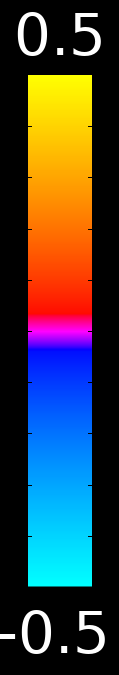
\includegraphics[width=.5cm]{images/SPC.png}\\
    \end{tabular}
    }
    \caption[tSNR  maps, Low resolution (2 mm isotropic)]{tSNR analysis at 2 mm (saturation limit 100 a.u.). Left: tSNR maps. Right: $\Delta$tSNR maps (change relative to vanilla).}
    \label{fig:tsnr1700}
\end{figure}
%-- scatterplot
\begin{figure}[htbp]
\raggedright
\captionsetup{justification=raggedleft, singlelinecheck=off} \colorbox{white}{
    \raggedleft
    \begin{tabular}{>{\raggedright\arraybackslash}m{.7cm}>{\raggedright\arraybackslash}m{2.5cm}>{\raggedright\arraybackslash}m{2.5cm}>{\raggedright\arraybackslash}m{2.5cm}>{\raggedright\arraybackslash}m{2.5cm}}
       & \textcolor{black}{\textbf{MPPCA}}
       & \textcolor{black}{\textbf{NORDIC}}
       & \textcolor{black}{\textbf{HYDRA}}
       & \textcolor{black}{\textbf{TMPPCA}}\\
       \rotatebox[origin=l]{90}{\textcolor{black}{sub-001}}& 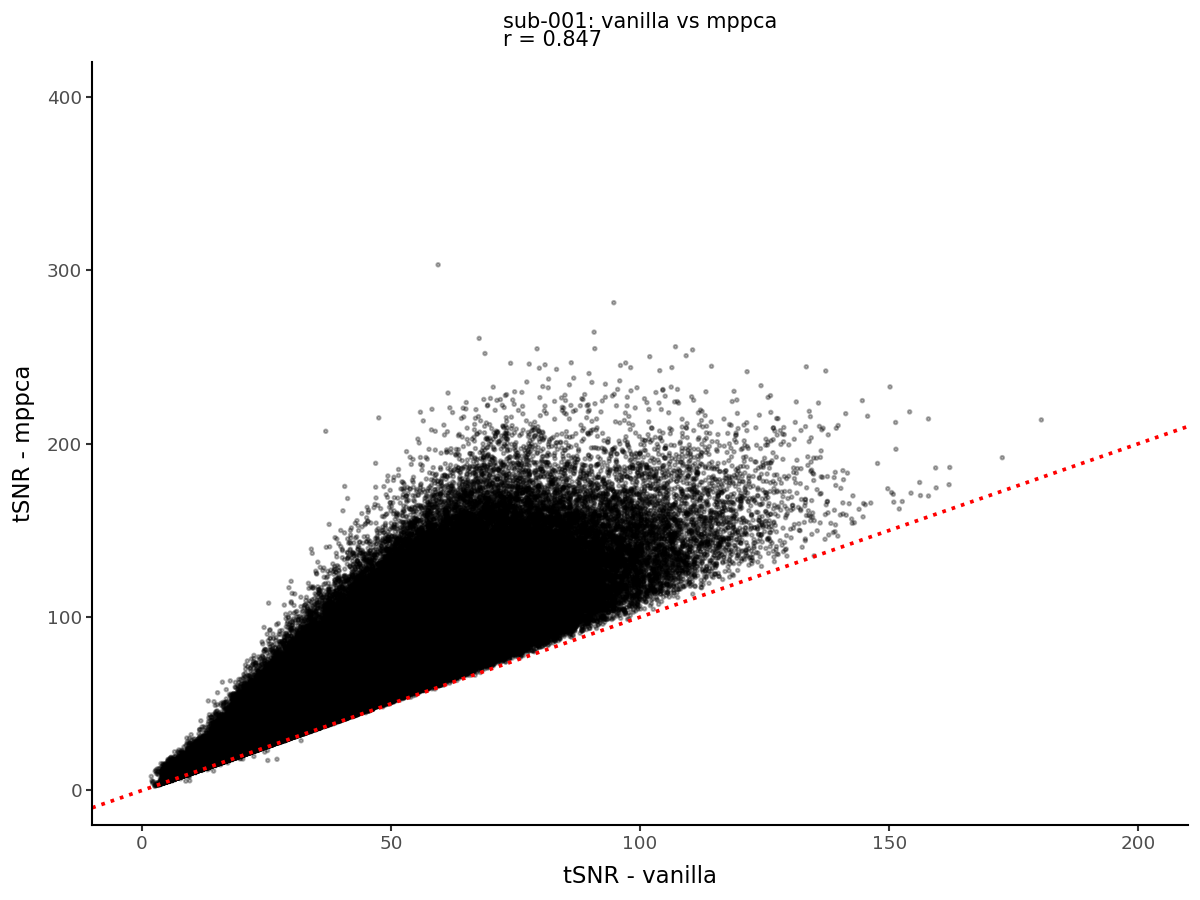
\includegraphics[width=2.5cm]{images/sub-001_vanilla_vs_mppca_tsnr_scatter1700.png}
       & 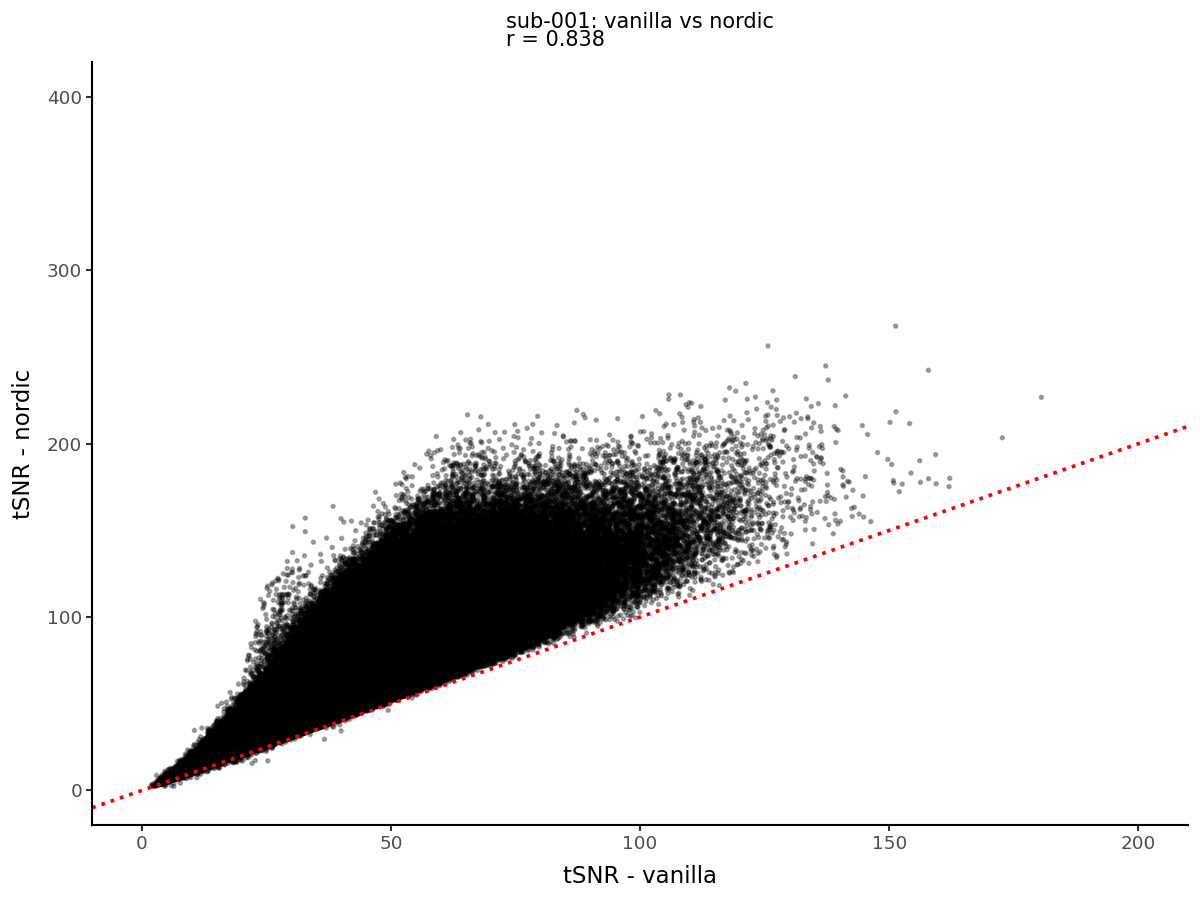
\includegraphics[width=2.5cm]{images/sub-001_vanilla_vs_nordic_tsnr_scatter1700.png}
       & 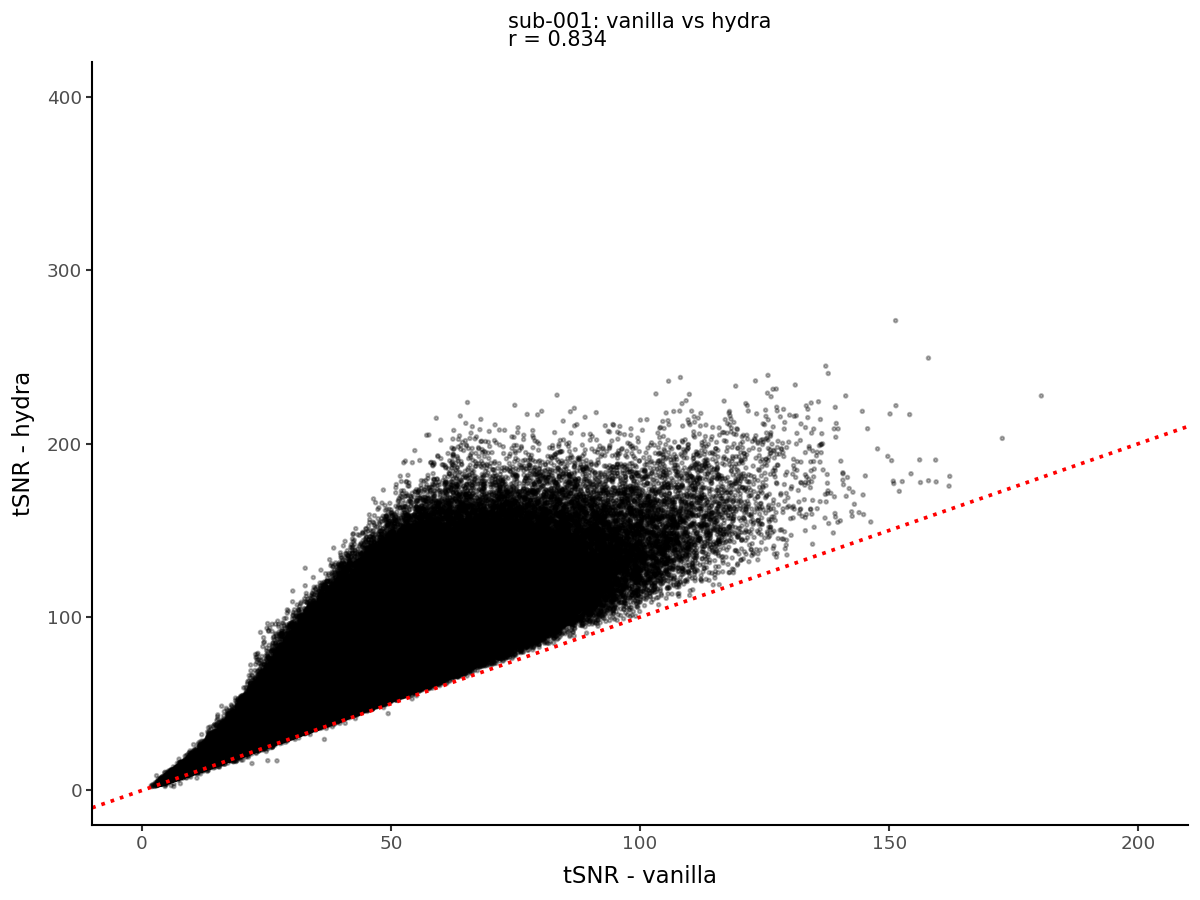
\includegraphics[width=2.5cm]{images/sub-001_vanilla_vs_hydra_tsnr_scatter1700.png}
       & 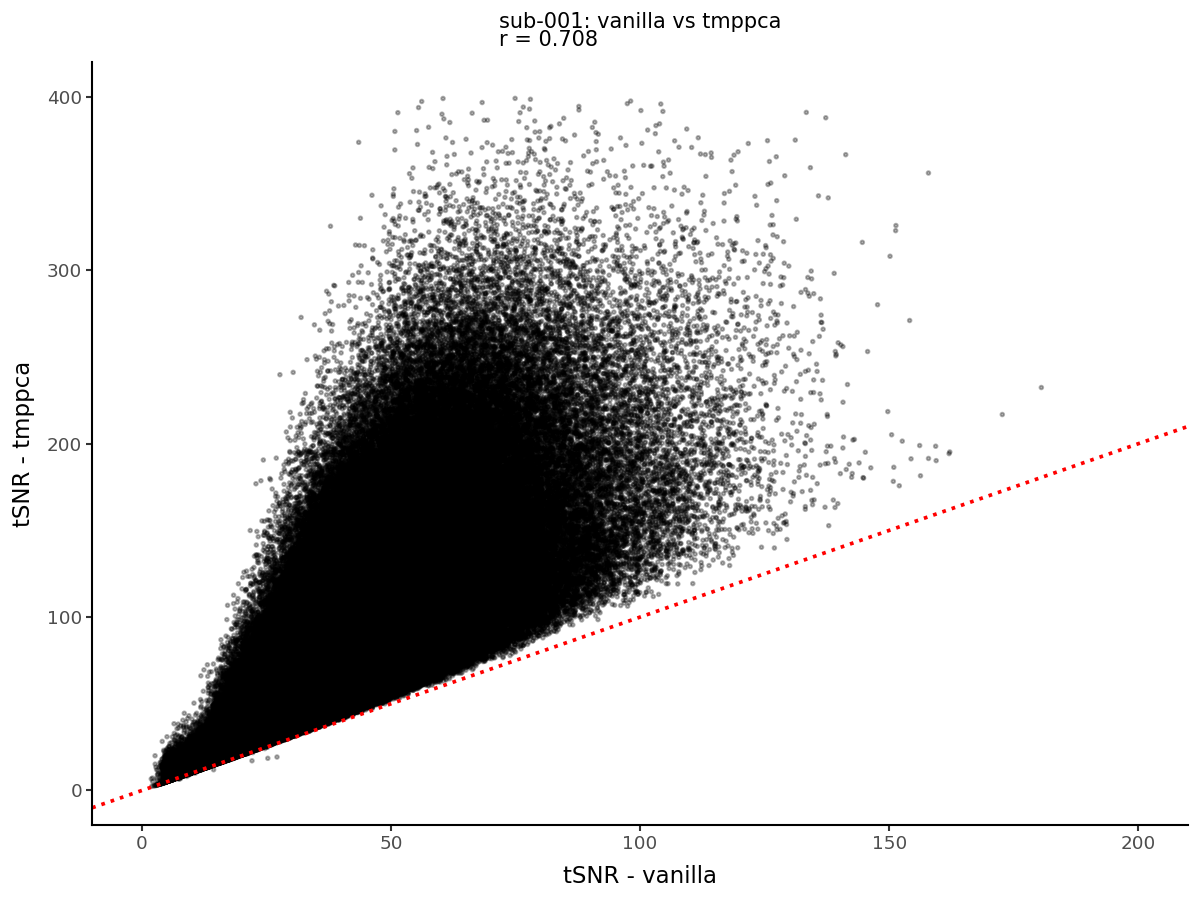
\includegraphics[width=2.5cm]{images/sub-001_vanilla_vs_tmppca_tsnr_scatter1700.png}\\
         \rotatebox[origin=l]{90}{\textcolor{black}{sub-002}}& 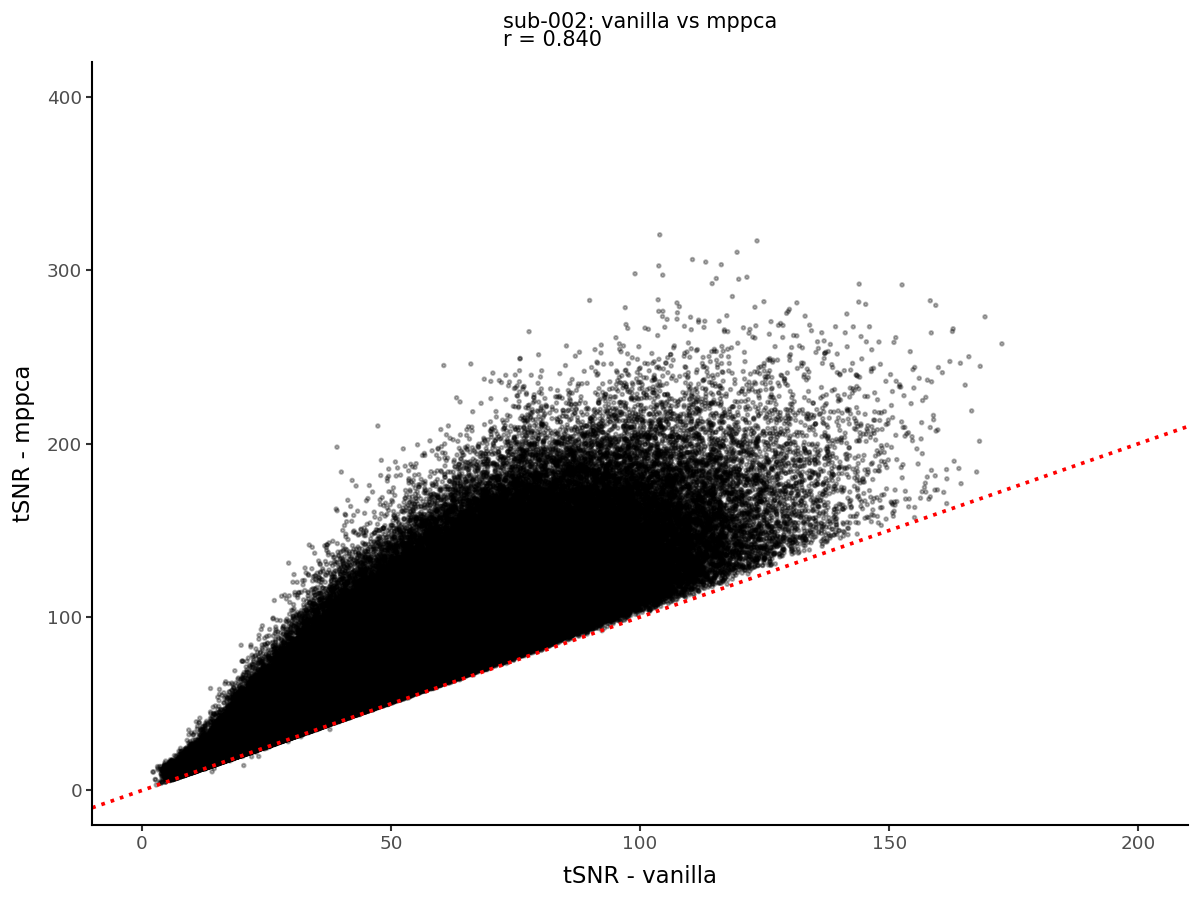
\includegraphics[width=2.5cm]{images/sub-002_vanilla_vs_mppca_tsnr_scatter1700.png}
       & 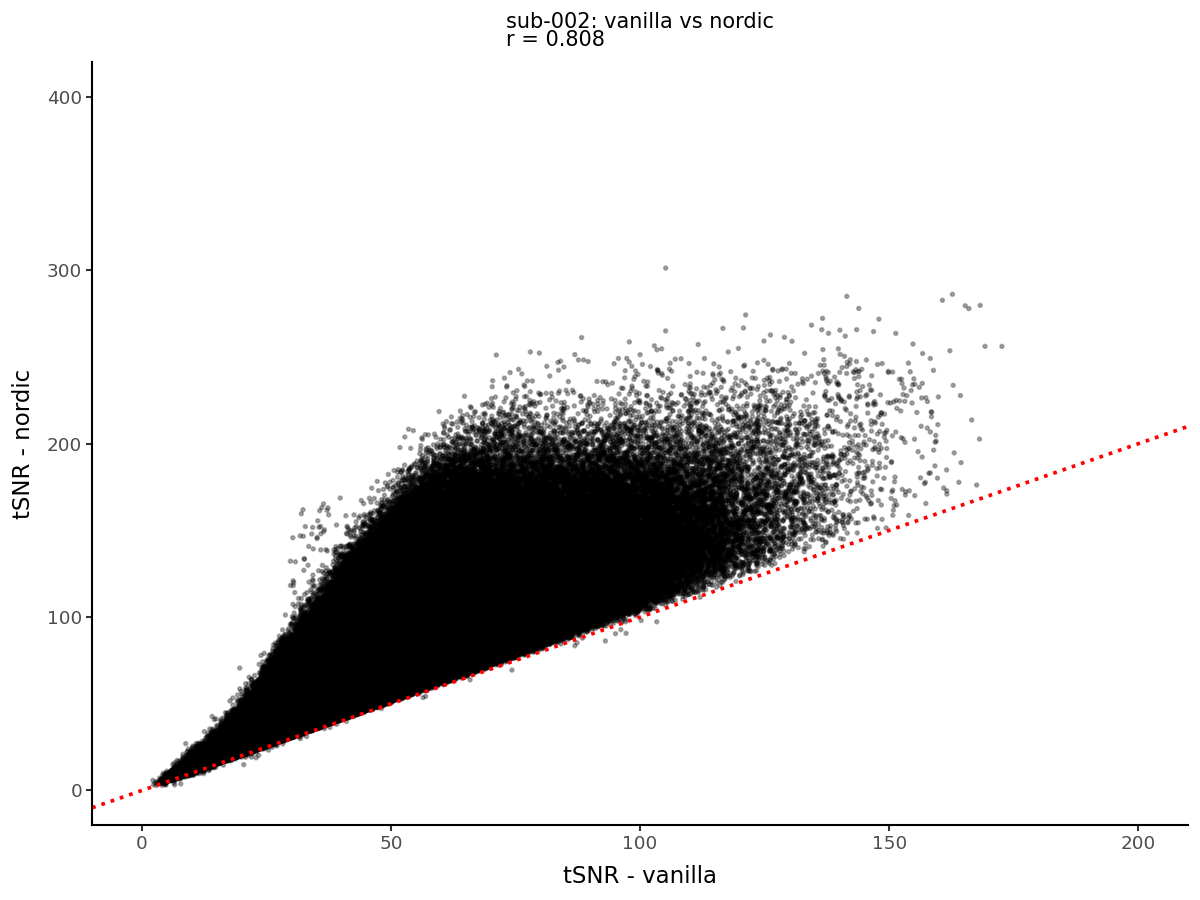
\includegraphics[width=2.5cm]{images/sub-002_vanilla_vs_nordic_tsnr_scatter1700.png}
       & 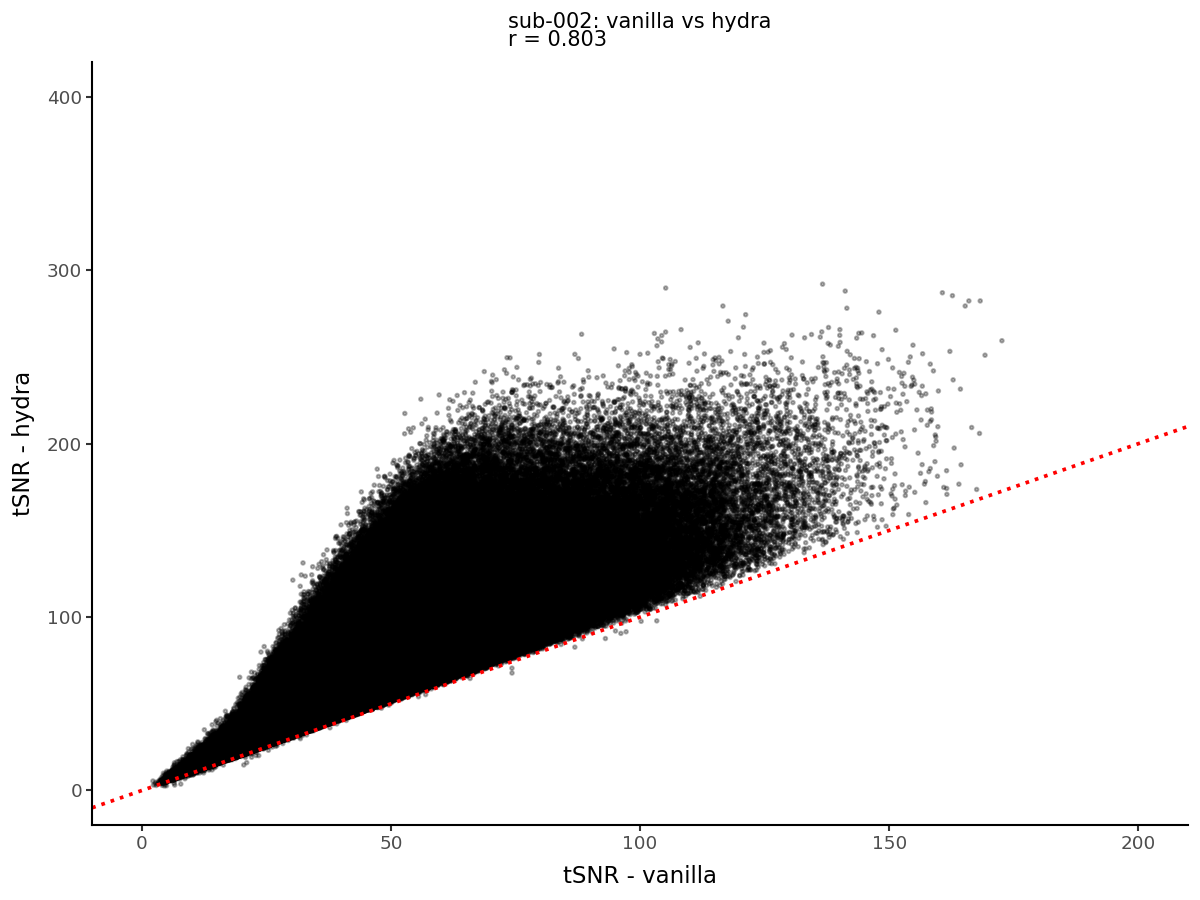
\includegraphics[width=2.5cm]{images/sub-002_vanilla_vs_hydra_tsnr_scatter1700.png}
       & 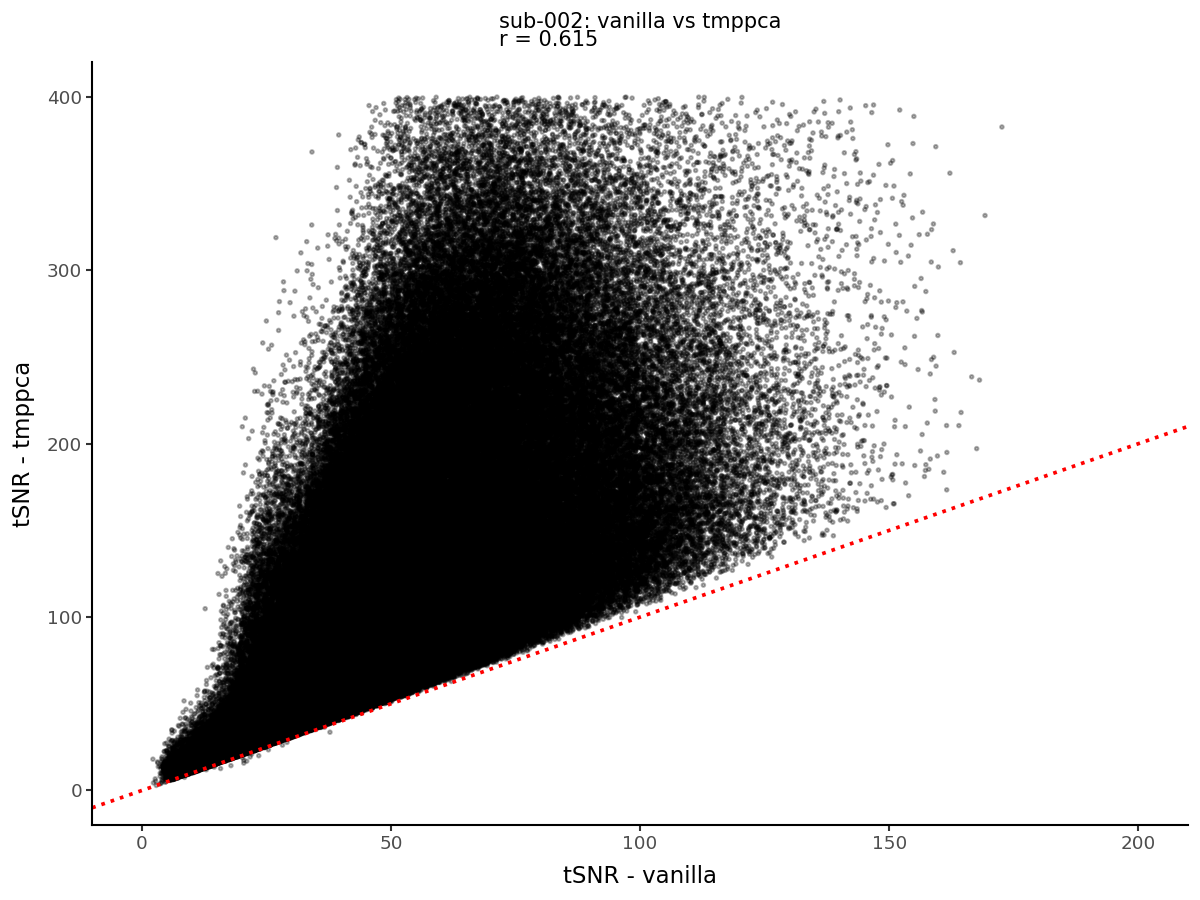
\includegraphics[width=2.5cm]{images/sub-002_vanilla_vs_tmppca_tsnr_scatter1700.png}\\
       \rotatebox[origin=l]{90}{\textcolor{black}{sub-003}}& 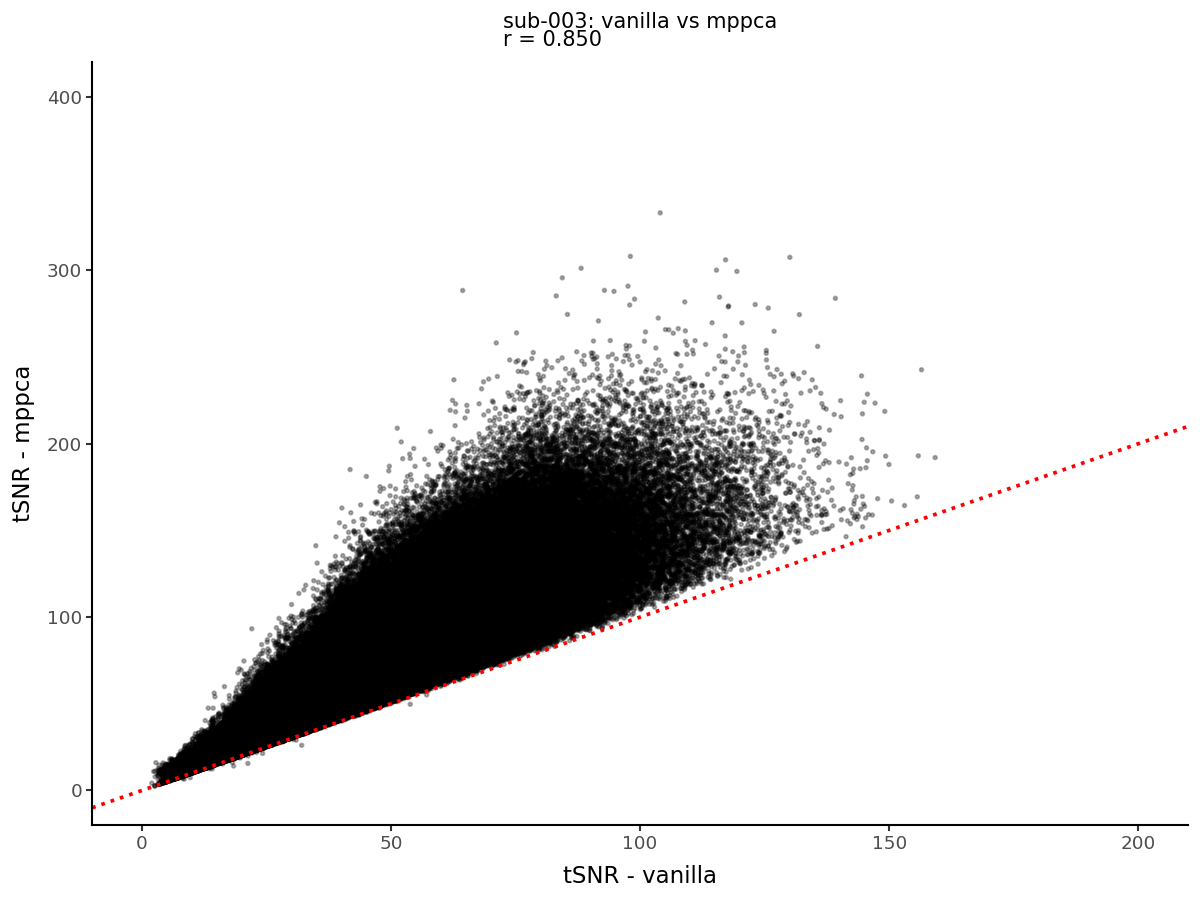
\includegraphics[width=2.5cm]{images/sub-003_vanilla_vs_mppca_tsnr_scatter1700.png}
       & 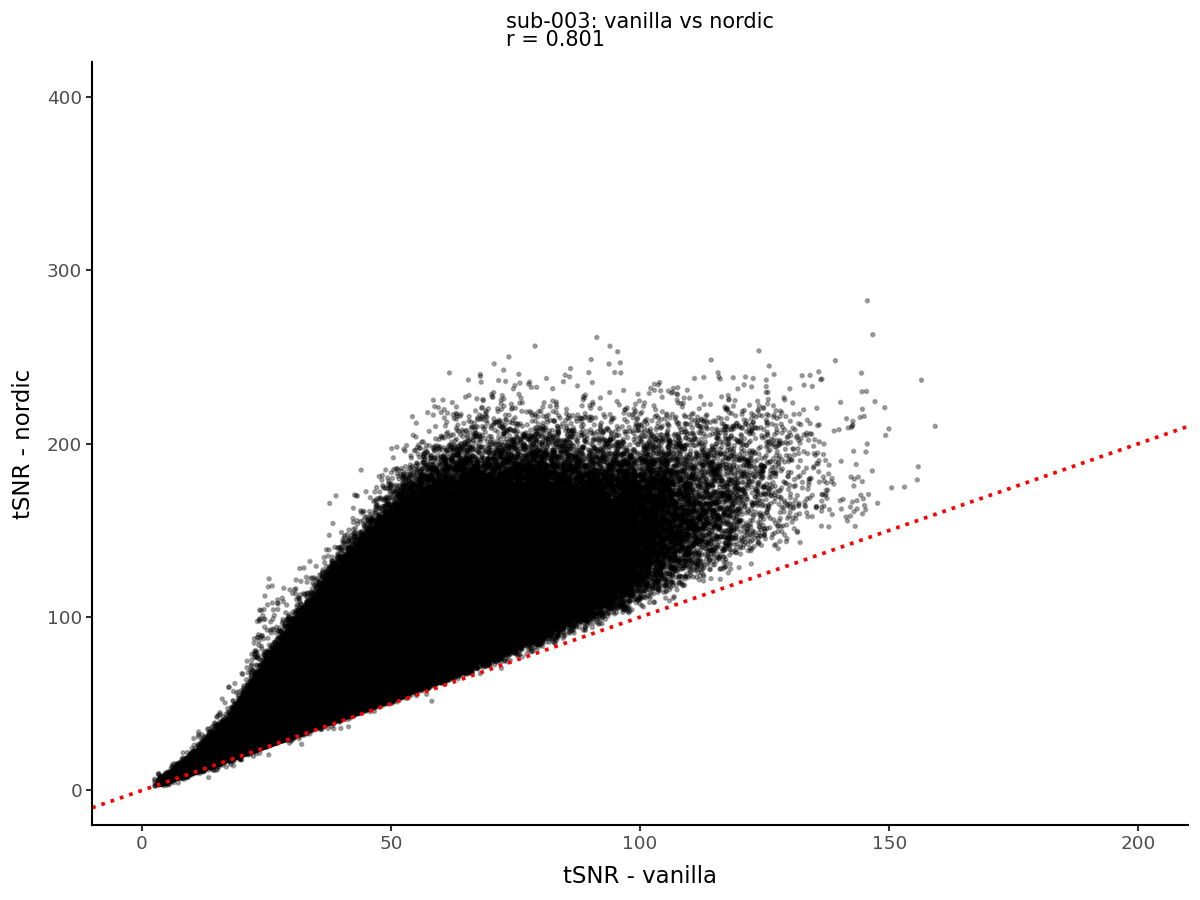
\includegraphics[width=2.5cm]{images/sub-003_vanilla_vs_nordic_tsnr_scatter1700.png}
       & 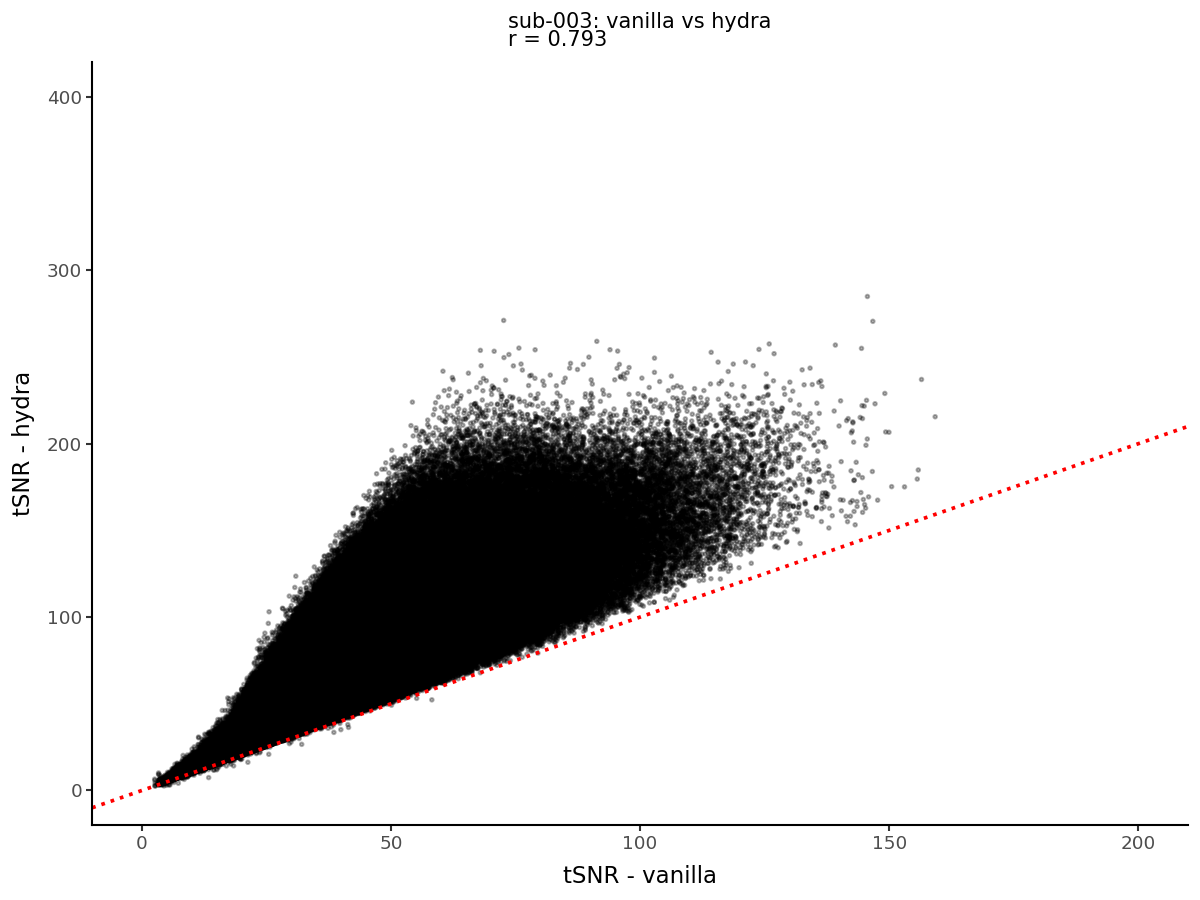
\includegraphics[width=2.5cm]{images/sub-003_vanilla_vs_hydra_tsnr_scatter1700.png}
       & 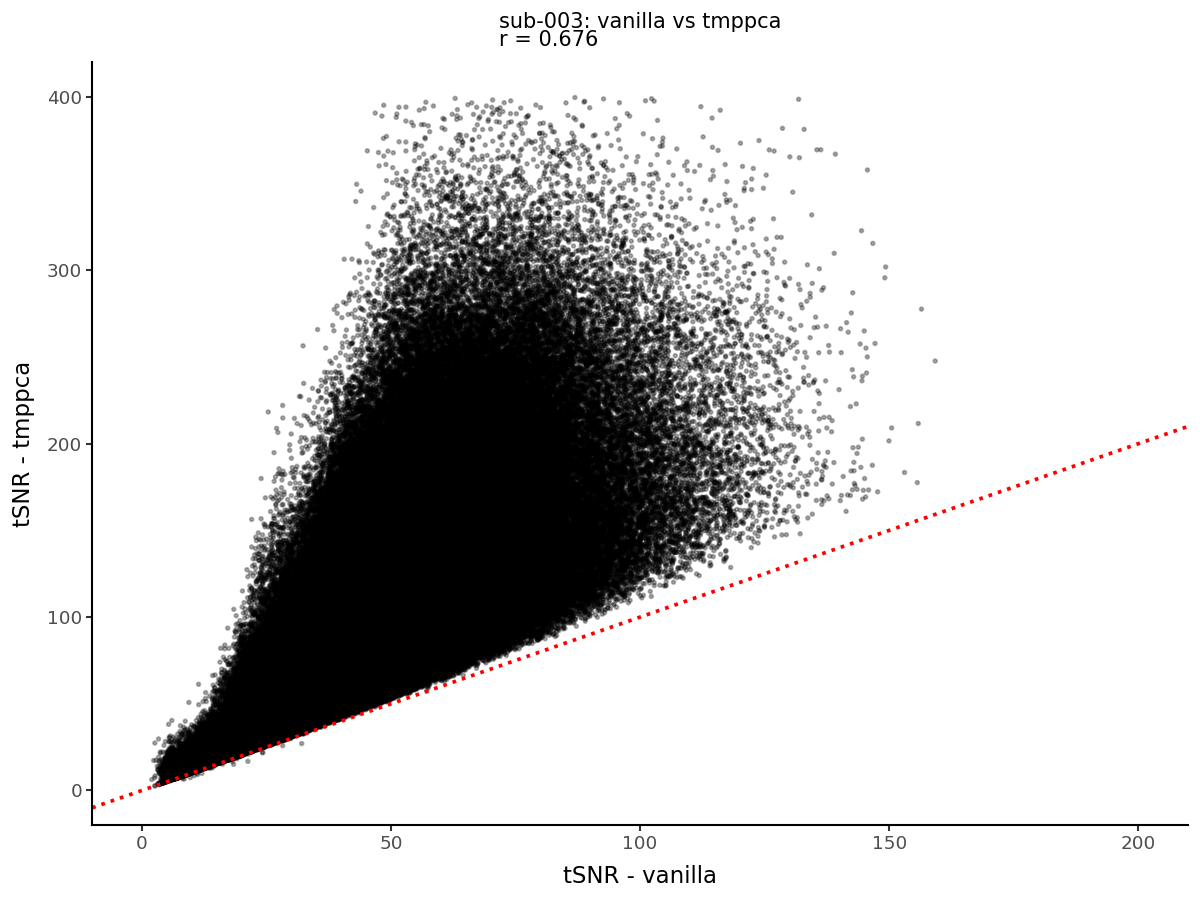
\includegraphics[width=2.5cm]{images/sub-003_vanilla_vs_tmppca_tsnr_scatter1700.png}\\
       
       \rotatebox[origin=l]{90}{\textcolor{black}{sub-004}}& 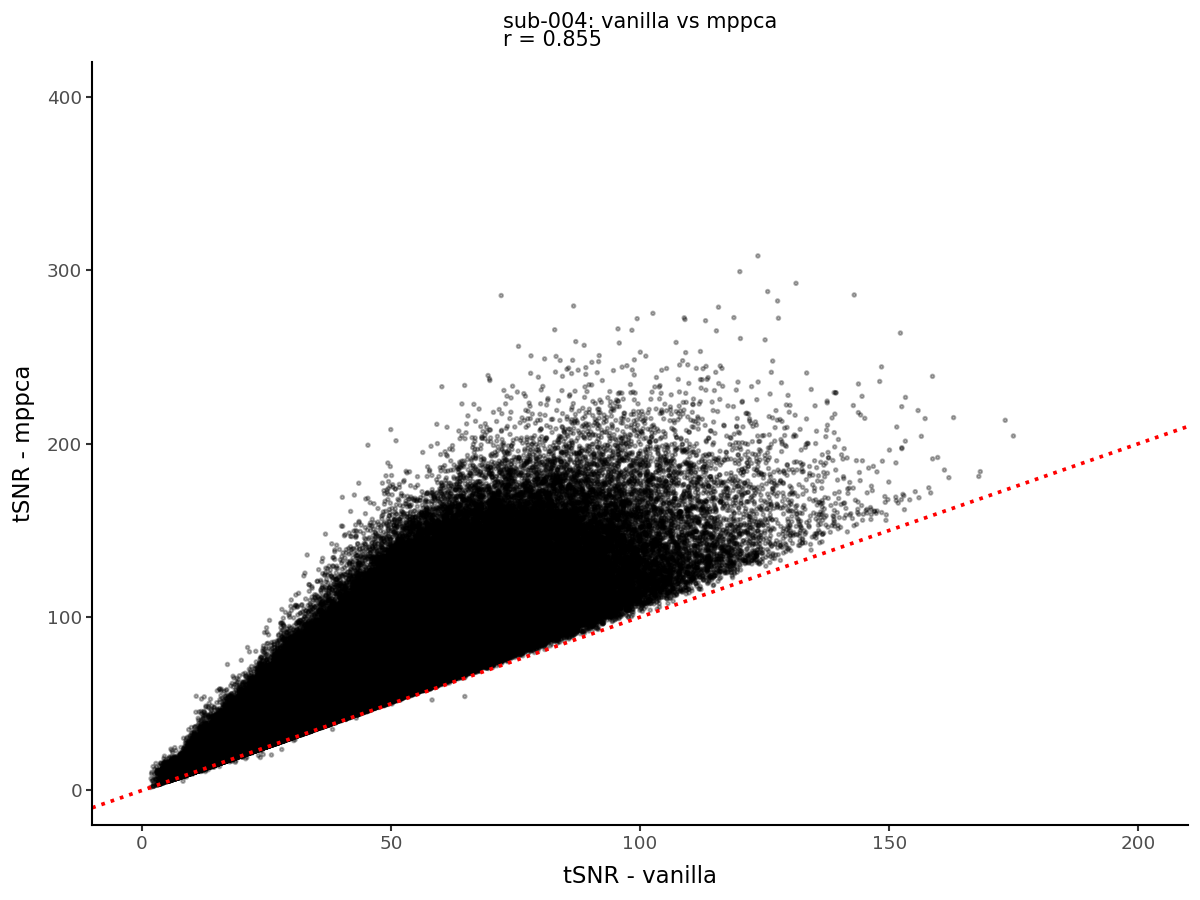
\includegraphics[width=2.5cm]{images/sub-004_vanilla_vs_mppca_tsnr_scatter1700.png}
       & 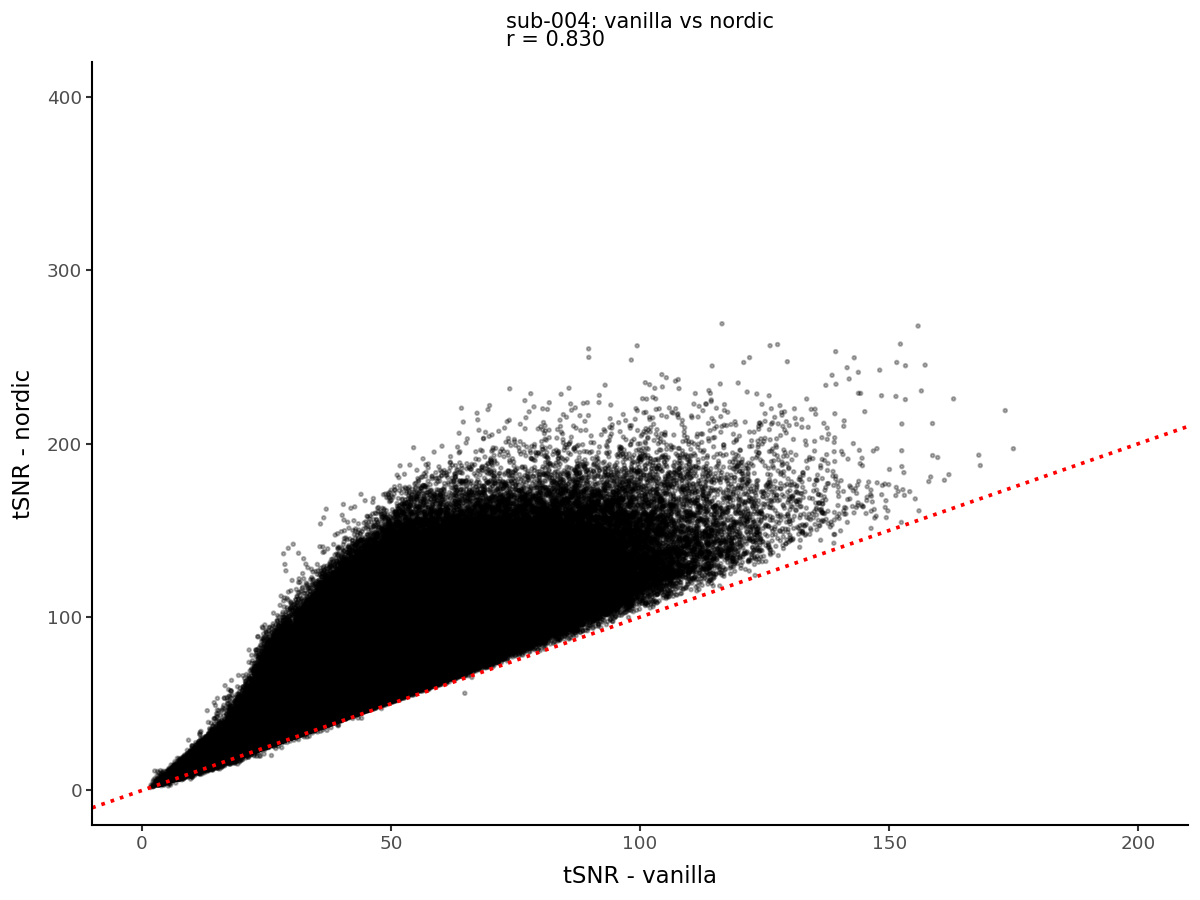
\includegraphics[width=2.5cm]{images/sub-004_vanilla_vs_nordic_tsnr_scatter1700.png}
       & 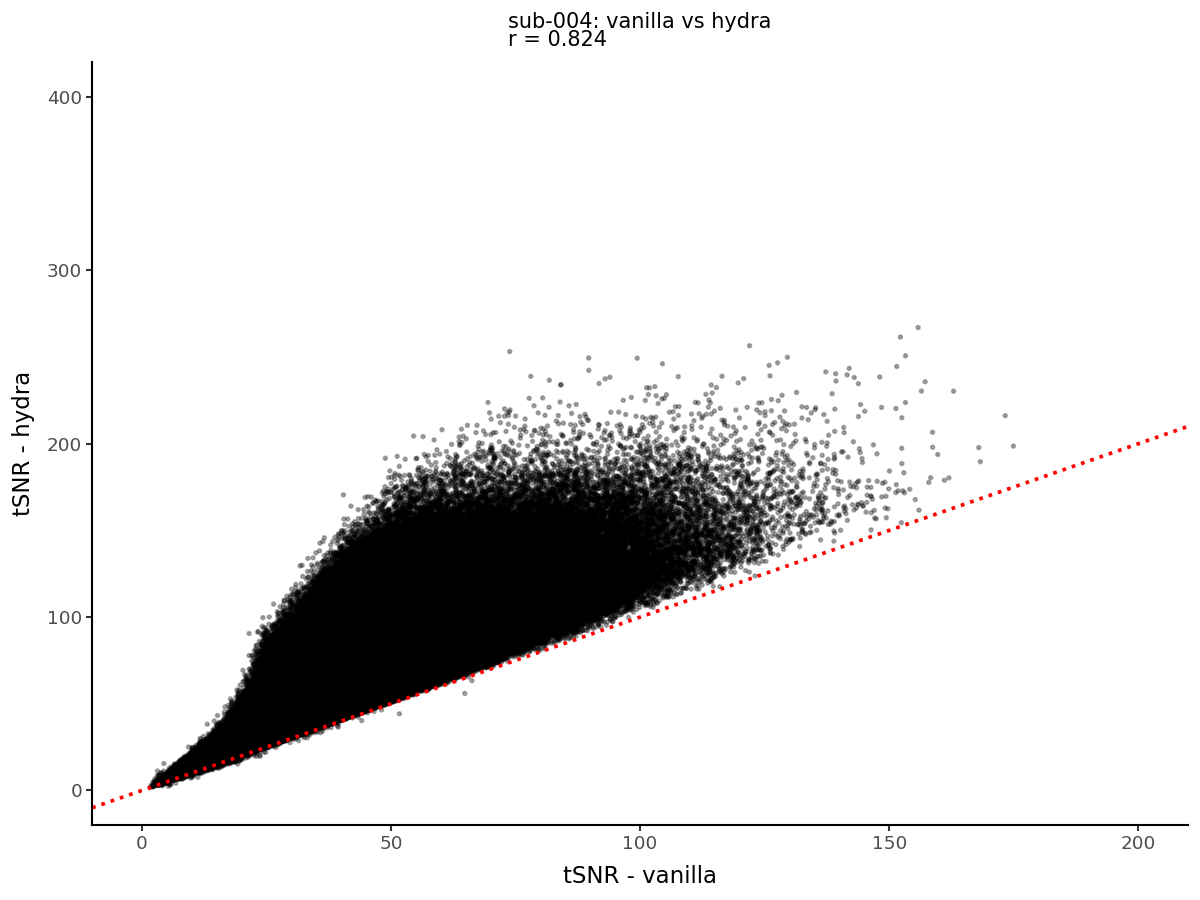
\includegraphics[width=2.5cm]{images/sub-004_vanilla_vs_hydra_tsnr_scatter1700.png}
       & 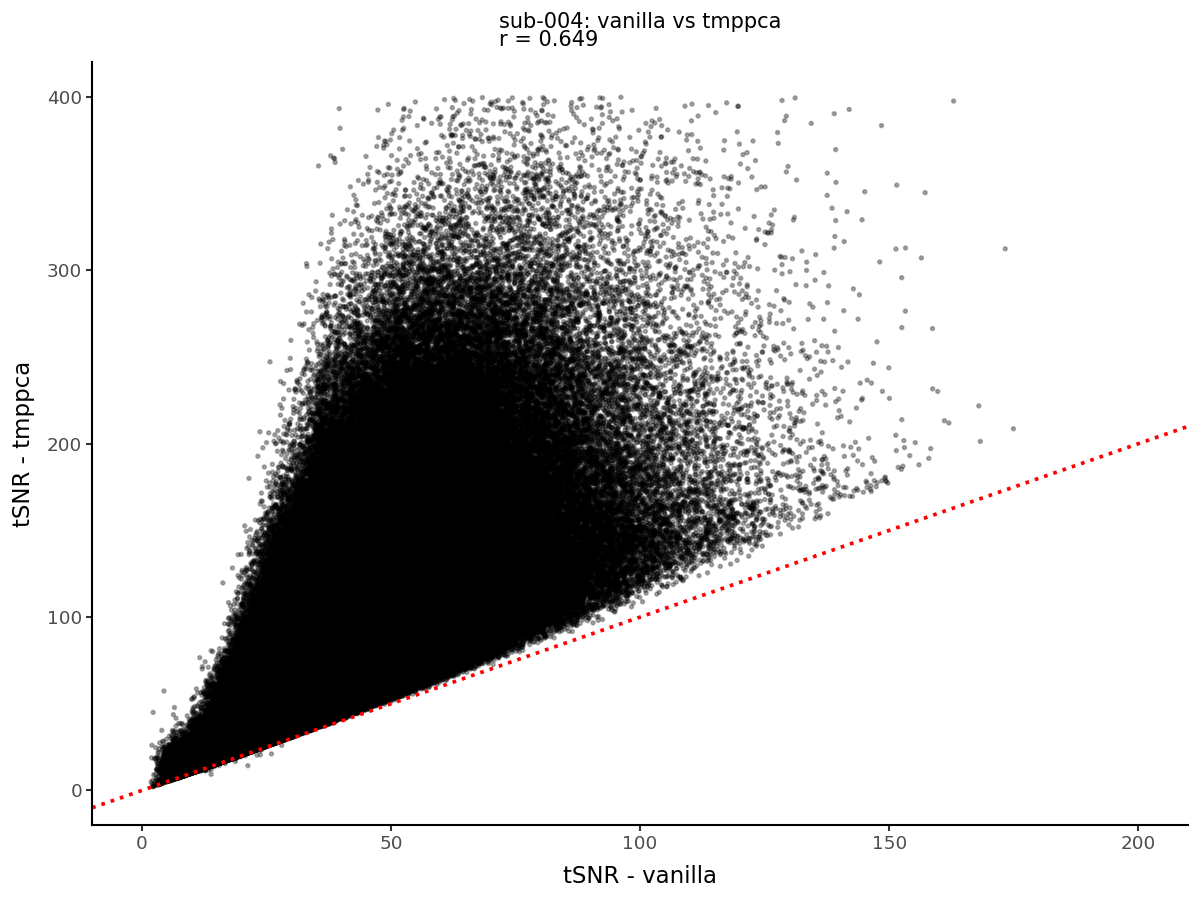
\includegraphics[width=2.5cm]{images/sub-004_vanilla_vs_tmppca_tsnr_scatter1700.png}\\
       \rotatebox[origin=l]{90}{\textcolor{black}{sub-005}}& 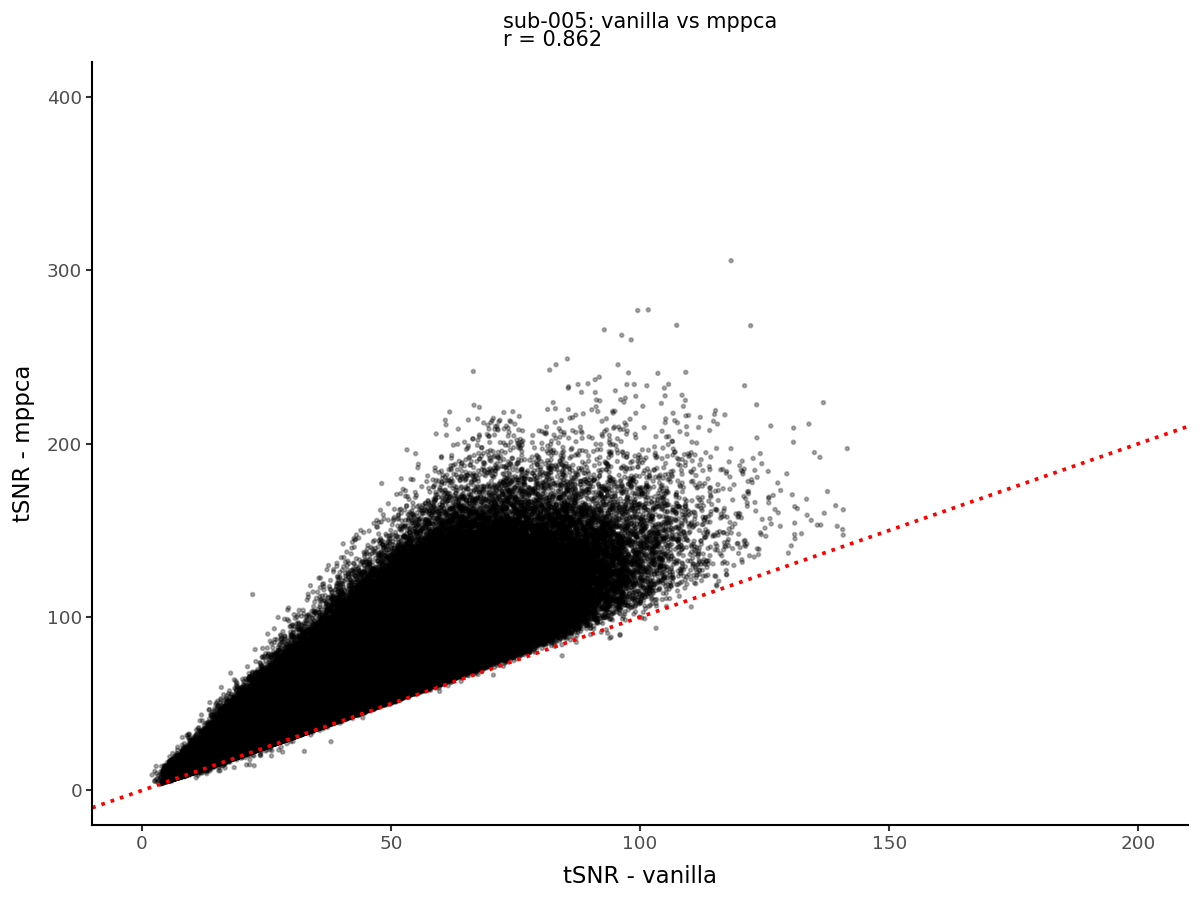
\includegraphics[width=2.5cm]{images/sub-005_vanilla_vs_mppca_tsnr_scatter1700.png}
       & 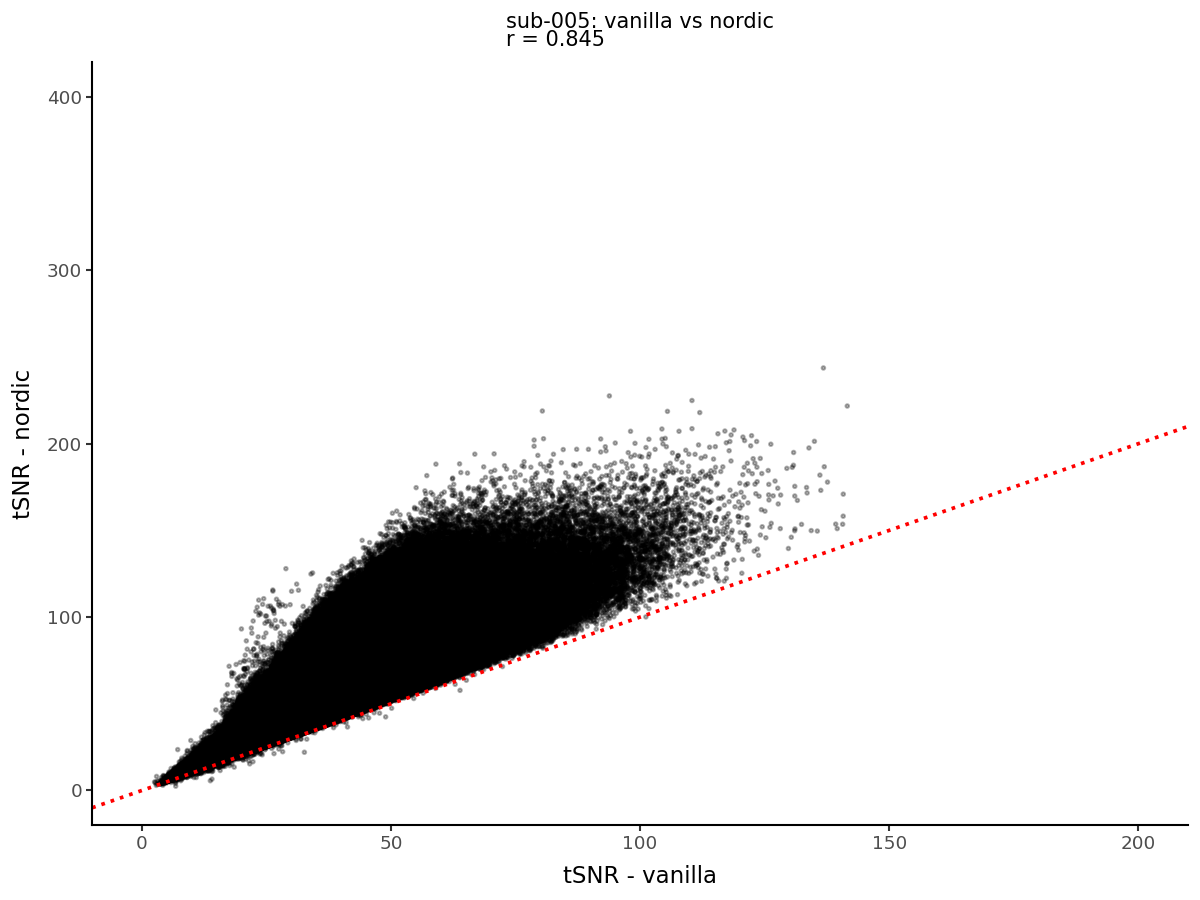
\includegraphics[width=2.5cm]{images/sub-005_vanilla_vs_nordic_tsnr_scatter1700.png}
       & 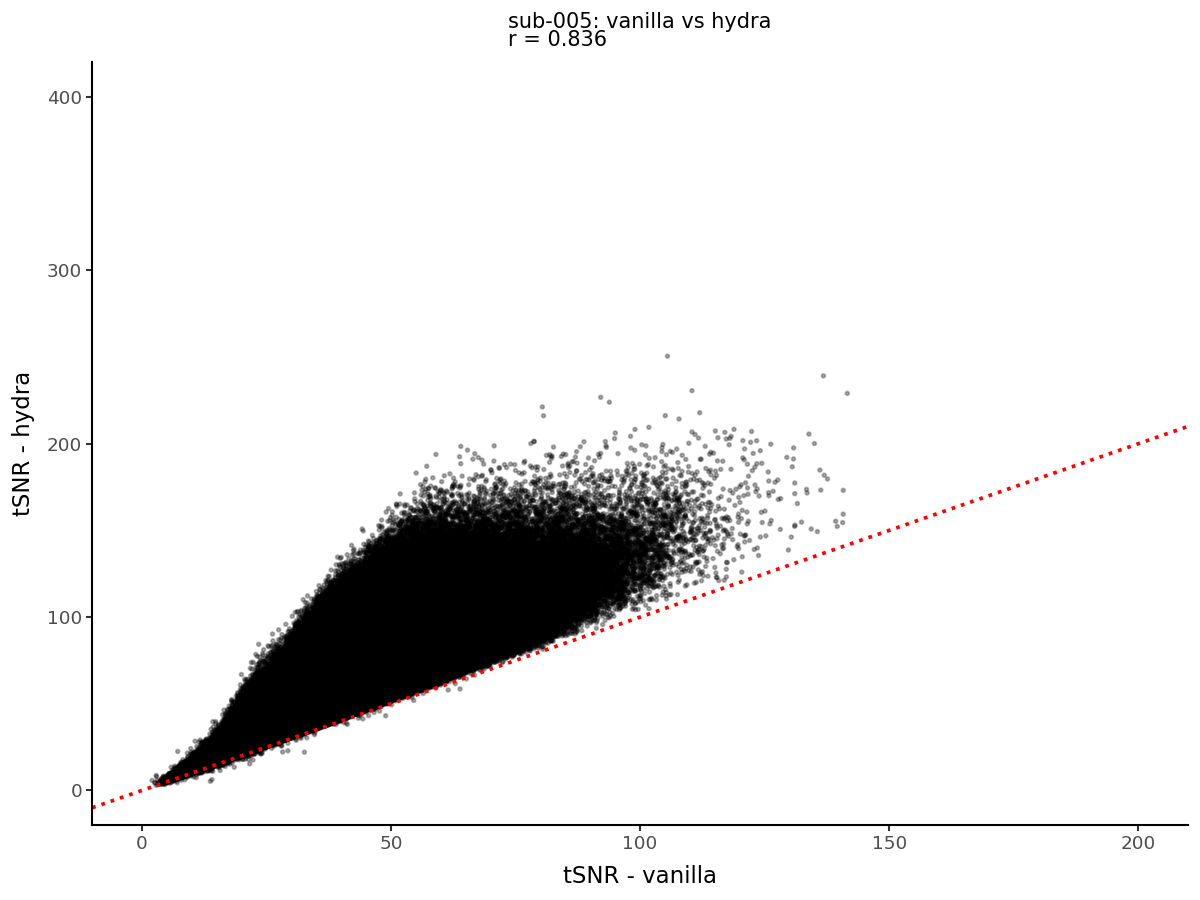
\includegraphics[width=2.5cm]{images/sub-005_vanilla_vs_hydra_tsnr_scatter1700.png}
       & 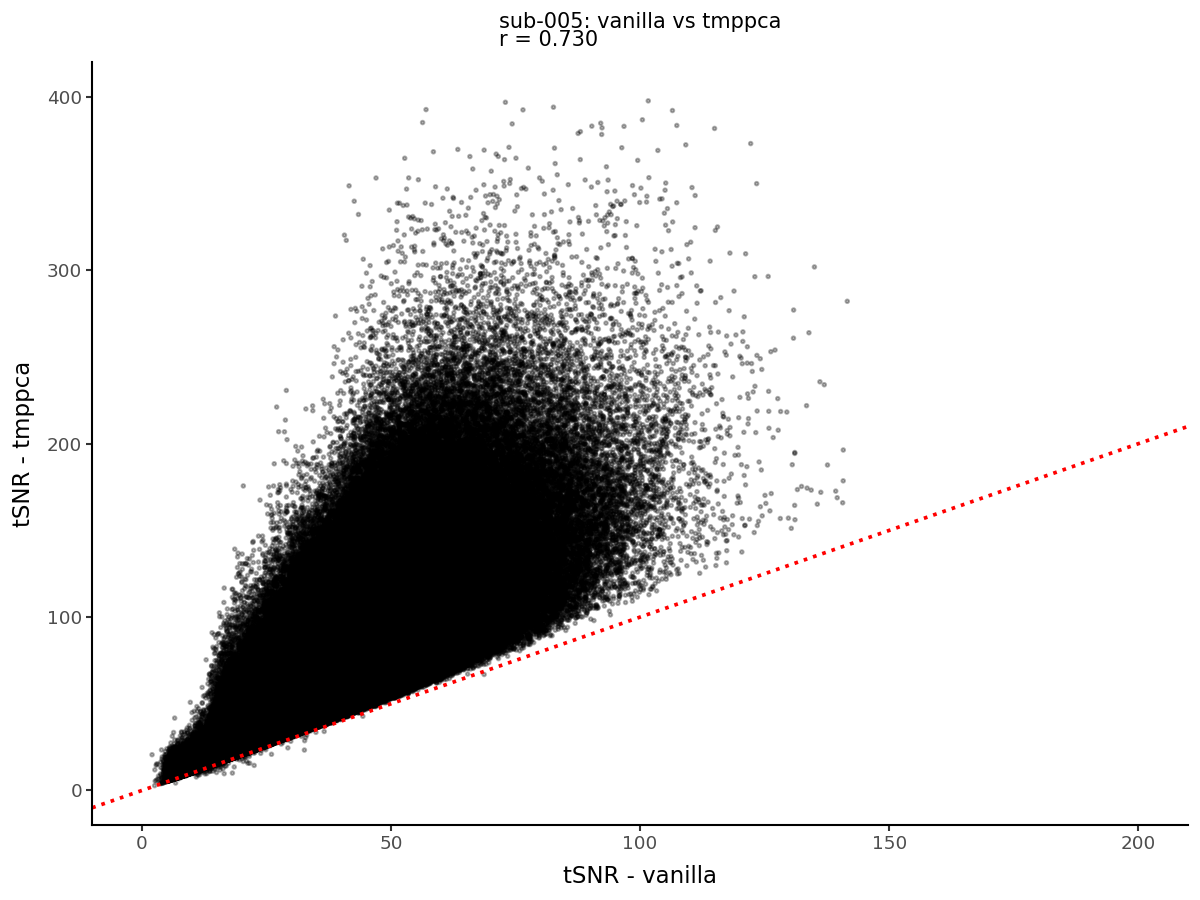
\includegraphics[width=2.5cm]{images/sub-005_vanilla_vs_tmppca_tsnr_scatter1700.png}\\
       \end{tabular}
    }
    \caption[tSNR scatterplots  (2 mm isotropic)]{tSNR scatterplots (2 mm isotropic) comparing vanilla tSNR (x‑axis) versus tSNR after each denoising method (y‑axis). The identity line (red) represents no change.}
    \label{fig:scatter1700}
\end{figure}


\subsubsection{tSNR analysis: high resolution Dataset (1.5 mm) }

%%%%%  -- 1.5 mm -- %%%%%
\begin{figure}[htbp]

\centering
\colorbox{black}{
    \centering
        \begin{tabular}{>{\centering\arraybackslash}m{.5cm}>{\centering\arraybackslash}m{3cm}>{\centering\arraybackslash}m{3cm}>{\centering\arraybackslash}m{.5cm}}
    
       & \textcolor{white}{\textbf{tSNR}} & \textcolor{white}{\textbf{$\Delta tSNR$}}& \\
   \rotatebox[origin=l]{90}{\textcolor{white}{VANILLA}}
  &    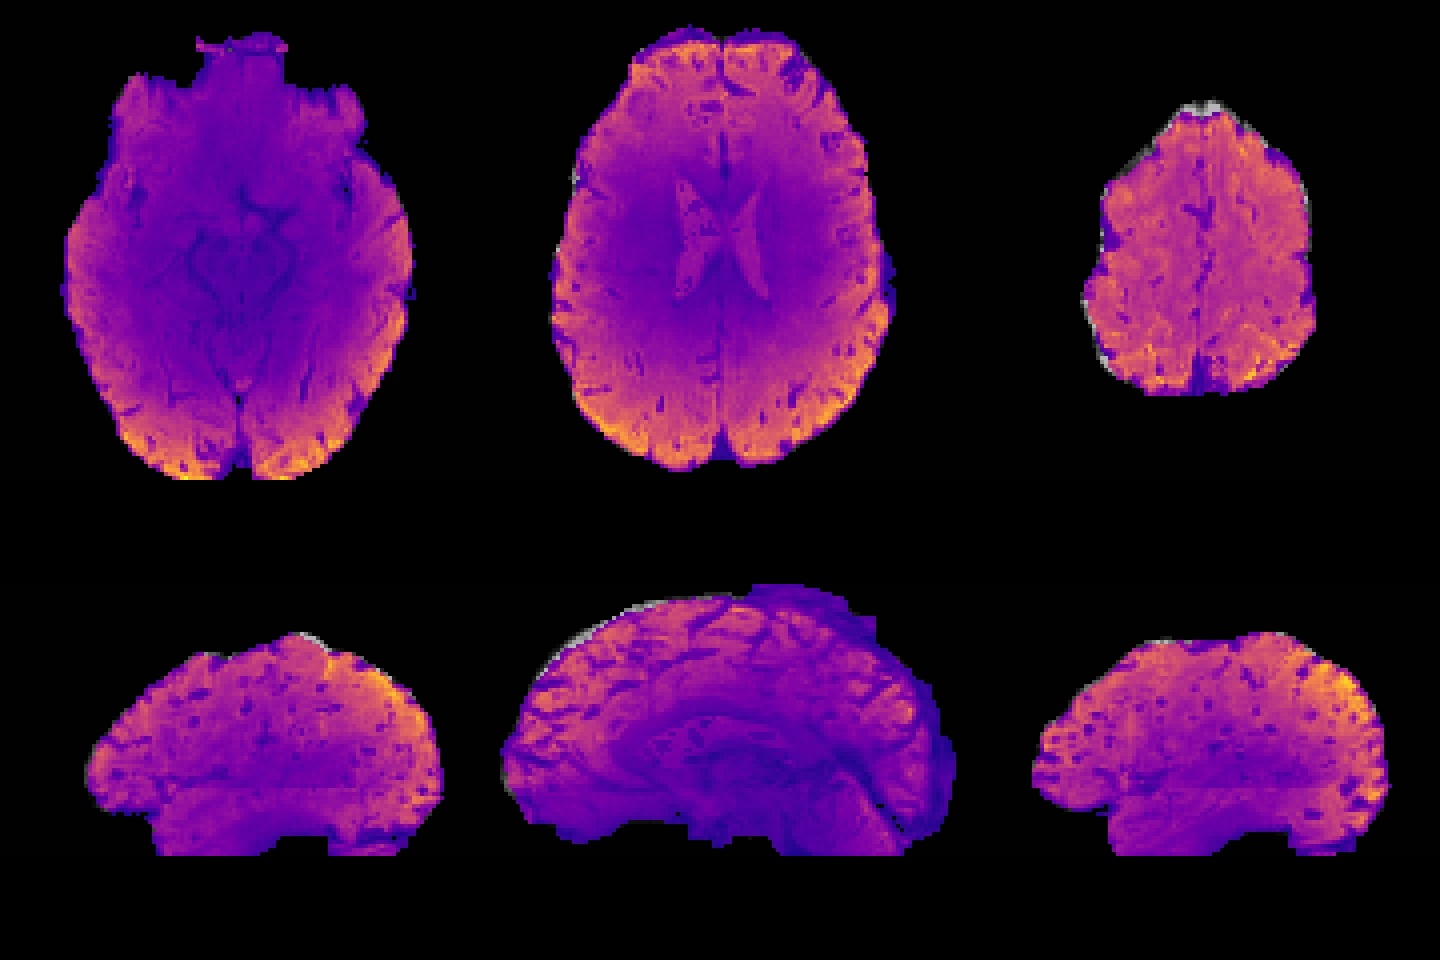
\includegraphics[width=3cm]{images/sub-001_ses-1_task-REST_run-1_OC_part-mag_bold_vanilla_tsnr_all.jpg} & & \textcolor{white}{tSNR} 
\includegraphics[width=.5cm]{images/Plasmatsnr.png}\\
     \rotatebox[origin=l]{90}{\textcolor{white}{MPPCA}}
  &    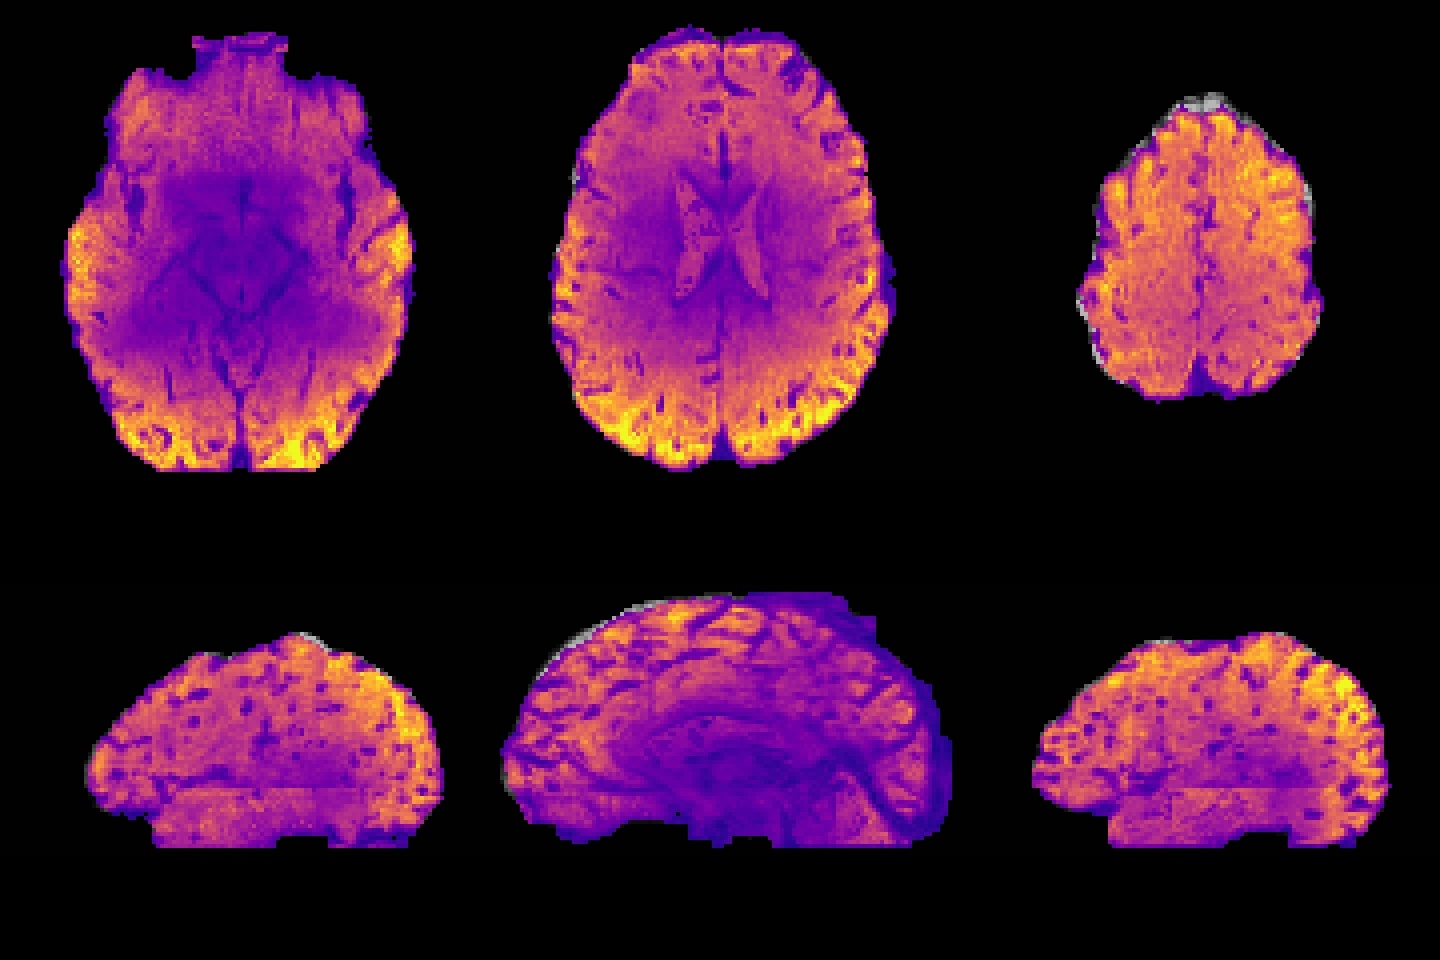
\includegraphics[width=3cm]{images/sub-001_ses-1_task-REST_run-1_OC_part-mag_bold_mppca_tsnr_all.jpg} &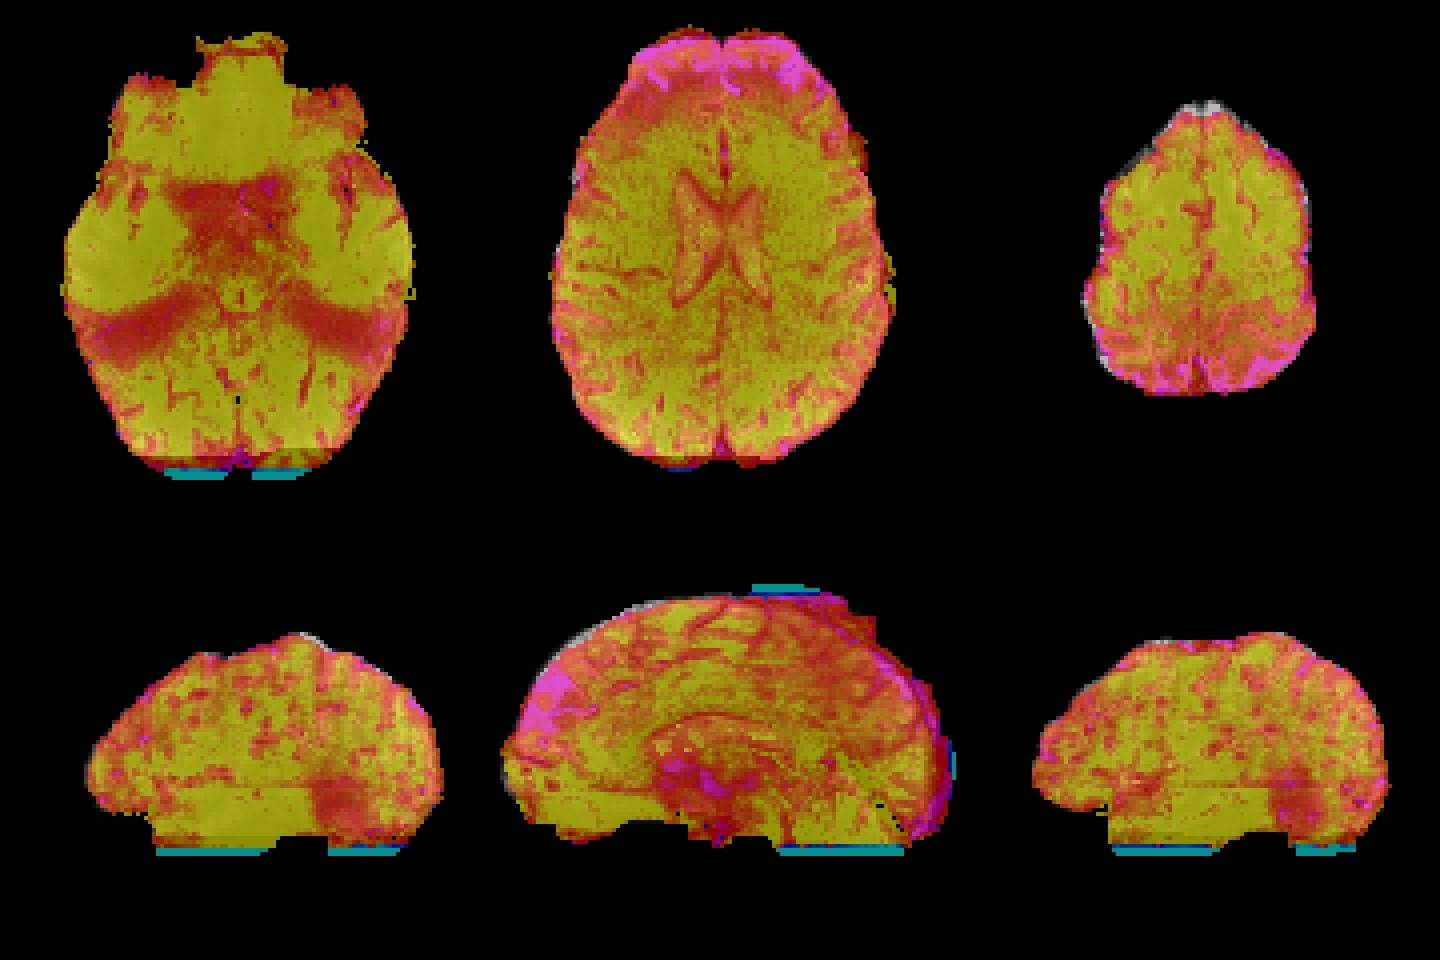
\includegraphics[width=3cm]{images/sub-001_ses-1_task-REST_run-1_OCspc_part-mag_bold_mppca_all} &\\
       \rotatebox[origin=l]{90}{\textcolor{white}{NORDIC}}
  &    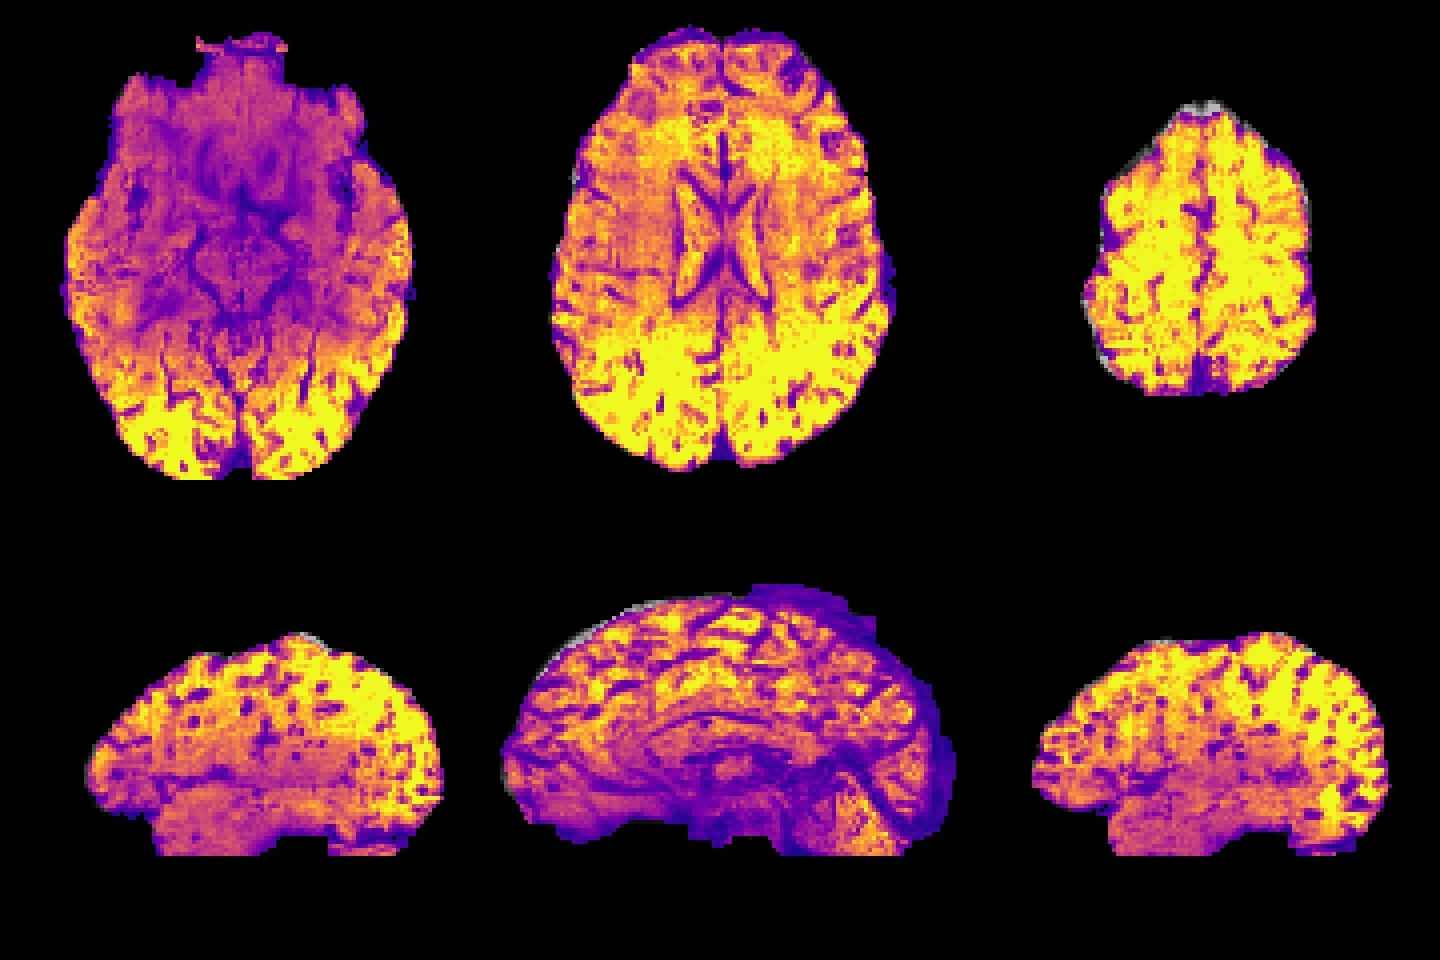
\includegraphics[width=3cm]{images/sub-001_ses-1_task-REST_run-1_OC_part-mag_bold_nordic_tsnr_all.jpg} &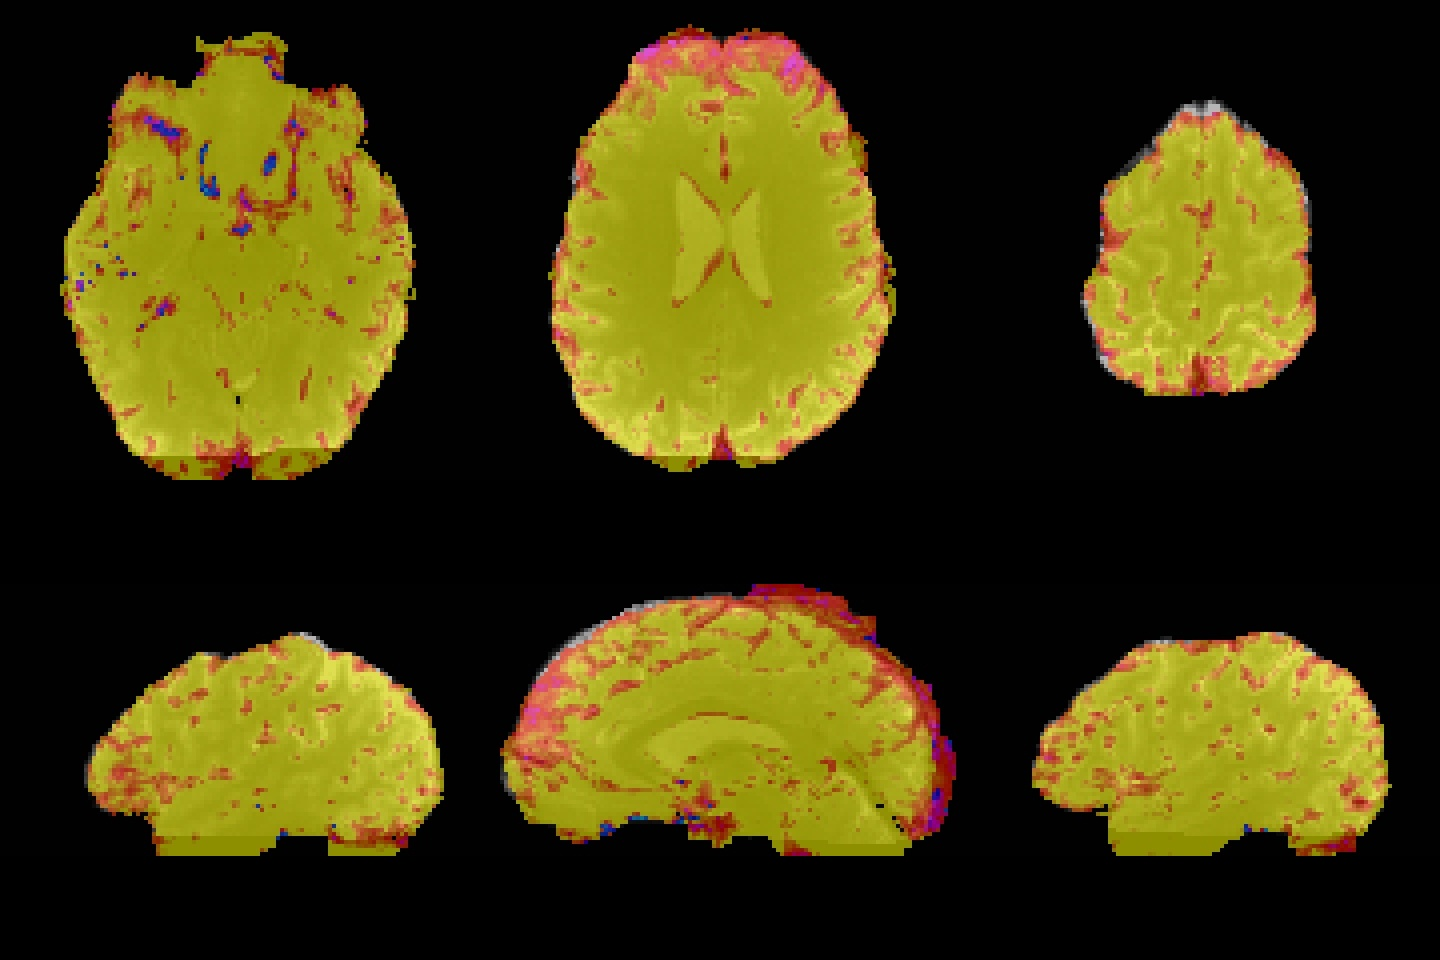
\includegraphics[width=3cm]{images/sub-001_ses-1_task-REST_run-1_OCspc_part-mag_bold_nordic_all} &\\
       \rotatebox[origin=l]{90}{\textcolor{white}{HYDRA}}
  &    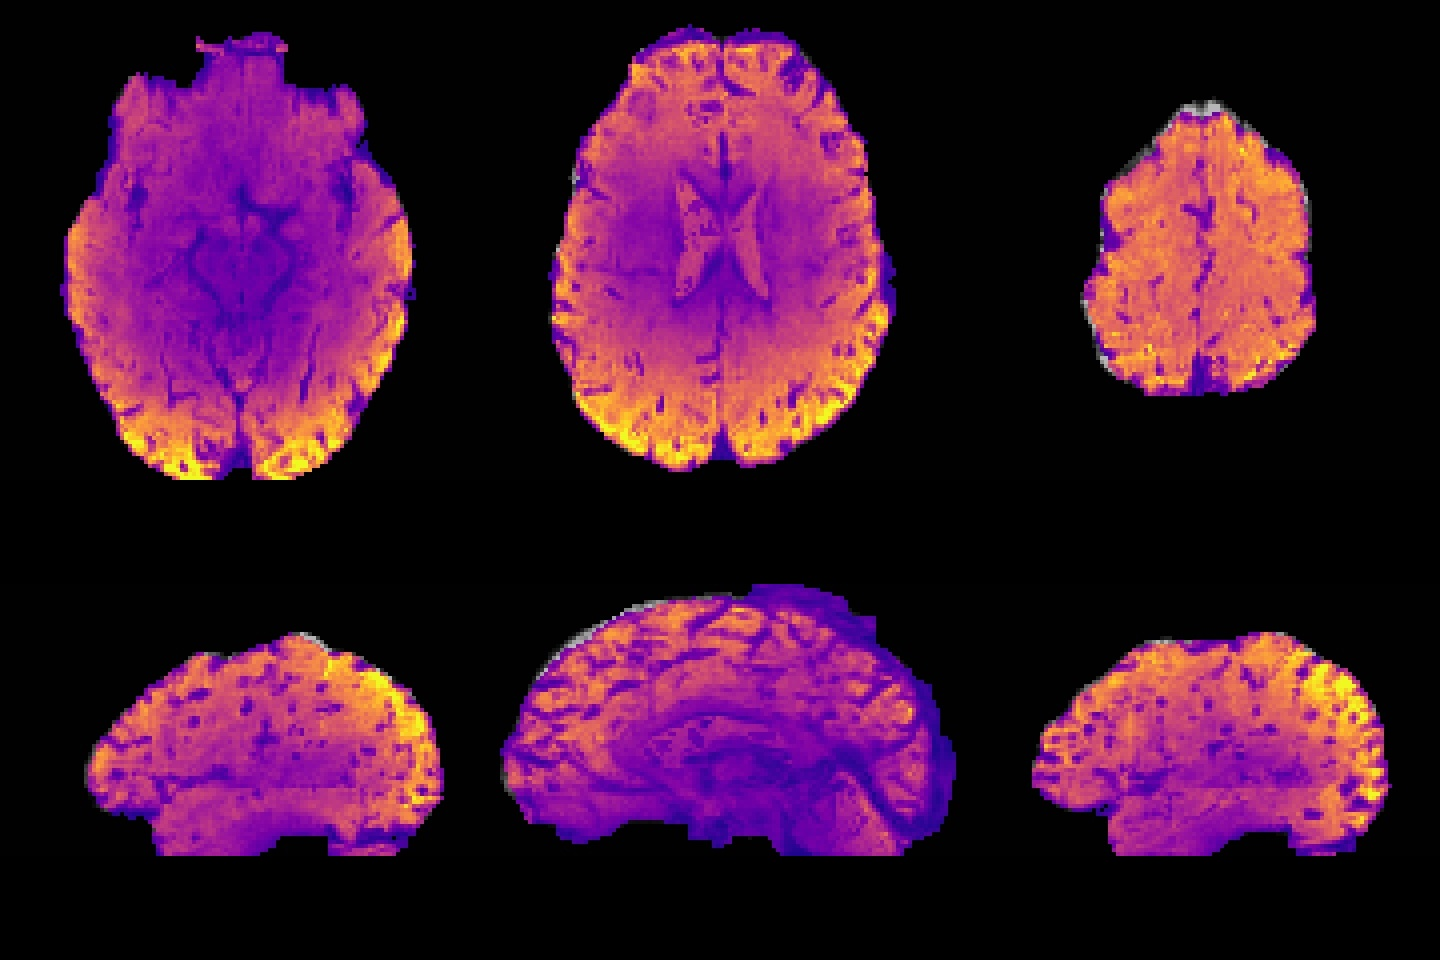
\includegraphics[width=3cm]{images/sub-001_ses-1_task-REST_run-1_OC_part-mag_bold_hydra_tsnr_all.jpg} &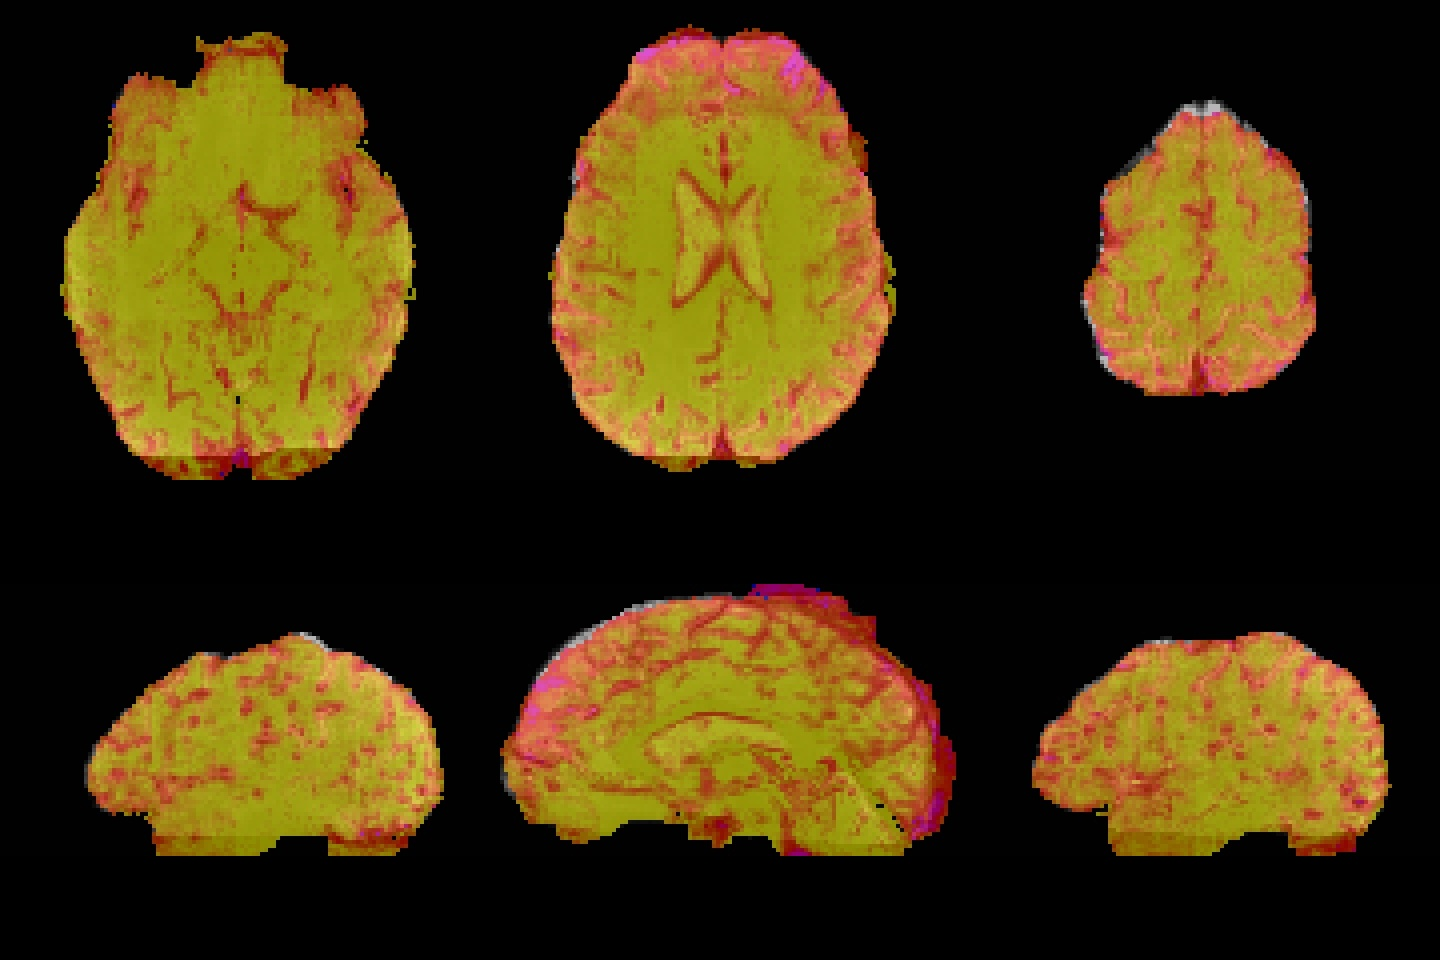
\includegraphics[width=3cm]{images/sub-001_ses-1_task-REST_run-1_OCspc_part-mag_bold_hydra_all} &\\
       \rotatebox[origin=l]{90}{\textcolor{white}{TMPPCA}}
  &    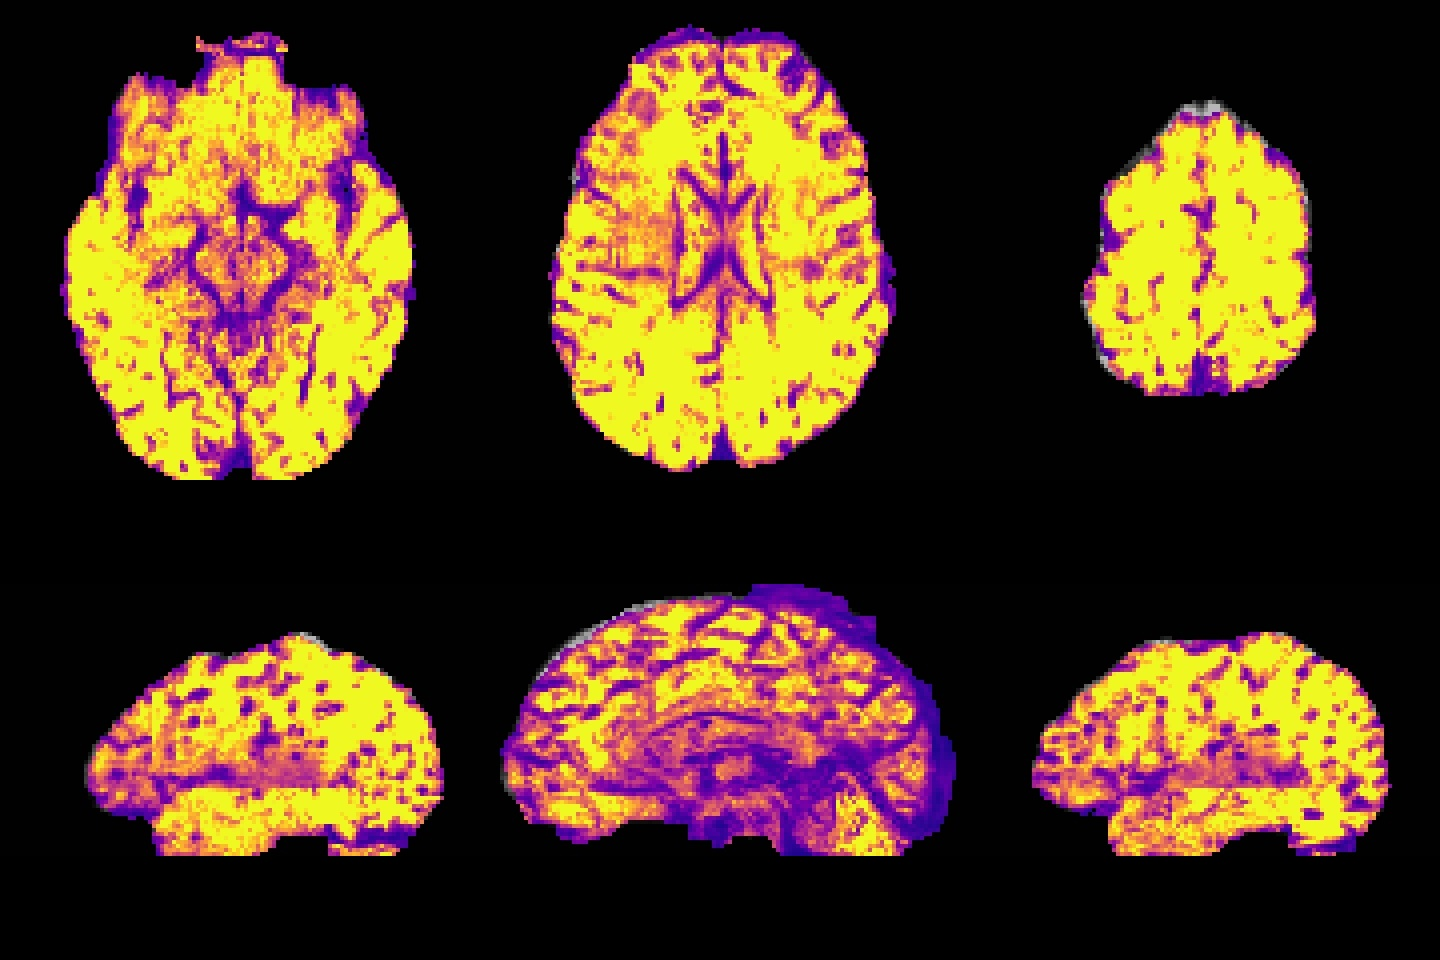
\includegraphics[width=3cm]{images/sub-001_ses-1_task-REST_run-1_OC_part-mag_bold_tmppca_tsnr_all.jpg} &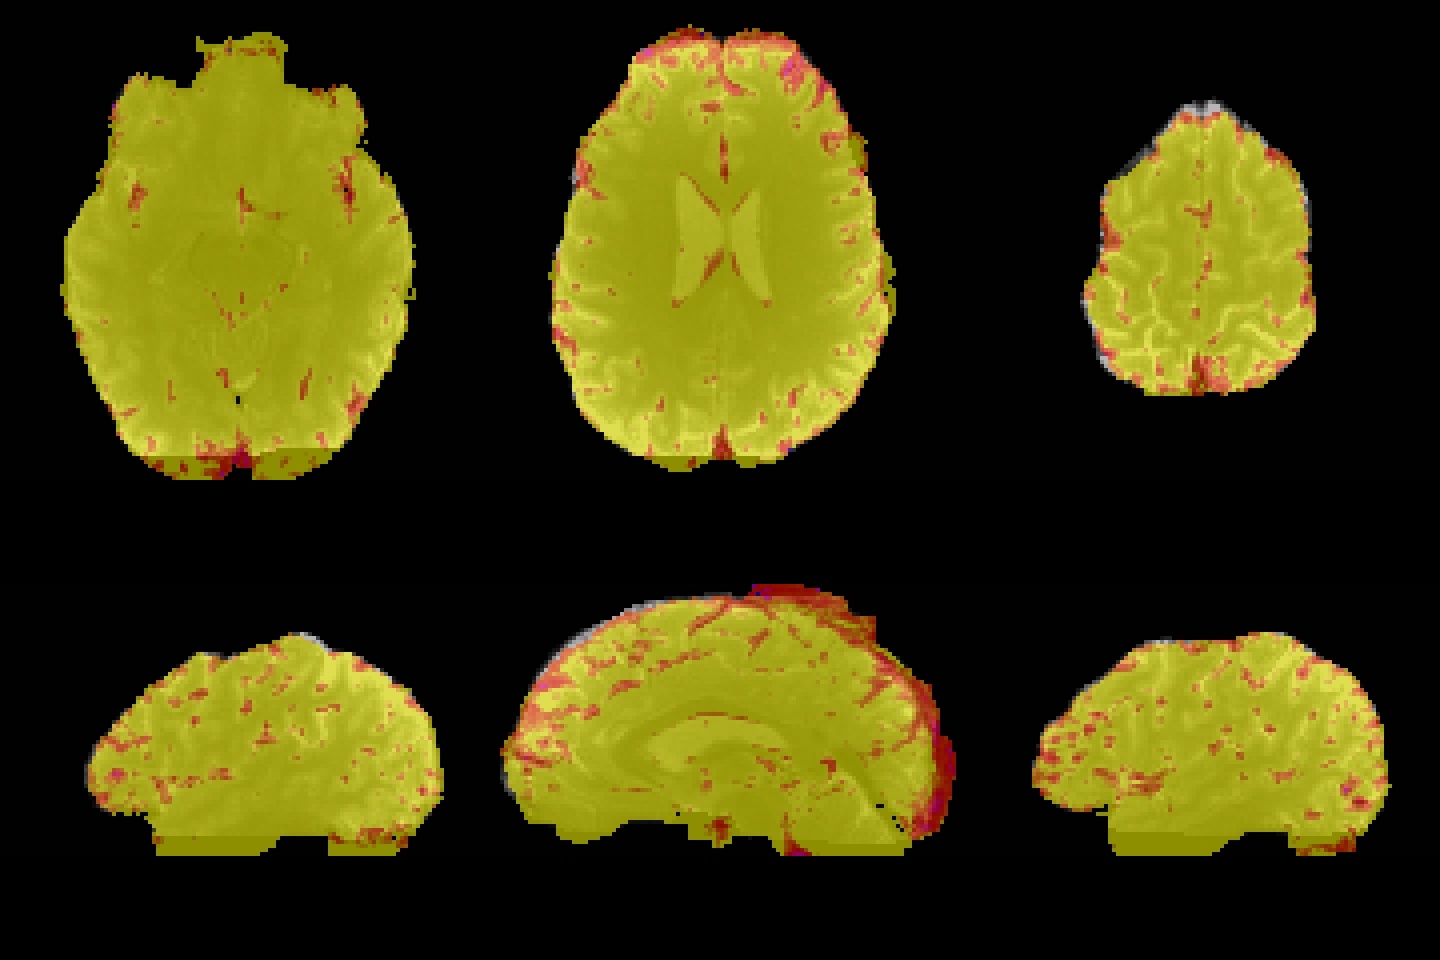
\includegraphics[width=3cm]{images/sub-001_ses-1_task-REST_run-1_OCspc_part-mag_bold_tmppca_all} &\textcolor{white}{$\Delta $} 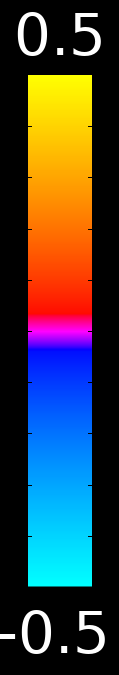
\includegraphics[width=.5cm]{images/SPC.png}\\
    \end{tabular}
    }
    \caption[tSNR  maps, High Resolution (1.5 mm isotropic)]{tSNR analysis at 1.5 mm (saturation limit 100 a.u.). Left: tSNR maps. Right: $\Delta$tSNR maps (change relative to vanilla).}
    \label{fig:tsnrHR}
\end{figure}

%-- scatterplot
\begin{figure}[htbp]
\raggedright
\captionsetup{justification=raggedleft,singlelinecheck=off}\colorbox{white}{
    \raggedleft
    \begin{tabular}{>{\raggedright\arraybackslash}m{.5cm}>{\raggedright\arraybackslash}m{2.5cm}>{\raggedright\arraybackslash}m{2.5cm}>{\raggedright\arraybackslash}m{2.5cm}>{\raggedright\arraybackslash}m{2.5cm}}
       & \textcolor{black}{\textbf{MPPCA}}
       & \textcolor{black}{\textbf{NORDIC}}
       & \textcolor{black}{\textbf{HYDRA}}
       & \textcolor{black}{\textbf{TMPPCA}}\\
       \rotatebox[origin=l]{90}{\textcolor{black}{sub-001}}& 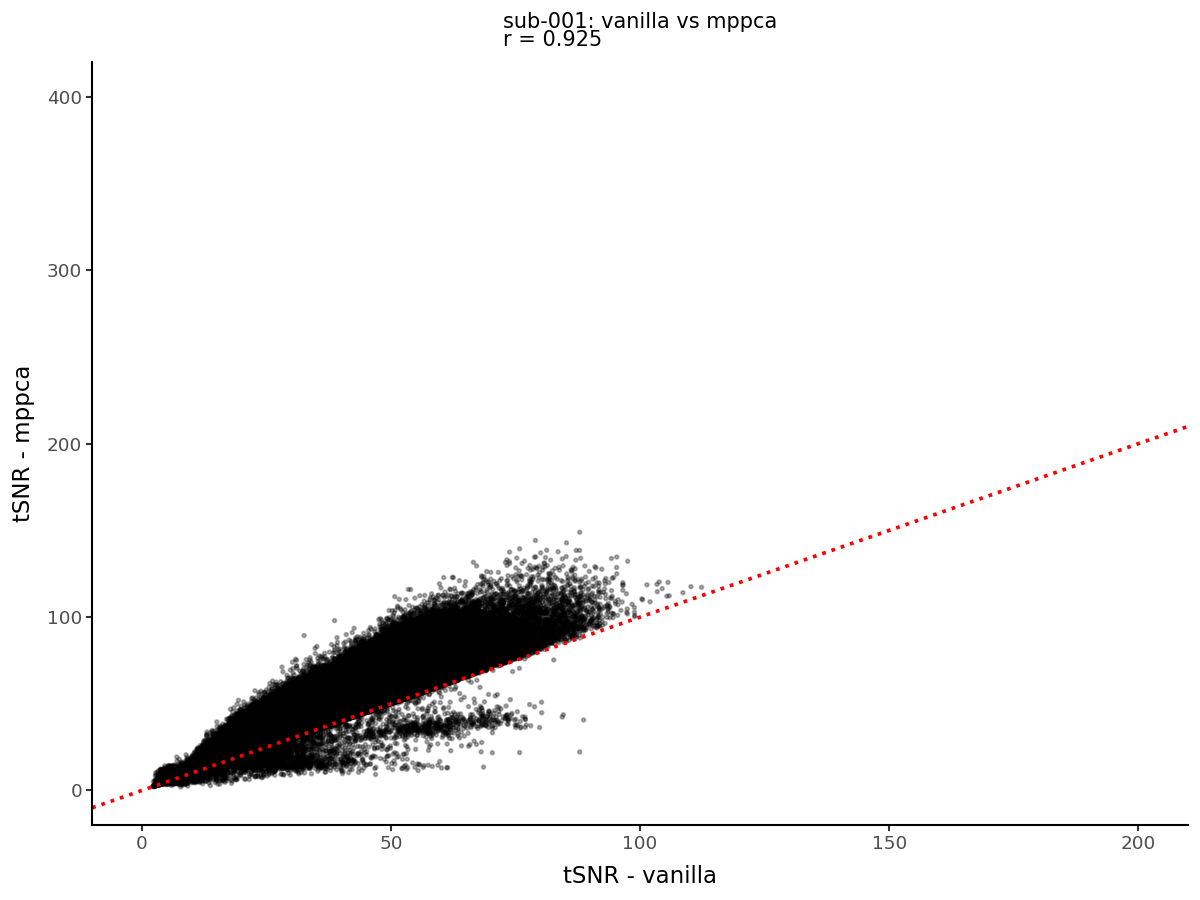
\includegraphics[width=2.5cm]{images/sub-001_vanilla_vs_mppca_tsnr_scatterHR.png}
       & 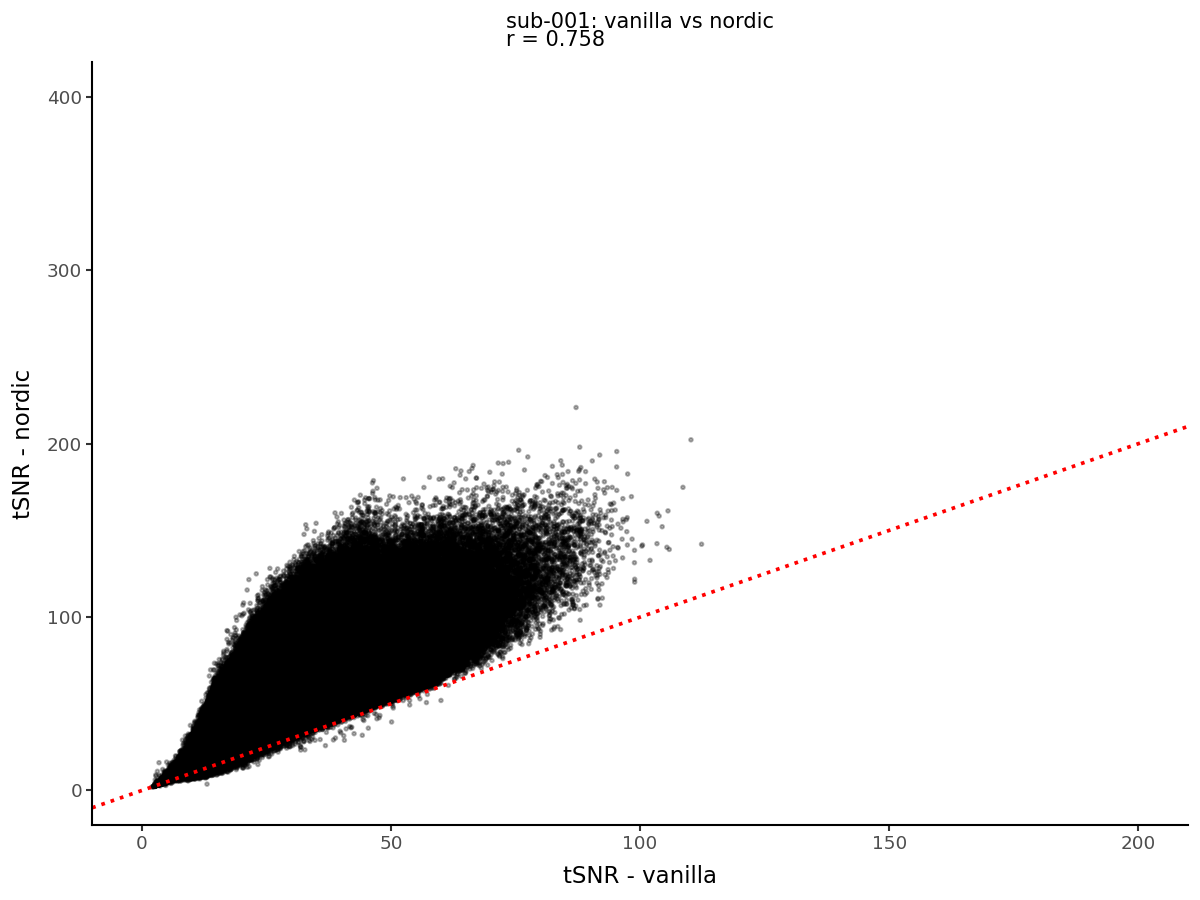
\includegraphics[width=2.5cm]{images/sub-001_vanilla_vs_nordic_tsnr_scatterHR.png}
       & 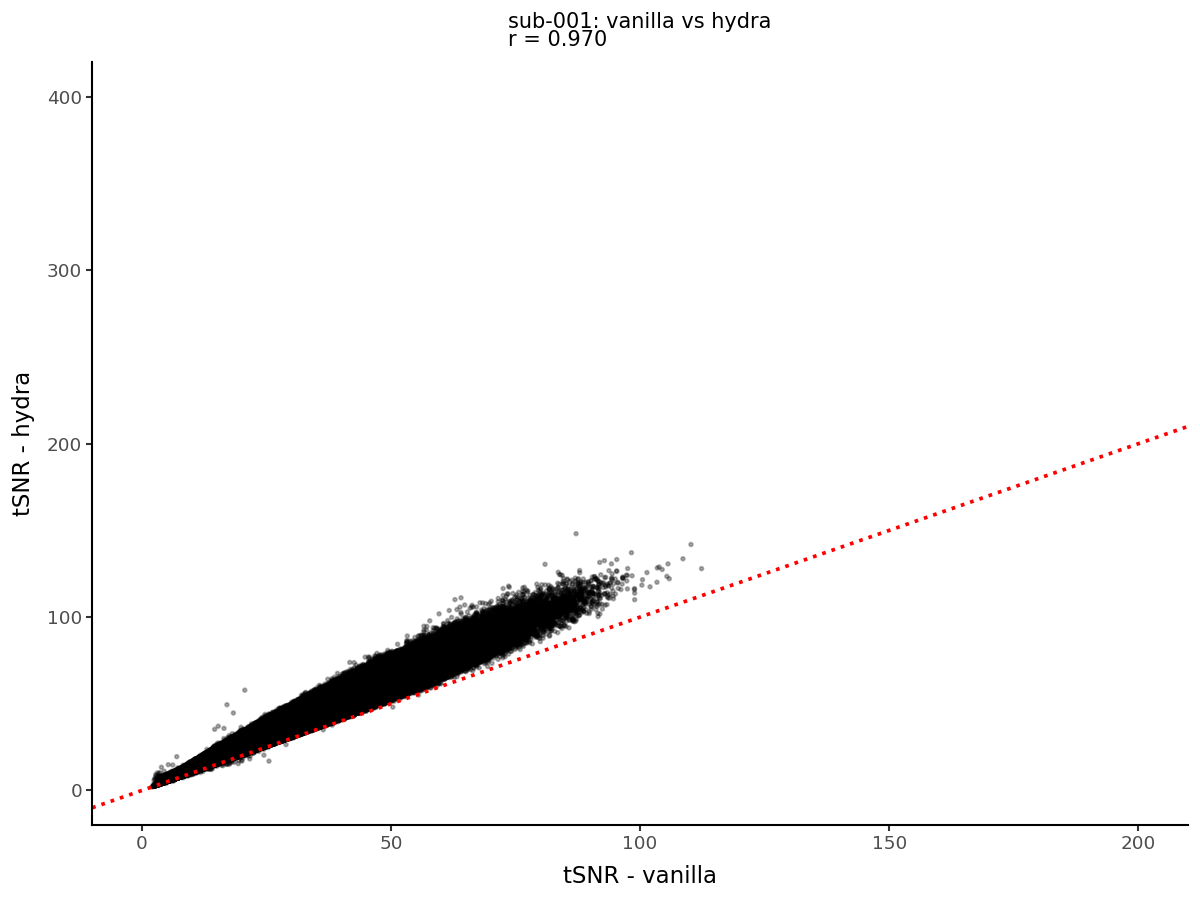
\includegraphics[width=2.5cm]{images/sub-001_vanilla_vs_hydra_tsnr_scatterHR.png}
       & 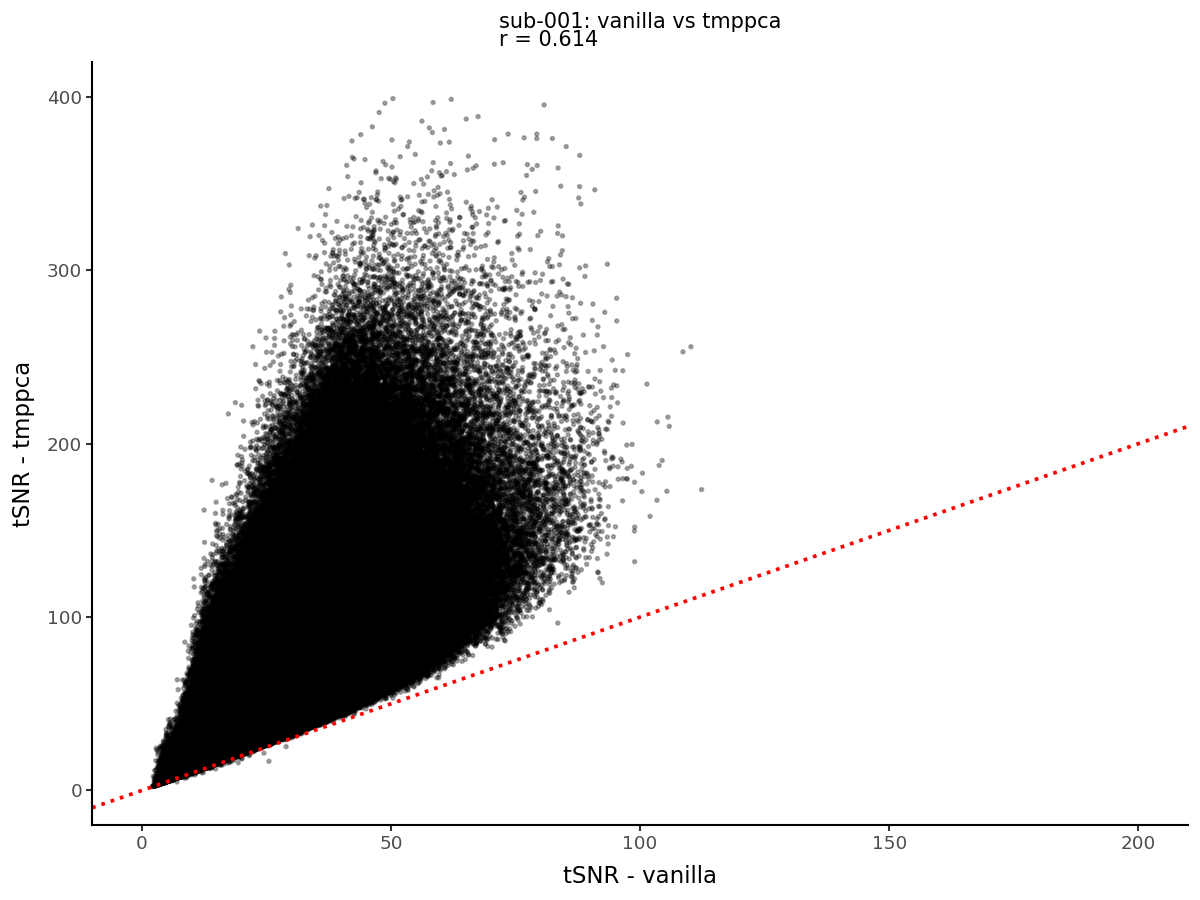
\includegraphics[width=2.5cm]{images/sub-001_vanilla_vs_tmppca_tsnr_scatterHR.png}
       \end{tabular}
    }
    \caption[tSNR scatterplots (1.5 mm isotropic)]{tSNR scatterplots (1.5 mm isotropic) comparing vanilla tSNR (x‑axis) versus tSNR after each denoising method (y‑axis). The identity line (red) represents no change.}
    \label{fig:scatterHR}
\end{figure}

The 1.5 mm dataset exhibits a lower SNR regime than its coarser counterparts. As shown in (Fig.~\ref{fig:tsnrHR}), a distinct pattern emerged compared to the high SNR datasets. Consistent with the 2 mm and 2.4 mm findings, TMPPCA yielded the highest tSNR overall. Nevertheless, in contrast to the observations in low resolution datasets, NORDIC produced higher tSNR values than MPPCA, which we conjecture arises from the forced spatial redundancy inherent to the method. TMPPCA-associated enhancement of tSNR was particularly evident in deeper regions of the brain, suggesting that TMPPCA may improve the feasibility of functional and structural investigations targeting these areas with high resolution. 

The $\Delta$tSNR maps further corroborated the superior performance of TMPPCA, as indicated by its larger spatial extent and magnitude of saturation. Here, NORDIC improved tSNR relative to both vanilla and MPPCA, whereas HYDRA did not yield a comparable enhancement. This discrepancy likely arises because the spatial redundancy due to the concatenation of the echoes might mix thermal noise variance with the signal of interest \citep{fernandesMPPCADenoisingFMRI2023a}, causing an underestimation of the $\lambda$ noise floor threshold \citep{manzanopatronDenoisingDiffusionMRI2024}. Similar to lower-resolution datasets, the $\Delta\%tSNR$ maps were predominantly positively saturated (i.e. $\Delta$tSNR values $\geqslant.5$), particularly for TMPPCA and NORDIC to a lower degree. Both approaches result in a notable increase in tSNR values across mostly the entire brain, except in regions with a strong vascular contribution, such as large vessels the sagittal sinus, where physiological noise dominates thermal noise. Conversely, MPPCA and HYDRA show lower increases in tSNR and $\Delta\%tSNR$ values, as also shown in (Fig.~\ref{fig:tsnrDistributionspc}).

The scatterplots in (Fig.~\ref{fig:scatterHR}) corroborated these observations. MPPCA yielded lower tSNR values than vanilla for a subset of voxels, while HYDRA produced only modest voxel-wise tSNR increases. In contrast, NORDIC consistently increased tSNR values, yet TMPPCA substantially outperformed all other methods on a per-voxel basis. 

\subsection{Relaxation times ($R_2^*$)}
%%%%%%-------
% -----------R 2
% -----------
%%%%%%-------
\begin{figure}[htbp]
\centering \colorbox{black}{
    \centering
    \begin{tabular}{>{\centering\arraybackslash}m{.7cm}>{\centering\arraybackslash}m{3cm}>{\centering\arraybackslash}m{3cm}>{\centering\arraybackslash}m{.7cm}}
    
       & \textcolor{white}{\textbf{$\overline{R_2^*}$}} & \textcolor{white}{\textbf{$\Delta\overline{R_2^*}$}}& \\
   \rotatebox[origin=l]{90}{\textcolor{white}{VANILLA}}
  &    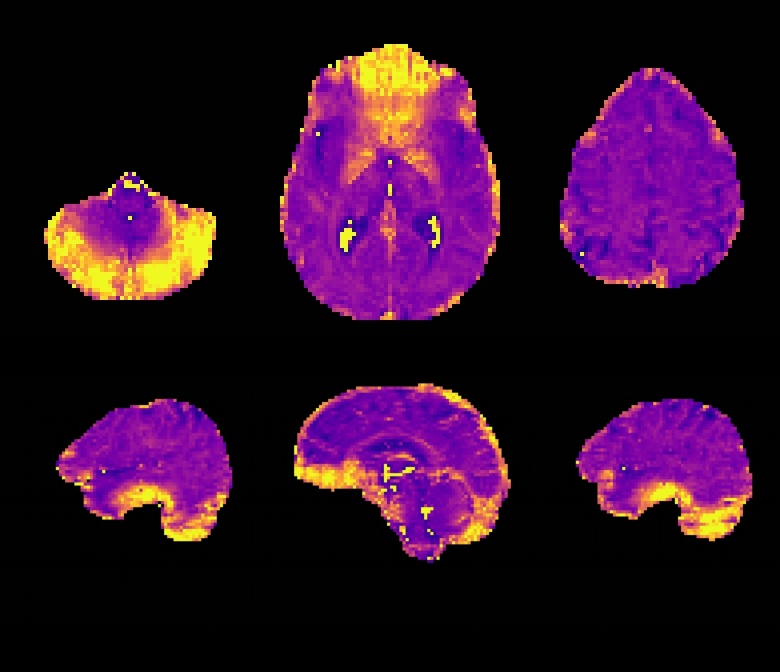
\includegraphics[width=3cm]{images/sub-001_ses-1_task-HABLA1200_R2mean_part-mag_bold_vanilla_all.jpg} & & \textcolor{white}{$\overline{R_2^*}$} 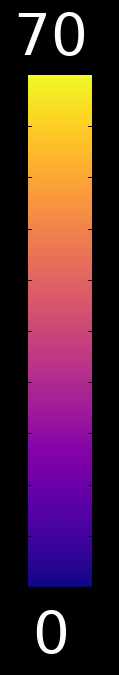
\includegraphics[width=.5cm]{images/Plasmar2.png}\\
     \rotatebox[origin=l]{90}{\textcolor{white}{MPPCA}}
  &    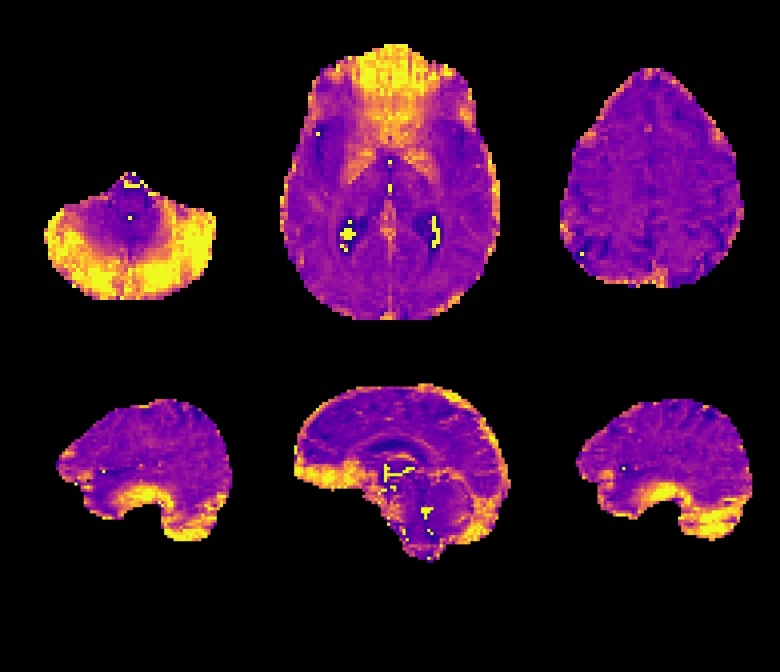
\includegraphics[width=3cm]{images/sub-001_ses-1_task-HABLA1200_R2mean_part-mag_bold_mppca_all} &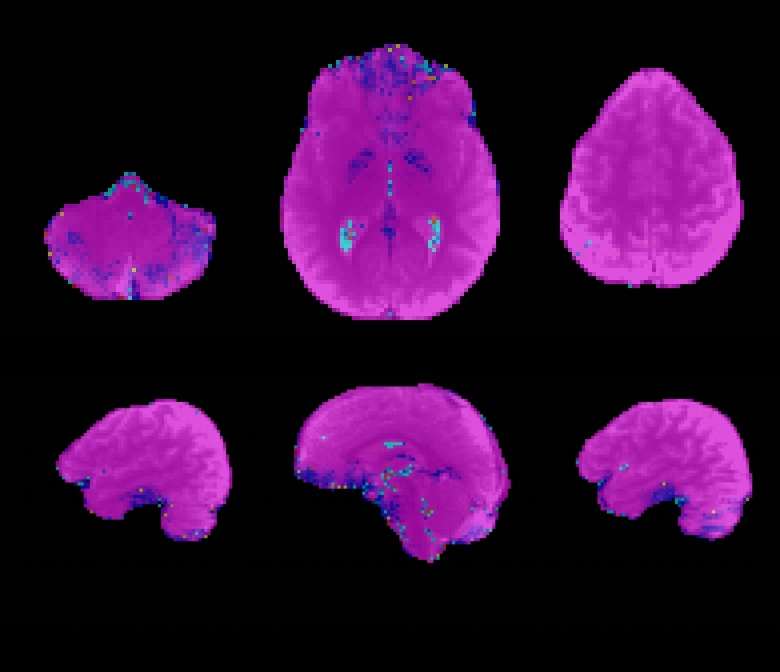
\includegraphics[width=3cm]{images/sub-001_ses-1_task-HABLA1200_R2meanSPC_part-mag_bold_mppca_all} &\\
       \rotatebox[origin=l]{90}{\textcolor{white}{NORDIC}}
  &    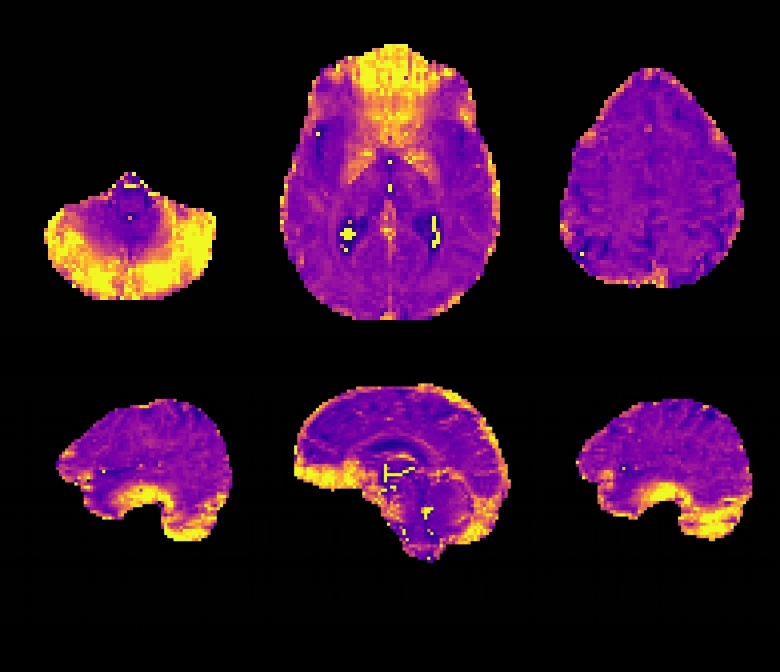
\includegraphics[width=3cm]{images/sub-001_ses-1_task-HABLA1200_R2mean_part-mag_bold_nordic_all.jpg} &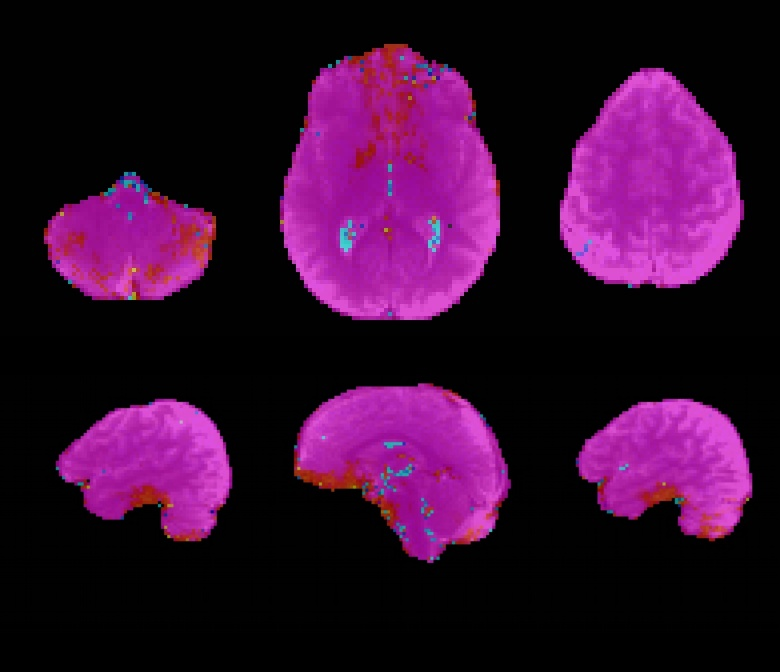
\includegraphics[width=3cm]{images/sub-001_ses-1_task-HABLA1200_R2meanSPC_part-mag_bold_nordic_all} &\\
       \rotatebox[origin=l]{90}{\textcolor{white}{HYDRA}}
  &    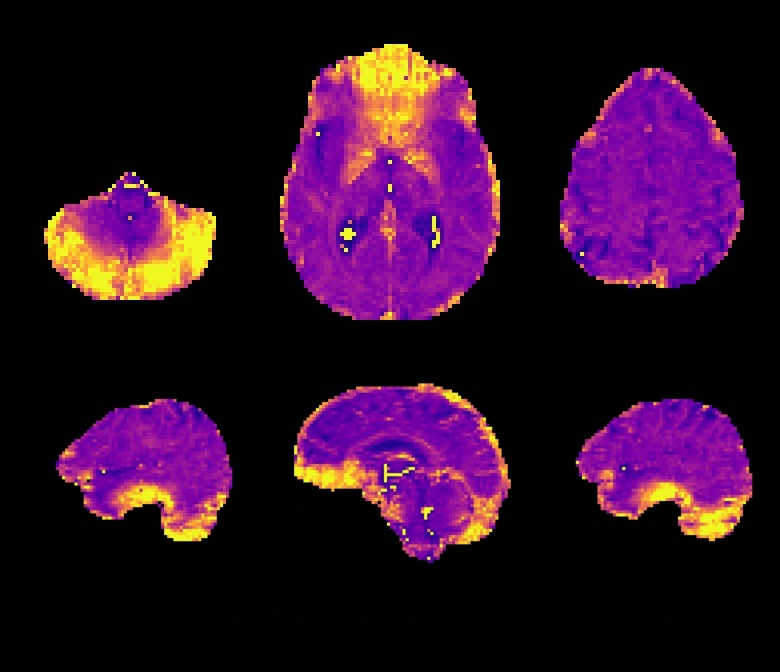
\includegraphics[width=3cm]{images/sub-001_ses-1_task-HABLA1200_R2mean_part-mag_bold_hydra_all.jpg} &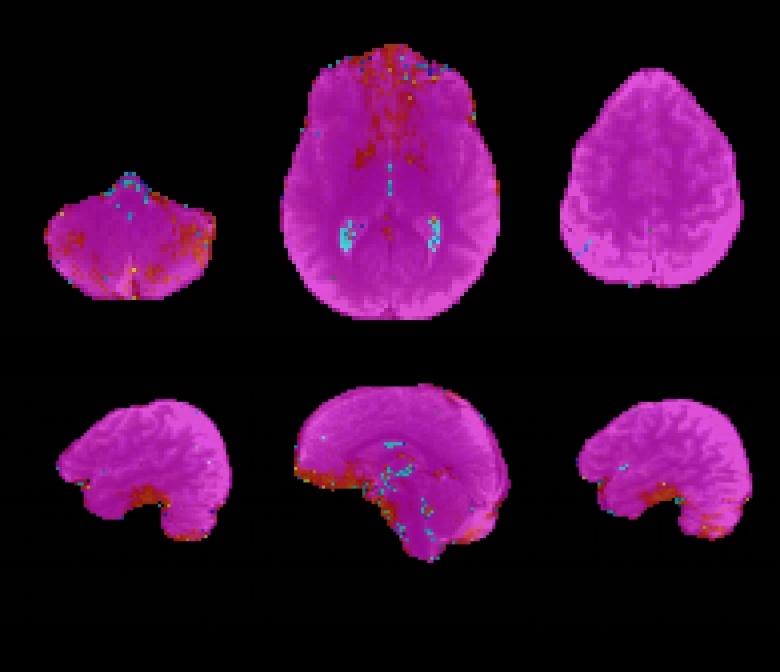
\includegraphics[width=3cm]{images/sub-001_ses-1_task-HABLA1200_R2meanSPC_part-mag_bold_hydra_all} &\\
       \rotatebox[origin=l]{90}{\textcolor{white}{TMPPCA}}
  &    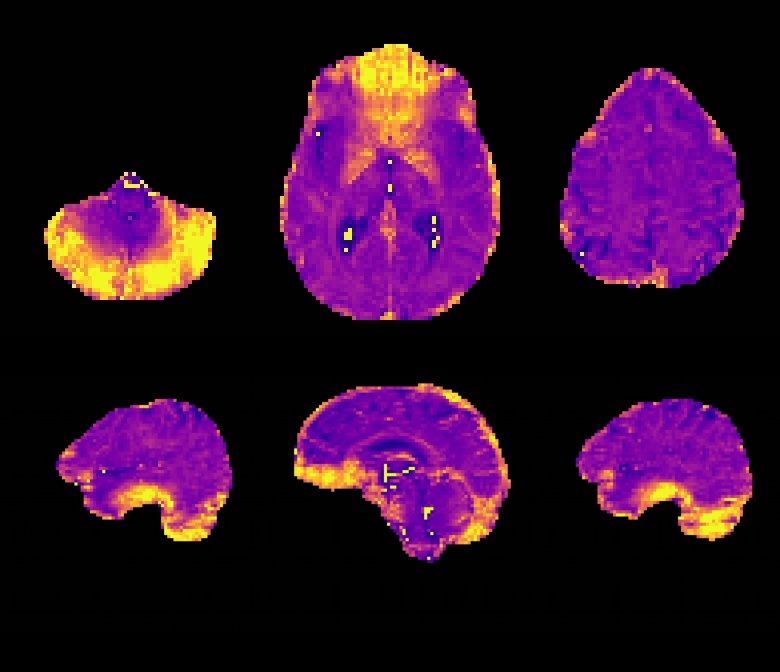
\includegraphics[width=3cm]{images/sub-001_ses-1_task-HABLA1200_R2mean_part-mag_bold_tmppca_all.jpg} &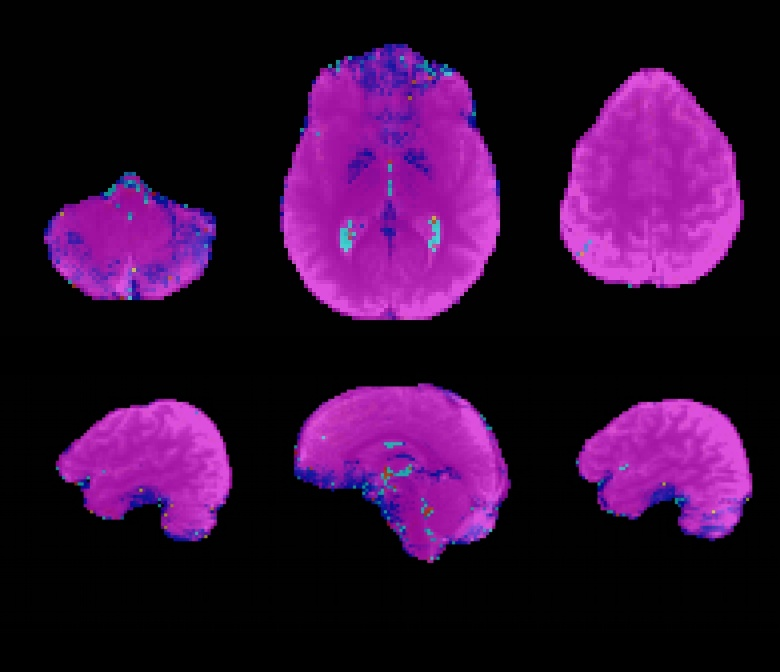
\includegraphics[width=3cm]{images/sub-001_ses-1_task-HABLA1200_R2meanSPC_part-mag_bold_tmppca_all} &\textcolor{white}{$\Delta \overline{R_2^*}$} 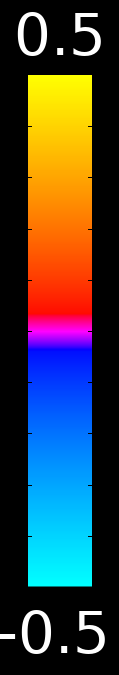
\includegraphics[width=.5cm]{images/SPC.png}\\
    \end{tabular}
    }
        \caption[$\overline{R_2^*}$  maps, low resolution (2.4 mm isotropic)]{Left: $\overline{R_2^*}$ maps (2.4 mm, saturation at 70 s$^{-1}$). Right: $\Delta\overline{R_2^*}$ (change relative to vanilla).}
    \label{fig:R21200}
\end{figure}

\begin{figure}[htbp]
\centering \colorbox{black}{
    \centering
    \begin{tabular}{>{\centering\arraybackslash}m{.7cm}>{\centering\arraybackslash}m{3cm}>{\centering\arraybackslash}m{3cm}>{\centering\arraybackslash}m{.7cm}}
    
       & \textcolor{white}{\textbf{$\overline{R_2^*}$}} & \textcolor{white}{\textbf{$\Delta \overline{R_2^*}$}}& \\
   \rotatebox[origin=l]{90}{\textcolor{white}{VANILLA}}
  &    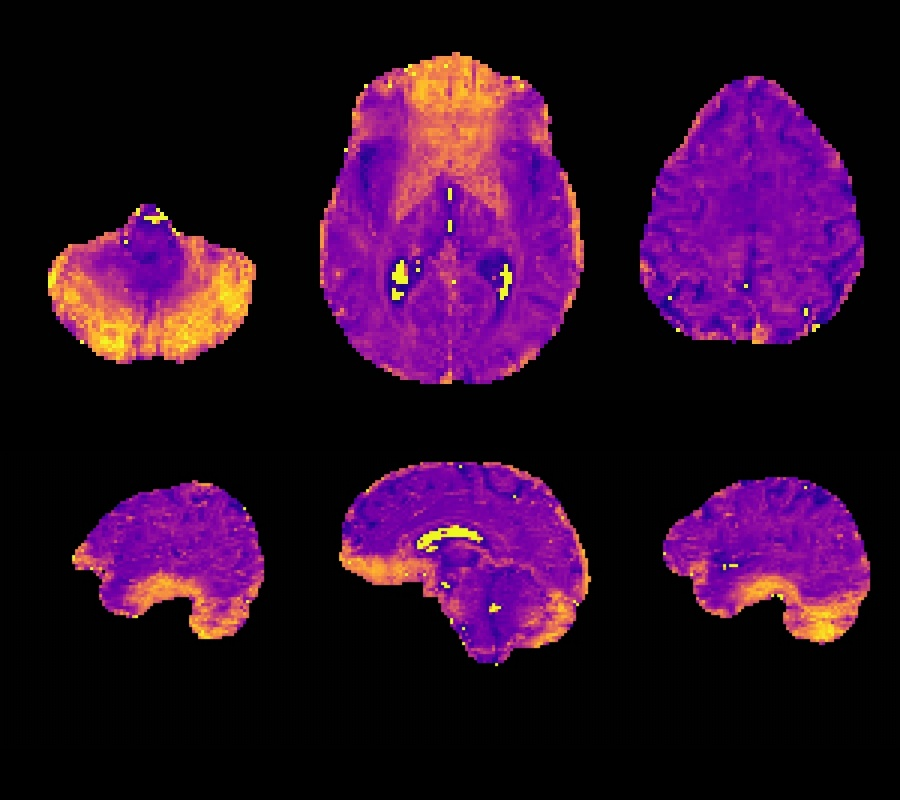
\includegraphics[width=3cm]{images/sub-001_ses-1_task-HABLA1700_R2mean_part-mag_bold_vanilla_all.jpg} & & \textcolor{white}{$R_2^*$} 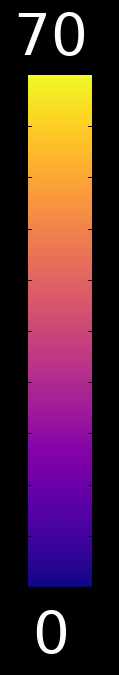
\includegraphics[width=.5cm]{images/Plasmar2.png}\\
     \rotatebox[origin=l]{90}{\textcolor{white}{MPPCA}}
  &    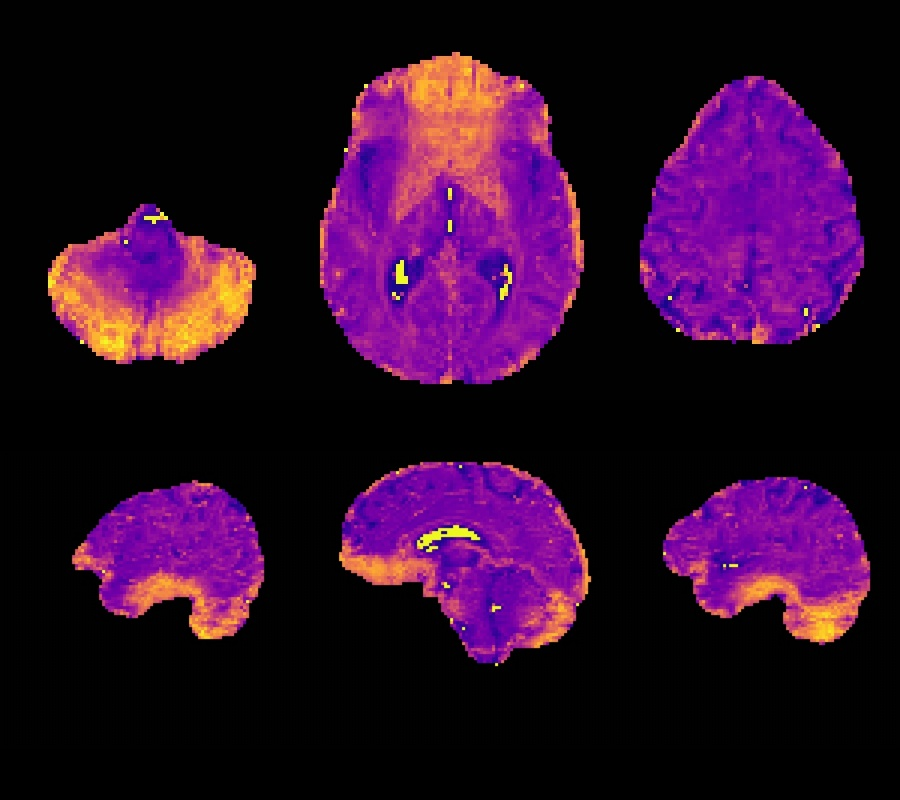
\includegraphics[width=3cm]{images/sub-001_ses-1_task-HABLA1700_R2mean_part-mag_bold_mppca_all} &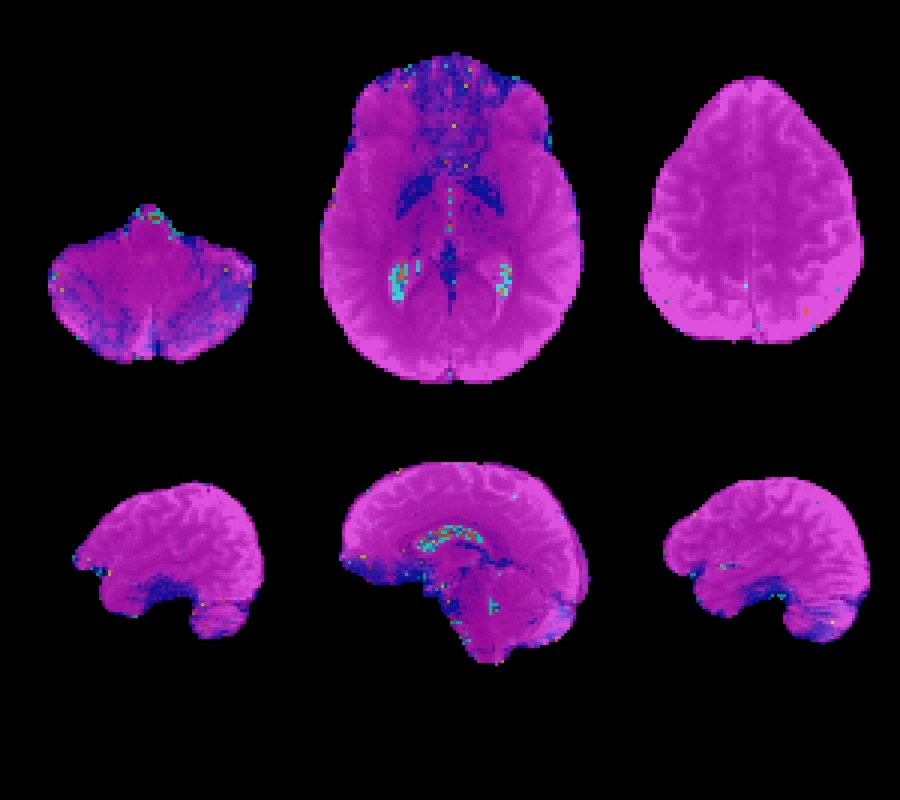
\includegraphics[width=3cm]{images/sub-001_ses-1_task-HABLA1700_R2meanSPC_part-mag_bold_mppca_all} &\\
       \rotatebox[origin=l]{90}{\textcolor{white}{NORDIC}}
  &    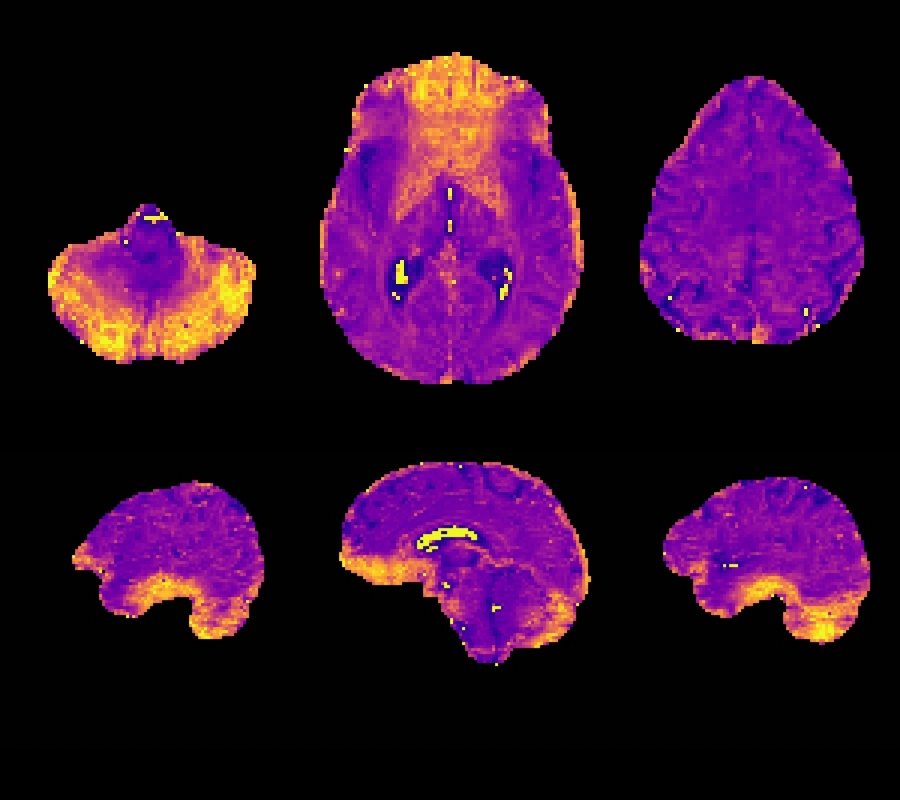
\includegraphics[width=3cm]{images/sub-001_ses-1_task-HABLA1700_R2mean_part-mag_bold_nordic_all.jpg} &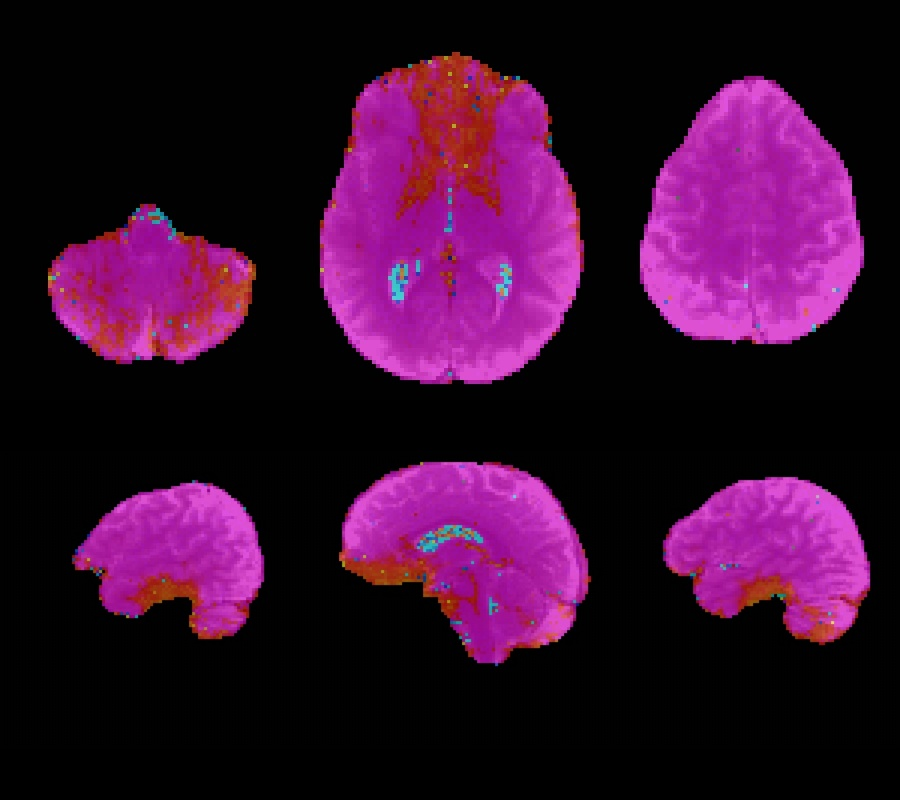
\includegraphics[width=3cm]{images/sub-001_ses-1_task-HABLA1700_R2meanSPC_part-mag_bold_nordic_all} &\\
       \rotatebox[origin=l]{90}{\textcolor{white}{HYDRA}}
  &    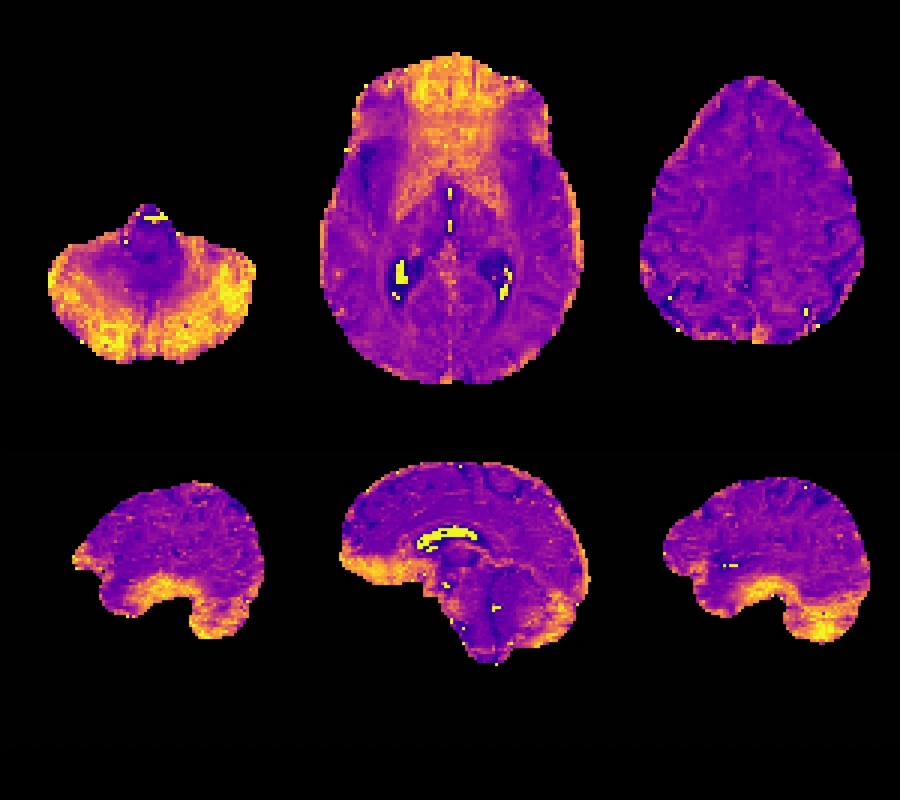
\includegraphics[width=3cm]{images/sub-001_ses-1_task-HABLA1700_R2mean_part-mag_bold_hydra_all.jpg} &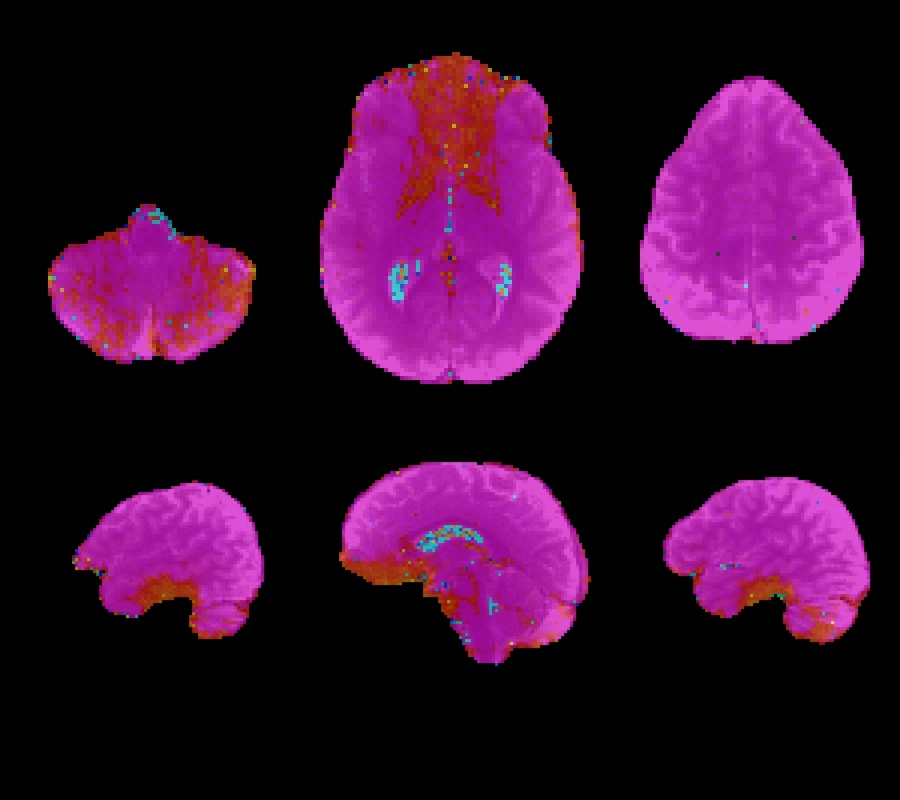
\includegraphics[width=3cm]{images/sub-001_ses-1_task-HABLA1700_R2meanSPC_part-mag_bold_hydra_all} &\\
       \rotatebox[origin=l]{90}{\textcolor{white}{TMPPCA}}
  &    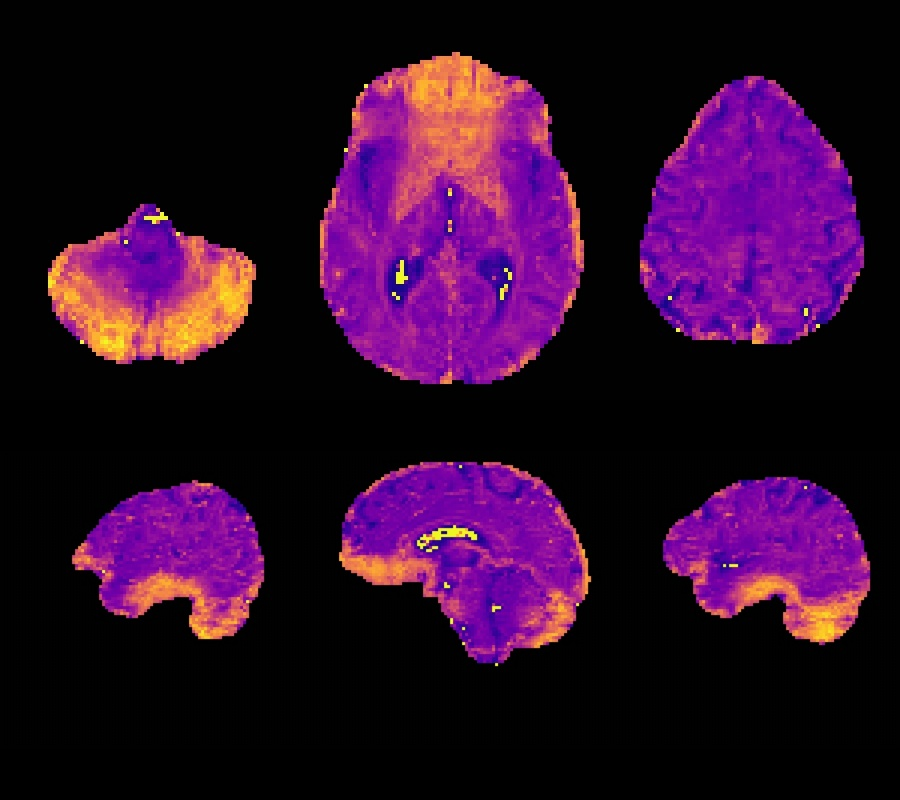
\includegraphics[width=3cm]{images/sub-001_ses-1_task-HABLA1700_R2mean_part-mag_bold_tmppca_all.jpg} &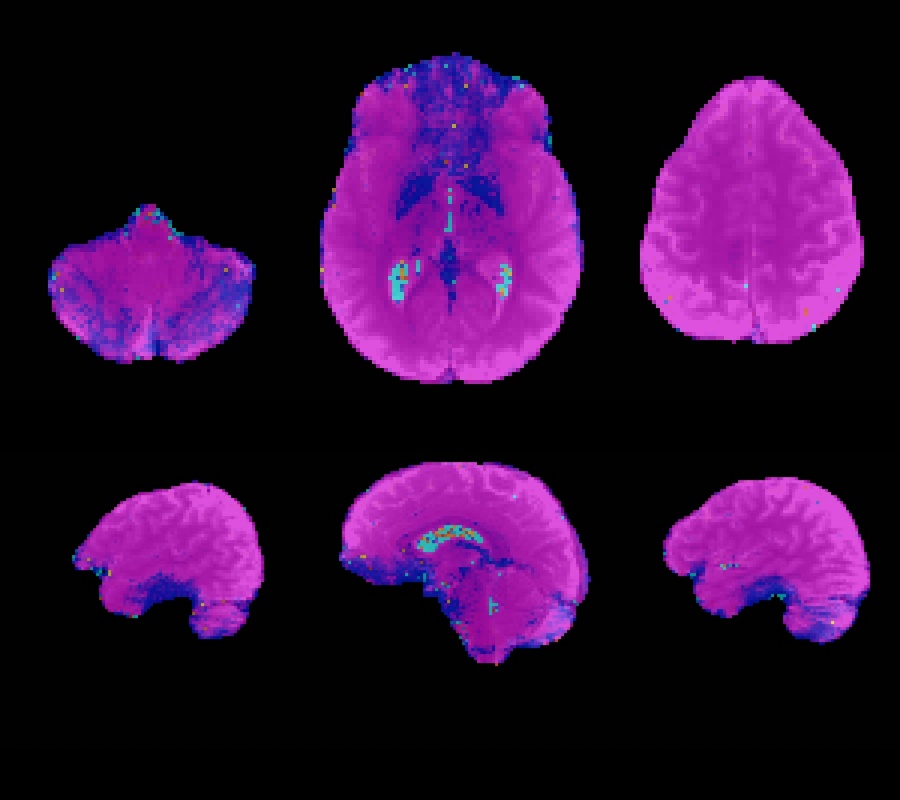
\includegraphics[width=3cm]{images/sub-001_ses-1_task-HABLA1700_R2meanSPC_part-mag_bold_tmppca_all} &\textcolor{white}{$\Delta \overline{R_2^*}$} 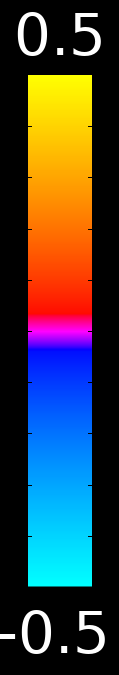
\includegraphics[width=.5cm]{images/SPC.png}\\
    \end{tabular}
    }
    \caption[$\overline{R_2^*}$ maps, low resolution (2 mm isotropic)]{Left: $\overline{R_2^*}$ maps (2 mm, saturation at 70 s$^{-1}$). Right: $\Delta\overline{R_2^*}$ (change relative to vanilla).}
    \label{fig:R21700}
\end{figure}

\begin{figure}[htbp]
\centering \colorbox{black}{
    \centering
    \begin{tabular}{>{\centering\arraybackslash}m{.7cm}>{\centering\arraybackslash}m{3cm}>{\centering\arraybackslash}m{3cm}>{\centering\arraybackslash}m{.7cm}}
    
       & \textcolor{white}{\textbf{$\overline{R_2^*}$}} & \textcolor{white}{\textbf{$\Delta  \overline{R_2^*}$}}& \\
   \rotatebox[origin=l]{90}{\textcolor{white}{VANILLA}}
  &    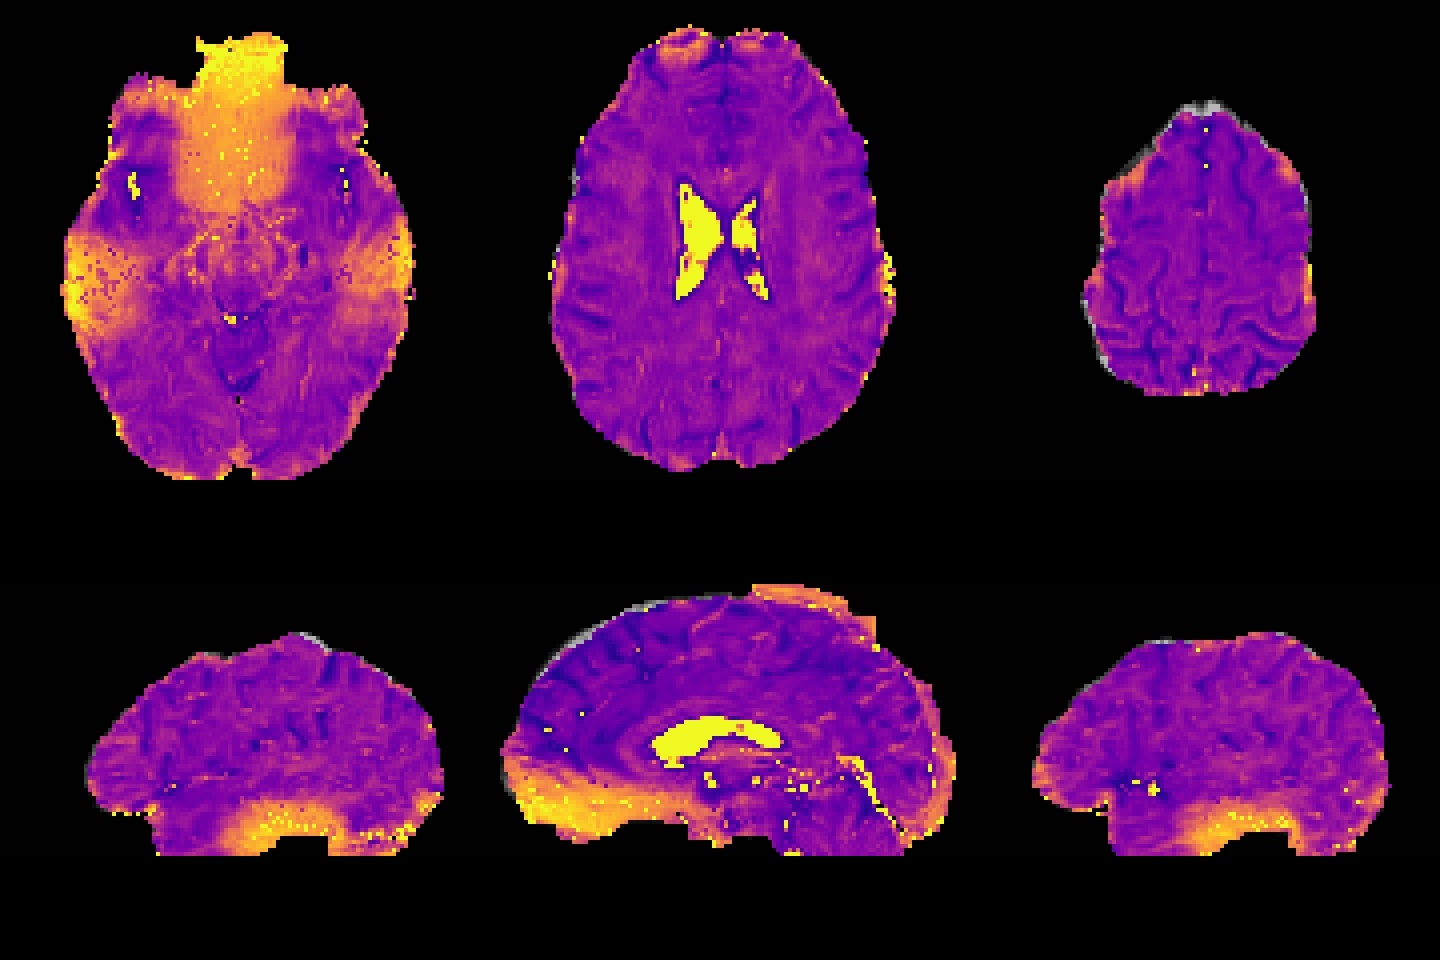
\includegraphics[width=3cm]{images/sub-001_ses-1_task-REST_run-1_R2mean_part-mag_bold_vanilla_all.jpg} & & \textcolor{white}{$\overline{R_2^*}$} 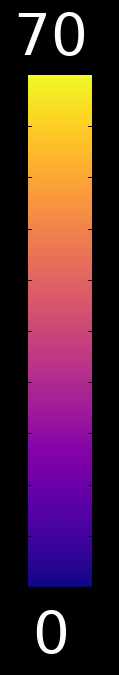
\includegraphics[width=.5cm]{images/Plasmar2.png}\\
     \rotatebox[origin=l]{90}{\textcolor{white}{MPPCA}}
  &    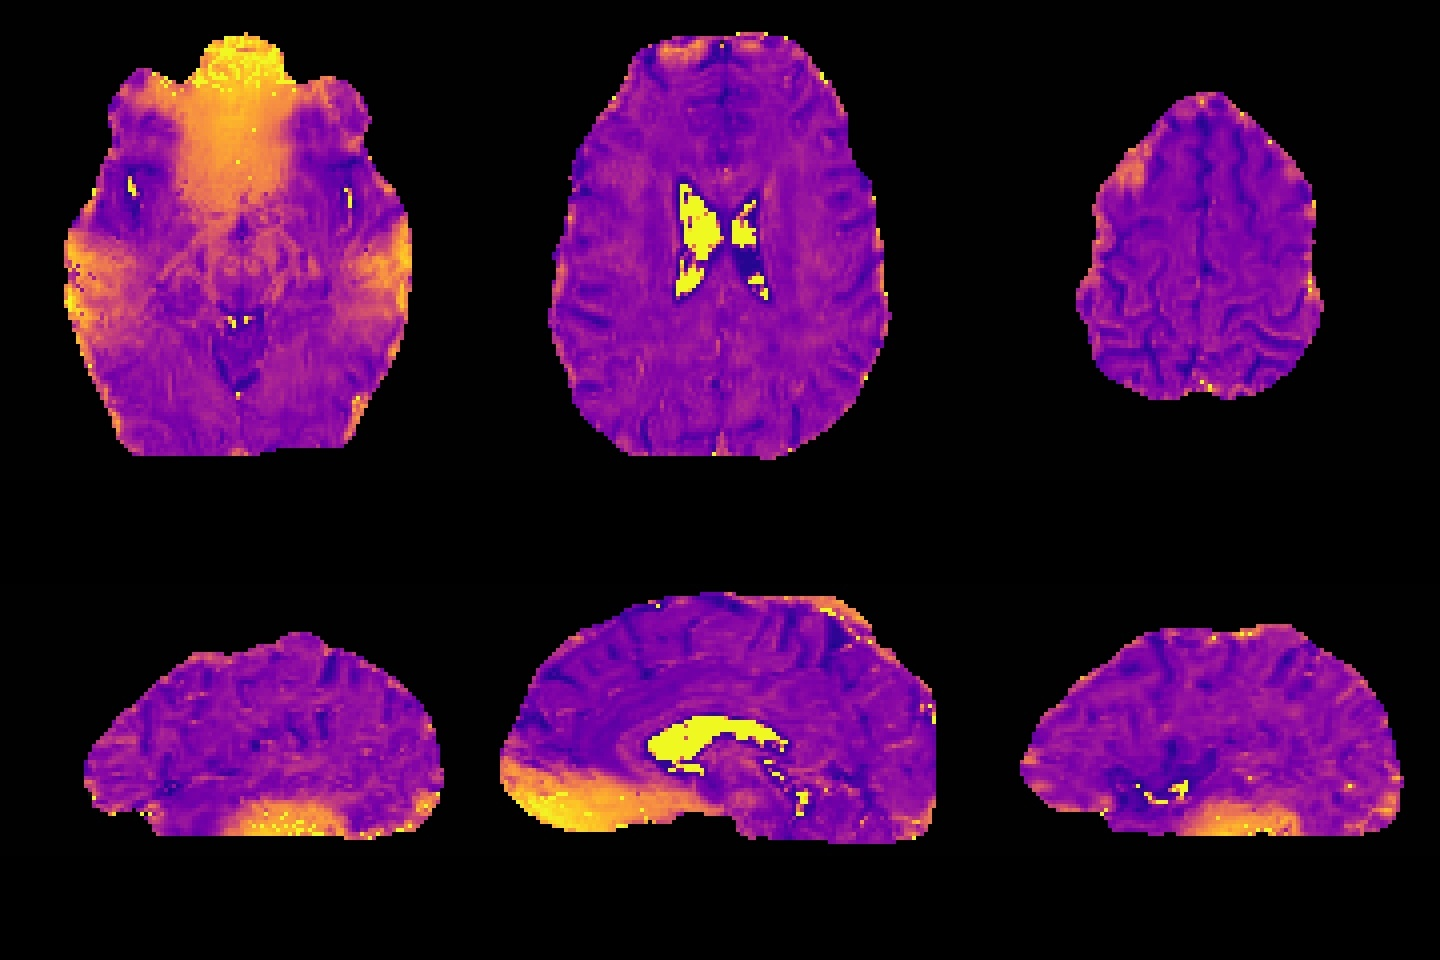
\includegraphics[width=3cm]{images/sub-001_ses-1_task-REST_run-1_R2mean_part-mag_bold_mppca_all} &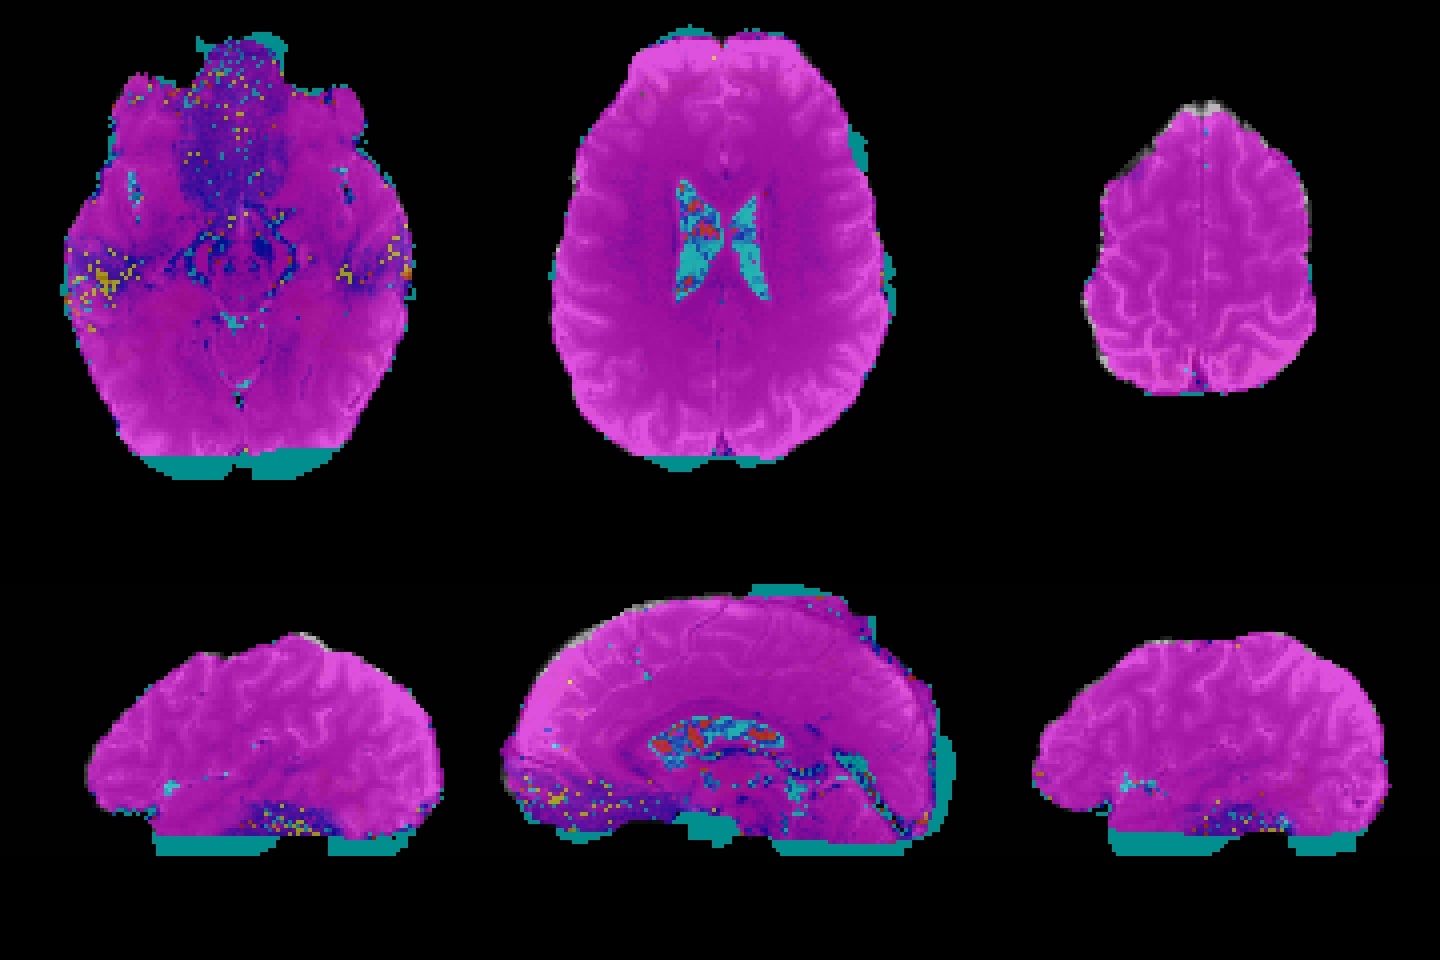
\includegraphics[width=3cm]{images/sub-001_ses-1_task-REST_run-1_R2meanSPC_part-mag_bold_mppca_all} &\\
       \rotatebox[origin=l]{90}{\textcolor{white}{NORDIC}}
  &    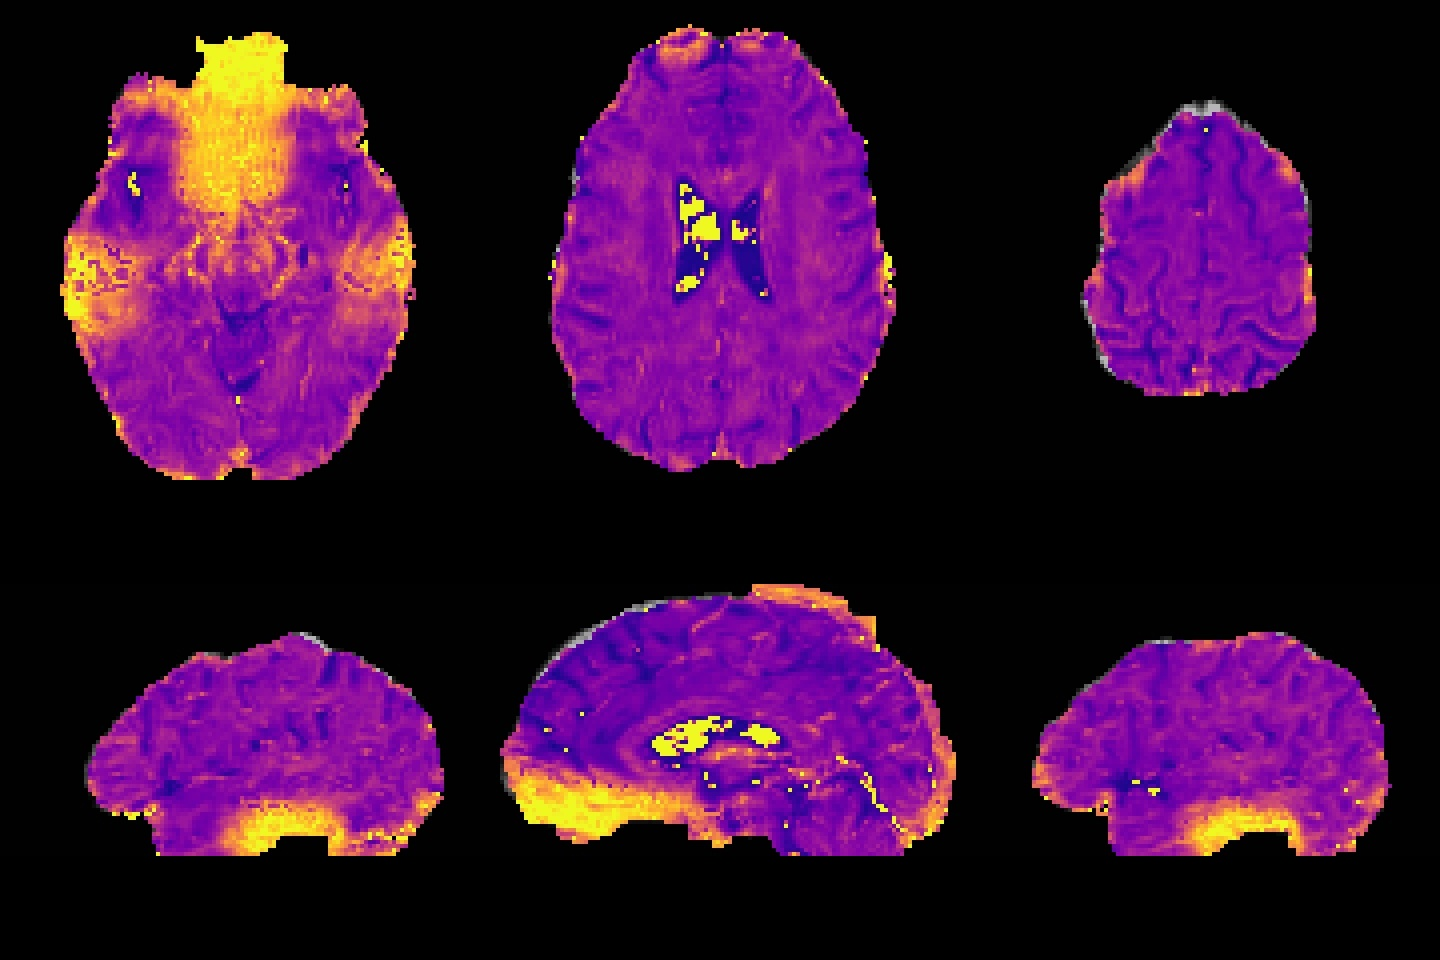
\includegraphics[width=3cm]{images/sub-001_ses-1_task-REST_run-1_R2mean_part-mag_bold_nordic_all.jpg} &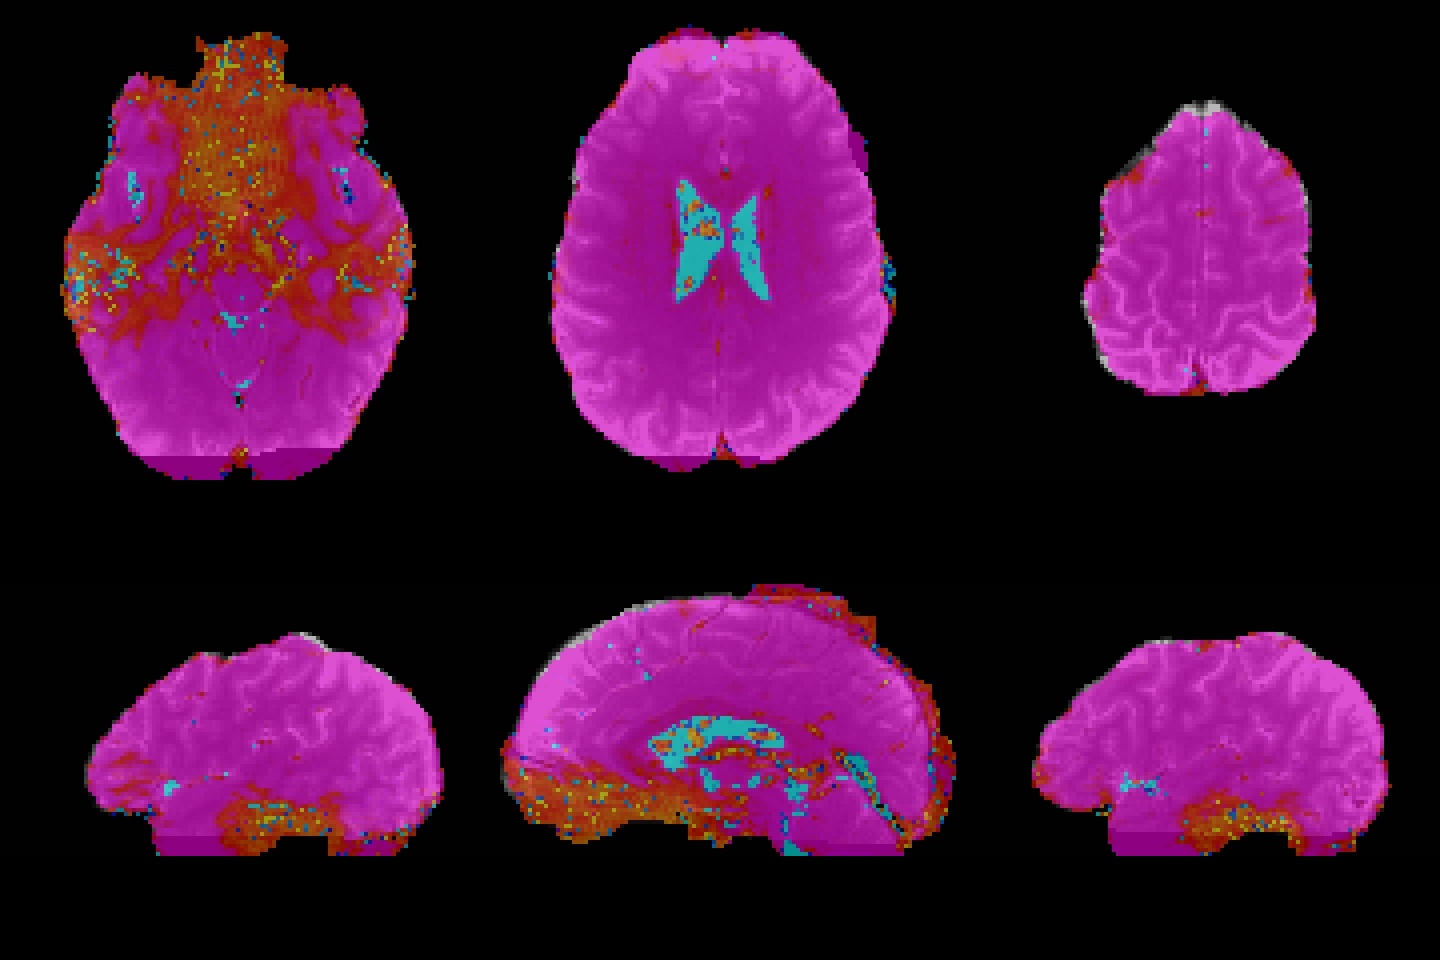
\includegraphics[width=3cm]{images/sub-001_ses-1_task-REST_run-1_R2meanSPC_part-mag_bold_nordic_all} &\\
       \rotatebox[origin=l]{90}{\textcolor{white}{HYDRA}}
  &    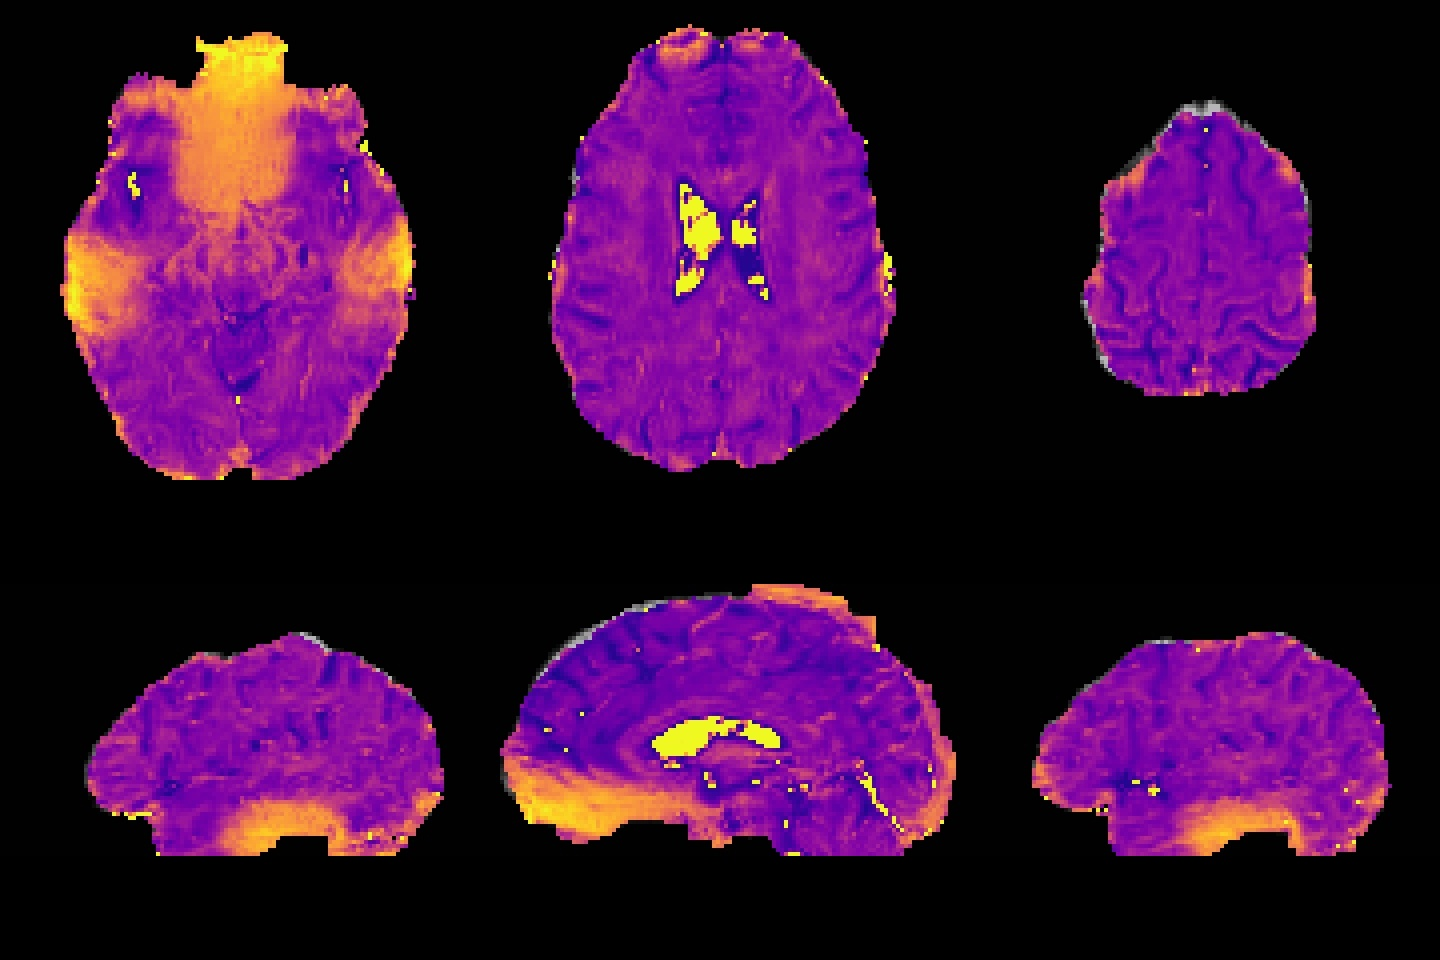
\includegraphics[width=3cm]{images/sub-001_ses-1_task-REST_run-1_R2mean_part-mag_bold_hydra_all.jpg} &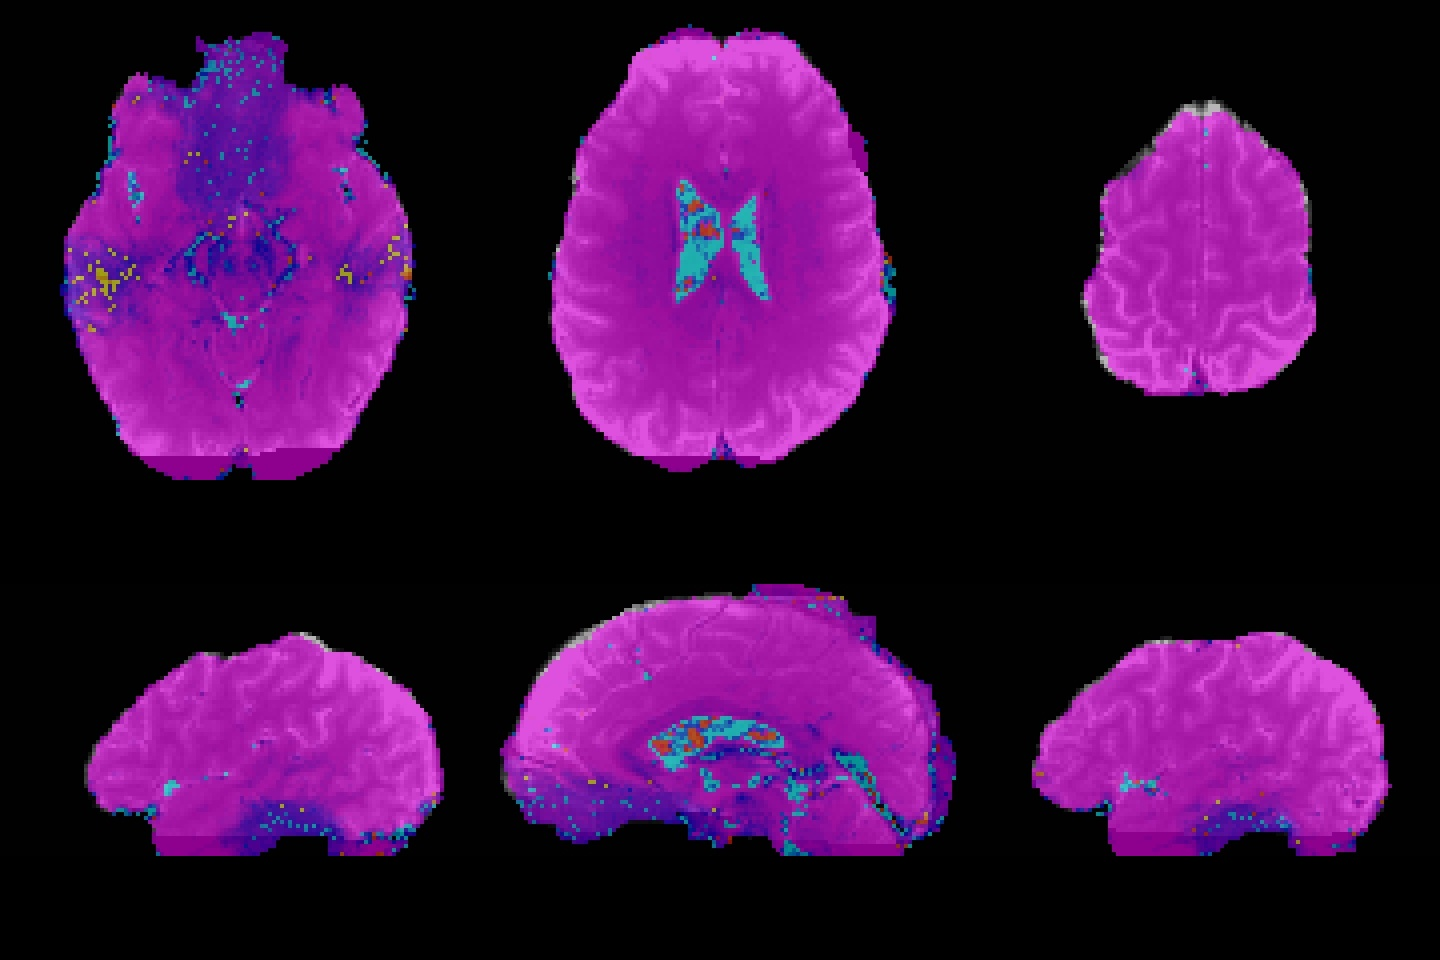
\includegraphics[width=3cm]{images/sub-001_ses-1_task-REST_run-1_R2meanSPC_part-mag_bold_hydra_all} &\\
       \rotatebox[origin=l]{90}{\textcolor{white}{TMPPCA}}
  &    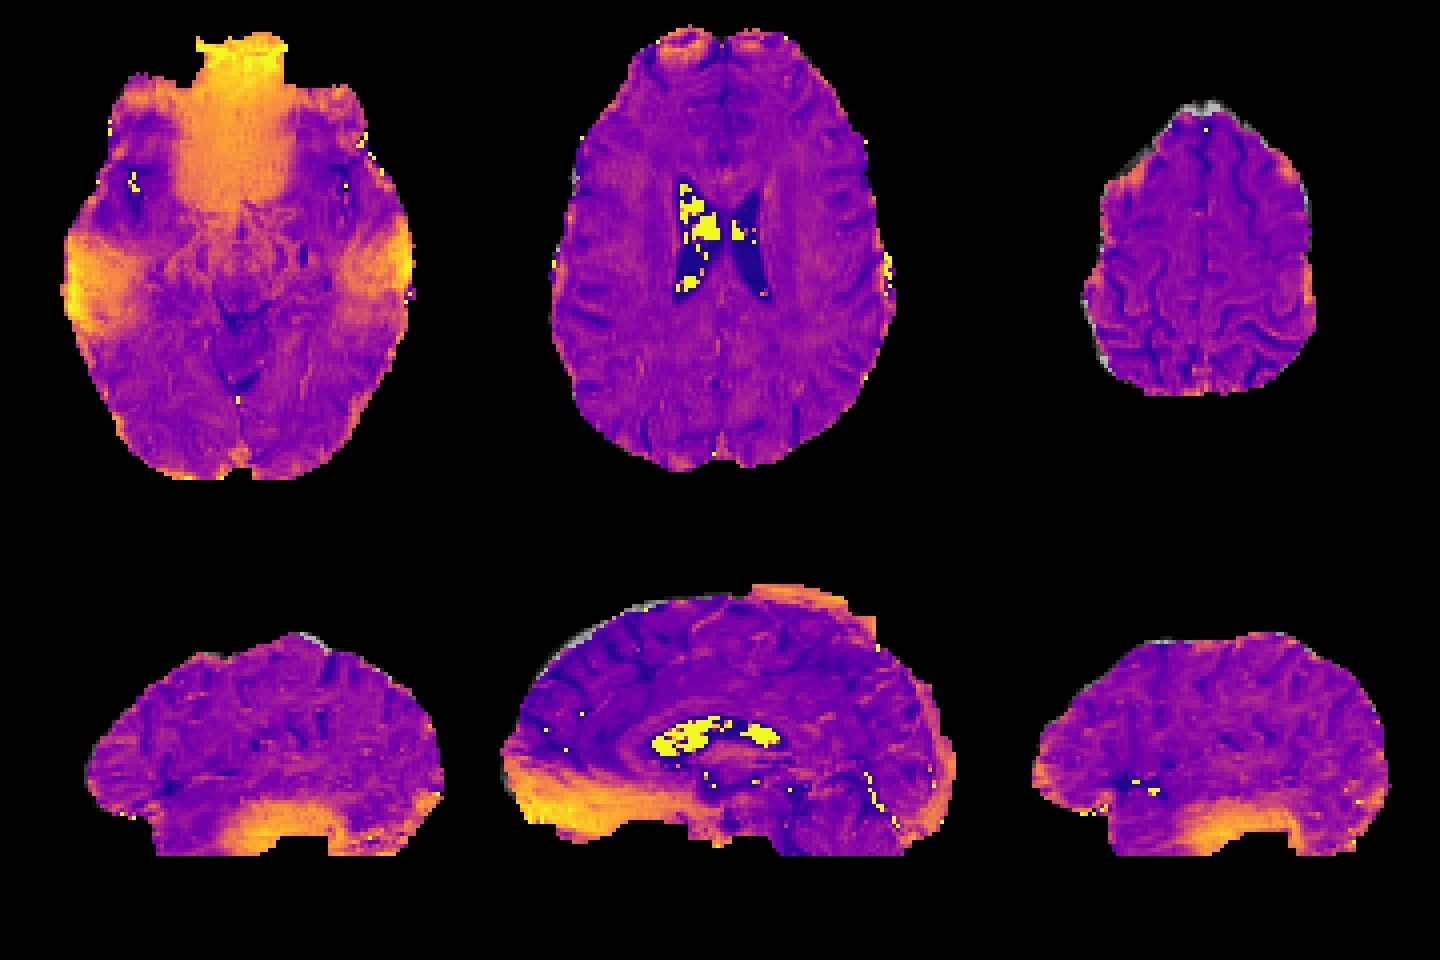
\includegraphics[width=3cm]{images/sub-001_ses-1_task-REST_run-1_R2mean_part-mag_bold_tmppca_all.jpg} &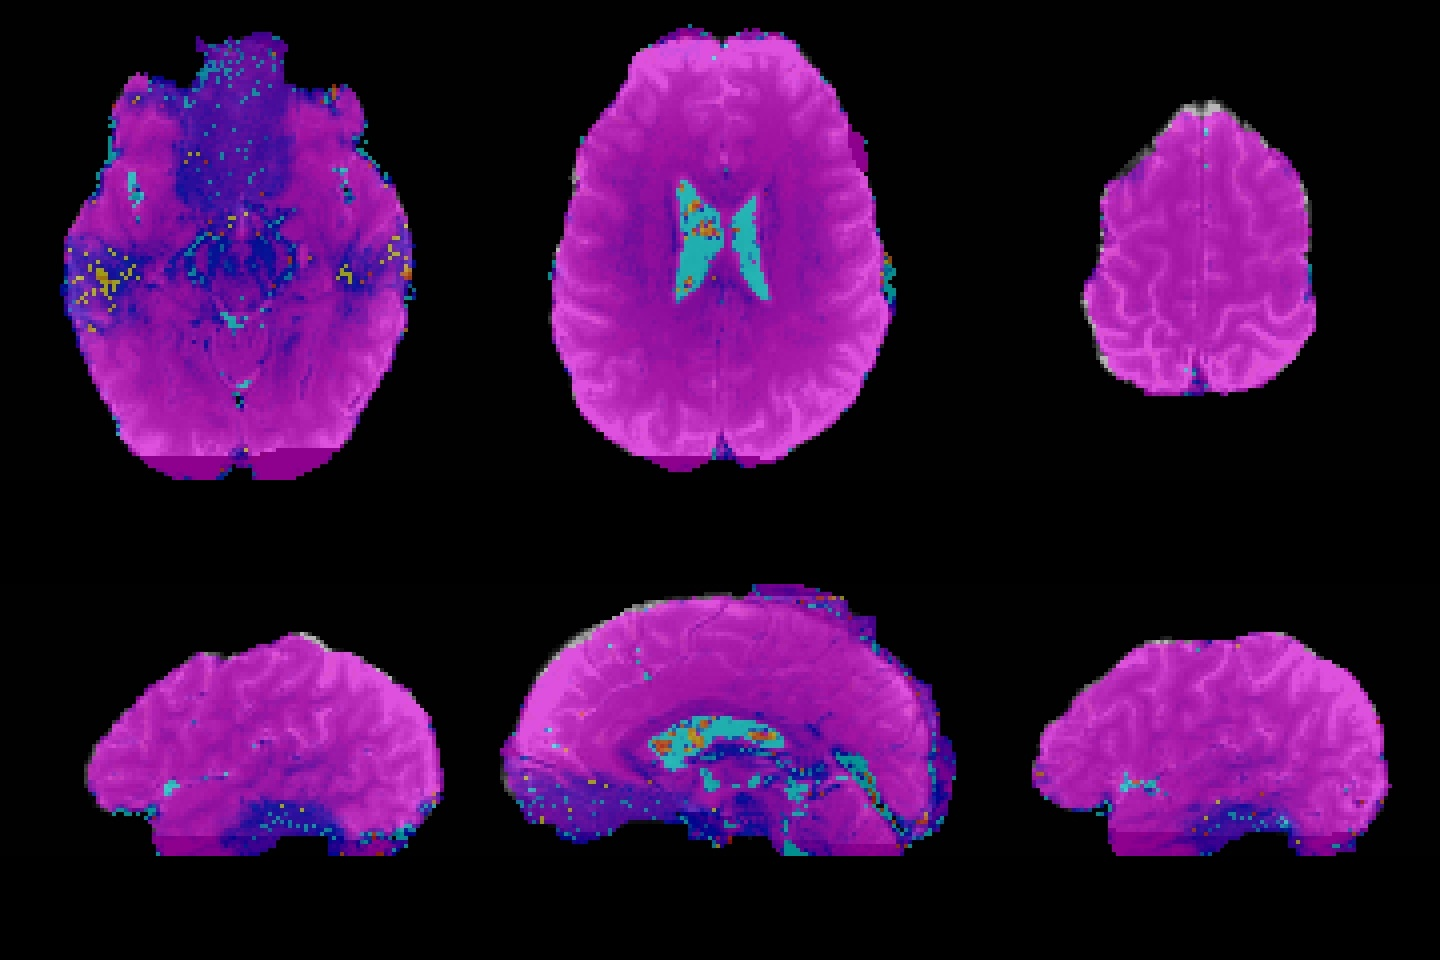
\includegraphics[width=3cm]{images/sub-001_ses-1_task-REST_run-1_R2meanSPC_part-mag_bold_tmppca_all} &\textcolor{white}{$\Delta \overline{R_2^*}$} 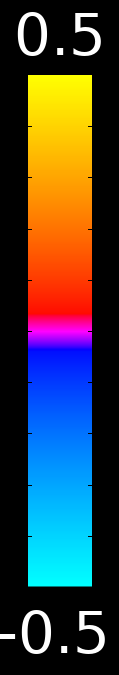
\includegraphics[width=.5cm]{images/SPC.png}\\
    \end{tabular}
    }
    \caption[$\overline{R_2^*}$  maps, high resolution (1.5 mm)]{Left: $\overline{R_2^*}$ maps (1.5 mm, saturation at 70 s$^{-1}$). Right: $\Delta\overline{R_2^*}$ (\% change relative to vanilla).}
    \label{fig:R2HR}
\end{figure}
%-- boxplots
%-- R2
\begin{figure}[htbp]
\centering \colorbox{white}{
    \centering
    \begin{tabular}{>{\centering\arraybackslash}m{.7cm}>{\centering\arraybackslash}m{10cm}}
       & \textcolor{black}{\textbf{$\overline{R_2^*}$ Distribution Across methods}} \\
    \rotatebox[origin=l]{90}{\textcolor{black}{2.4 mm}} &    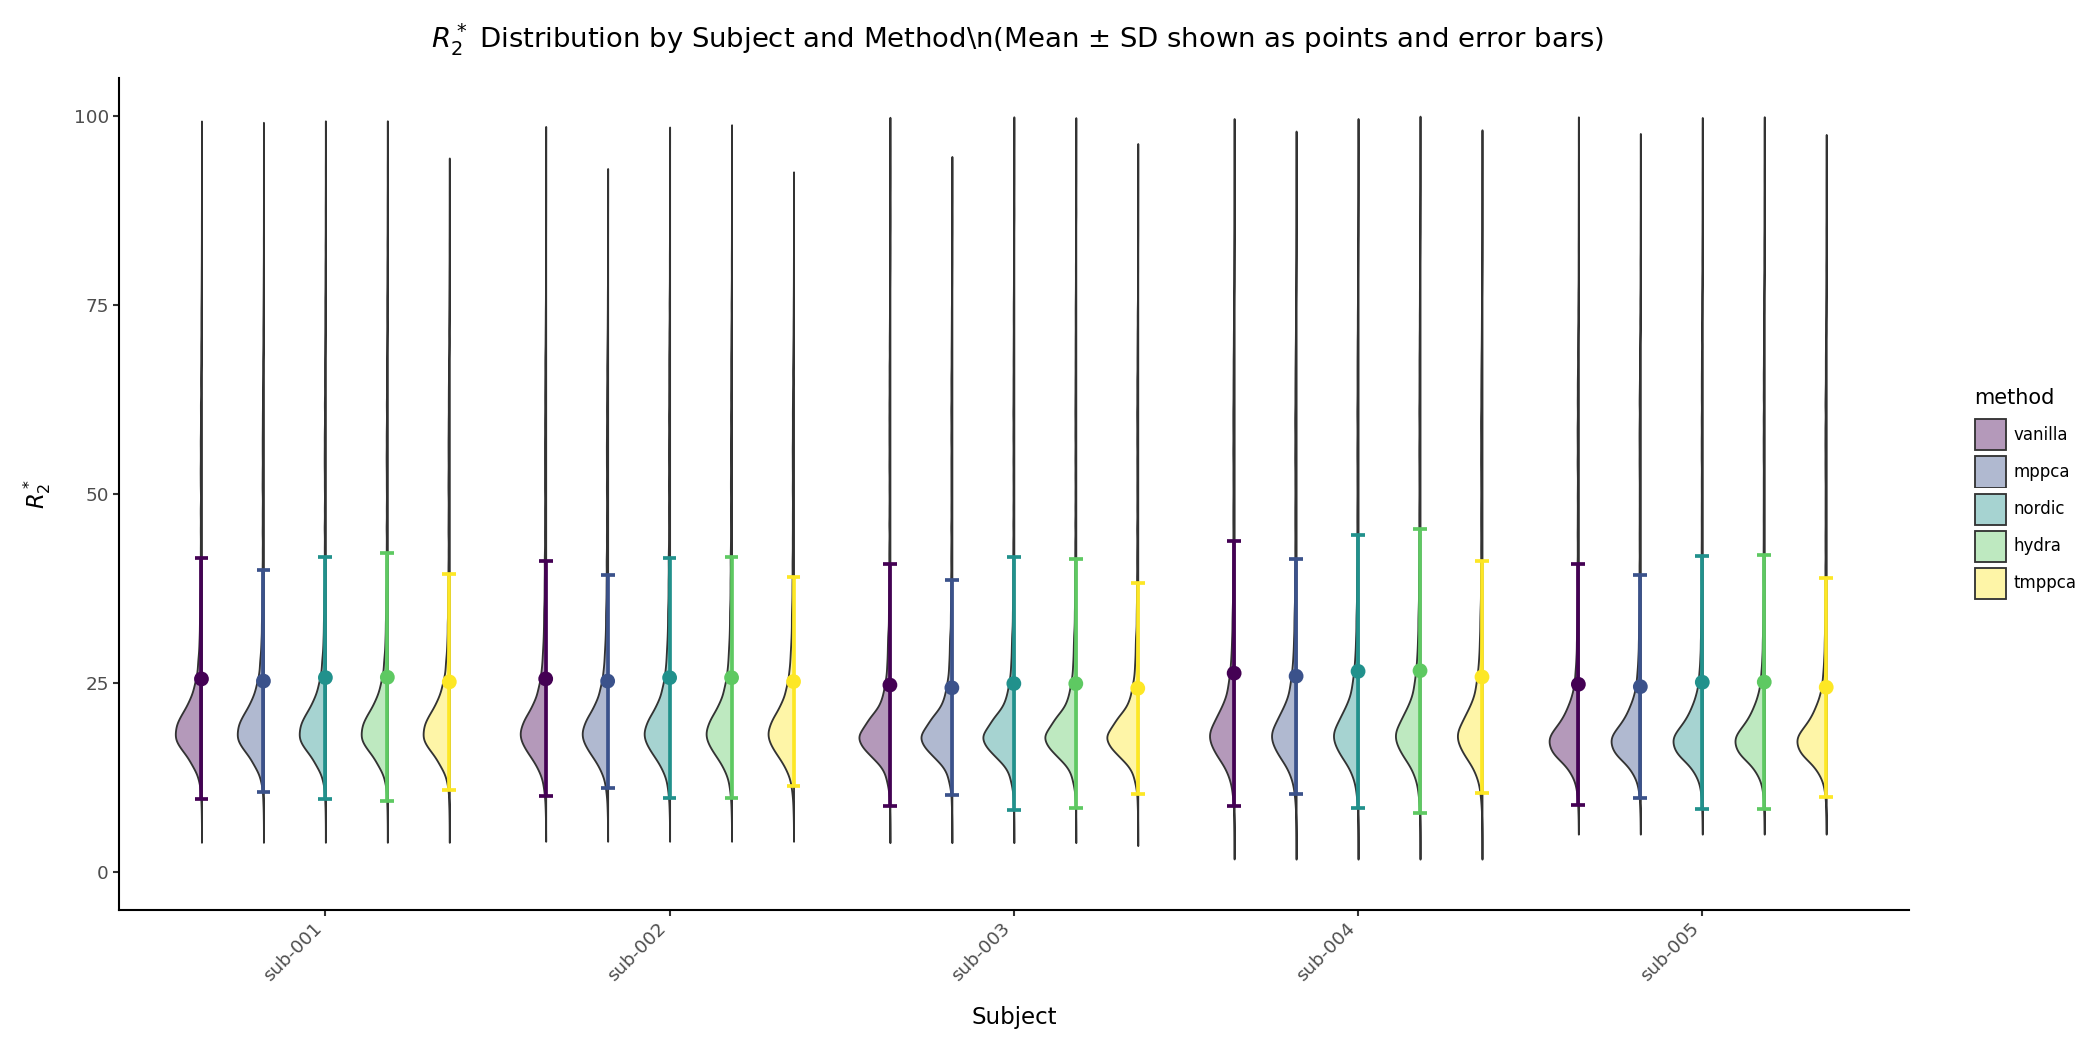
\includegraphics[width=10cm]{images/halfviolin_r2star_across_subjects_masked1200.png}\\
       \rotatebox[origin=l]{90}{\textcolor{black}{2 mm}} & 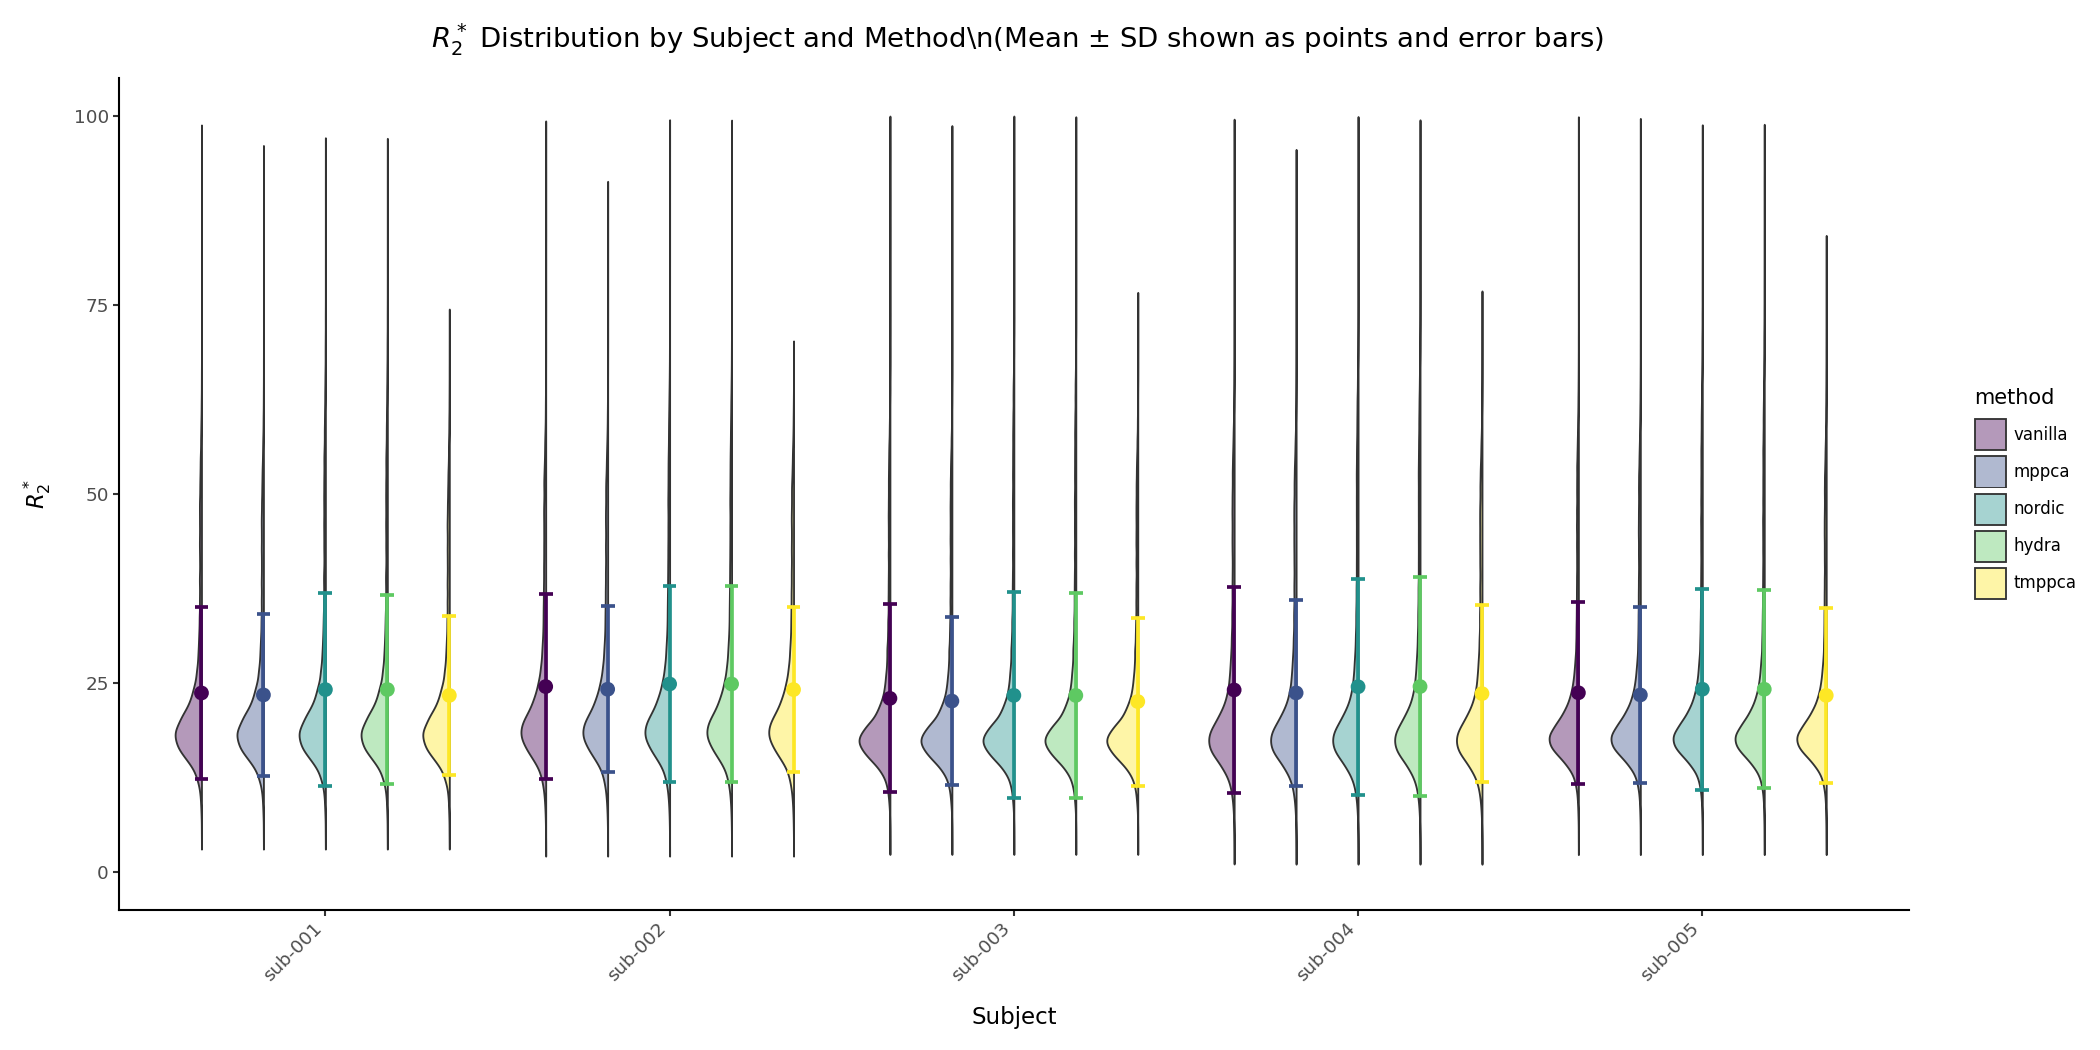
\includegraphics[width=10cm]{images/halfviolin_r2star_across_subjects_masked1700.png}\\
      \rotatebox[origin=l]{90}{\textcolor{black}{1.5 mm}}&   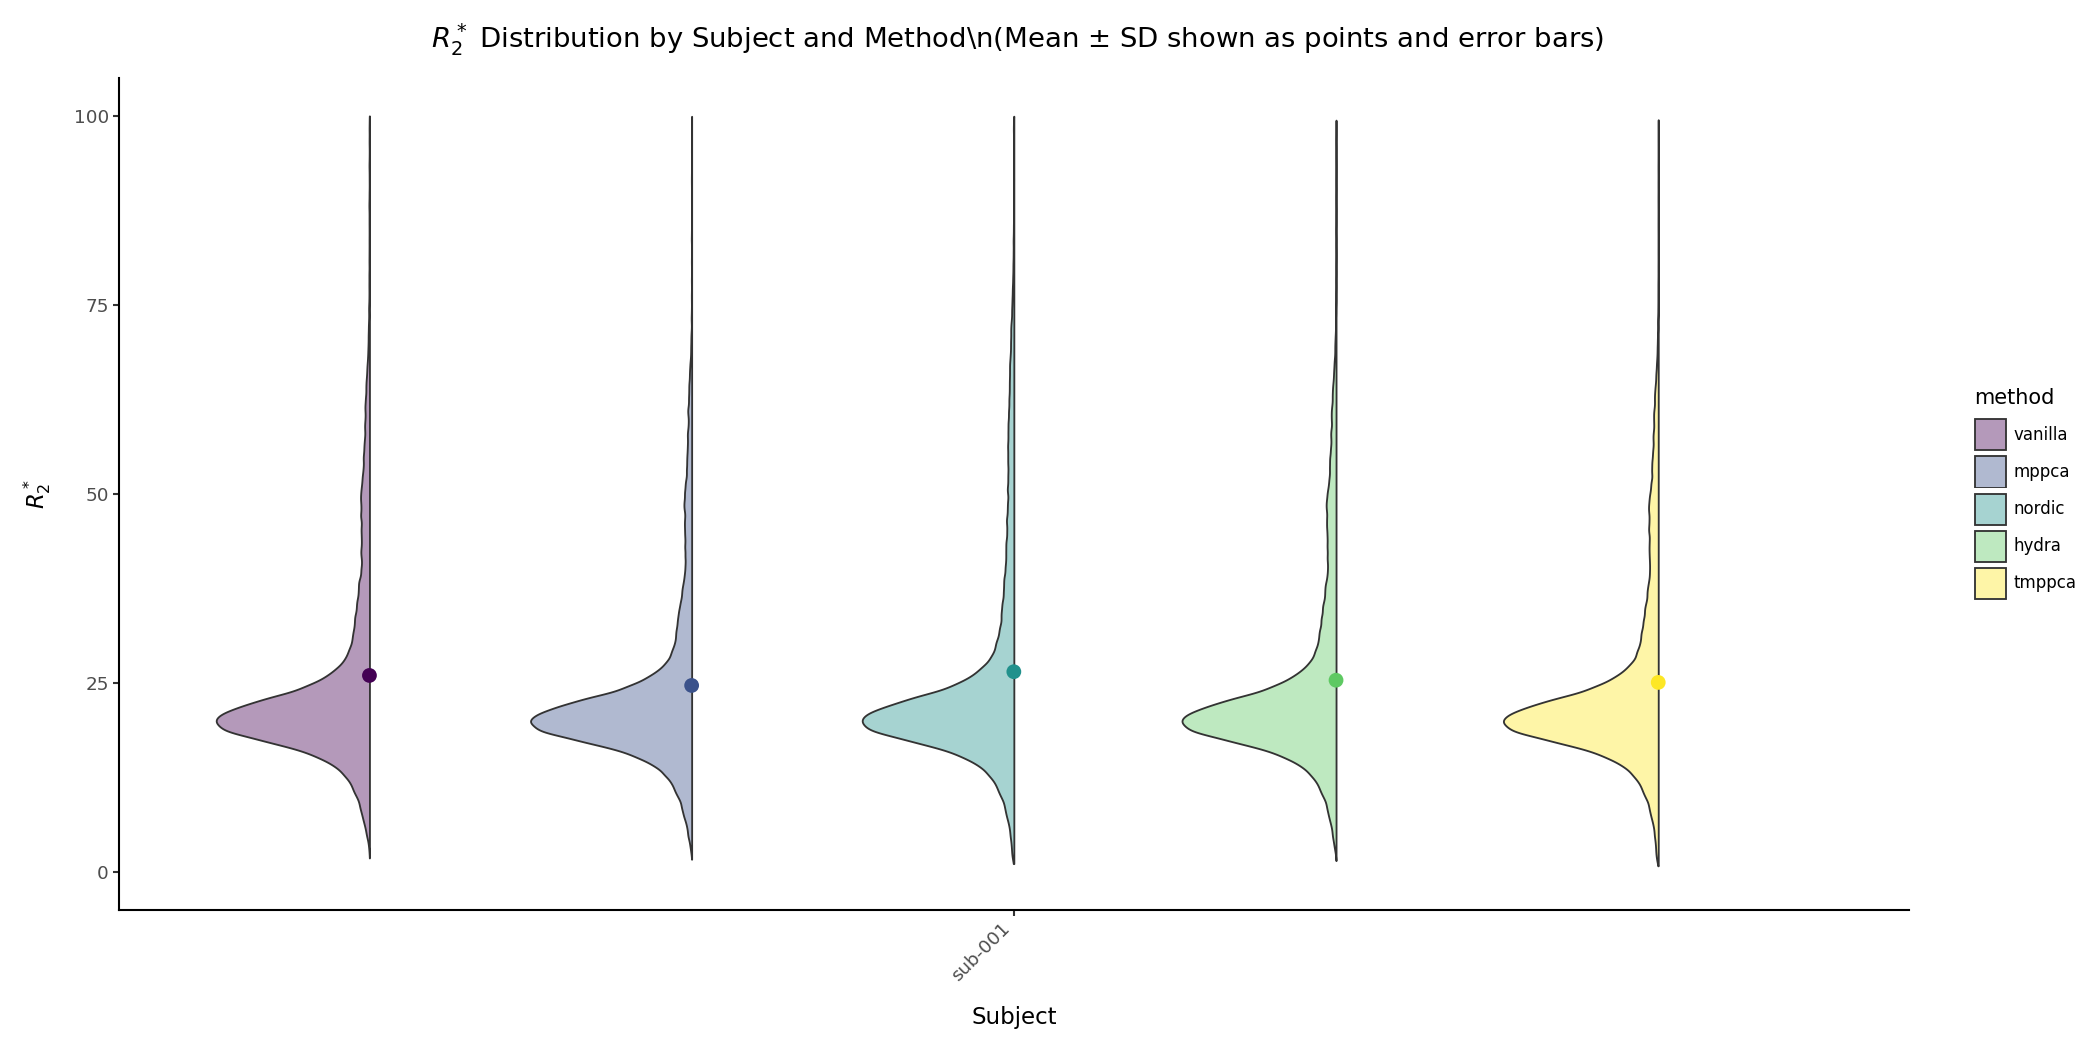
\includegraphics[width=10cm]{images/halfviolin_r2star_across_subjects_maskedHR.png}   \\
    \end{tabular}
    }
    \centering
    \caption[Distribution of $\overline{R_2^*}$ values per dataset]{Distribution of $\overline{R_2^*}$ values per dataset. Across all datasets, $\overline{R_2^*}$ distributions are largely similar between denoised and undenoised data, suggesting that the methods primarily remove variance of non-interest without affecting the $\overline{R_2^*}$ baseline.}
    \label{fig:R2mean}
\end{figure}
%-- Delta R2
\begin{figure}[htbp]
\centering \colorbox{white}{
    \centering
    \begin{tabular}{>{\centering\arraybackslash}m{.2cm}>{\centering\arraybackslash}m{5.5cm}>{\centering\arraybackslash}m{6cm}}
       & \textcolor{black}{\textbf{$\Delta R_2^*$}} & \textcolor{black}{\textbf{Plausible vs. Implausible}} \\
    \rotatebox[origin=l]{90}{\textcolor{black}{2.4 mm}} &    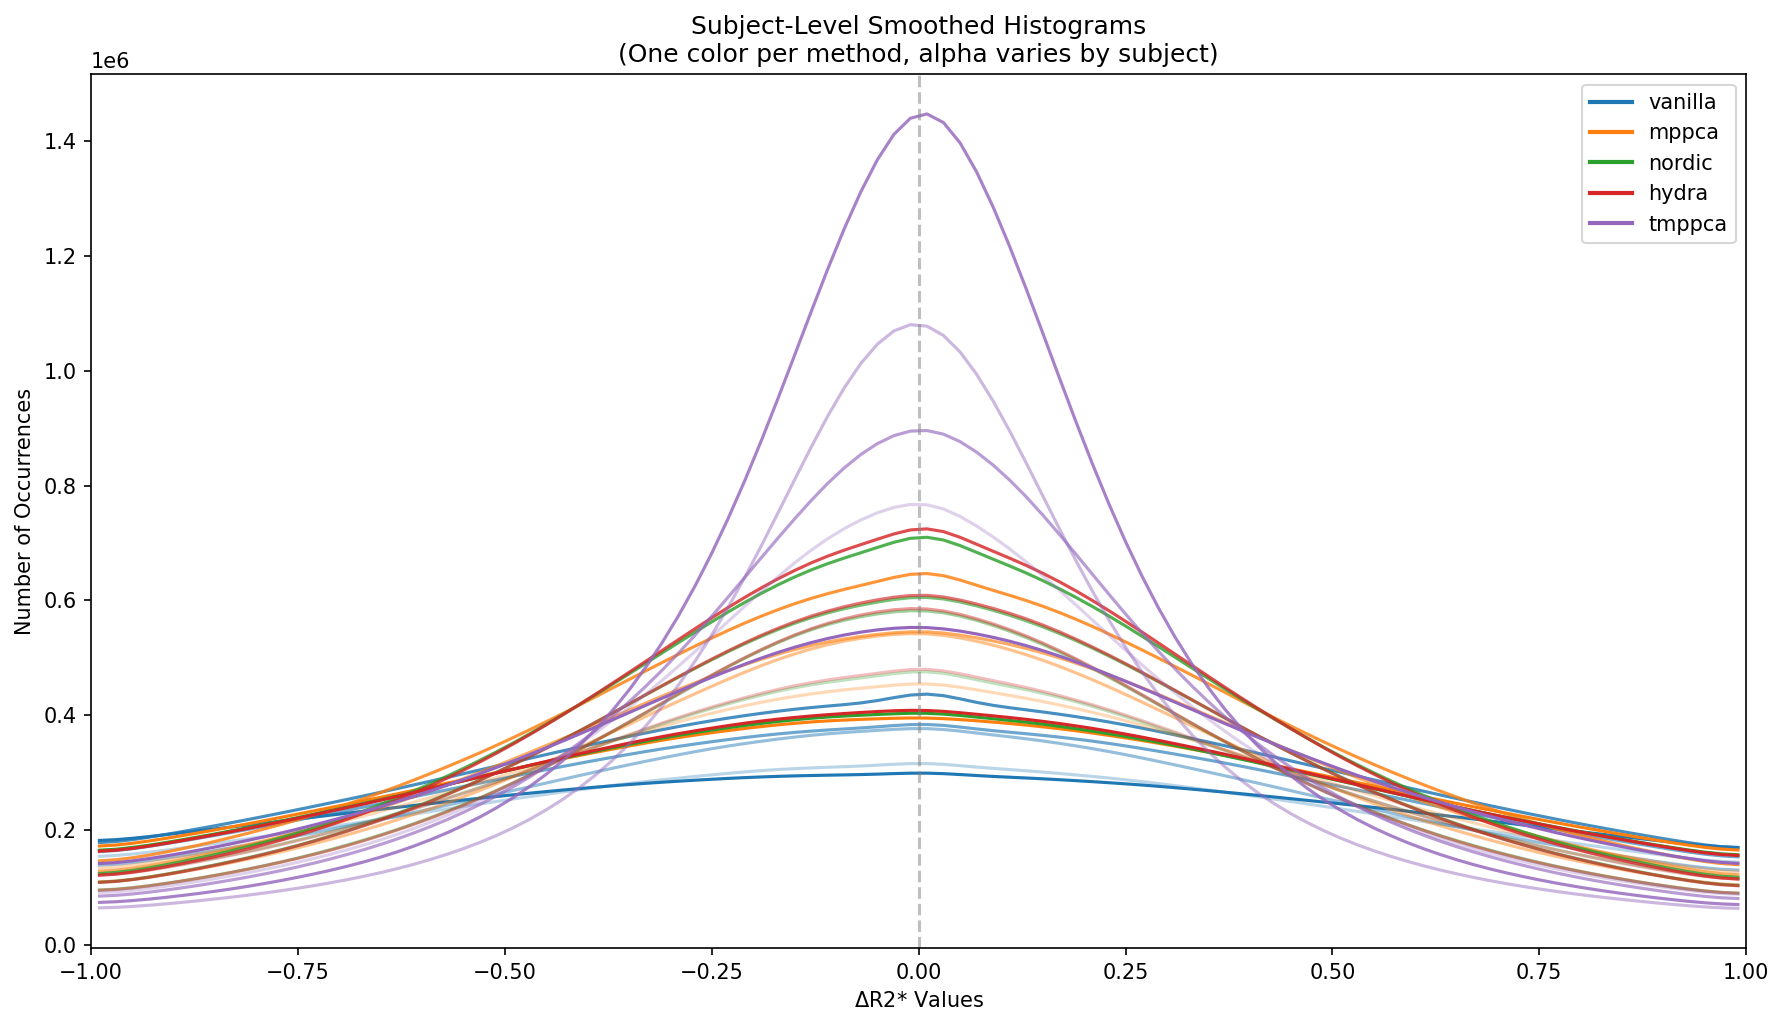
\includegraphics[width=6cm]{images/subject_smoothed_histograms1200.png} &
        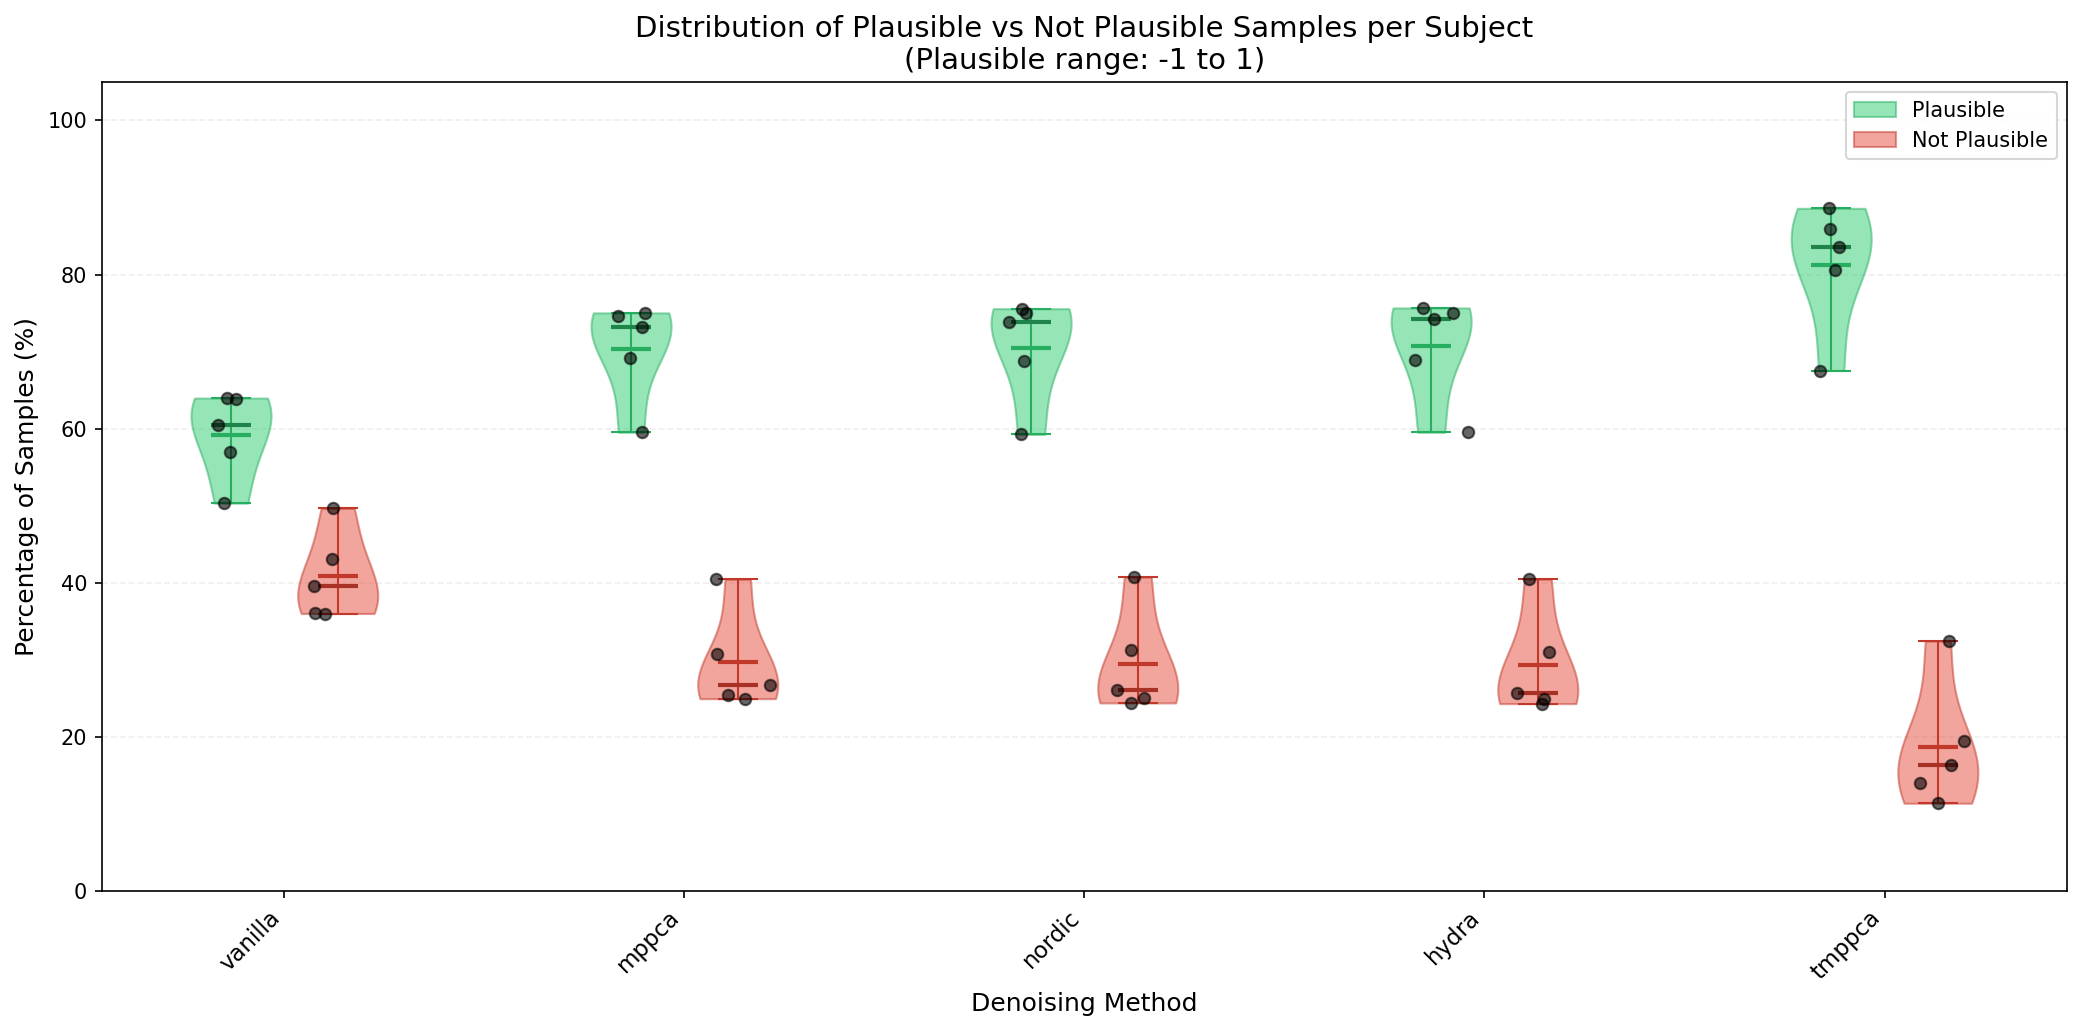
\includegraphics[width=5cm]{images/plausibility_paired_violin1200.png}\\
       \rotatebox[origin=l]{90}{\textcolor{black}{2 mm}} & 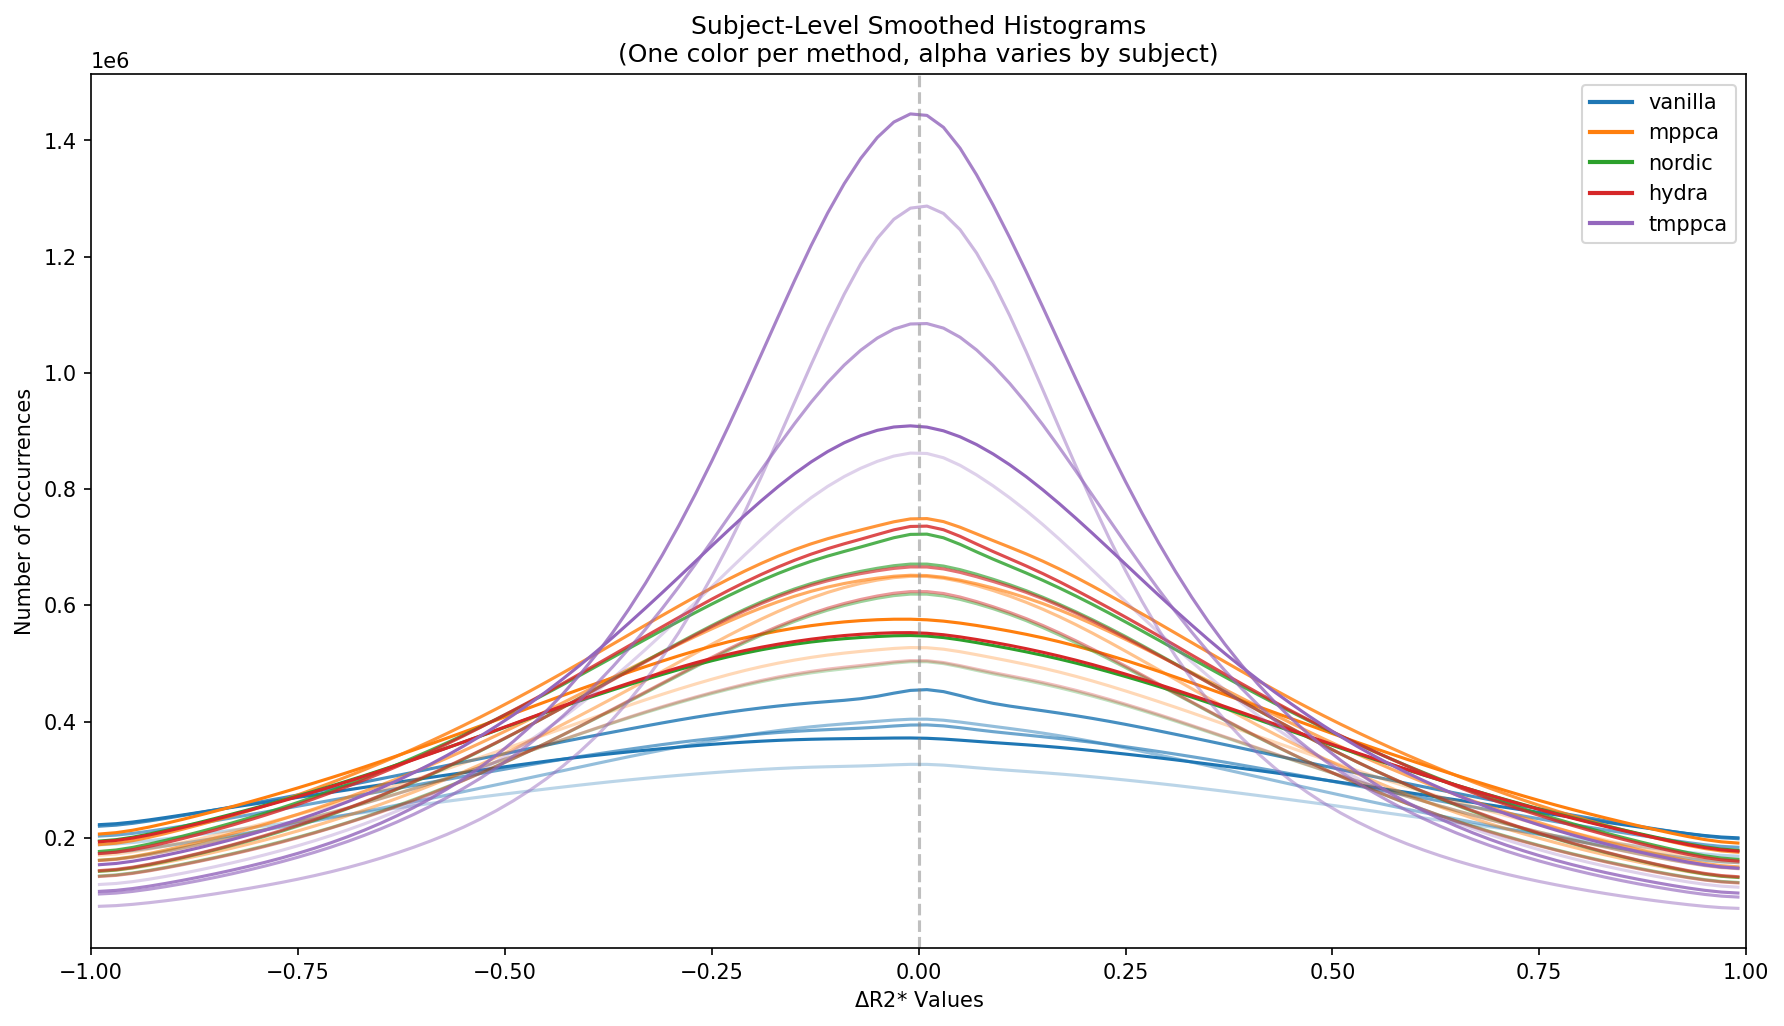
\includegraphics[width=6cm]{images/subject_smoothed_histograms1700.png}&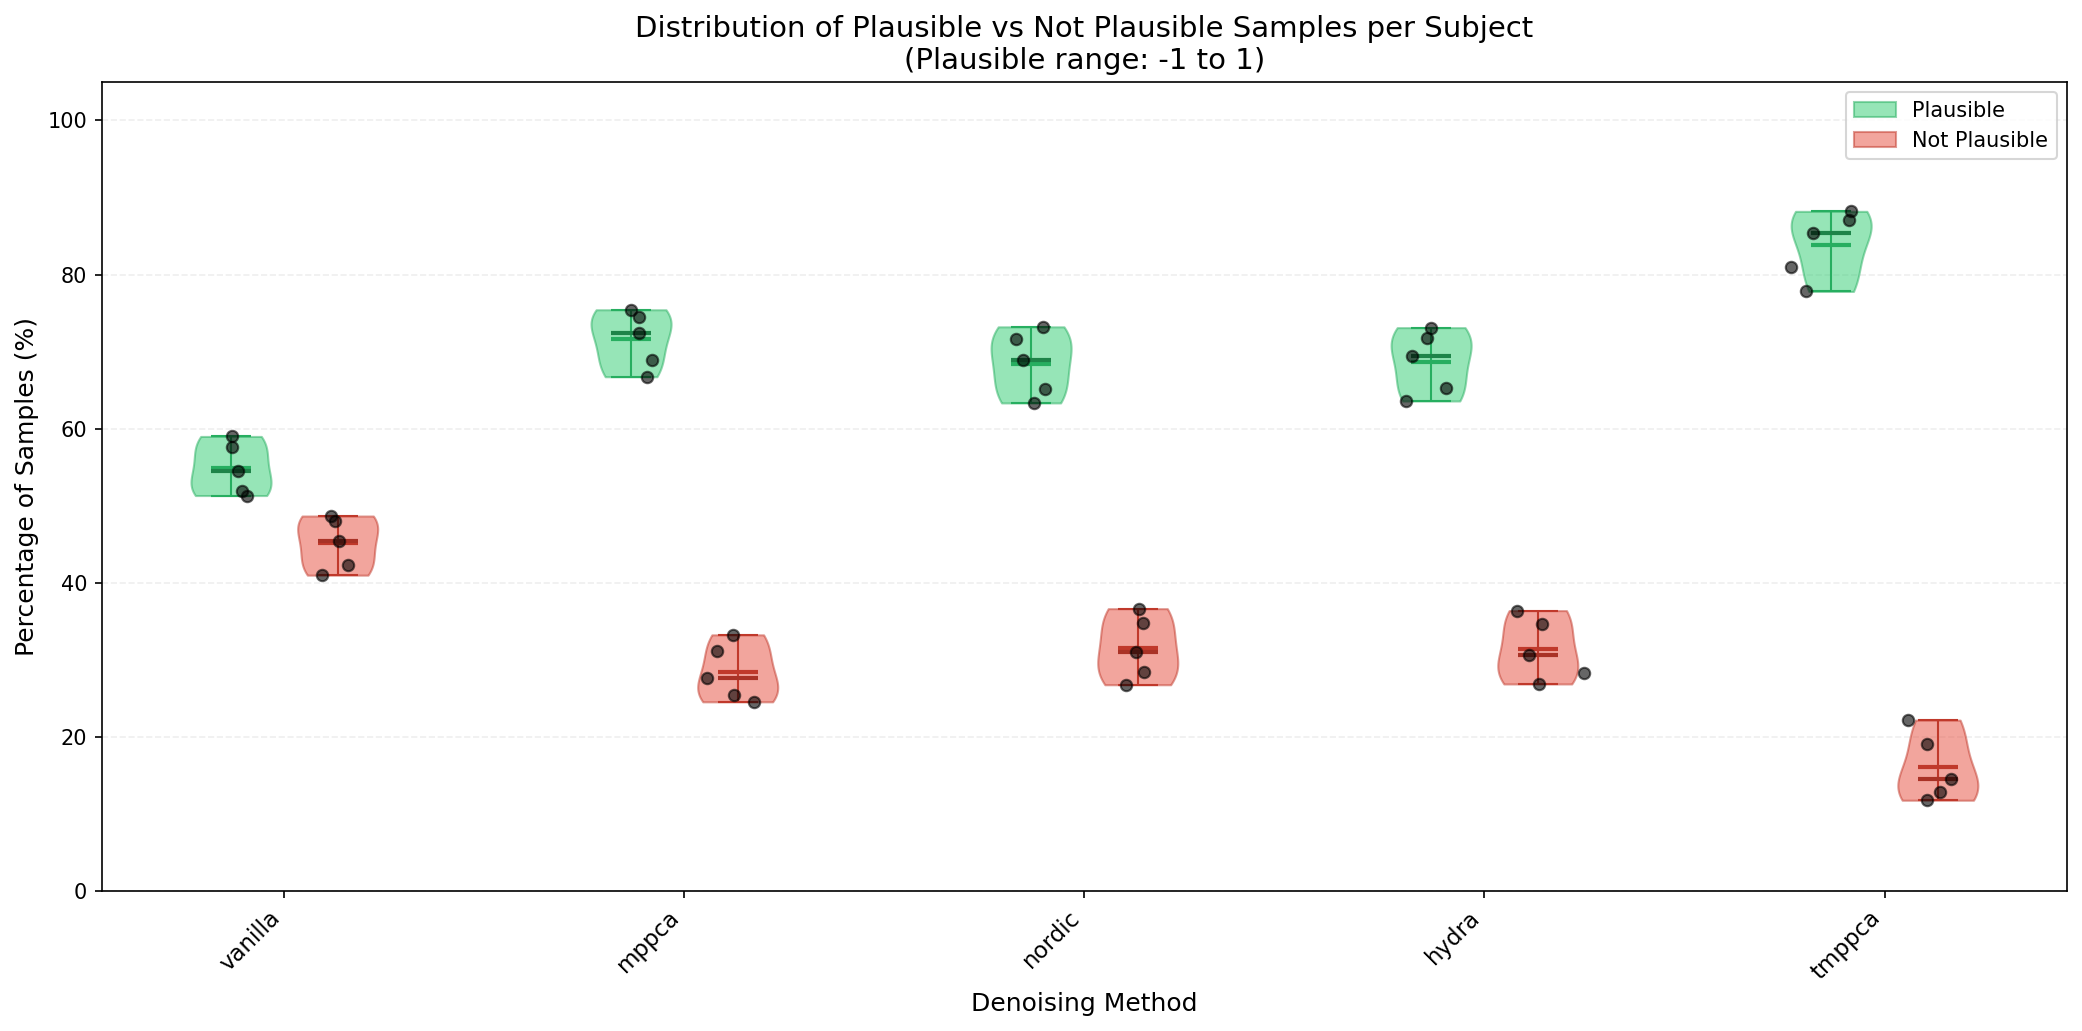
\includegraphics[width=5cm]{images/plausibility_paired_violin1700.png} \\
      \rotatebox[origin=l]{90}{\textcolor{black}{1.5 mm}}&   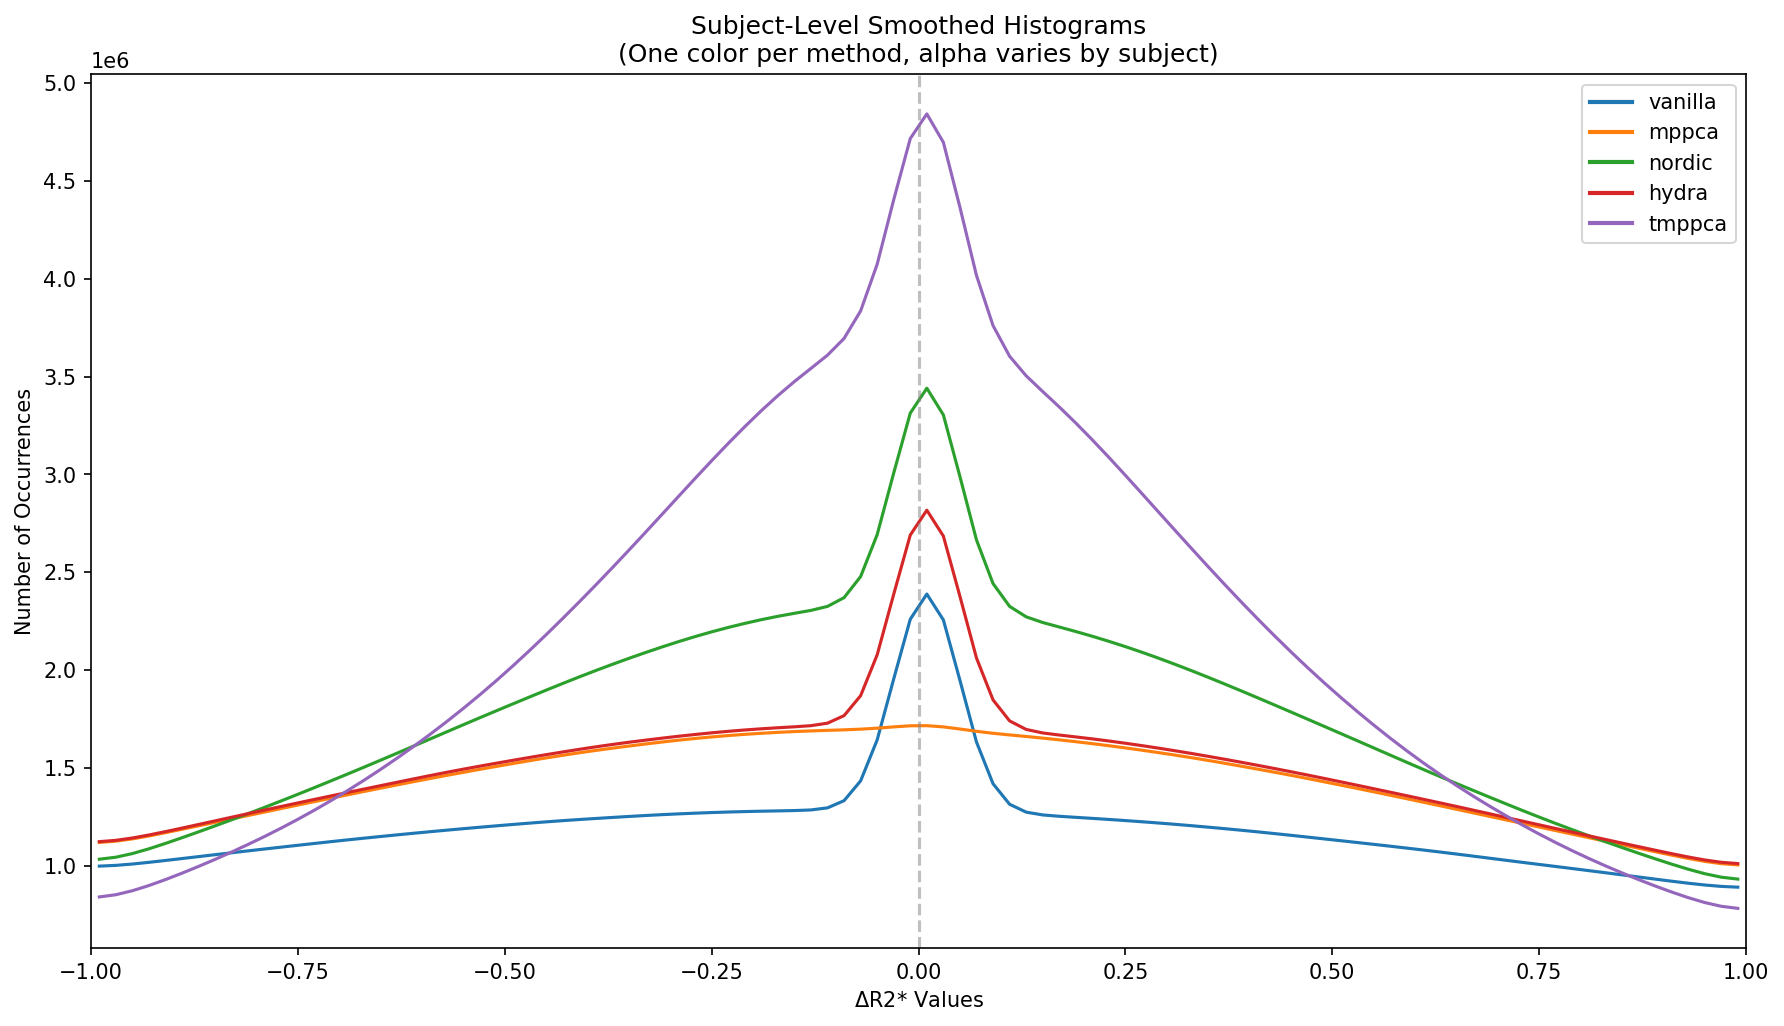
\includegraphics[width=6cm]{images/subject_smoothed_histogramsHR.png}&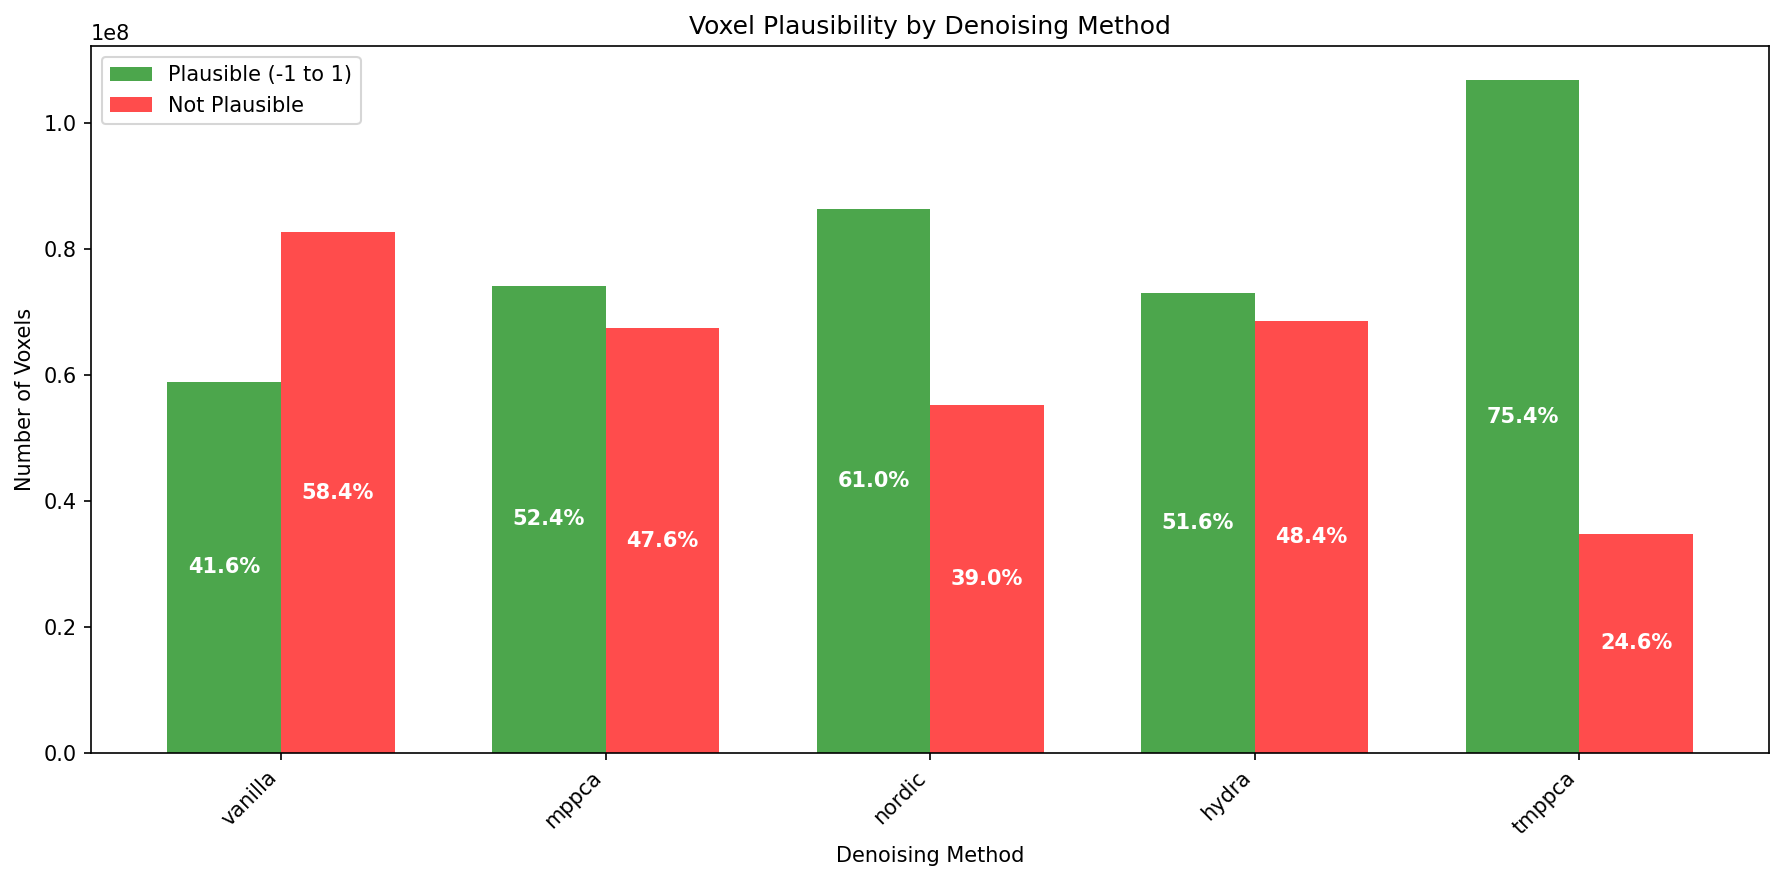
\includegraphics[width=5cm]{images/plausibility_paired_violinHR.png} \\
    \end{tabular}
    }
    \centering
    \caption[Distribution of $\Delta R_2^*$ values per dataset]{Distribution of $\Delta R_2^*$ values per dataset versus $\overline{R_2^*}$. Left: Smoothed histograms within the biologically plausible interval $[-1, 1]$ s (hemodynamic lag). For the low resolution (2.4 mm and 2 mm) datasets, each color-coded line corresponds to one subject. Right: Binary classification – plausible (green) vs. implausible (red).}
    \label{fig:plausabilityR2}
\end{figure}

To assess whether thermal denoising affects the physiological plausibility of the fMRI signal, we performed a $\overline{R_2^*}$ analysis. Given that fMRI relies on changes in $T_2^*$ decay, accurately estimating relaxation times is critical for detecting BOLD signal changes. We first sought to determine whether $\overline{R_2^*}$ estimates differed across denoising methods. If a denoising technique removes only random variance arising from thermal sources, the resulting $\overline{R_2^*}$ estimates should remain comparable to those obtained from the original data (i.e. vanilla approach). Consequently, evidence of changes in $\overline{\Delta R_2^*}$ relative to the original $\overline{\Delta R_2^*}$ would indicate that the overall signal range has been altered, suggesting the addition or removal of signal components.

Across the three datasets (2.4 mm, Fig.~\ref{fig:R21200}; 2 mm, Fig.~\ref{fig:R21700}; and 1.5 mm, Fig.~\ref{fig:R2HR}), changes in $\overline{R_2^*}$ were almost negligible (Fig.~\ref{fig:R2mean}), although NORDIC slightly overestimated $\overline{R_2^*}$ in low SNR areas, whereas TMPPCA and MPPCA tended to slightly underestimate it. HYDRA, consistent with the tSNR findings, showed a pattern similar to NORDIC in the high SNR dataset, while more closely resembling MPPCA in the low SNR dataset. In general, discrepancies with respect to the vanilla $\overline{R_2^*}$ estimates were most pronounced in orbitofrontal, anterior frontal and inferior temporal regions that exhibit large signal dropouts and susceptibility effects.

We next conducted a more fine-grained analysis of temporal changes in relaxation times. Such fluctuations may reflect hemodynamic processes if their characteristics are physiologically  plausible lags of a fast hemodynamic response function, such as those typically observed in BOLD responses (Fig.~\ref{fig:plausabilityR2}) \citep{uludagIntegrativeModelNeuronal2009a, uludagLinkingBrainVascular2018, dezwartTemporalDynamicsBOLD2005}. Overall, TMPPCA yielded a larger number of data points within the biologically plausible range, suggesting that the variance removed by TMPPCA predominantly reflects non-neuronal or otherwise non-interest signal components. As shown in the right panel of Fig.~\ref{fig:plausabilityR2}, all denoising strategies increase the proportion of samples with plausible $R_{2}^{*}$ estimates relative to the undenoised data (vanilla condition). Again, TMPPCA produces the largest improvement and clearly outperforms the other approaches, and the advantages of TMPPCA over the other denoising methods became more pronounced as voxel resolution increased. NORDIC constitutes the second most effective strategy in this regard. Notably, NORDIC and HYDRA did not demonstrate a clear advantage over MPPCA in this regard.


Collectively, these findings indicate that TMPPCA not only improves the tSNR of multi-echo fMRI datasets but does so in a physiologically plausible manner. This provides confidence that the enhanced signal quality reflects genuine changes in brain tissue magnetization, likely arising from hemodynamic processes.



%%%%%%-------
% -----------S 0
% -----------
%%%%%%-------

\begin{figure}[htbp]
\centering \colorbox{black}{
    \centering
    \begin{tabular}{>{\centering\arraybackslash}m{.7cm}>{\centering\arraybackslash}m{3cm}>{\centering\arraybackslash}m{3cm}>{\centering\arraybackslash}m{.7cm}}
    
       & \textcolor{white}{\textbf{$S_0$}} & \textcolor{white}{\textbf{$\Delta S_0$}}& \\
   \rotatebox[origin=l]{90}{\textcolor{white}{VANILLA}}
  &    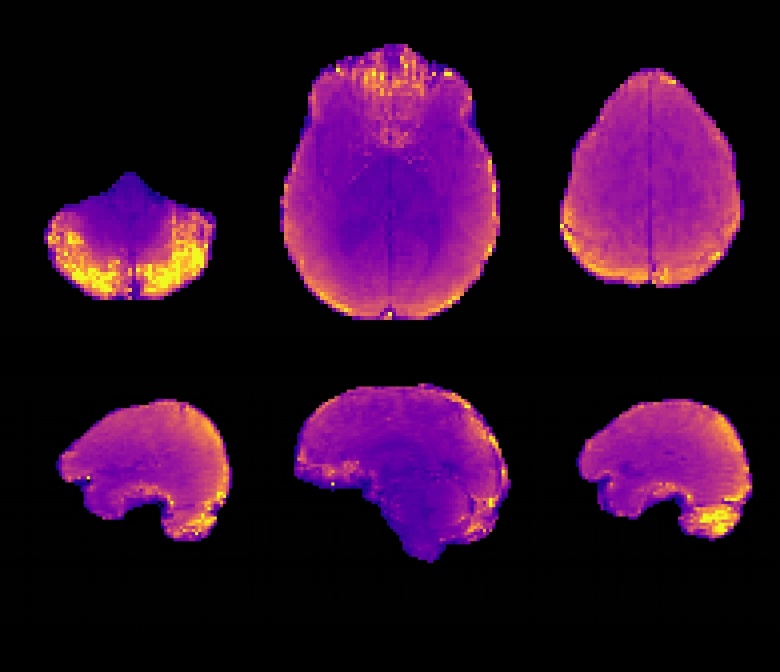
\includegraphics[width=3cm]{images/sub-001_ses-1_task-HABLA1200_S0mean_part-mag_bold_vanilla_all.jpg} & & \textcolor{white}{$S_0$} 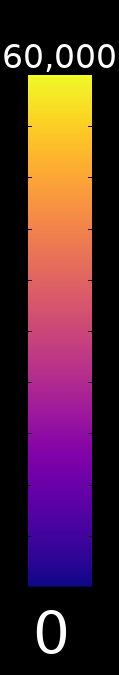
\includegraphics[width=.5cm]{images/Plasmas0.png}\\
     \rotatebox[origin=l]{90}{\textcolor{white}{MPPCA}}
  &    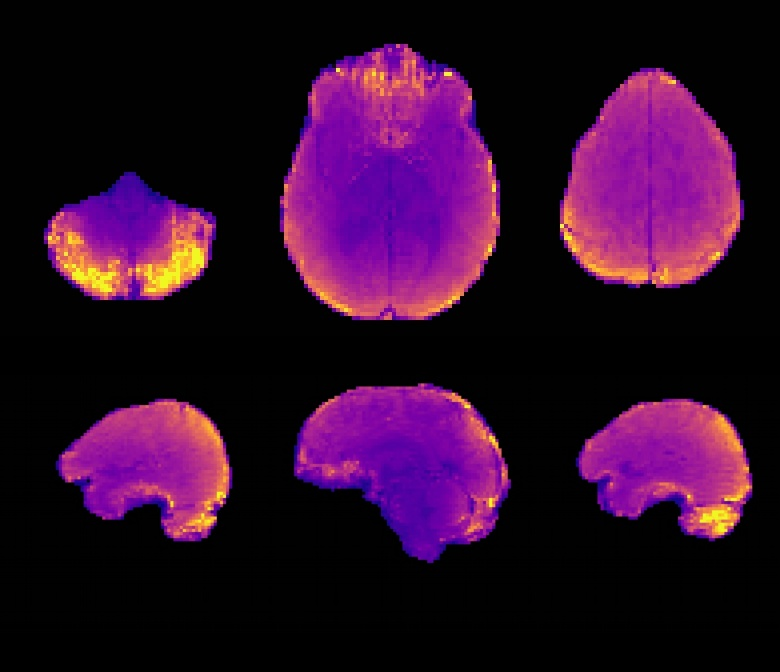
\includegraphics[width=3cm]{images/sub-001_ses-1_task-HABLA1200_S0mean_part-mag_bold_mppca_all} &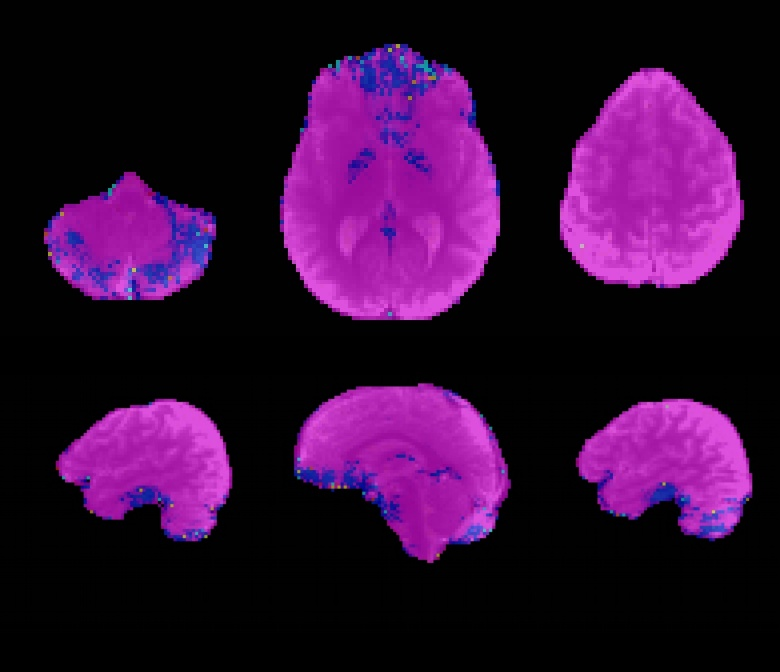
\includegraphics[width=3cm]{images/sub-001_ses-1_task-HABLA1200_S0meanSPC_part-mag_bold_mppca_all} &\\
       \rotatebox[origin=l]{90}{\textcolor{white}{NORDIC}}
  &    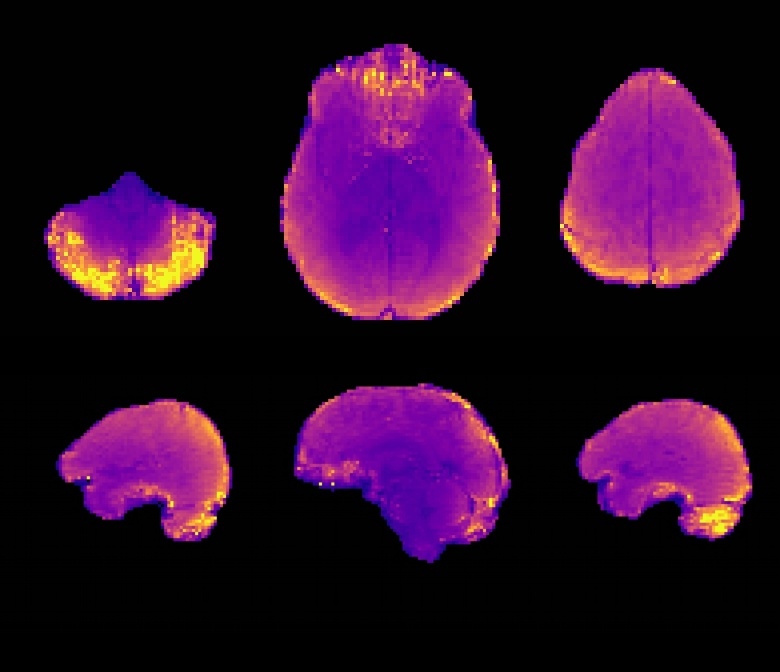
\includegraphics[width=3cm]{images/sub-001_ses-1_task-HABLA1200_S0mean_part-mag_bold_nordic_all.jpg} &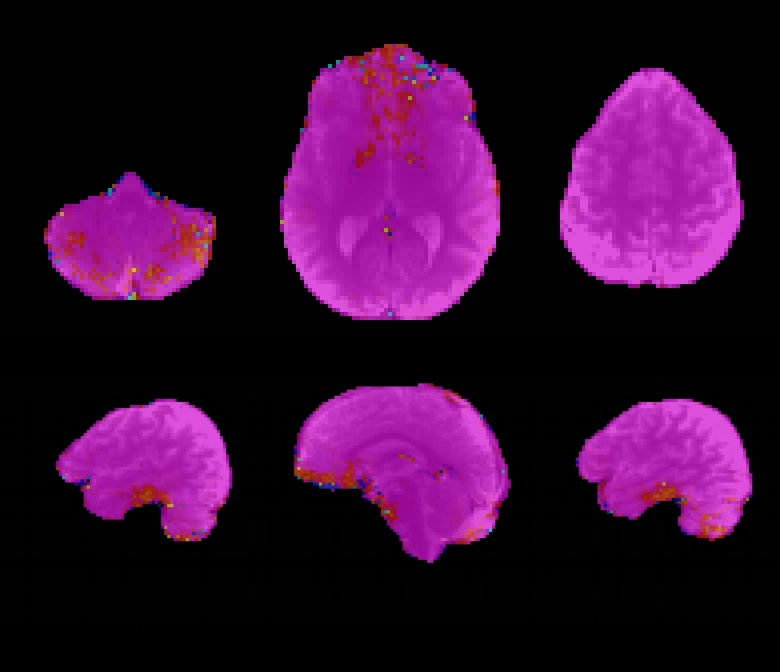
\includegraphics[width=3cm]{images/sub-001_ses-1_task-HABLA1200_S0meanSPC_part-mag_bold_nordic_all} &\\
       \rotatebox[origin=l]{90}{\textcolor{white}{HYDRA}}
  &    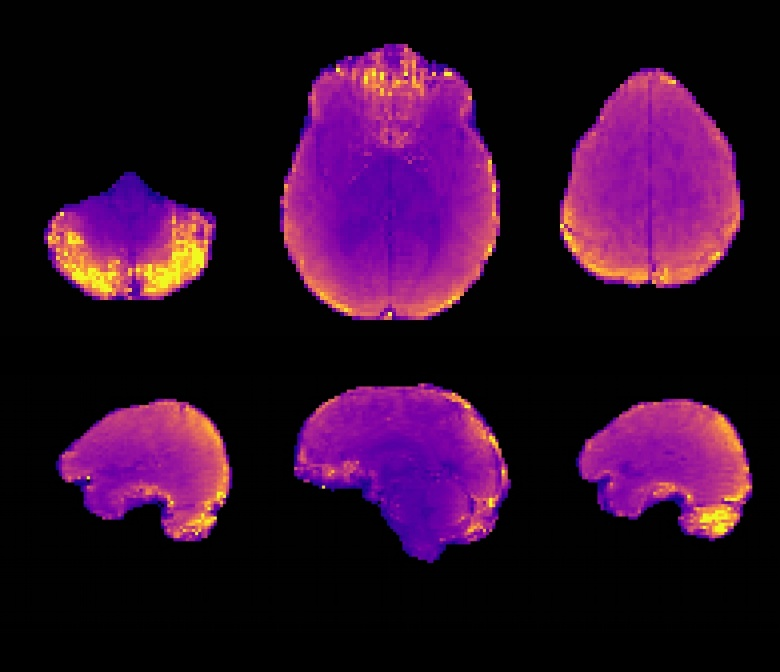
\includegraphics[width=3cm]{images/sub-001_ses-1_task-HABLA1200_S0mean_part-mag_bold_hydra_all.jpg} &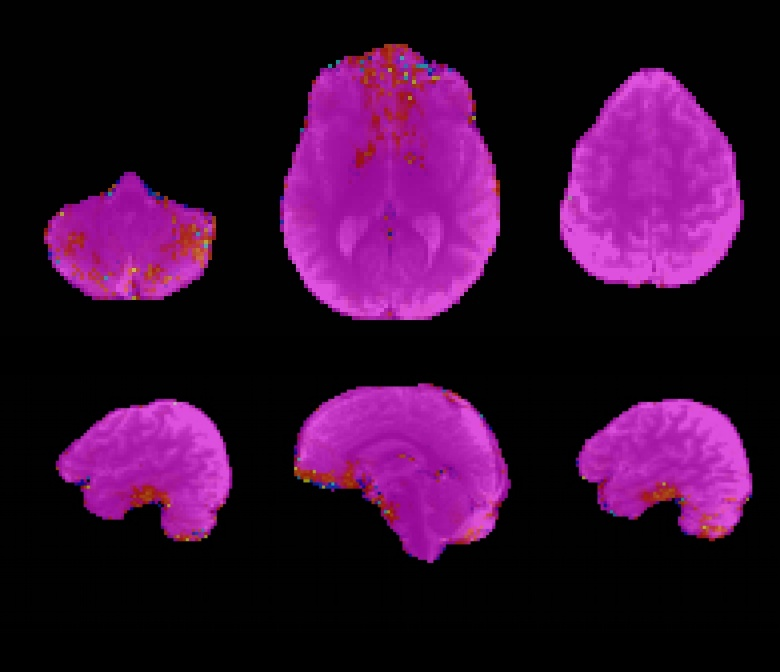
\includegraphics[width=3cm]{images/sub-001_ses-1_task-HABLA1200_S0meanSPC_part-mag_bold_hydra_all} &\\
       \rotatebox[origin=l]{90}{\textcolor{white}{TMPPCA}}
  &    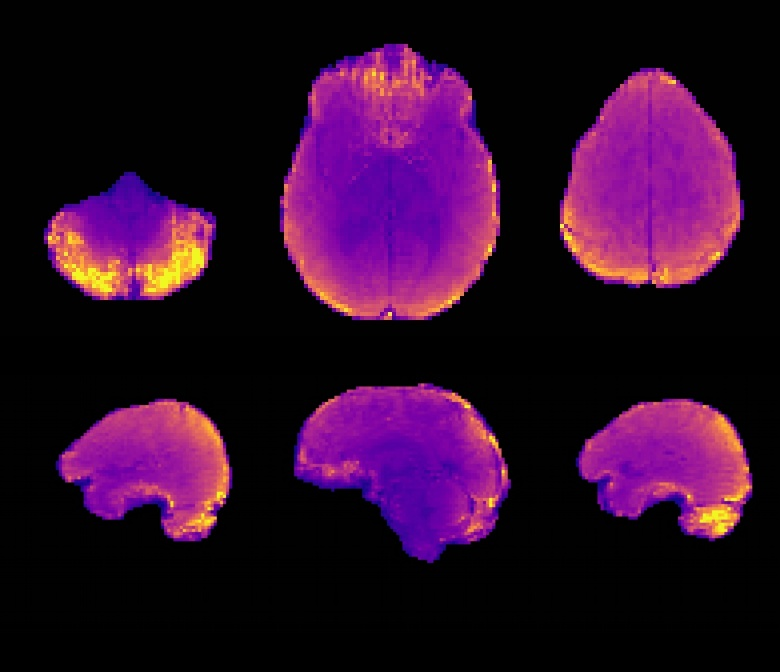
\includegraphics[width=3cm]{images/sub-001_ses-1_task-HABLA1200_S0mean_part-mag_bold_tmppca_all.jpg} &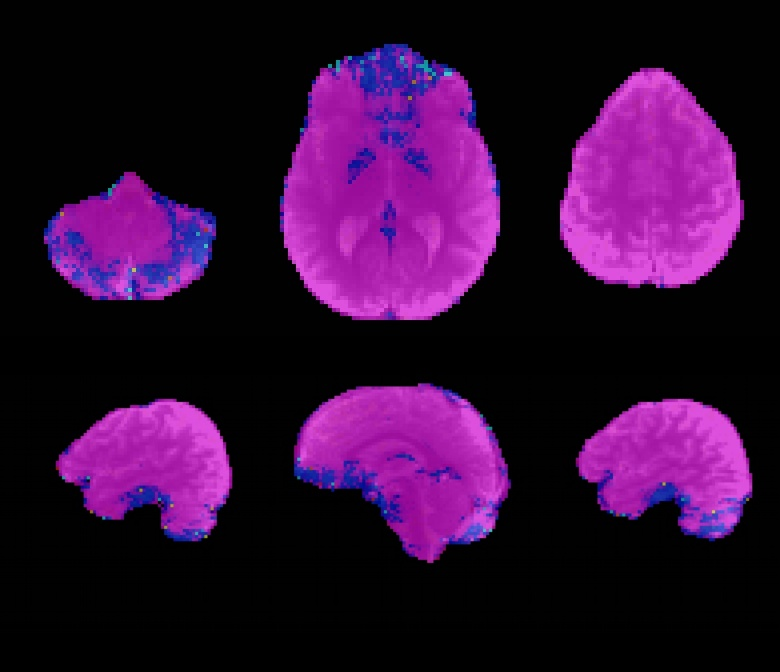
\includegraphics[width=3cm]{images/sub-001_ses-1_task-HABLA1200_S0meanSPC_part-mag_bold_tmppca_all} &\textcolor{white}{$\Delta S_0$} 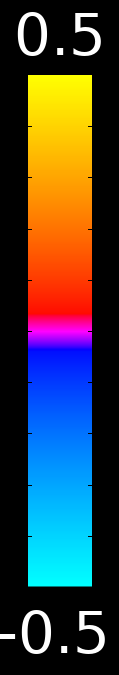
\includegraphics[width=.5cm]{images/SPC.png}\\
    \end{tabular}
    }
    \caption[$S_0^$ maps at low resolution (2.4 mm isotropic)]{Left: $S_0$ maps (2.4 mm). Right: $\Delta S_0$ (change relative to vanilla).}
    \label{fig:S01200}
\end{figure}

\begin{figure}[htbp]
\centering \colorbox{black}{
    \centering
    \begin{tabular}{>{\centering\arraybackslash}m{.7cm}>{\centering\arraybackslash}m{3cm}>{\centering\arraybackslash}m{3cm}>{\centering\arraybackslash}m{.7cm}}
    
       & \textcolor{white}{\textbf{$S_0$}} & \textcolor{white}{\textbf{$\Delta S_0$}}& \\
   \rotatebox[origin=l]{90}{\textcolor{white}{VANILLA}}
  &    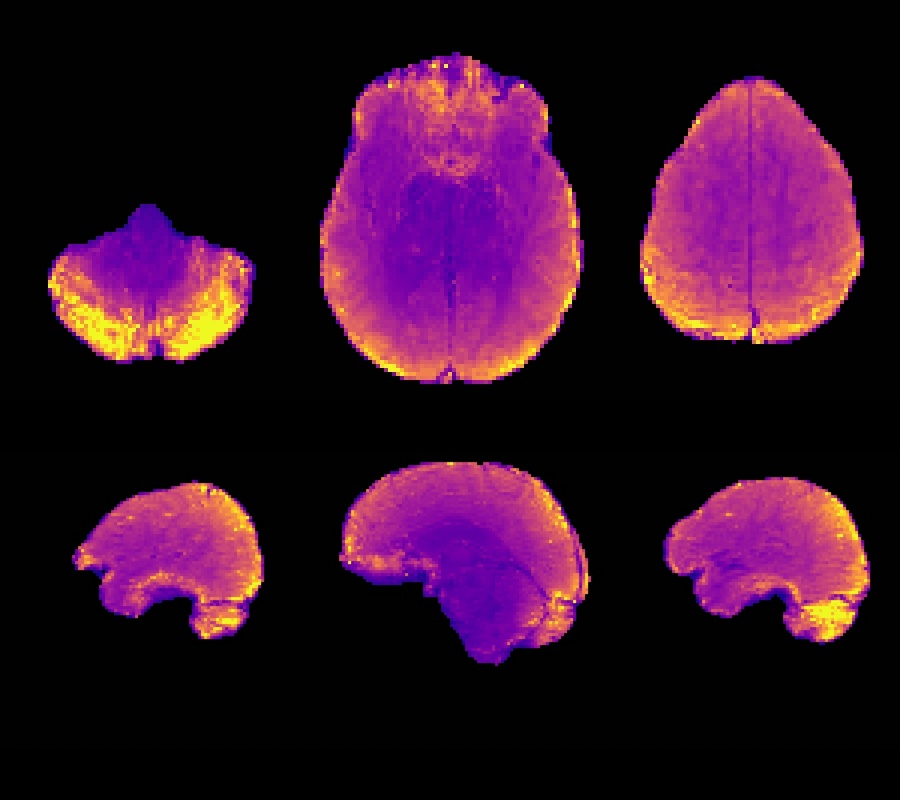
\includegraphics[width=3cm]{images/sub-001_ses-1_task-HABLA1700_S0mean_part-mag_bold_vanilla_all.jpg} & & \textcolor{white}{$S_0$} 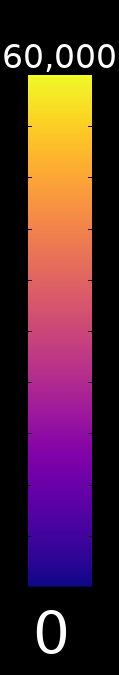
\includegraphics[width=.5cm]{images/Plasmas0.png}\\
     \rotatebox[origin=l]{90}{\textcolor{white}{MPPCA}}
  &    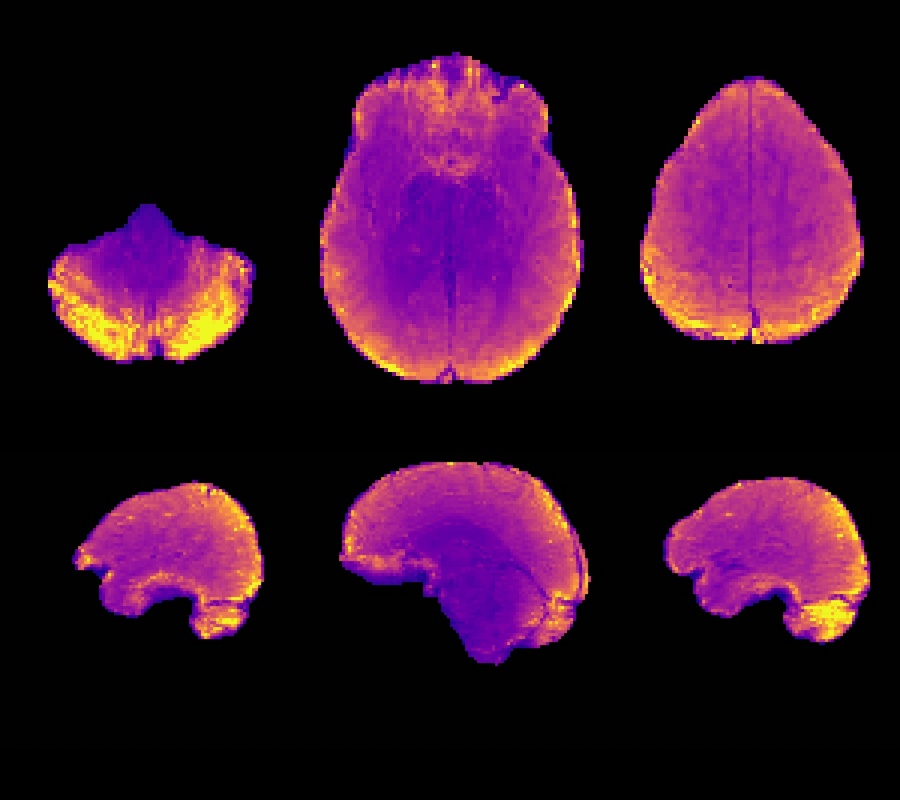
\includegraphics[width=3cm]{images/sub-001_ses-1_task-HABLA1700_S0mean_part-mag_bold_mppca_all} &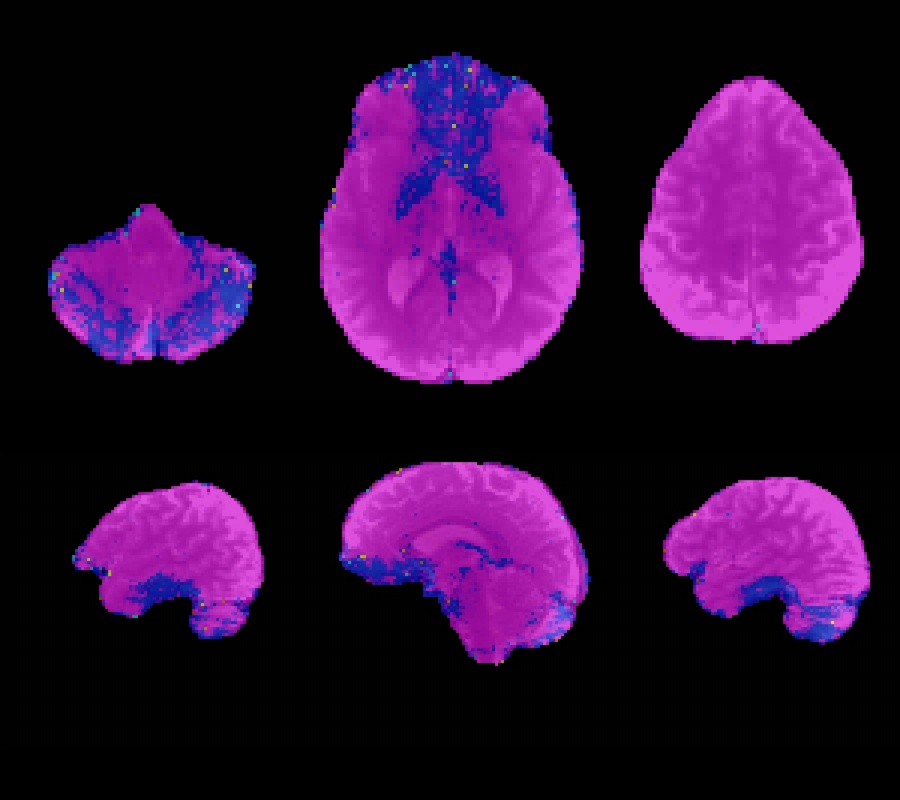
\includegraphics[width=3cm]{images/sub-001_ses-1_task-HABLA1700_S0meanSPC_part-mag_bold_mppca_all} &\\
       \rotatebox[origin=l]{90}{\textcolor{white}{NORDIC}}
  &    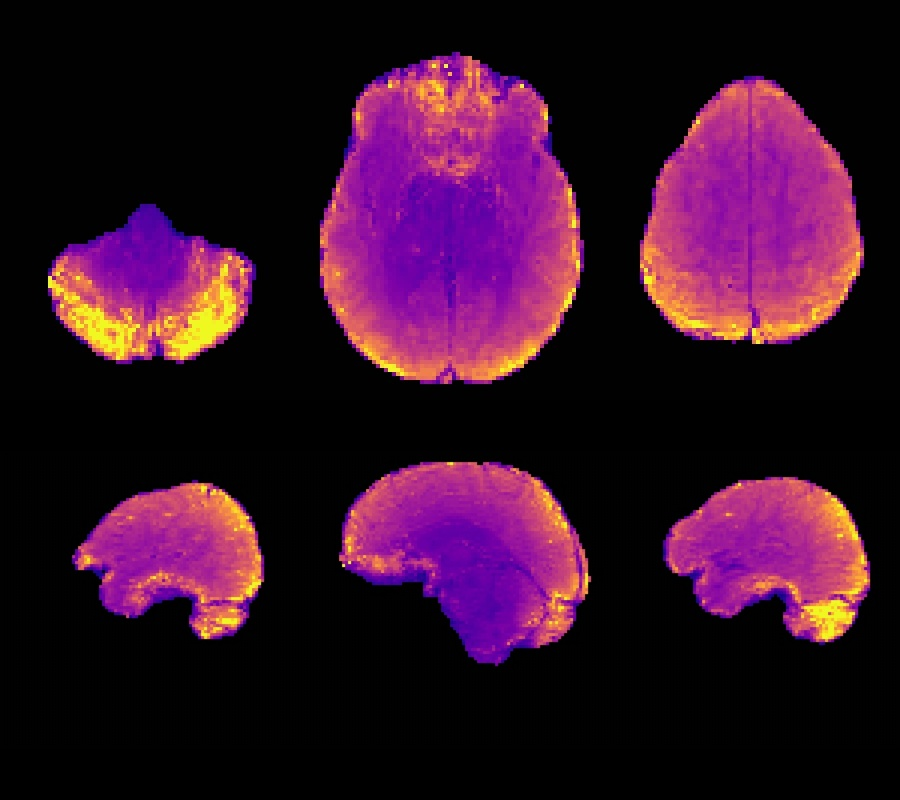
\includegraphics[width=3cm]{images/sub-001_ses-1_task-HABLA1700_S0mean_part-mag_bold_nordic_all.jpg} &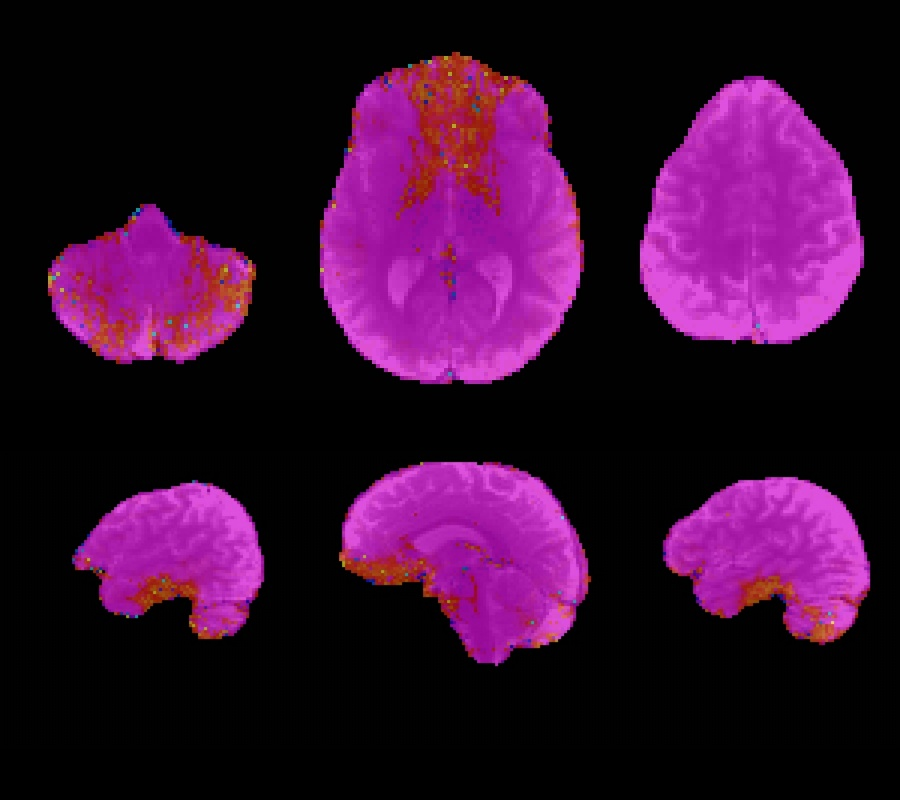
\includegraphics[width=3cm]{images/sub-001_ses-1_task-HABLA1700_S0meanSPC_part-mag_bold_nordic_all} &\\
       \rotatebox[origin=l]{90}{\textcolor{white}{HYDRA}}
  &    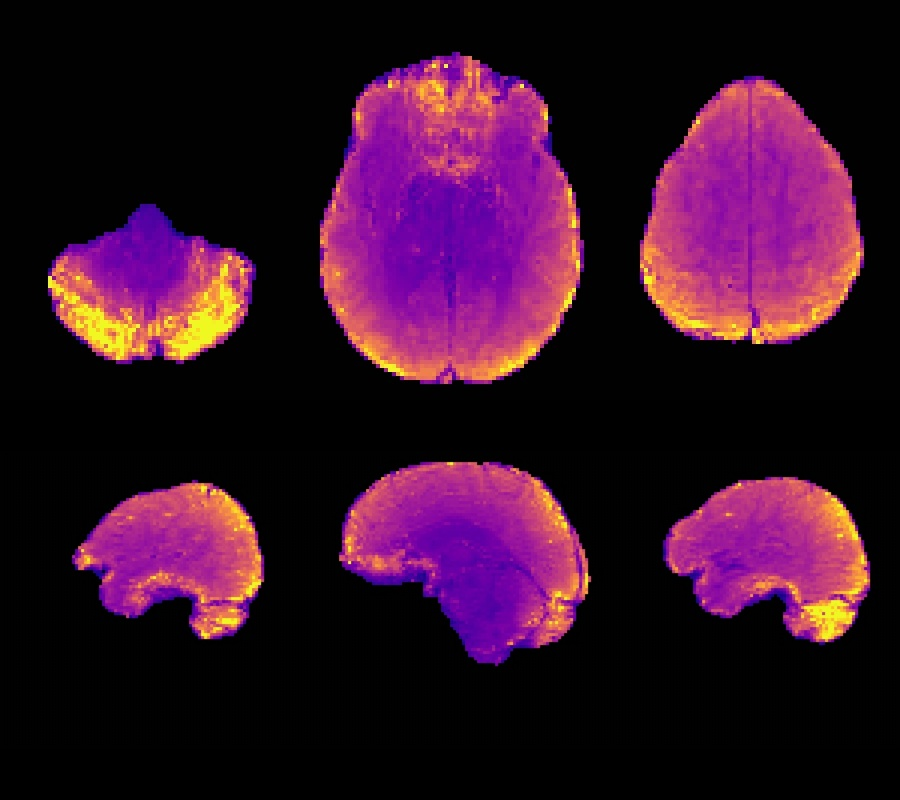
\includegraphics[width=3cm]{images/sub-001_ses-1_task-HABLA1700_S0mean_part-mag_bold_hydra_all.jpg} &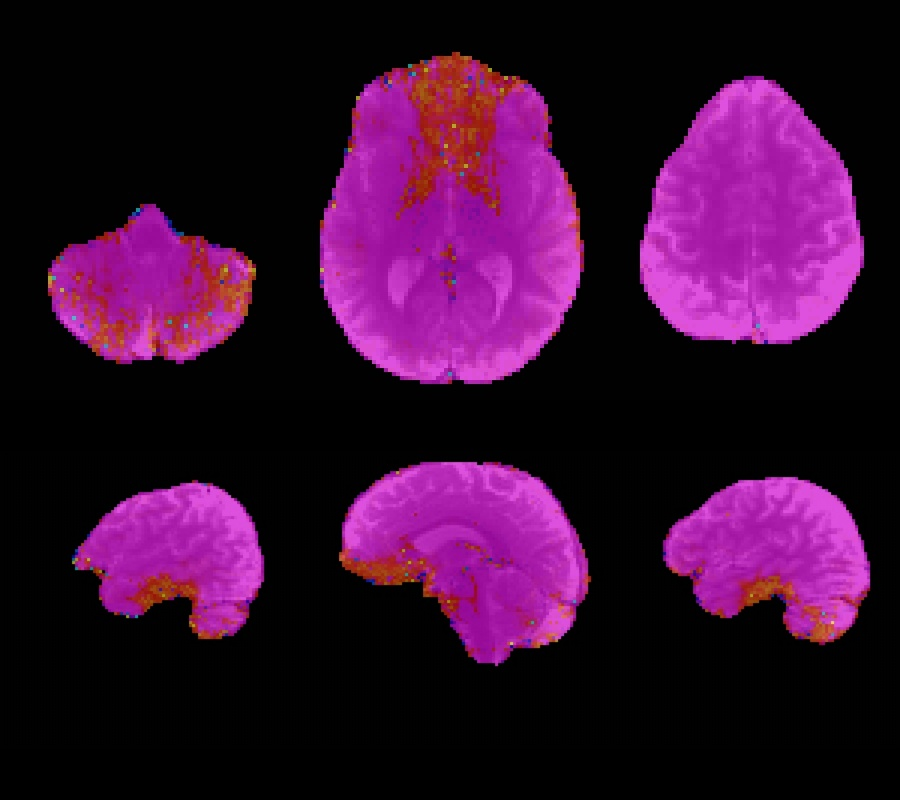
\includegraphics[width=3cm]{images/sub-001_ses-1_task-HABLA1700_S0meanSPC_part-mag_bold_hydra_all} &\\
       \rotatebox[origin=l]{90}{\textcolor{white}{TMPPCA}}
  &    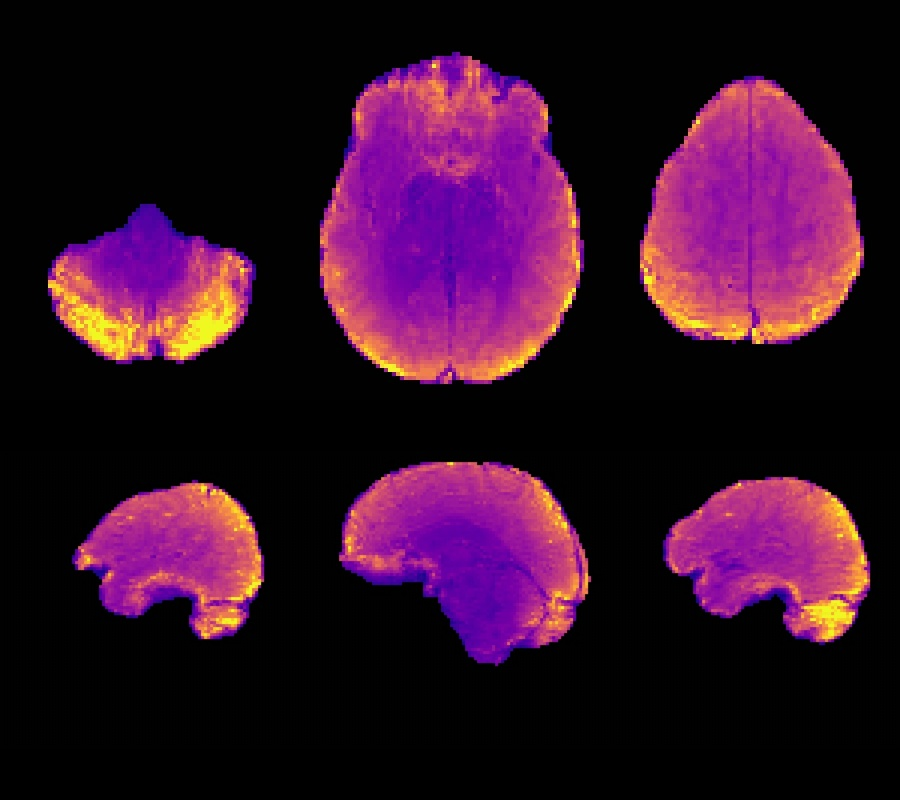
\includegraphics[width=3cm]{images/sub-001_ses-1_task-HABLA1700_S0mean_part-mag_bold_tmppca_all.jpg} &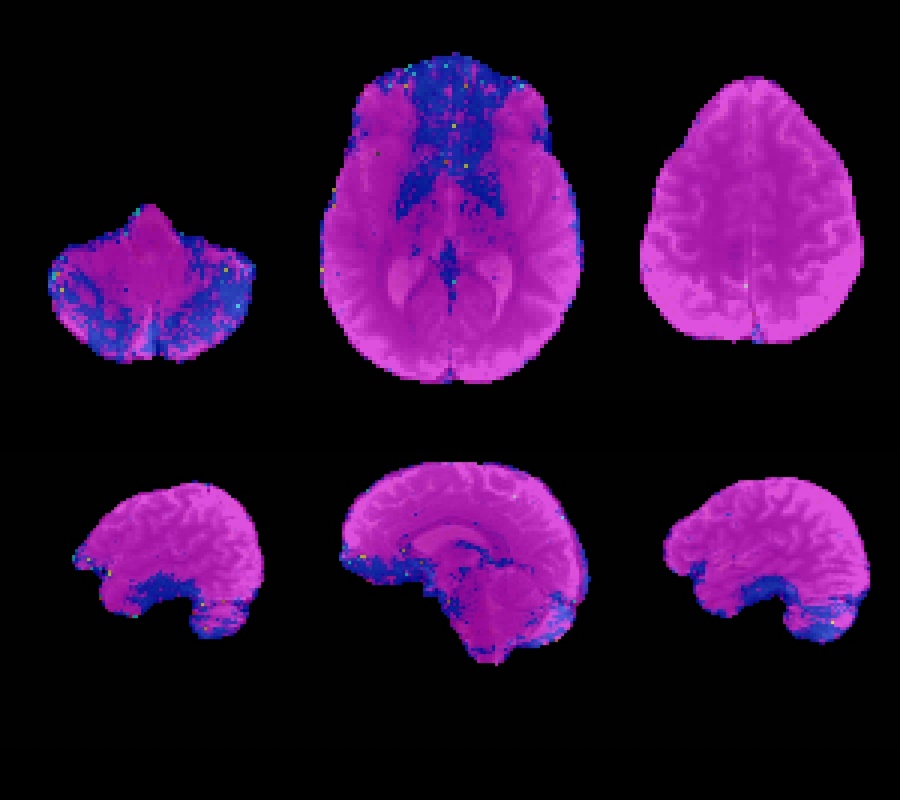
\includegraphics[width=3cm]{images/sub-001_ses-1_task-HABLA1700_S0meanSPC_part-mag_bold_tmppca_all} &\textcolor{white}{$\Delta S_0$} 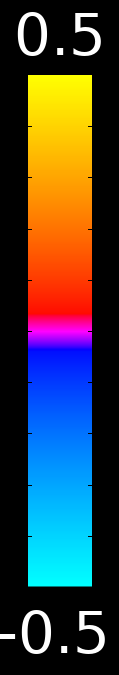
\includegraphics[width=.5cm]{images/SPC.png}\\
    \end{tabular}
    }
    \caption[$S_0^$  maps at low resolution (2 mm isotropic)]{Left: $S_0$ maps (2 mm). Right: $\Delta S_0$ (change relative to vanilla).}
    \label{fig:S01700}
\end{figure}

\begin{figure}[htbp]
\centering \colorbox{black}{
    \centering
    \begin{tabular}{>{\centering\arraybackslash}m{.7cm}>{\centering\arraybackslash}m{3cm}>{\centering\arraybackslash}m{3cm}>{\centering\arraybackslash}m{.7cm}}
    
       & \textcolor{white}{\textbf{$S_0$}} & \textcolor{white}{\textbf{$\Delta S_0$}}& \\
   \rotatebox[origin=l]{90}{\textcolor{white}{VANILLA}}
  &    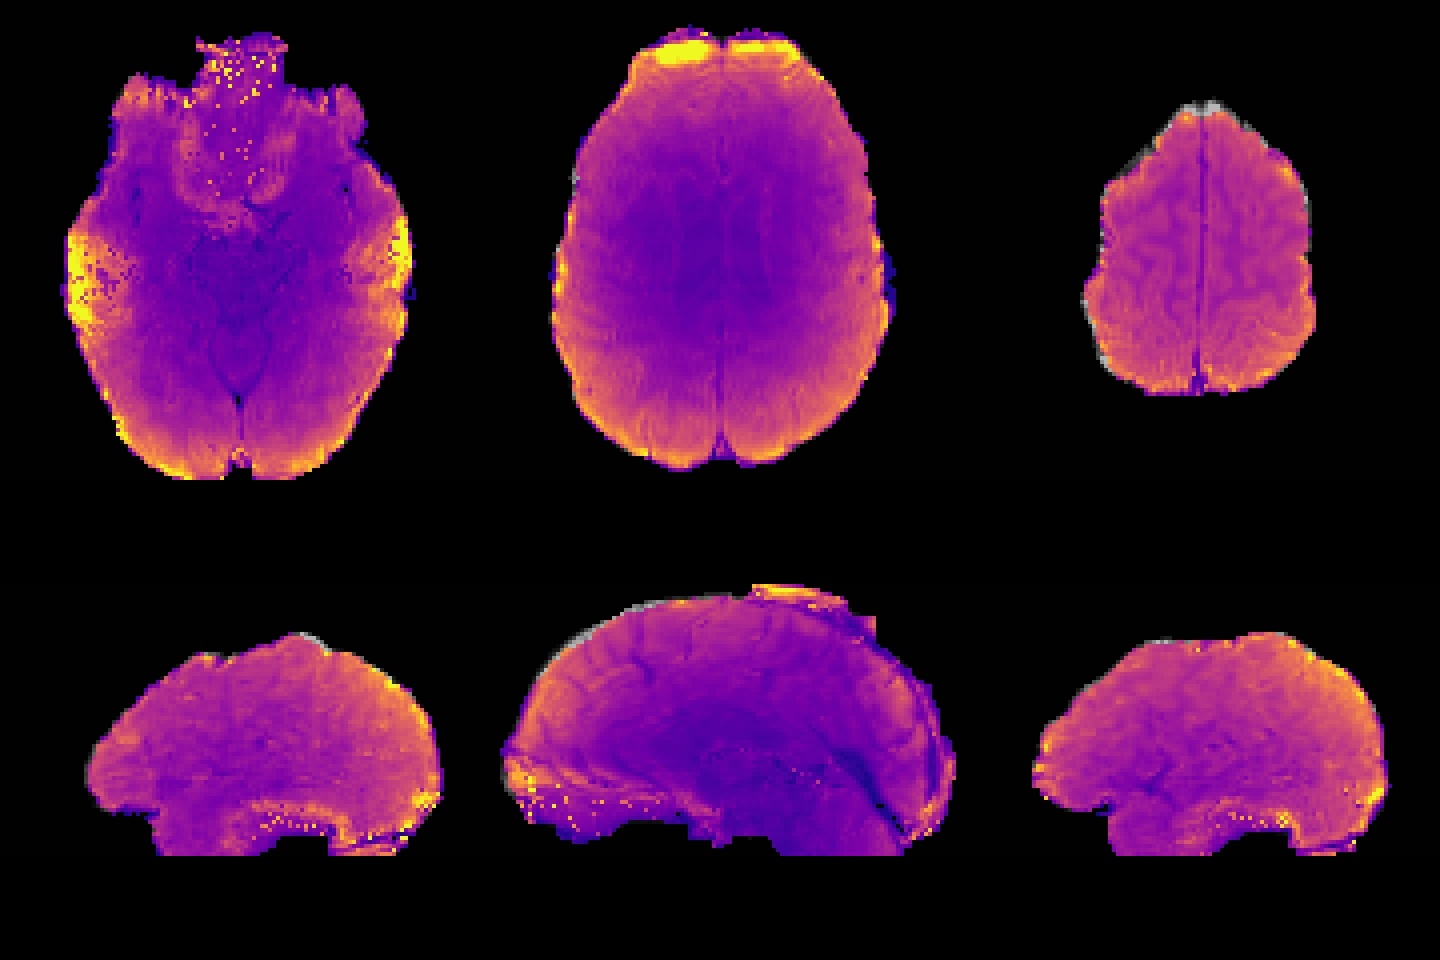
\includegraphics[width=3cm]{images/sub-001_ses-1_task-REST_run-1_S0mean_part-mag_bold_vanilla_all.jpg} & & \textcolor{white}{$S_0$} 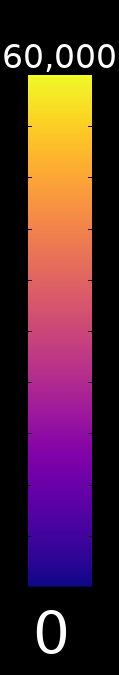
\includegraphics[width=.5cm]{images/Plasmas0.png}\\
     \rotatebox[origin=l]{90}{\textcolor{white}{MPPCA}}
  &    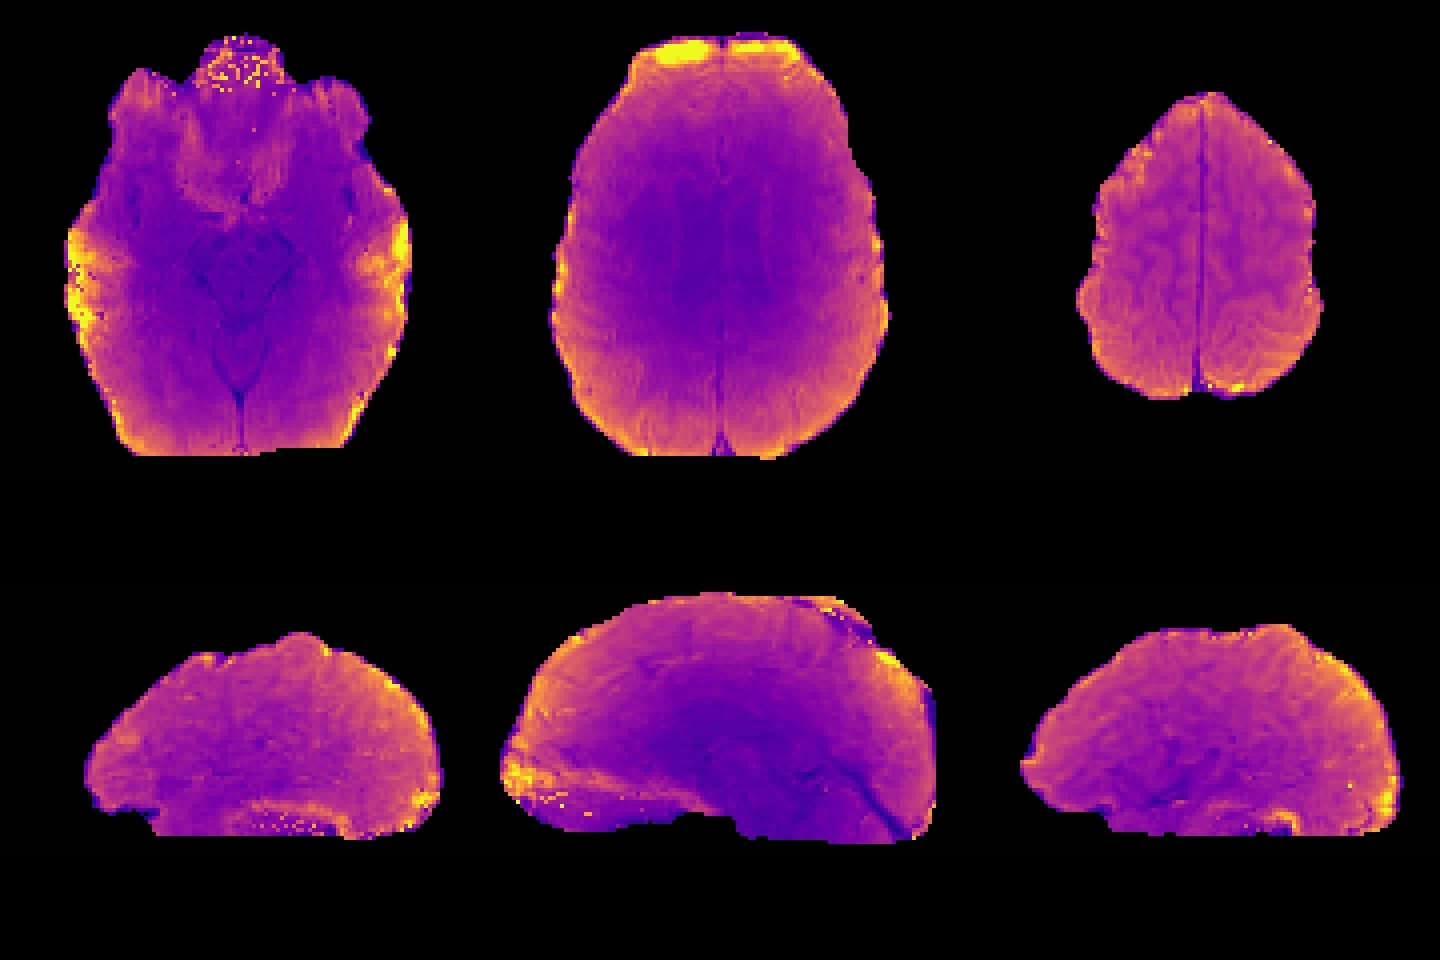
\includegraphics[width=3cm]{images/sub-001_ses-1_task-REST_run-1_S0mean_part-mag_bold_mppca_all} &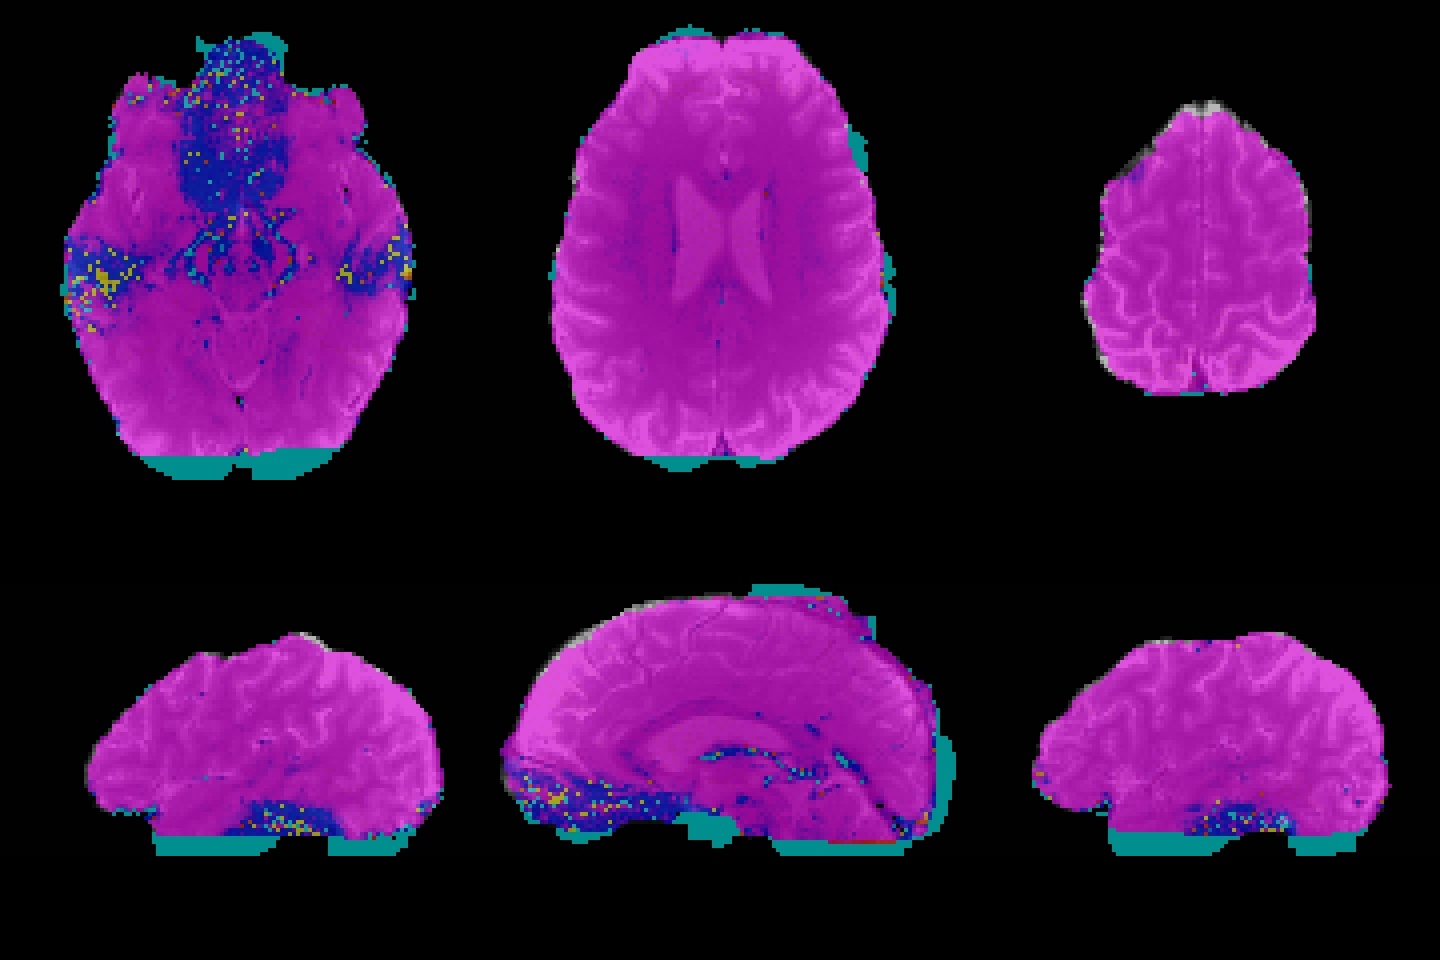
\includegraphics[width=3cm]{images/sub-001_ses-1_task-REST_run-1_S0meanSPC_part-mag_bold_mppca_all} &\\
       \rotatebox[origin=l]{90}{\textcolor{white}{NORDIC}}
  &    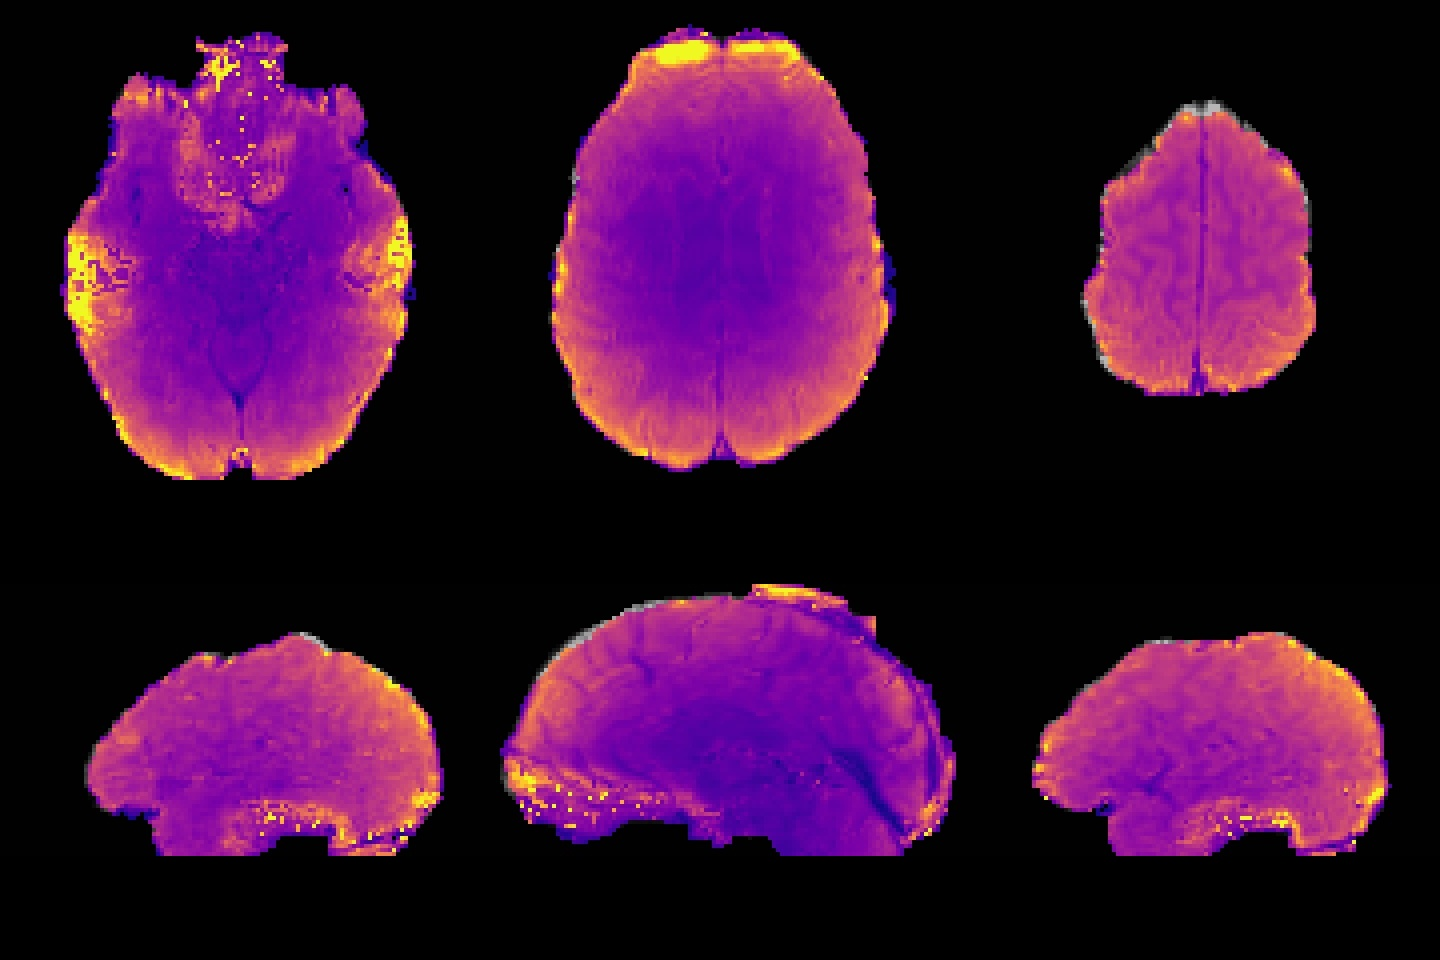
\includegraphics[width=3cm]{images/sub-001_ses-1_task-REST_run-1_S0mean_part-mag_bold_nordic_all.jpg} &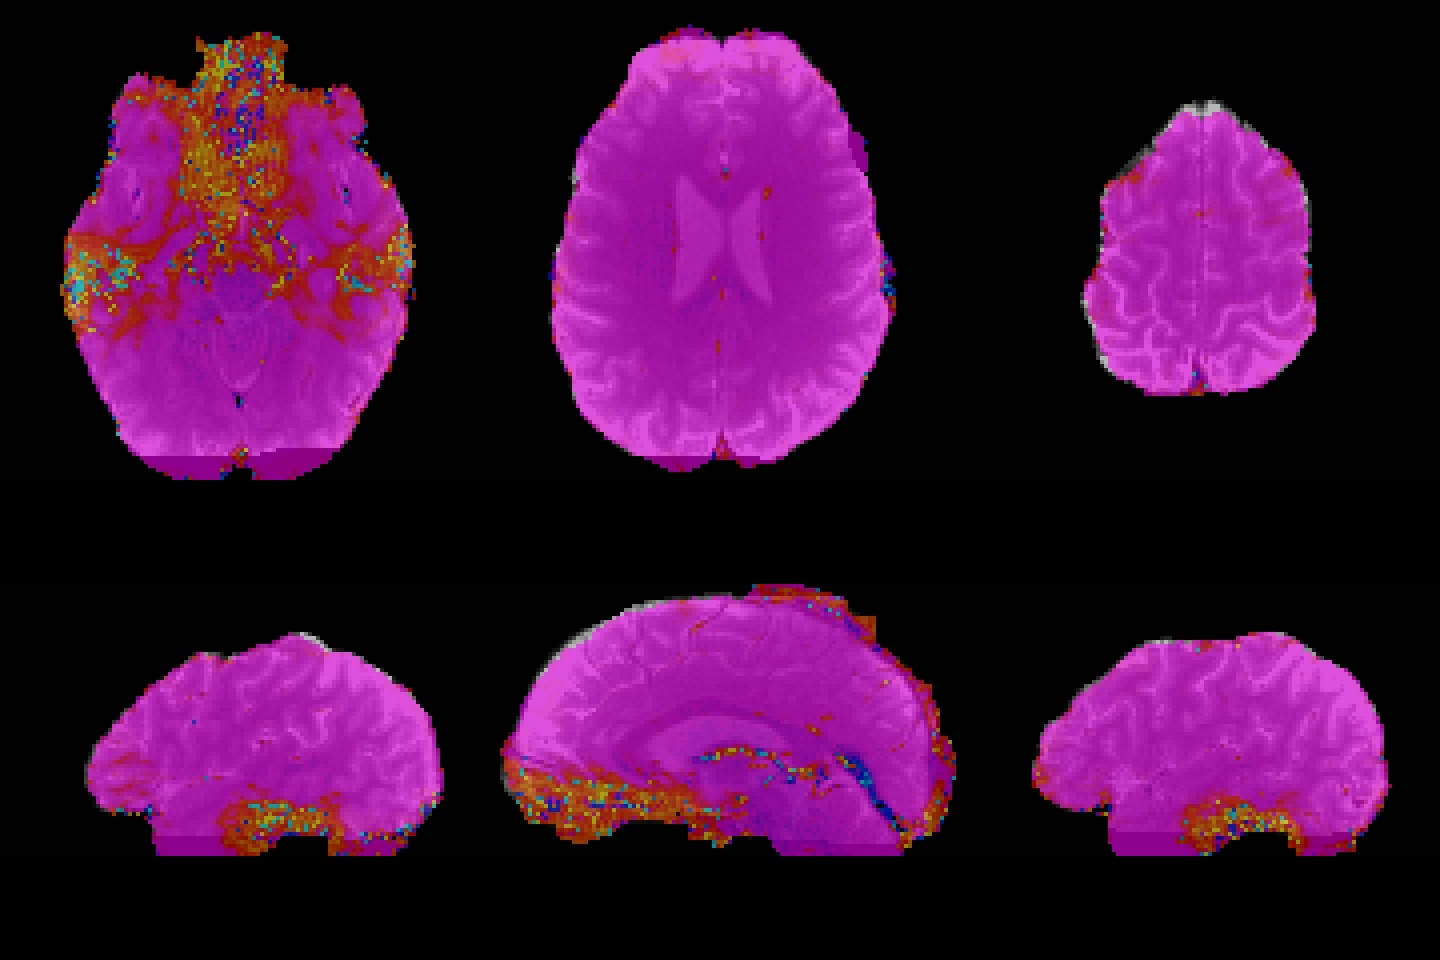
\includegraphics[width=3cm]{images/sub-001_ses-1_task-REST_run-1_S0meanSPC_part-mag_bold_nordic_all} &\\
       \rotatebox[origin=l]{90}{\textcolor{white}{HYDRA}}
  &    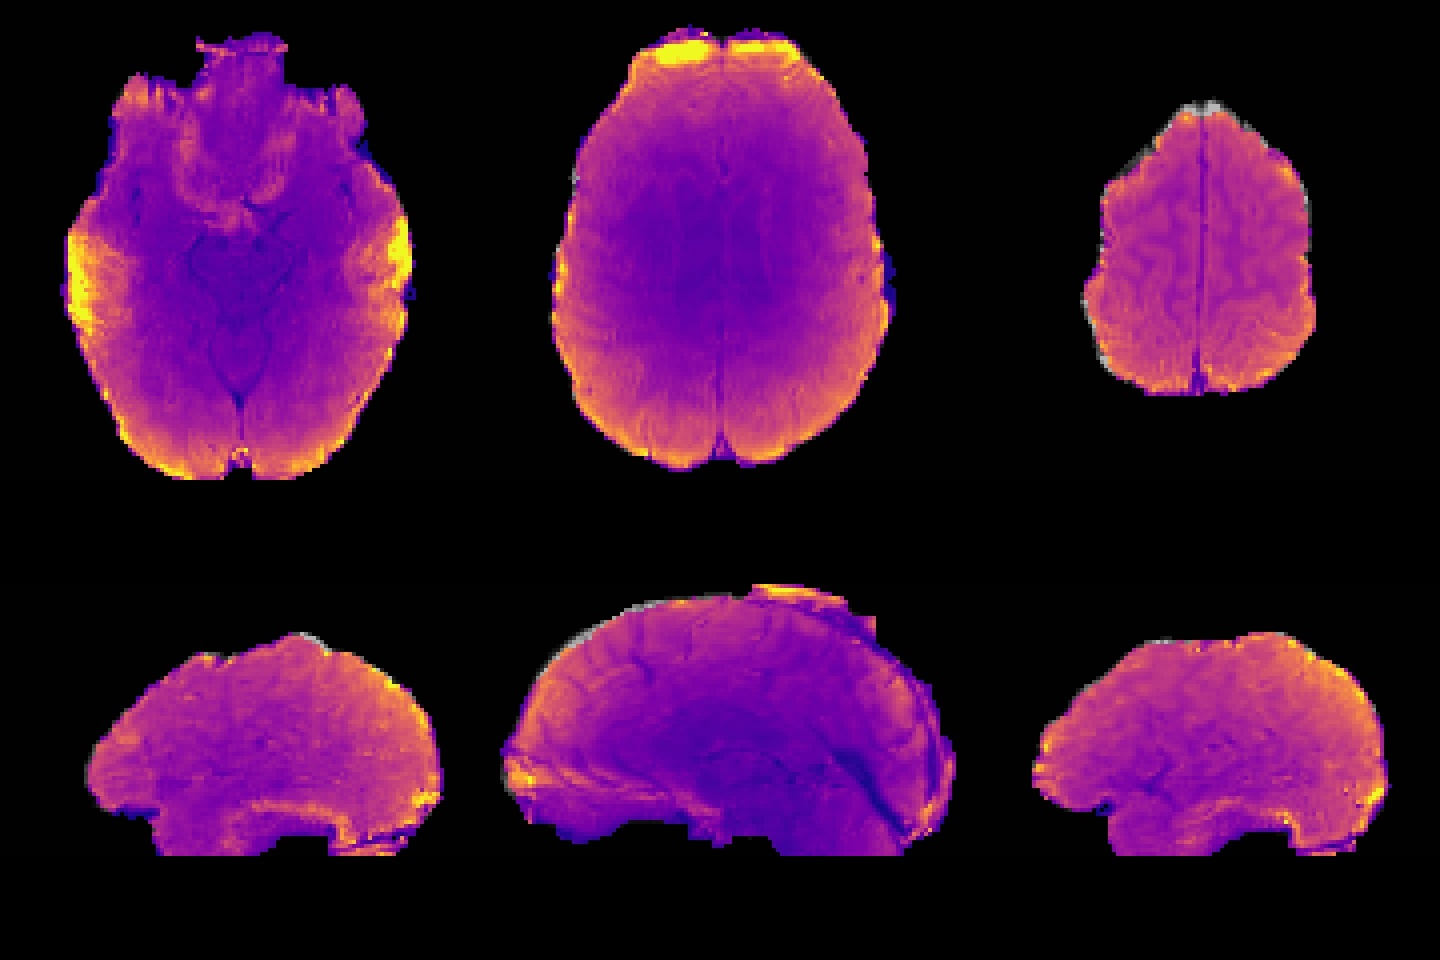
\includegraphics[width=3cm]{images/sub-001_ses-1_task-REST_run-1_S0mean_part-mag_bold_hydra_all.jpg} &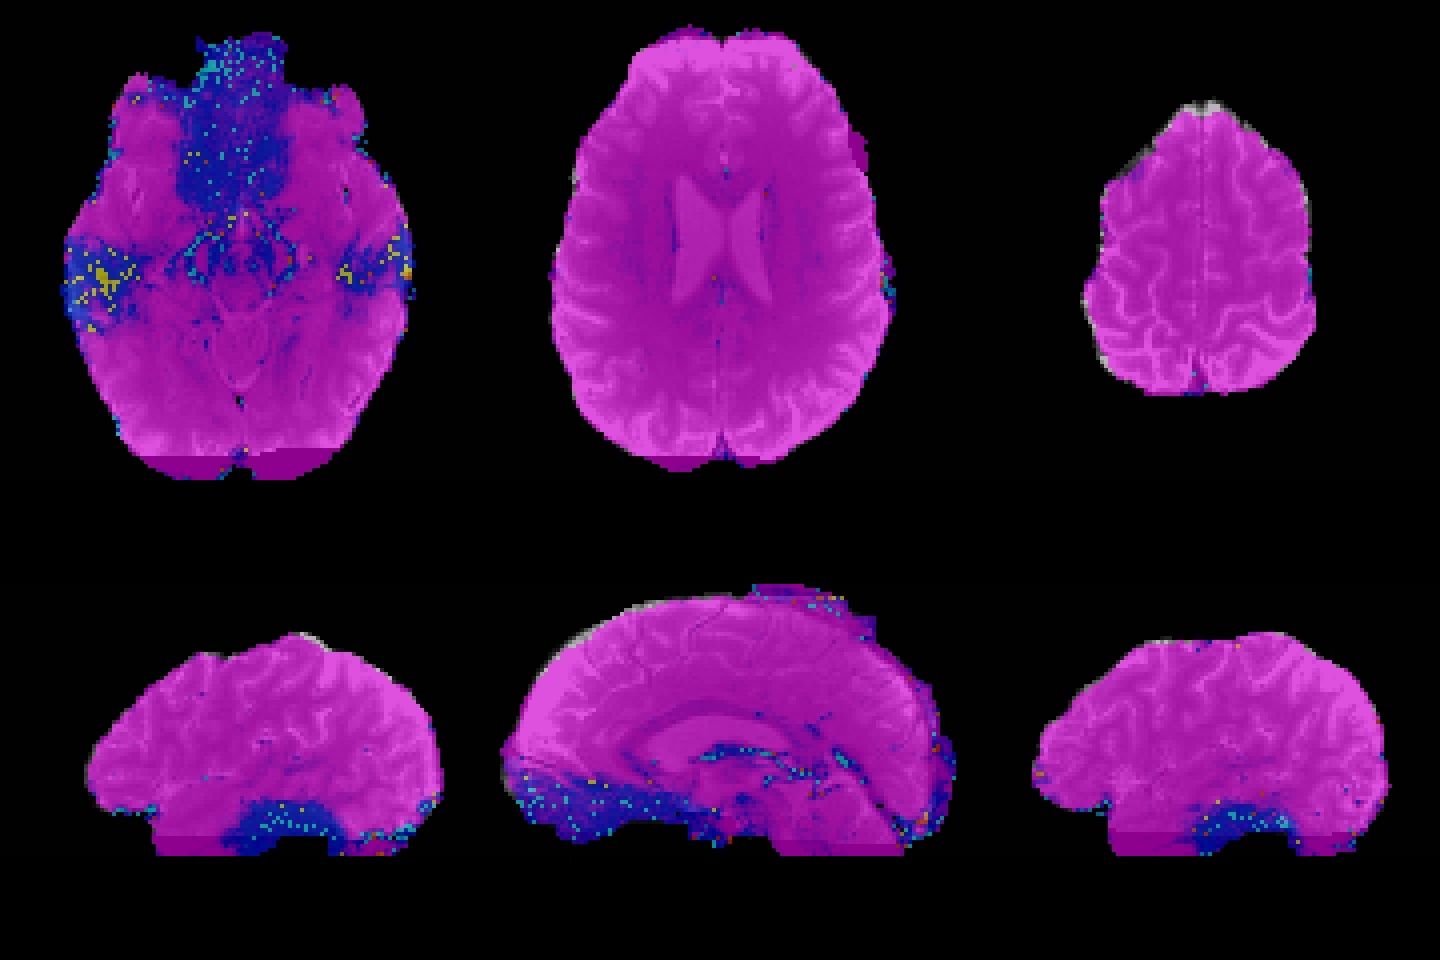
\includegraphics[width=3cm]{images/sub-001_ses-1_task-REST_run-1_S0meanSPC_part-mag_bold_hydra_all} &\\
       \rotatebox[origin=l]{90}{\textcolor{white}{TMPPCA}}
  &    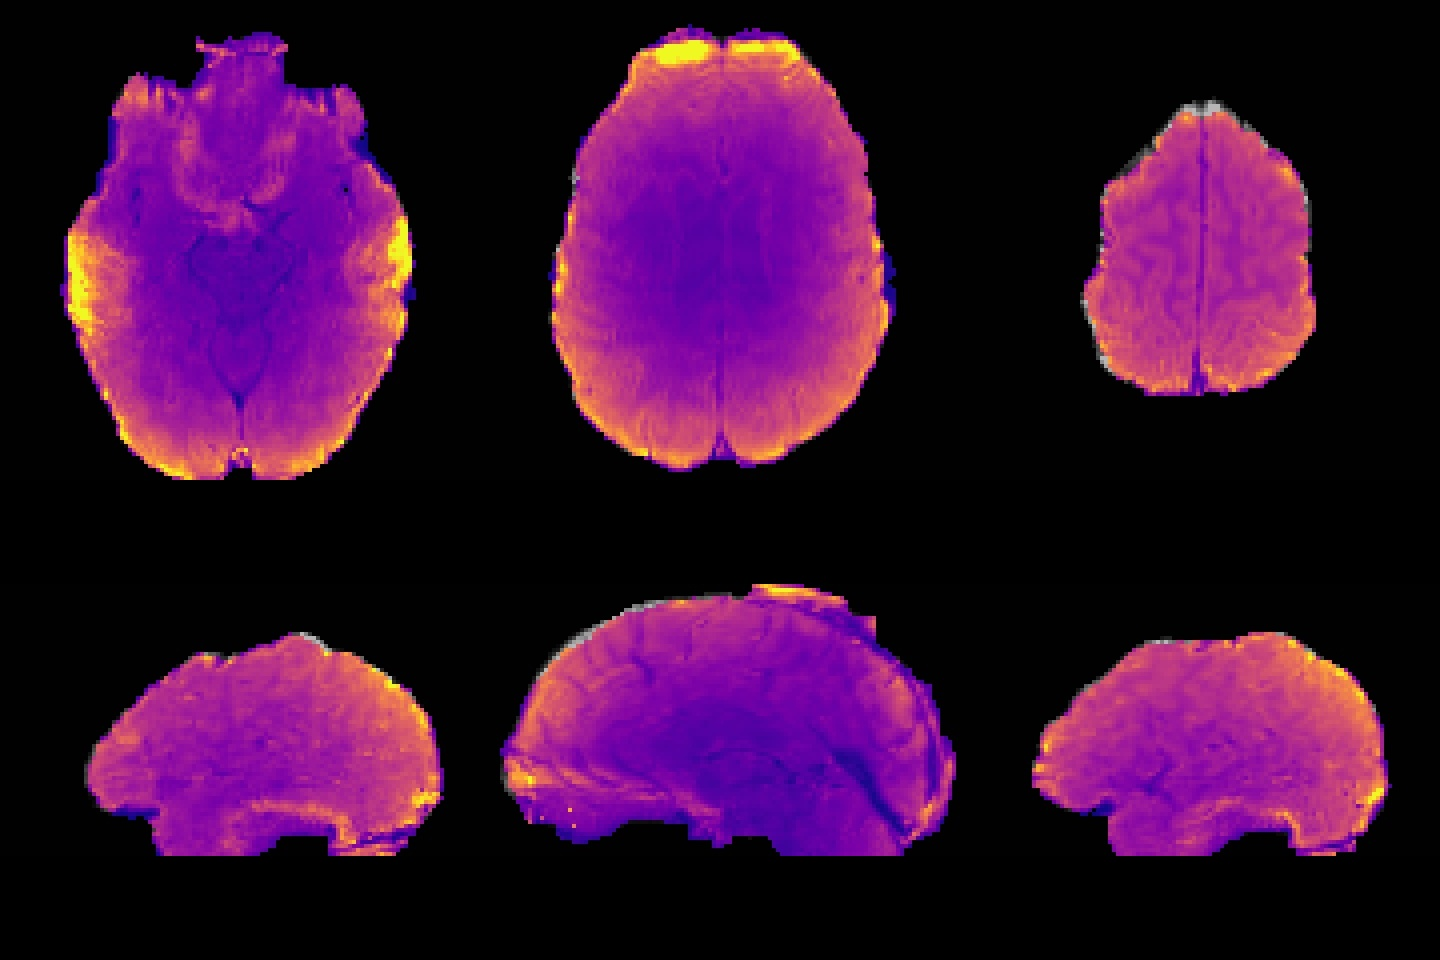
\includegraphics[width=3cm]{images/sub-001_ses-1_task-REST_run-1_S0mean_part-mag_bold_tmppca_all.jpg} &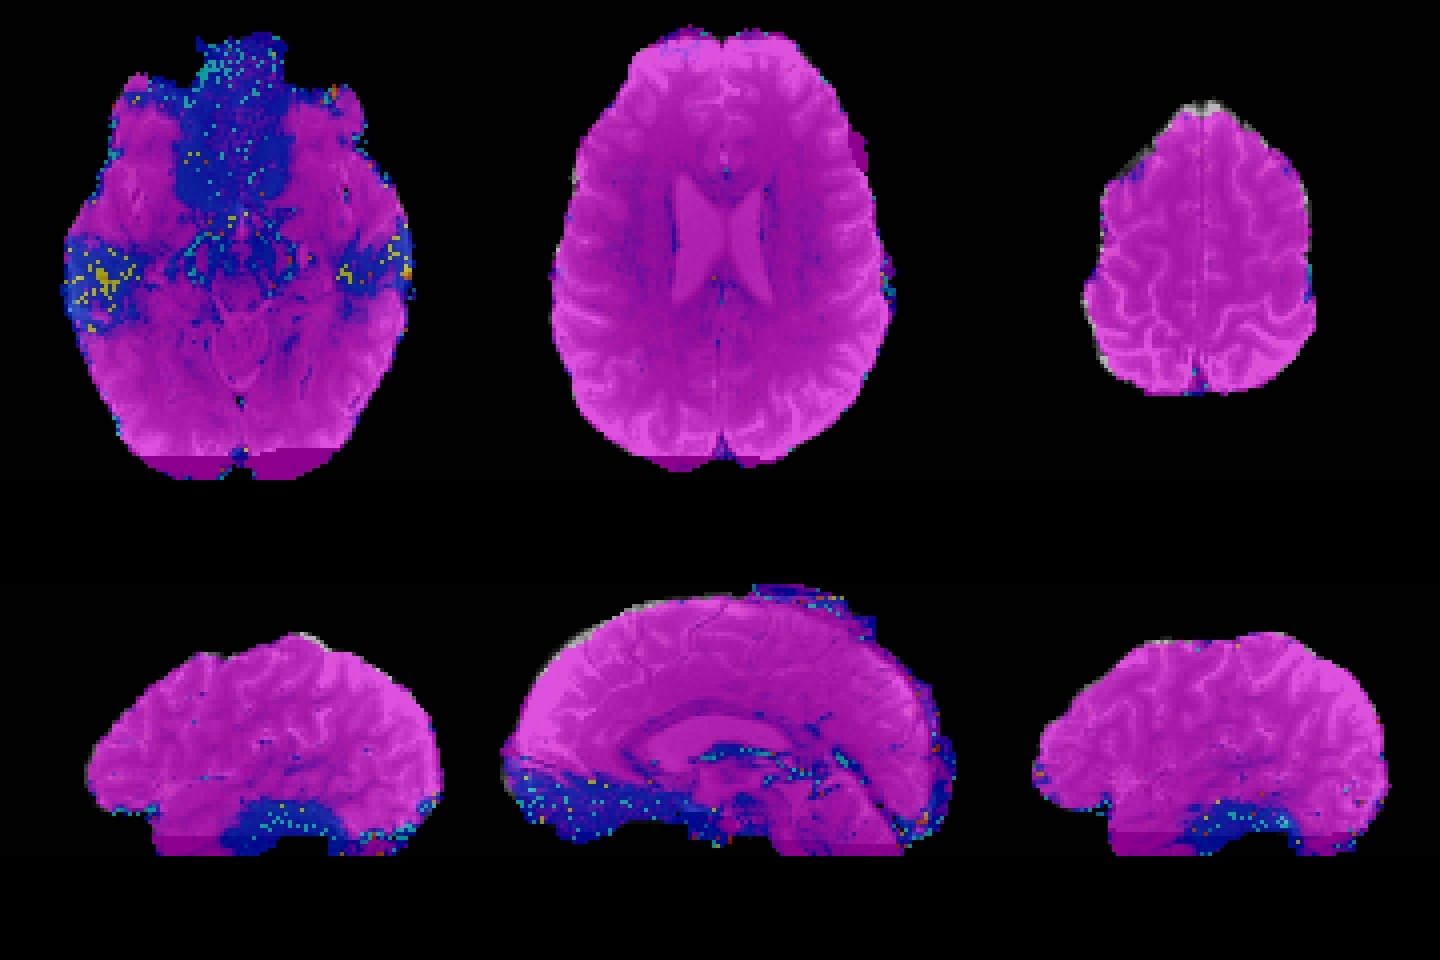
\includegraphics[width=3cm]{images/sub-001_ses-1_task-REST_run-1_S0meanSPC_part-mag_bold_tmppca_all} &\textcolor{white}{$\Delta S_0$} 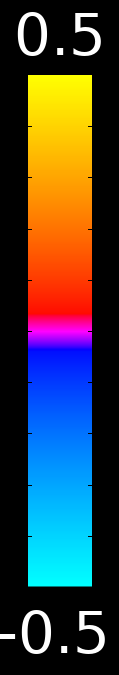
\includegraphics[width=.5cm]{images/SPC.png}\\
    \end{tabular}
    }
    \caption[$S_0^$  maps at high resolution (1.5 mm isotropic)]{Left: $S_0$ maps (1.5 mm). Right: $\Delta S_0$ (change relative to vanilla).}
    \label{fig:S0hr}
\end{figure}

%-- boxplot

\begin{figure}[htbp]
\centering \colorbox{white}{
    \centering
    \begin{tabular}{>{\centering\arraybackslash}m{.7cm}>{\centering\arraybackslash}m{7cm}}
       & \textcolor{black}{\textbf{$S0$}} \\
    \rotatebox[origin=l]{90}{\textcolor{black}{2.4 mm}} &    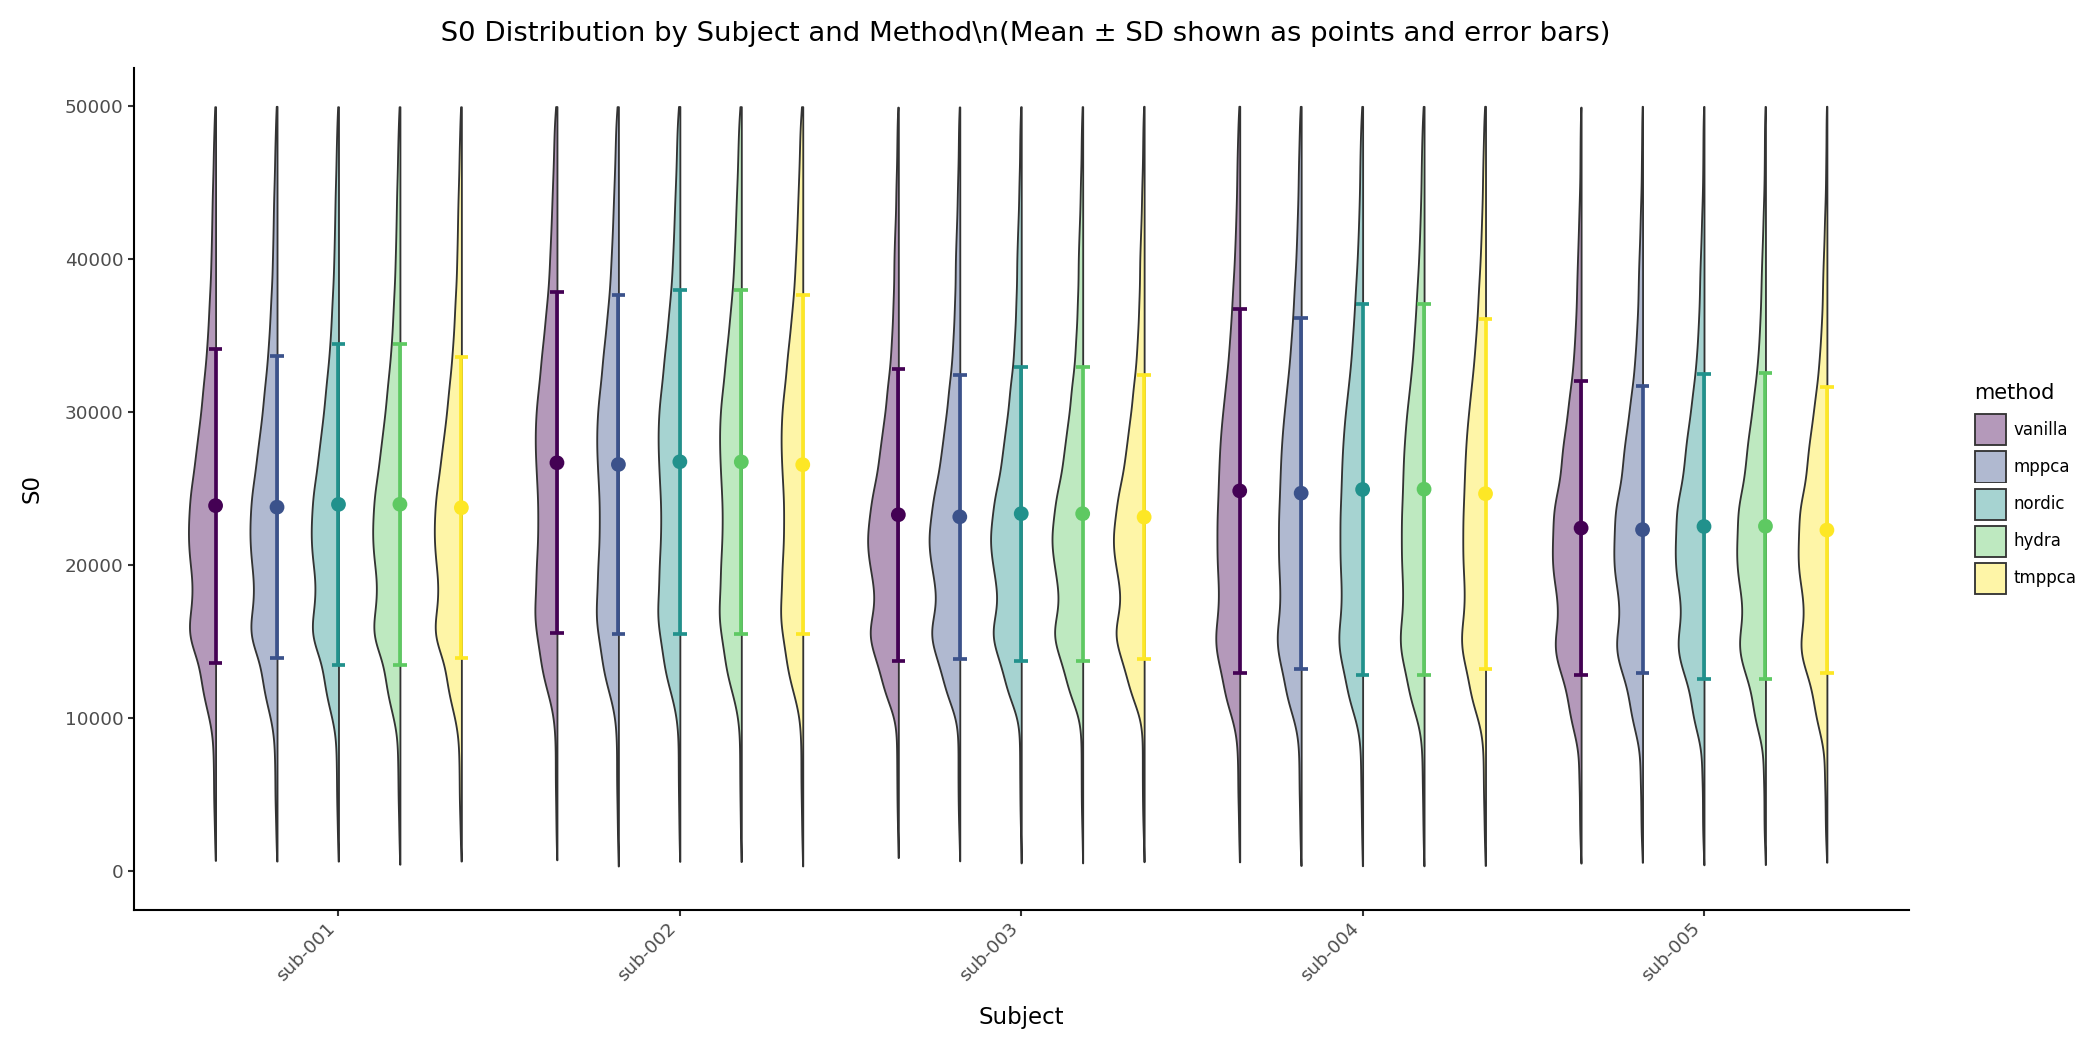
\includegraphics[width=7cm]{images/halfviolin_s0_across_subjects_masked1200.png}\\
       \rotatebox[origin=l]{90}{\textcolor{black}{2 mm}} & 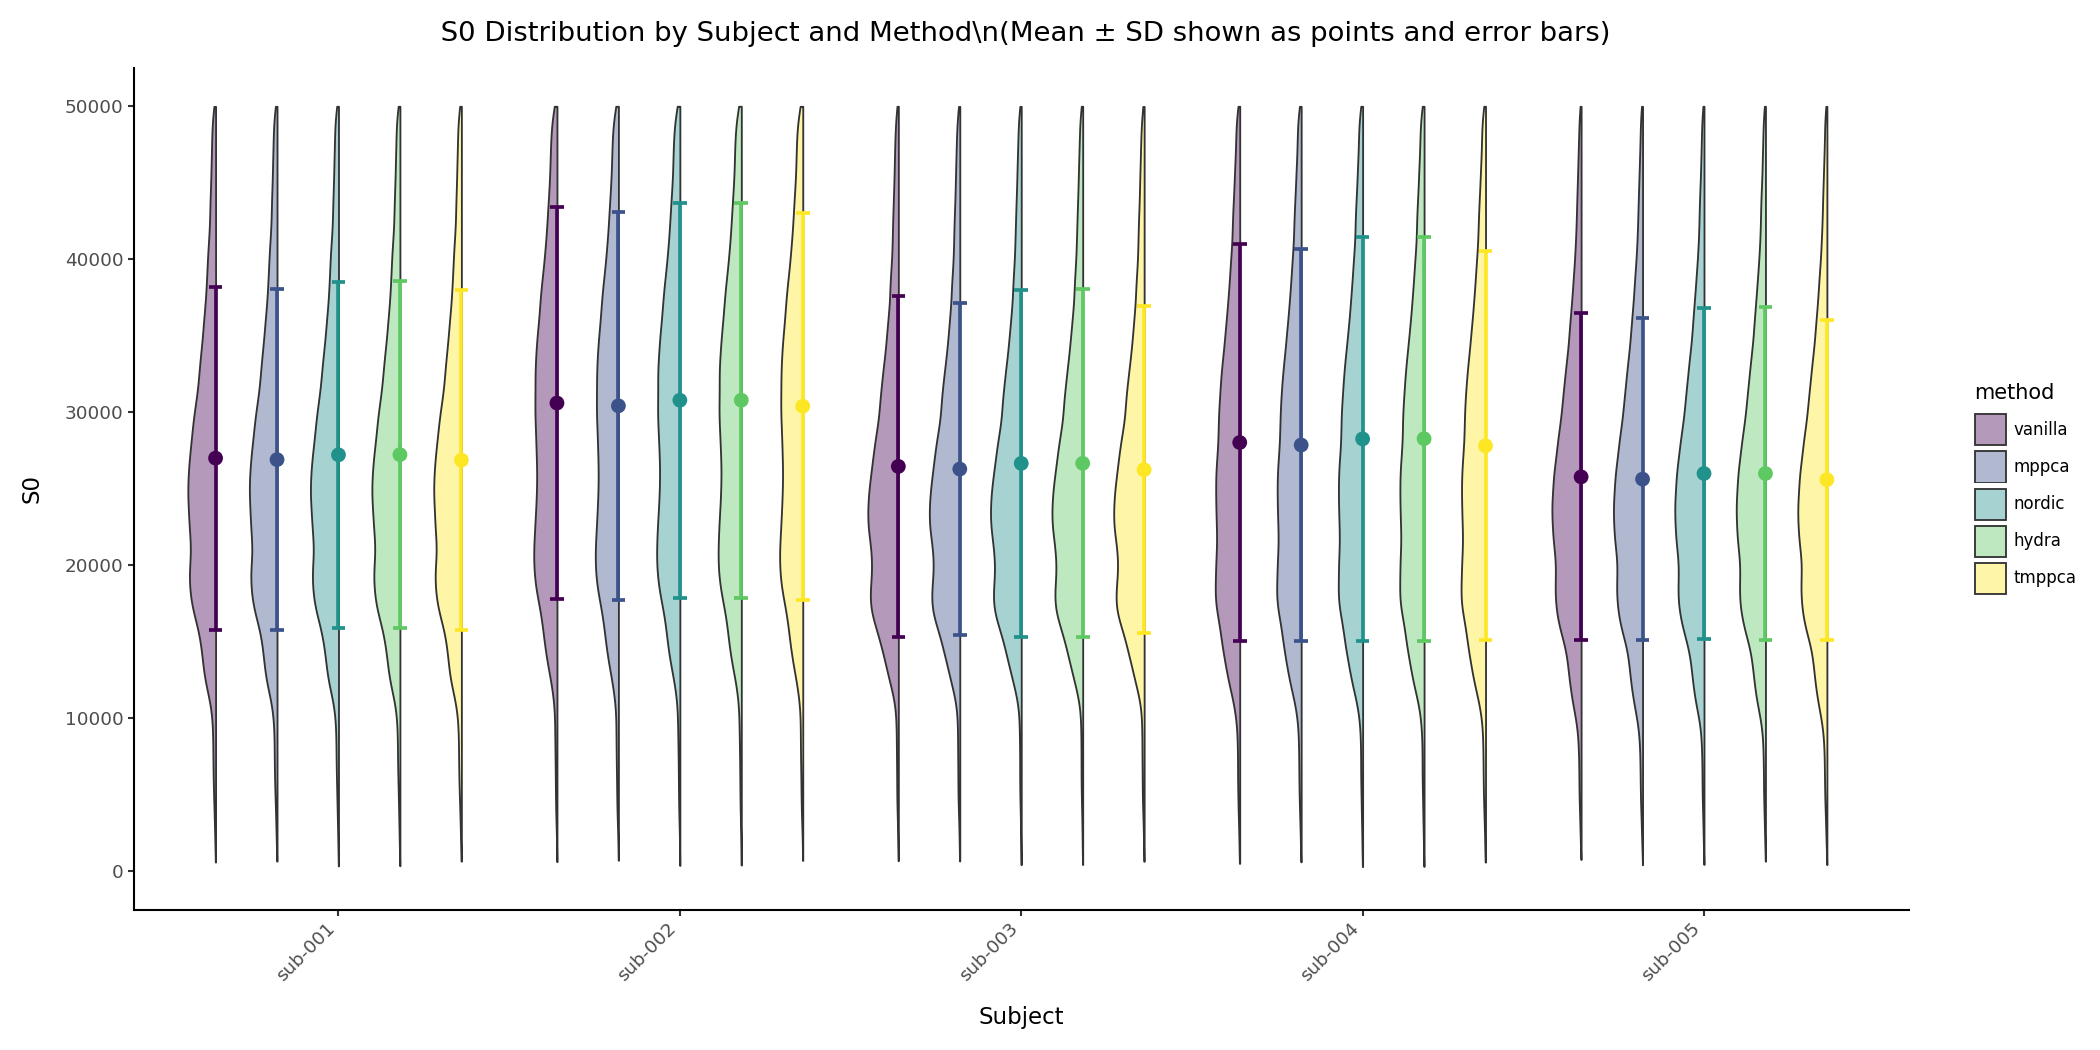
\includegraphics[width=7cm]{images/halfviolin_s0_across_subjects_masked1700.png}\\
      \rotatebox[origin=l]{90}{\textcolor{black}{1.5 mm}}&   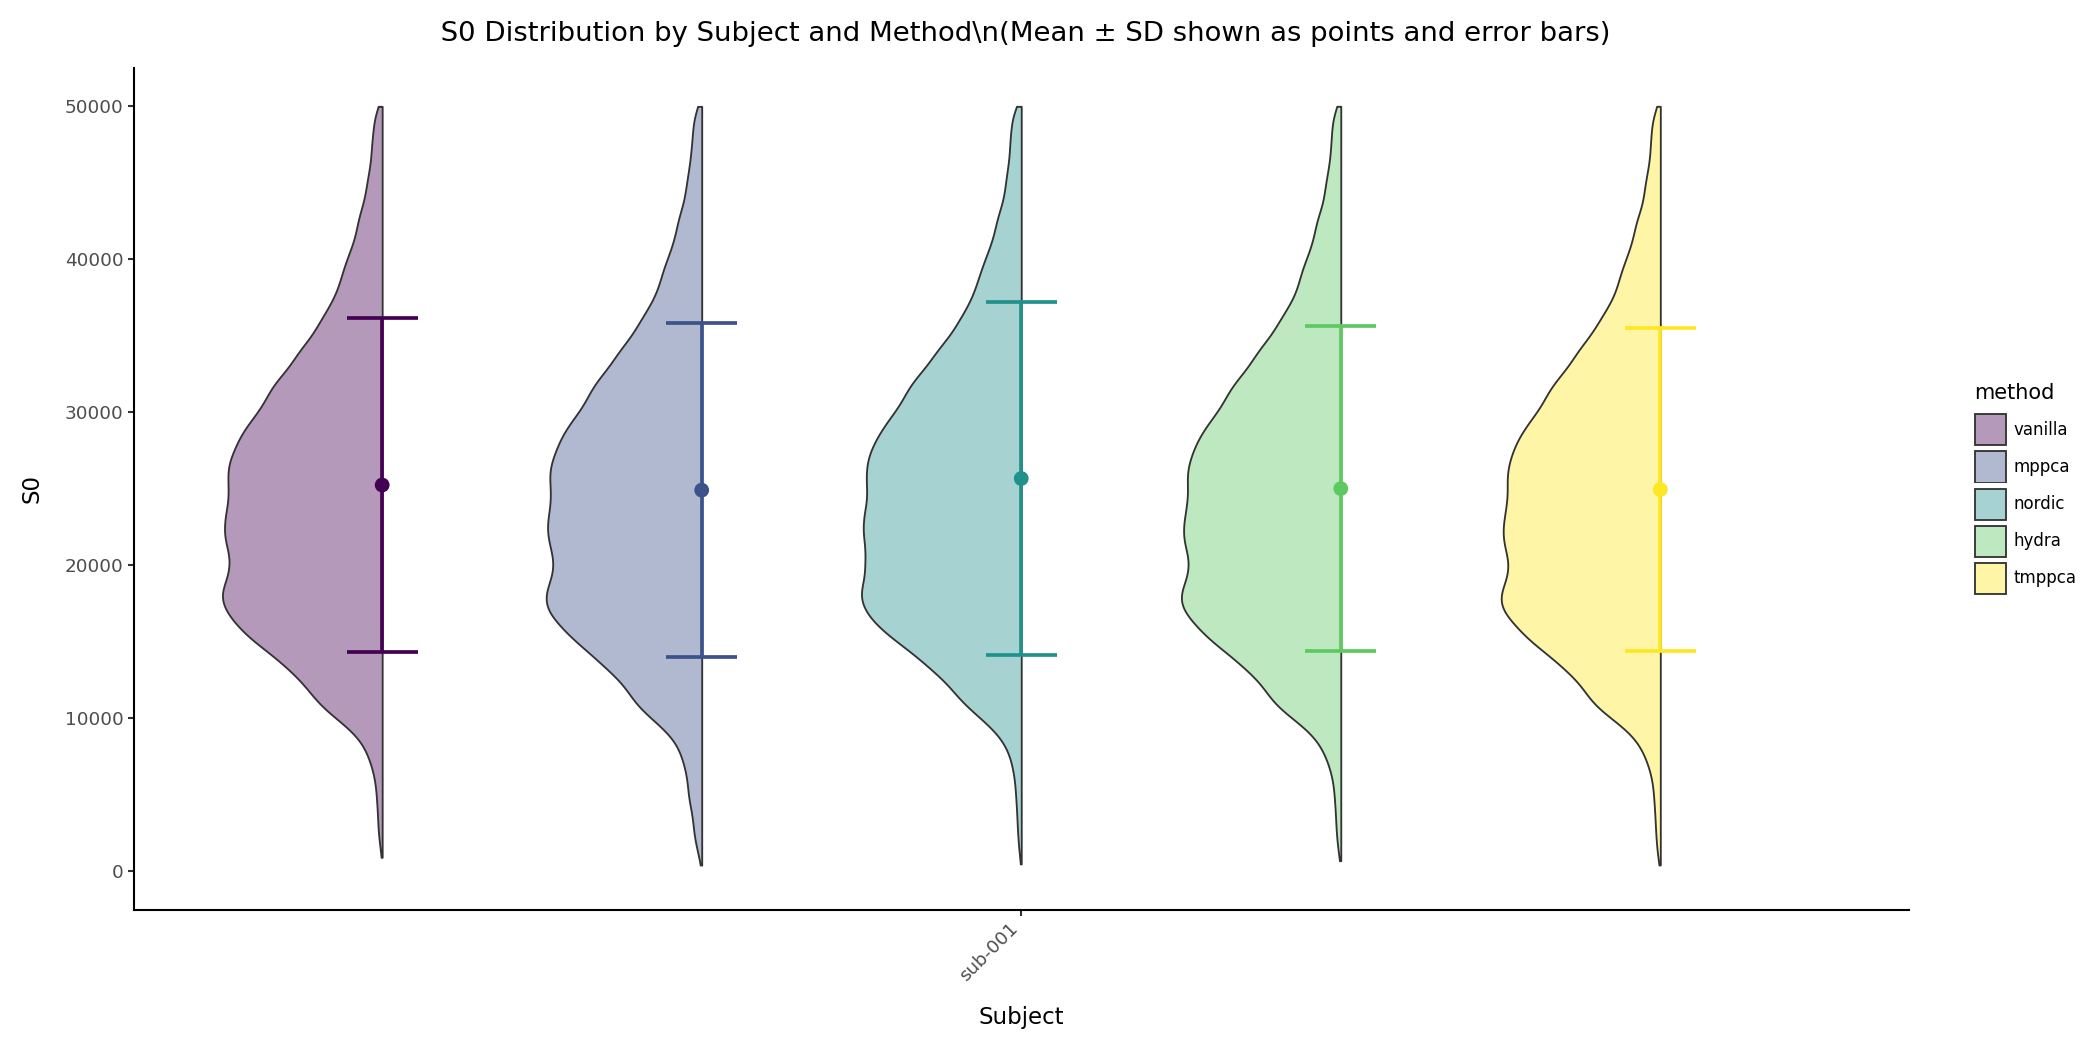
\includegraphics[width=7cm]{images/halfviolin_s0_across_subjects_maskedHR.png}
    \end{tabular}
    }
    \centering
    \caption[Distribution of $S0$ values per dataset]{ Histograms of $S_0$ values per dataset. }
    \label{fig:boxplotS0}
\end{figure}

\begin{figure}[htbp]
\centering \colorbox{white}{
    \centering
    \begin{tabular}{>{\centering\arraybackslash}m{.7cm}>{\centering\arraybackslash}m{7cm}}
        & \textcolor{black}{\textbf{$\Delta S_0$}} \\
    \rotatebox[origin=l]{90}{\textcolor{black}{2.4 mm}}&
        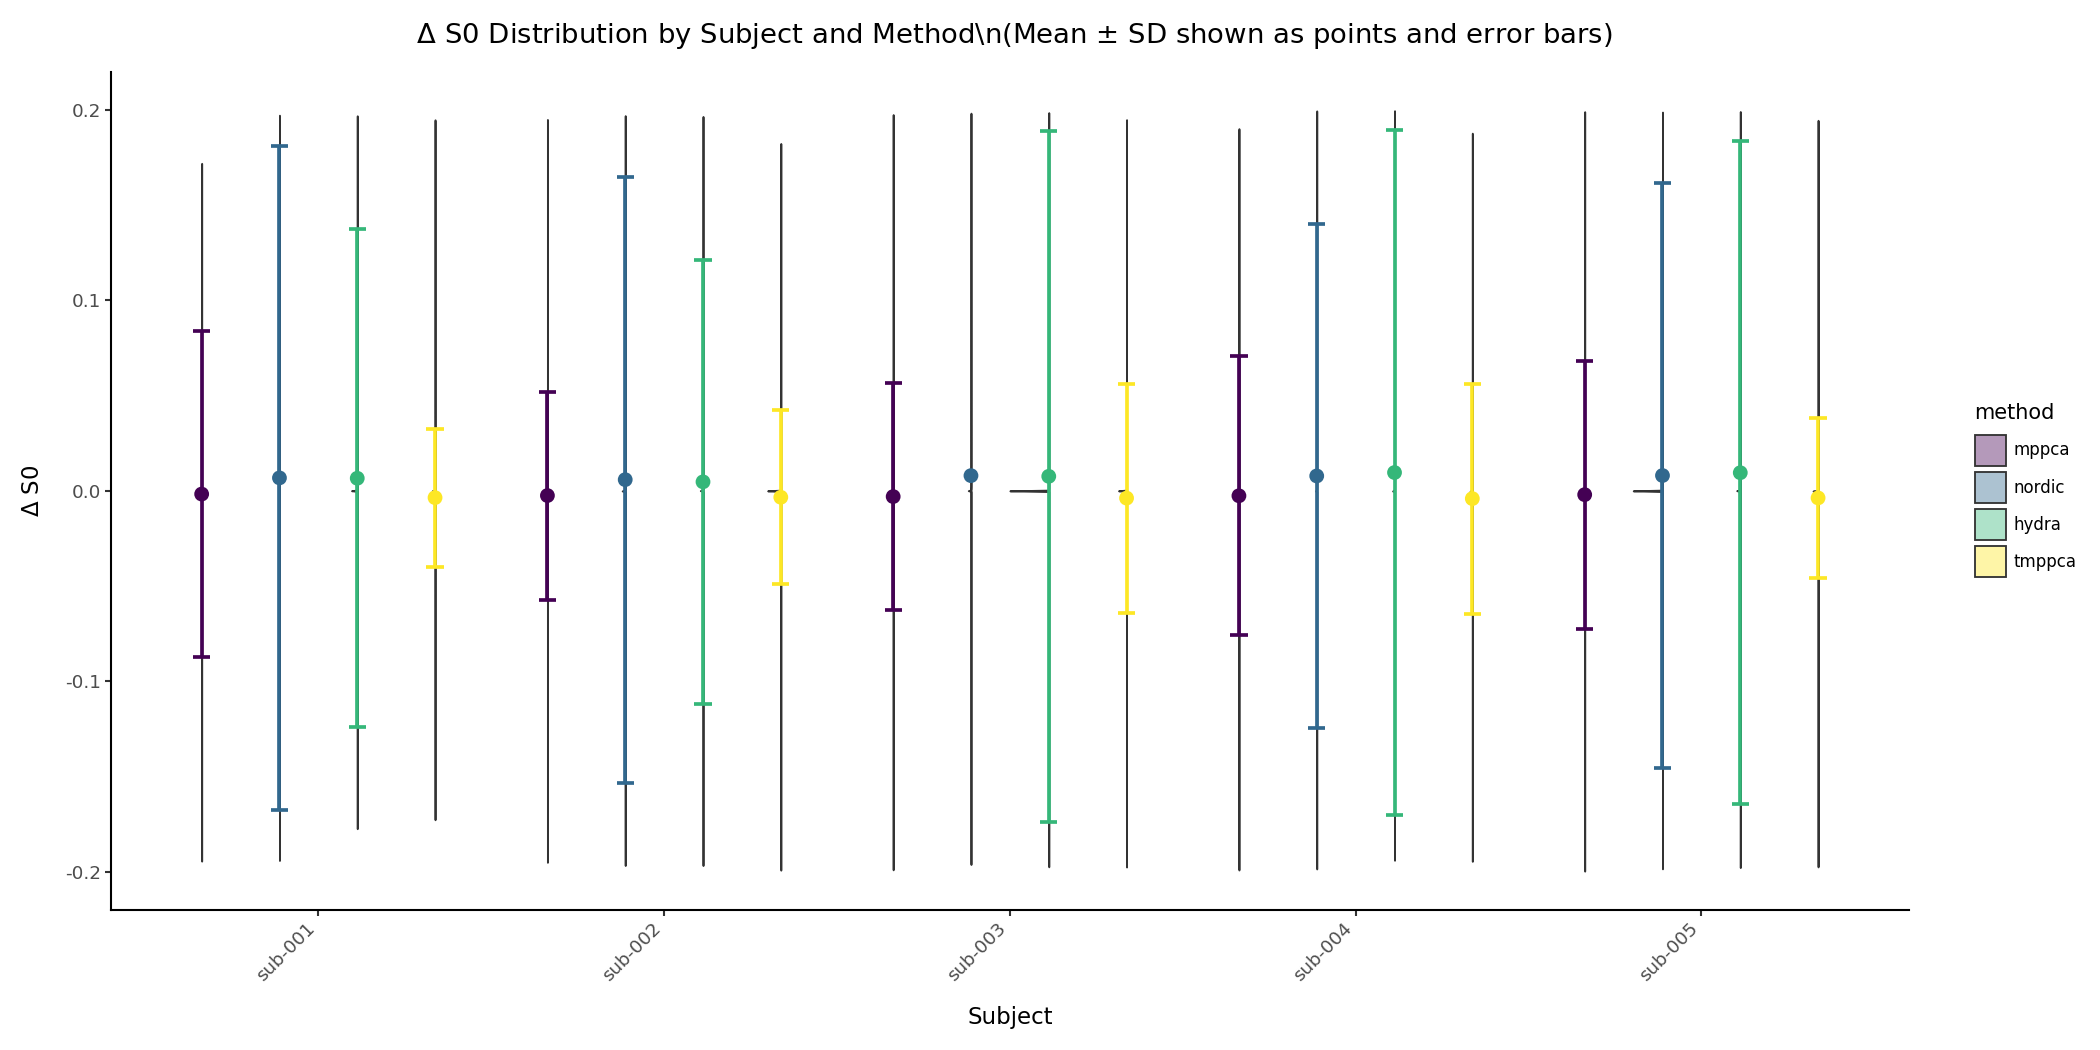
\includegraphics[width=7cm]{images/halfviolin_s0spc_across_subjects_masked1200.png}\\
       \rotatebox[origin=l]{90}{\textcolor{black}{2 mm}} &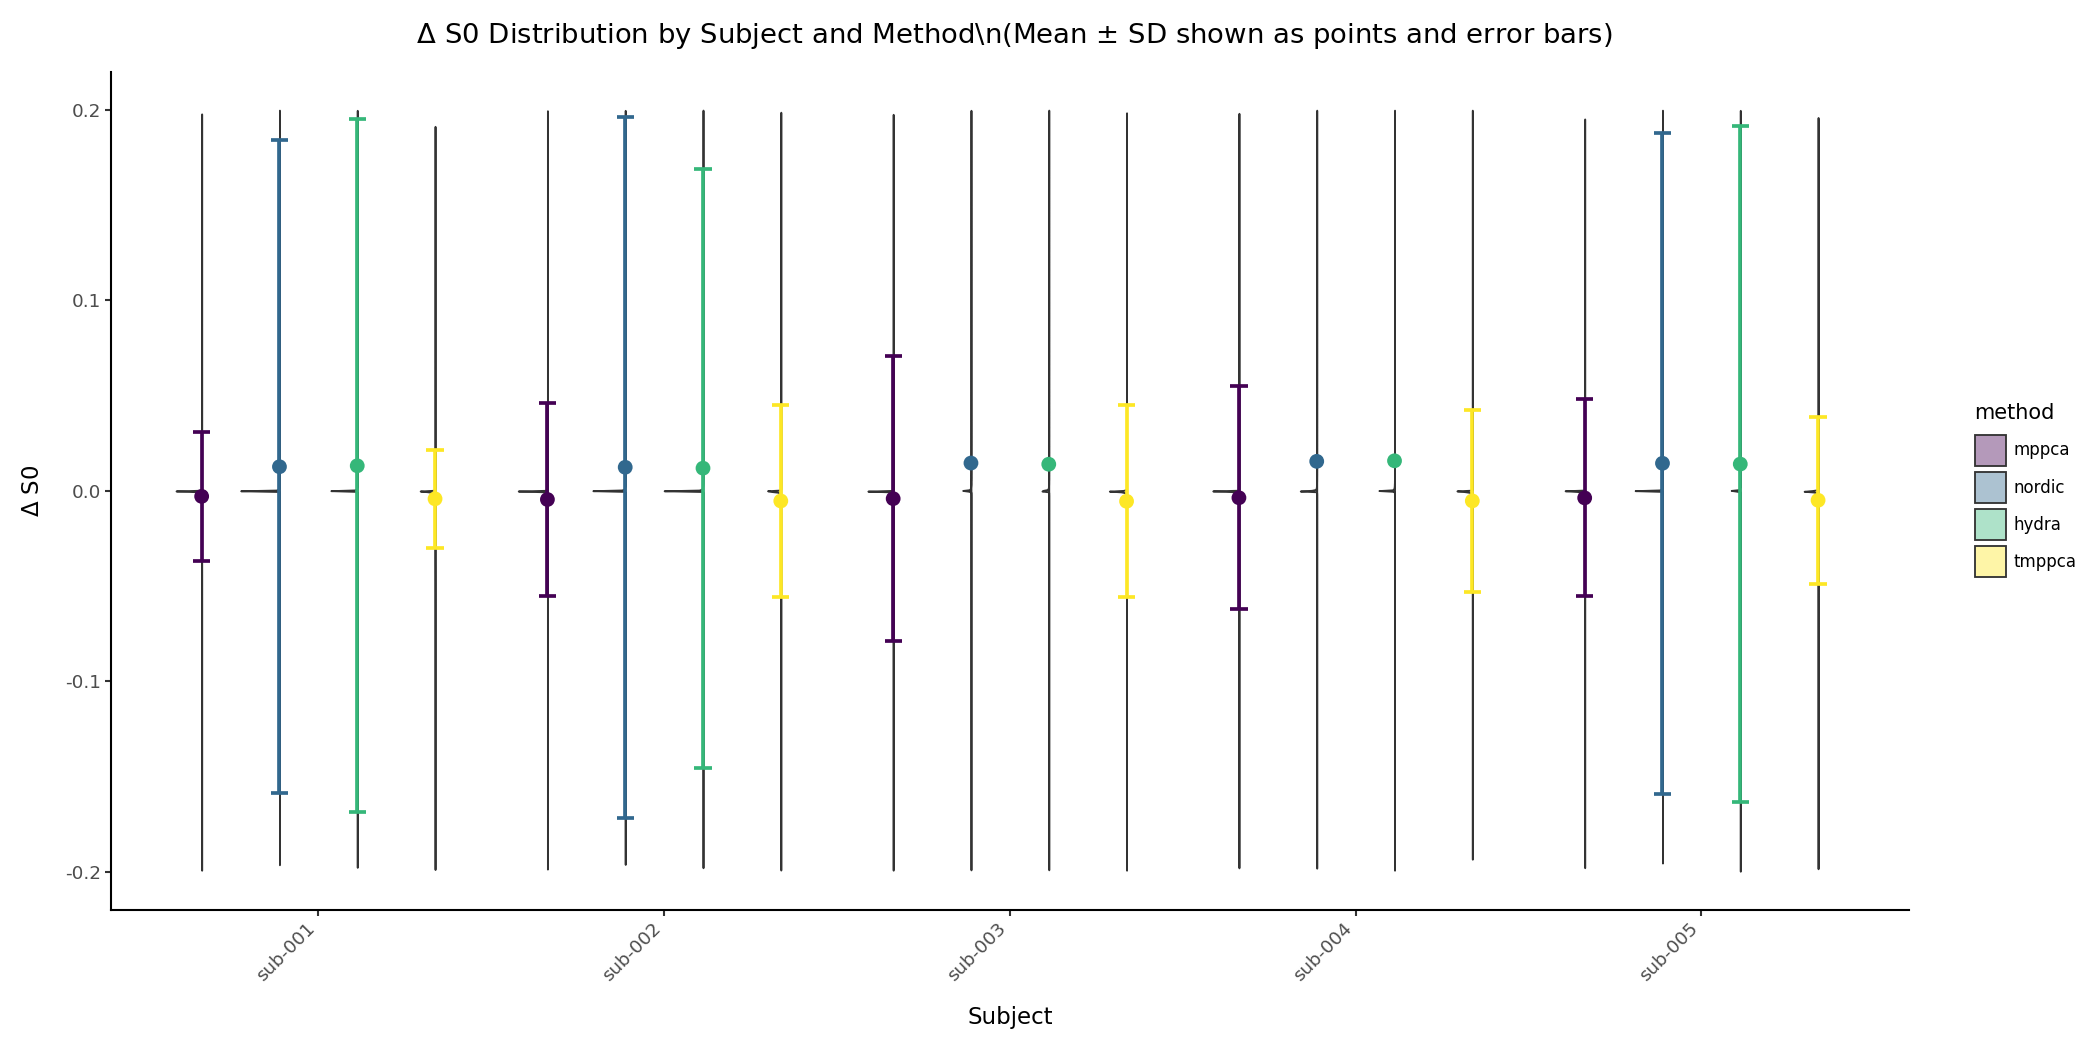
\includegraphics[width=7cm]{images/halfviolin_s0spc_across_subjects_masked1700.png} \\
      \rotatebox[origin=l]{90}{\textcolor{black}{1.5 mm}}&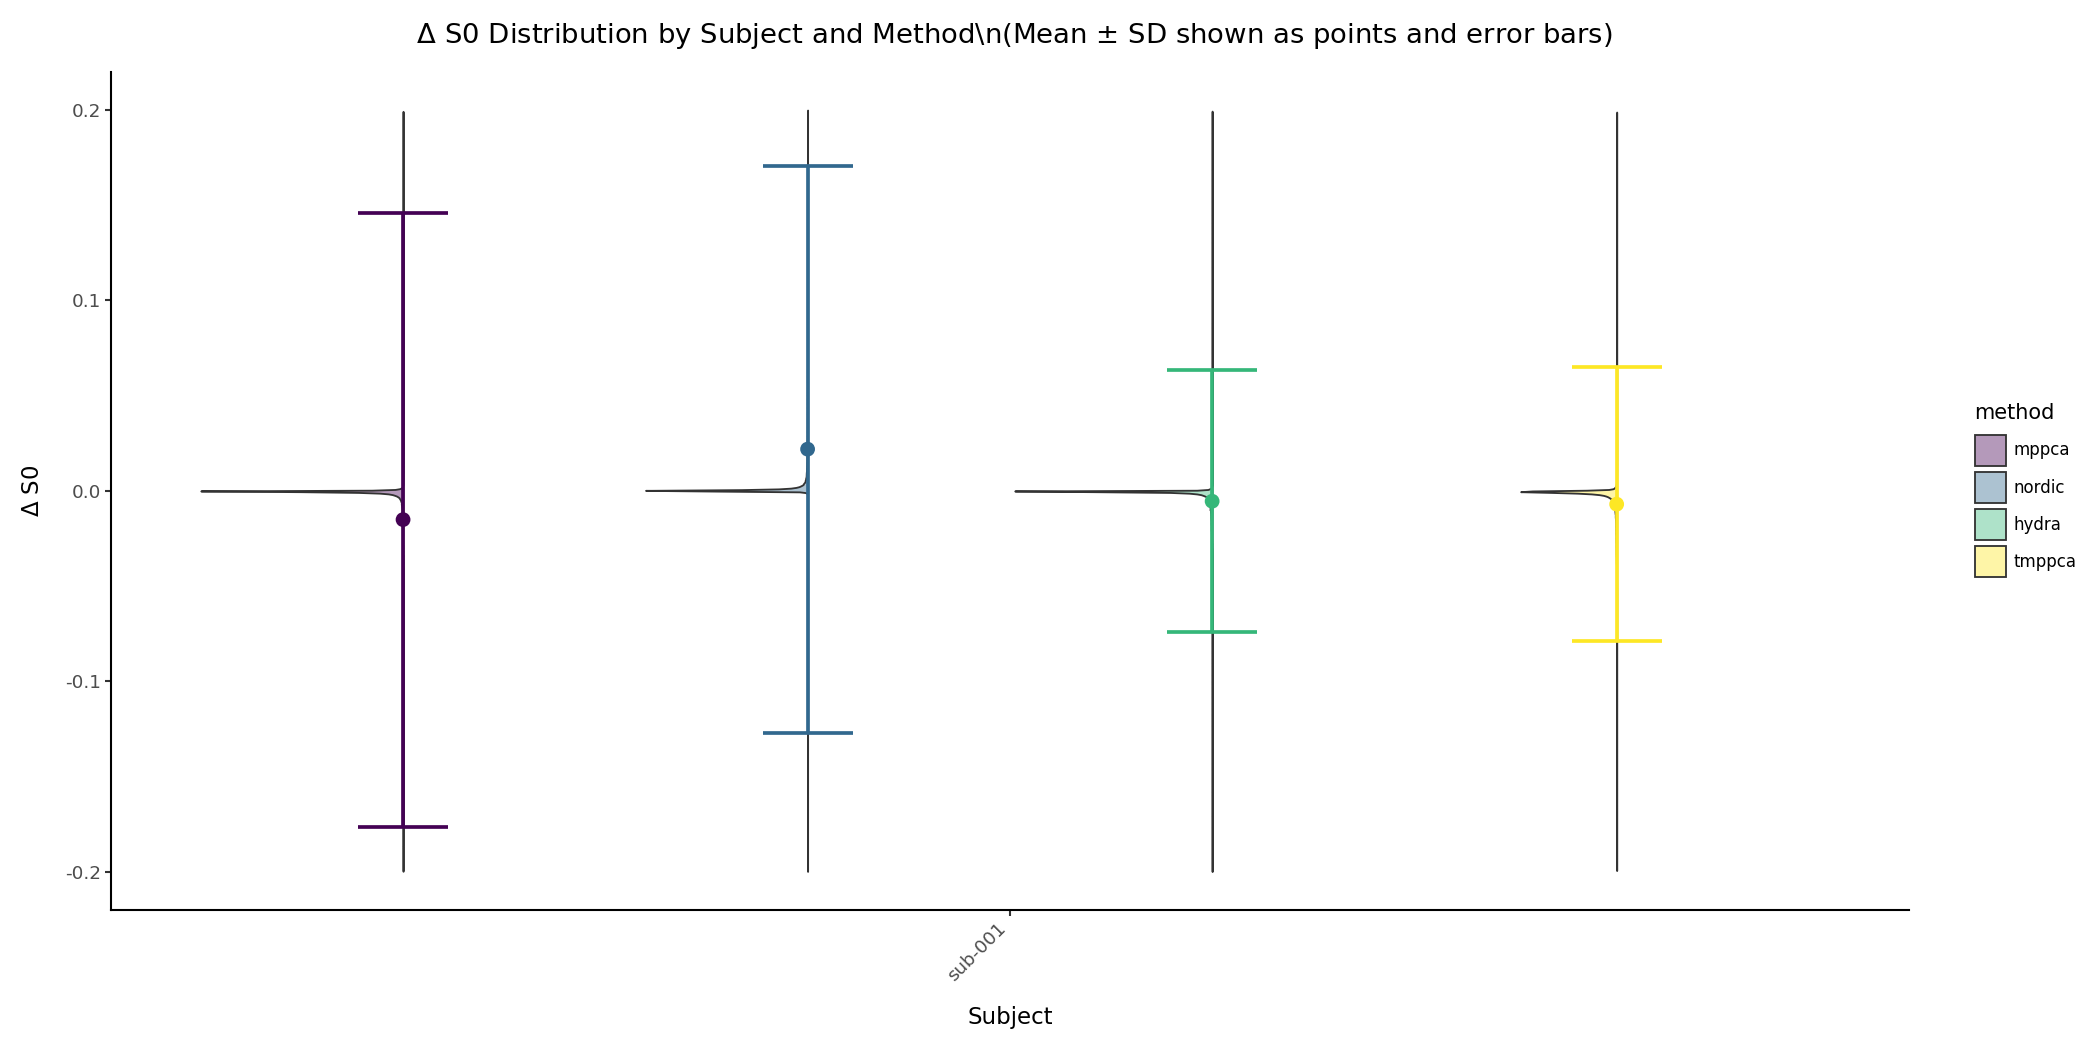
\includegraphics[width=7cm]{images/halfviolin_s0spc_across_subjects_maskedHR.png} \\
    \end{tabular}
    }
    \centering
    \caption[Distribution of changes in $S0$  per dataset]{Histograms of $\Delta S_0$ ( change relative to vanilla).}
    \label{fig:boxplotS0spc}
\end{figure}

\subsection{Net magnetization estimates ($S_0$)}
To assess whether the denoising methods under investigation alter the estimation of net magnetization, we compared the arbitrary $S_0$ values derived from TEDANA. As expected, across all three datasets (the left panel show mean $S_0$ estimates, while the right panel show the relative difference, $\Delta S_0$, between each strategy and the vanilla approach; 2.4 mm, Fig.~\ref{fig:S01200}; 2 mm, Fig.~\ref{fig:S01700}; 1.5 mm, Fig.~\ref{fig:S0hr}), brain regions characterized by lower SNR due to their distance from the receive coils exhibited lower $S_0$ estimates. Conversely, areas proximal to the coils displayed the highest signal intensity, consistent with their higher SNR profile.

Qualitatively, no substantial differences in $S_0$ estimates are observed across methods or datasets. Given the $T_2^*$-weighted combination, this suggests that the underlying signal contributions across echoes remain largely consistent regardless of the denoising strategy.  Overall, only negligible changes are observed. In frontal regions and white matter, NORDIC and HYDRA exhibit slight overestimations, whereas MPPCA and TMPPCA exhibit underestimations. This is consistent with the $\overline{R_2^*}$ analysis that revealed a comparable spatial pattern in these areas.

Examining the signal change between the vanilla and denoised conditions revealed a consistent pattern in the high SNR datasets. For the 2.4 and 2 mm resolutions, NORDIC and HYDRA yielded slight increases in $S_0$ signal intensity near the ventricles and toward the temporal lobes, whereas MPPCA and TMPPCA showed modest signal decreases in these same regions. For the 1.5 mm dataset, only NORDIC produced a slight increase in $S_0$, while the rest of denoising approaches exhibited comparable signal decreases.

Despite these regional variations, the overall distribution of $S_0$ values remained remarkably similar across all datasets and denoising methods (Fig.~\ref{fig:boxplotS0}). Minor changes were nonetheless evident in the $\Delta S_0$ histograms (Fig.~\ref{fig:boxplotS0spc}) , which revealed that while all methods produced generally negligible changes, TMPPCA exhibited the smallest distribution tails.

% Reliability
\subsection{Functional Connectivity Reliability Analysis}


Next, we evaluated whether thermal denoising enhances the reliability of functional connectivity (FC) mapping. The underlying premise is that reducing random variance from thermal sources yields more stable signal estimates, thereby facilitating consistent characterization of voxel‑wise relationships. At coarser spatial resolutions, thermal noise is less dominant; consequently, other confounds (e.g., motion, physiological fluctuations) become more prominent (Sec.~\ref{sec:noiseMRI}). In this context, FC analysis tests whether the assumption of voxel‑wise signal identity—that a given voxel exhibits a consistent signal profile across observations—holds more strongly after denoising. However, FC reliability alone cannot determine whether the removed variance is specifically thermal. This motivated our independent preprocessing of split‑half datasets and subsequent FC analysis (Fig.~\ref{fig:preprocessing}).

Reliability scores increased with voxel size: 2.4 mm (Fig.~\ref{fig:reliability1200})$ >$ 2 mm (Fig.~\ref{fig:reliability1700})$ >$ 1.5 mm (Fig.~\ref{fig:reliabilityHR}). We attribute this improvement to the reduction of non‑neurobiological signal components, which enhances signal stability and renders voxel‑wise relationships more readily characterizable.

For the low‑resolution datasets (2.4 mm and 2 mm), a consistent ranking emerged: TMPPCA $>$ NORDIC $>$ HYDRA $>$ MPPCA $>$ vanilla (Fig.~\ref{fig:reliabilityFC}, left panels). For the high‑resolution dataset (1.5 mm), the pattern differed: TMPPCA $>$ NORDIC $>$ HYDRA $\approx$ MPPCA $>$ vanilla. This divergence aligns with the tSNR analysis: forcing spatial redundancy by concatenating echoes negatively impacts signal quality when thermal noise dominates high‑resolution acquisitions. The right panels of Fig.~\ref{fig:reliabilityFCspc} show that $\Delta r^2$ distributions are consistently and positively skewed.

Across all datasets, undenoised data showed the highest $r^2$ values in regions near the head coils. With increasing denoising efficacy, the spatial distribution of $r^2$ saturation progressively shifted and expanded throughout gray matter, indicating enhanced signal fidelity. Practically, this suggests that thermal denoising is particularly beneficial for frontal and temporal lobes. The pronounced improvement with TMPPCA supports its feasibility for enhancing FC data quality.


\begin{figure}[htbp]
\centering \colorbox{black}{
    \centering
    \begin{tabular}{>{\centering\arraybackslash}m{1cm}>{\centering\arraybackslash}m{3cm}>{\centering\arraybackslash}m{3cm}}
       & \textcolor{white}{\textbf{VANILLA}} & \textcolor{white}{\textbf{MPPCA}} \\
    &    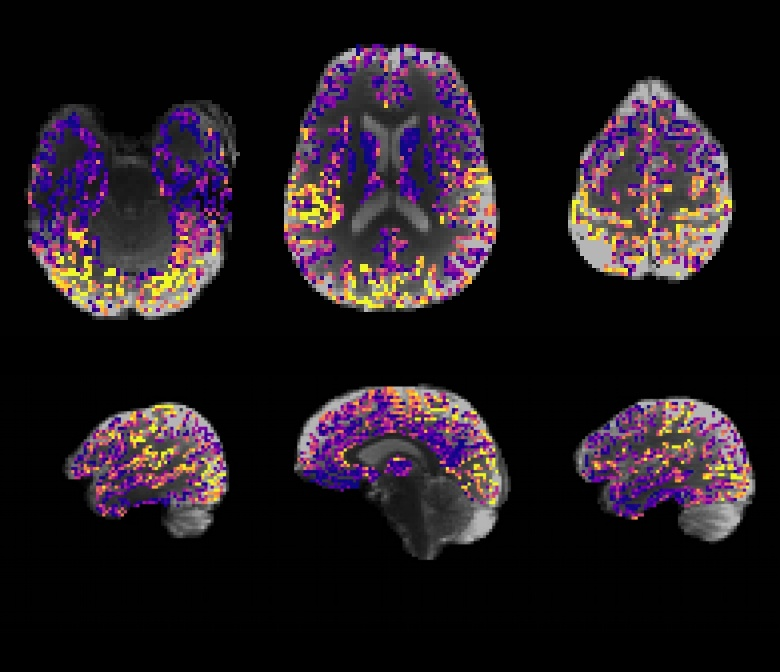
\includegraphics[width=3cm]{images/sub-001_ses-1_task-HABLA1200_OC_part-mag_bold_vanilla01_all.jpg} &
        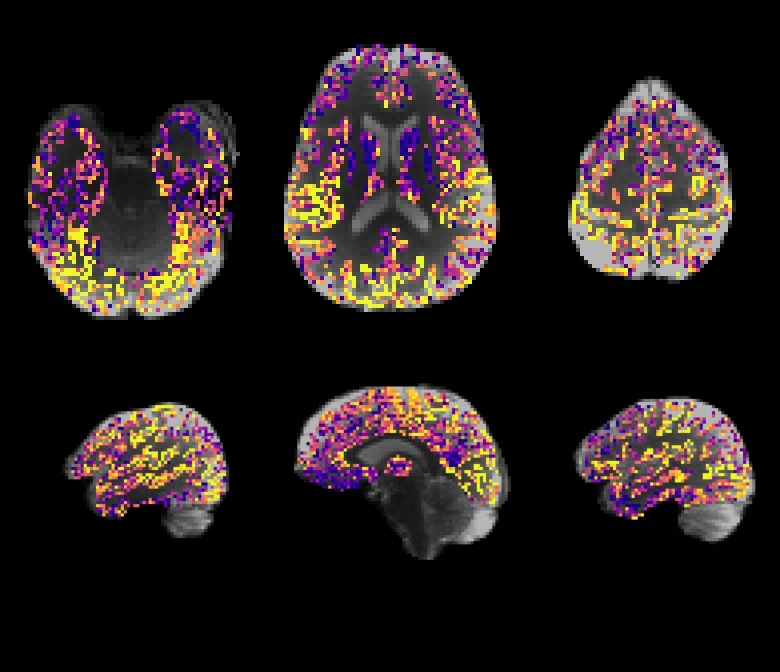
\includegraphics[width=3cm]{images/sub-001_ses-1_task-HABLA1200_OC_part-mag_bold_mppca01_all.jpg}\\
      &   \textcolor{white}{\textbf{NORDIC}}& \textcolor{white}{\textbf{HYDRA}}\\
        \includegraphics[width=.5cm]{images/PlasmaR2.png}&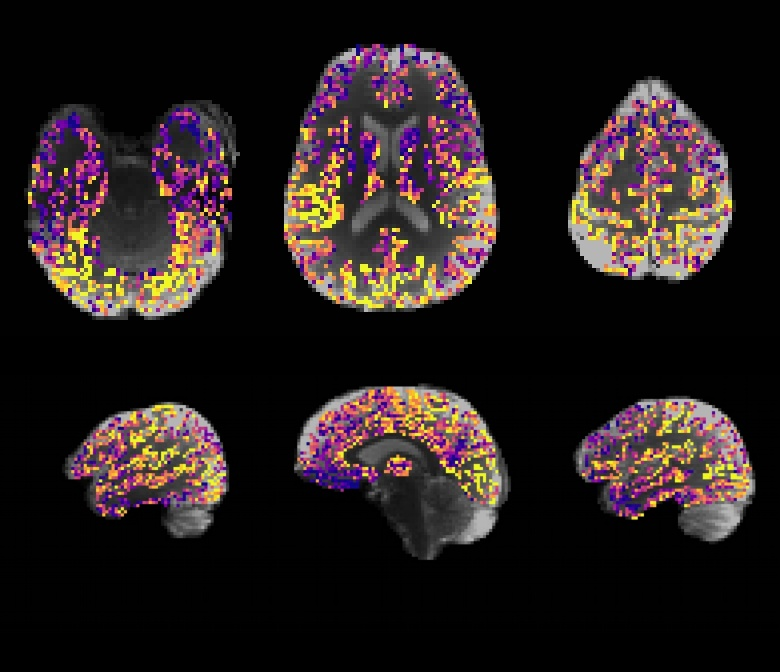
\includegraphics[width=3cm]{images/sub-001_ses-1_task-HABLA1200_OC_part-mag_bold_nordic01_all.jpg} &
        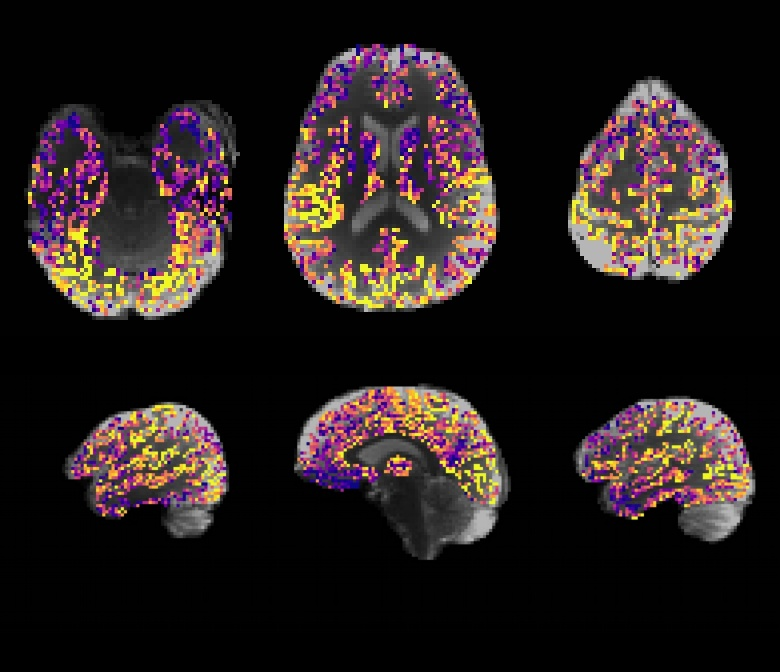
\includegraphics[width=3cm]{images/sub-001_ses-1_task-HABLA1200_OC_part-mag_bold_hydra01_all.jpg}\\
          &       \multicolumn{2}{c}{\textcolor{white}{\textbf{TMPPCA}}}\\
      &  \multicolumn{2}{c}{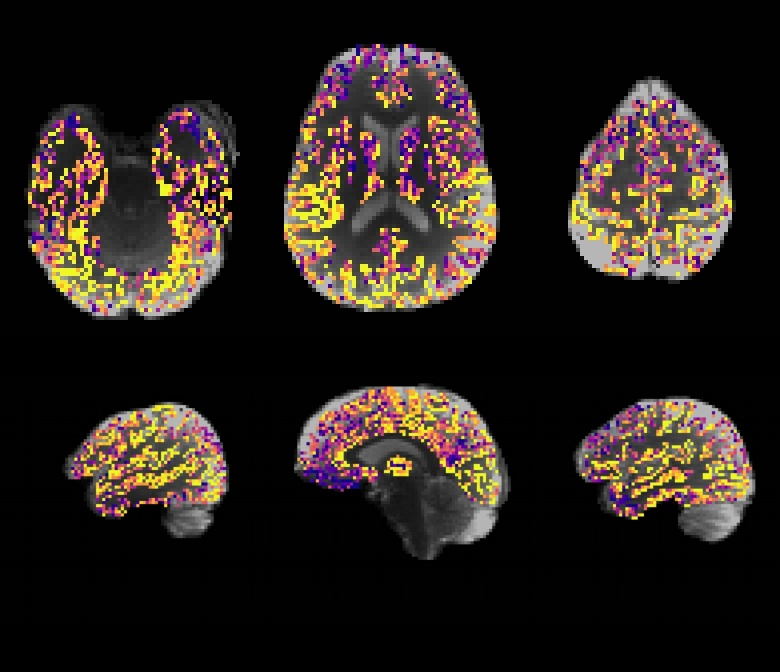
\includegraphics[width=3cm]{images/sub-001_ses-1_task-HABLA1200_OC_part-mag_bold_tmppca01_all.jpg}} \\
    \end{tabular}
    }
    \caption[Functional connectivity reliability maps at low resolution (2.4 mm isotropic)]{Functional connectivity reliability maps ($r^2$) obtained with 2.4 mm isotropic dataset for a representative subject.}
    \label{fig:reliability1200}
\end{figure}

\begin{figure}[htbp]
\centering \colorbox{black}{
    \centering
    \begin{tabular}{>{\centering\arraybackslash}m{1cm}>{\centering\arraybackslash}m{3cm}>{\centering\arraybackslash}m{3cm}}
       & \textcolor{white}{\textbf{VANILLA}} & \textcolor{white}{\textbf{MPPCA}} \\
    &    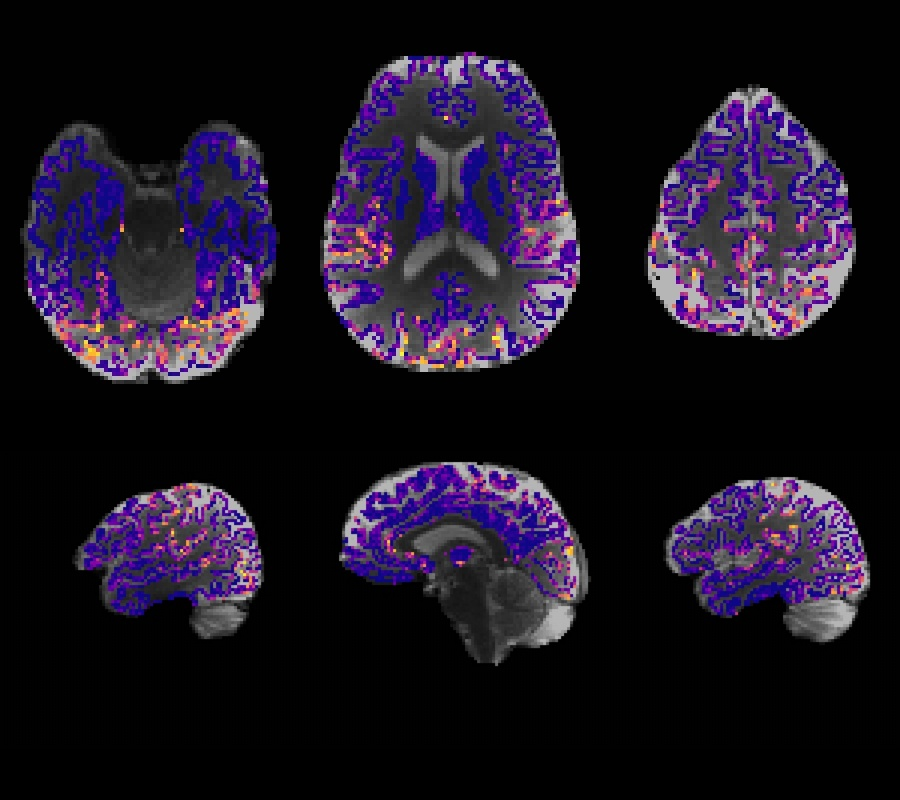
\includegraphics[width=3cm]{images/sub-001_ses-1_task-HABLA1700_OC_part-mag_bold_vanilla01_all.jpg} &
        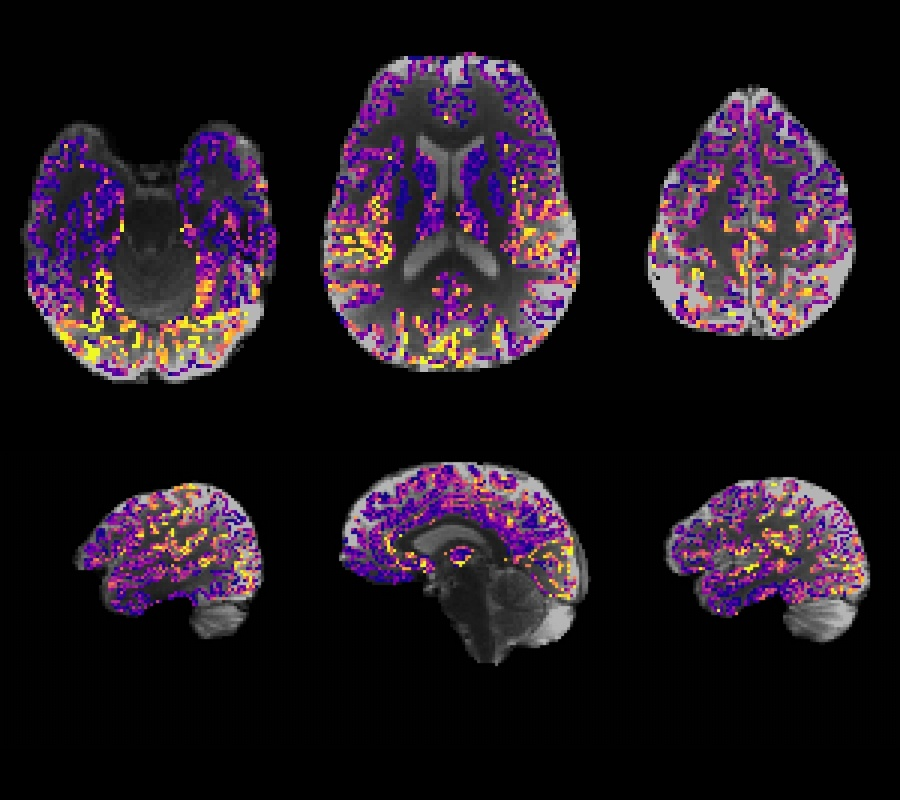
\includegraphics[width=3cm]{images/sub-001_ses-1_task-HABLA1700_OC_part-mag_bold_mppca01_all.jpg}\\
      &   \textcolor{white}{\textbf{NORDIC}}& \textcolor{white}{\textbf{HYDRA}}\\
        \includegraphics[width=.5cm]{images/PlasmaR2.png}&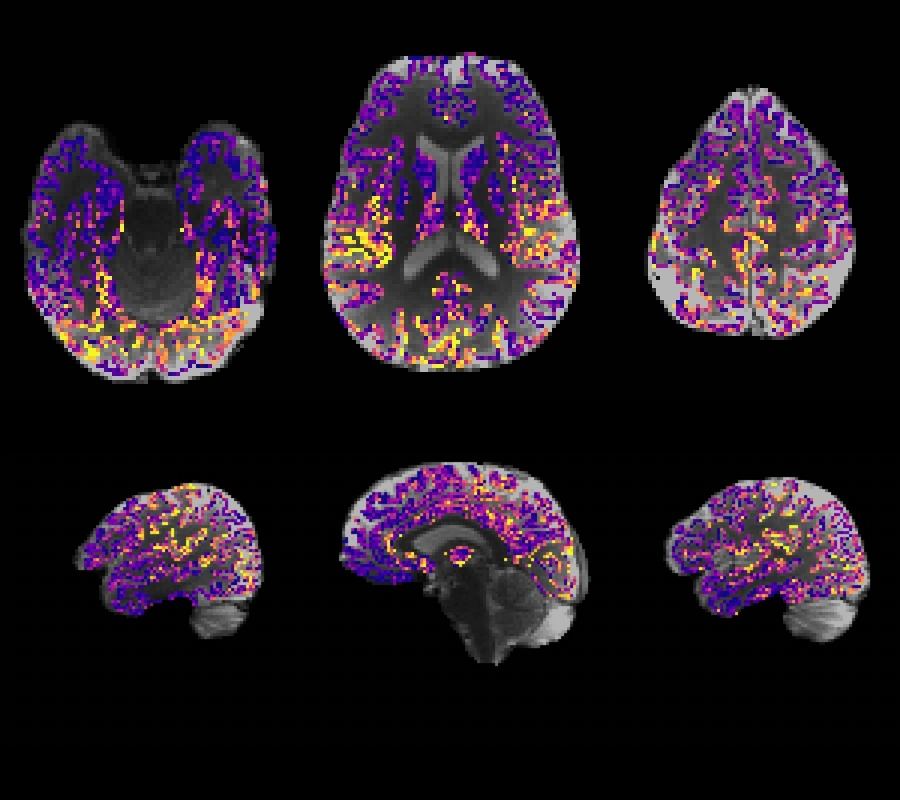
\includegraphics[width=3cm]{images/sub-001_ses-1_task-HABLA1700_OC_part-mag_bold_nordic01_all.jpg} &
        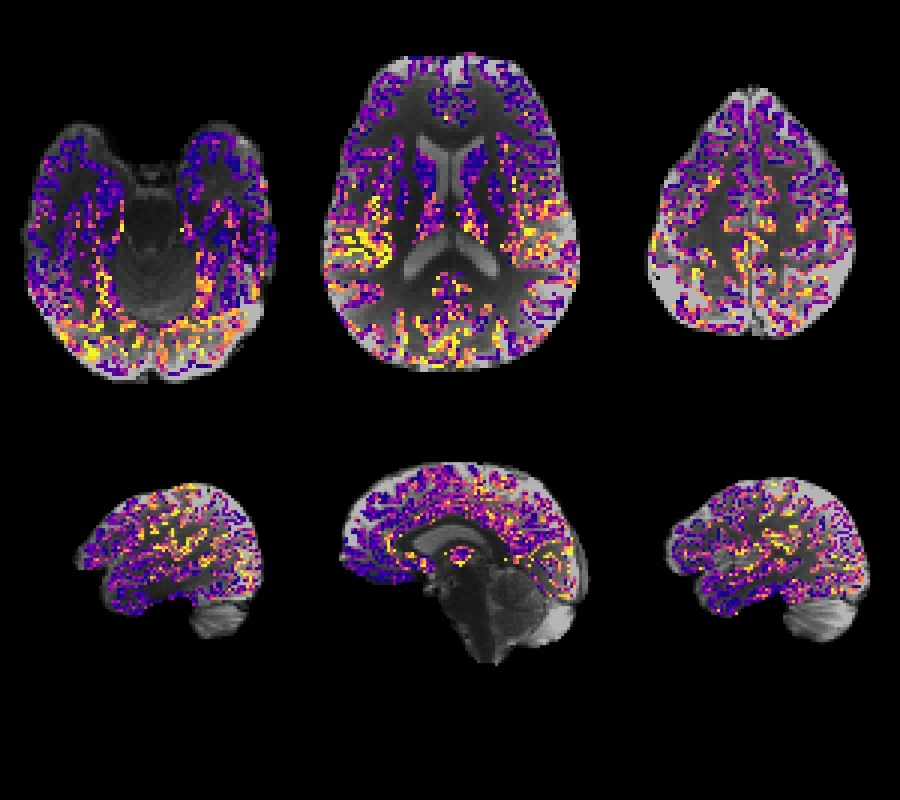
\includegraphics[width=3cm]{images/sub-001_ses-1_task-HABLA1700_OC_part-mag_bold_hydra01_all.jpg}\\
          &       \multicolumn{2}{c}{\textcolor{white}{\textbf{TMPPCA}}}\\
      &  \multicolumn{2}{c}{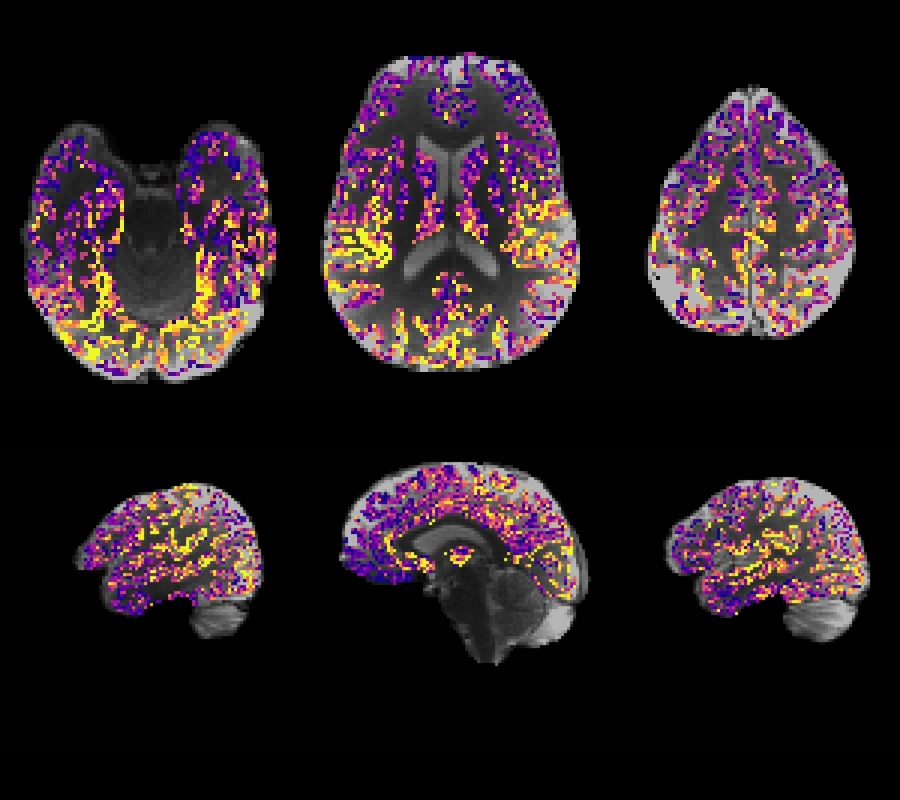
\includegraphics[width=3cm]{images/sub-001_ses-1_task-HABLA1700_OC_part-mag_bold_tmppca01_all.jpg}} \\
    \end{tabular}
    }
    \caption[Functional connectivity reliability maps at low resolution (2 mm isotropic)]{Functional connectivity reliability maps ($r^2$) obtained with 2 mm isotropic dataset for a representative subject.}
    \label{fig:reliability1700}
\end{figure}

\begin{figure}[htbp]
\centering \colorbox{black}{
    \centering
    \begin{tabular}{>{\centering\arraybackslash}m{1cm}>{\centering\arraybackslash}m{3cm}>{\centering\arraybackslash}m{3cm}}
    
       & \textcolor{white}{\textbf{VANILLA}} & \textcolor{white}{\textbf{MPPCA}} \\
    &    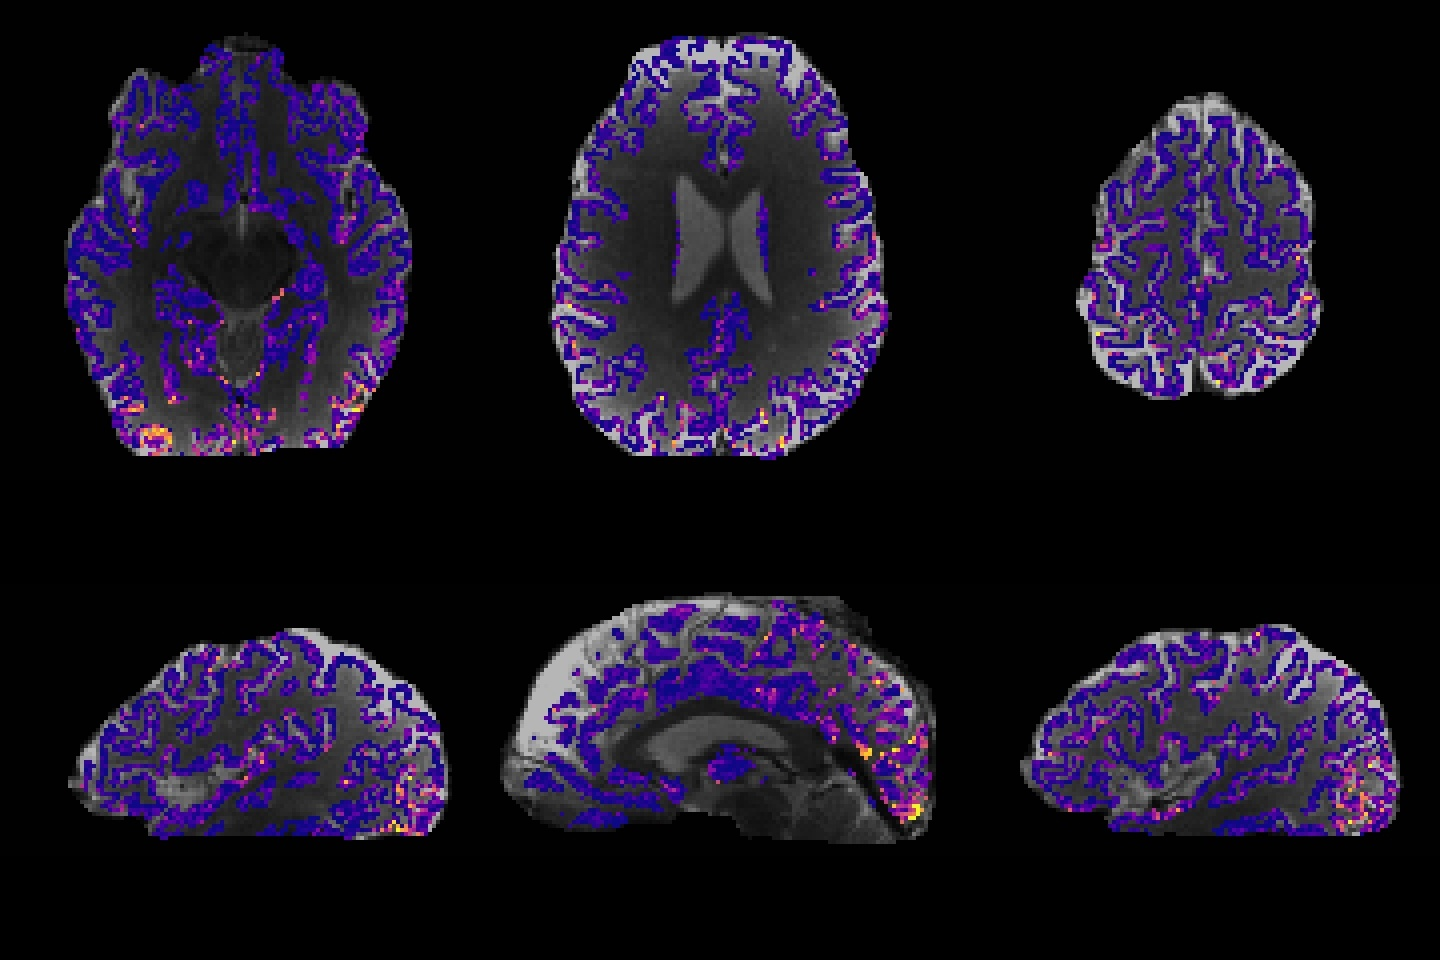
\includegraphics[width=3cm]{images/sub-001_ses-1_task-REST_run-1_OC_part-mag_bold_vanilla01_all.jpg} &
        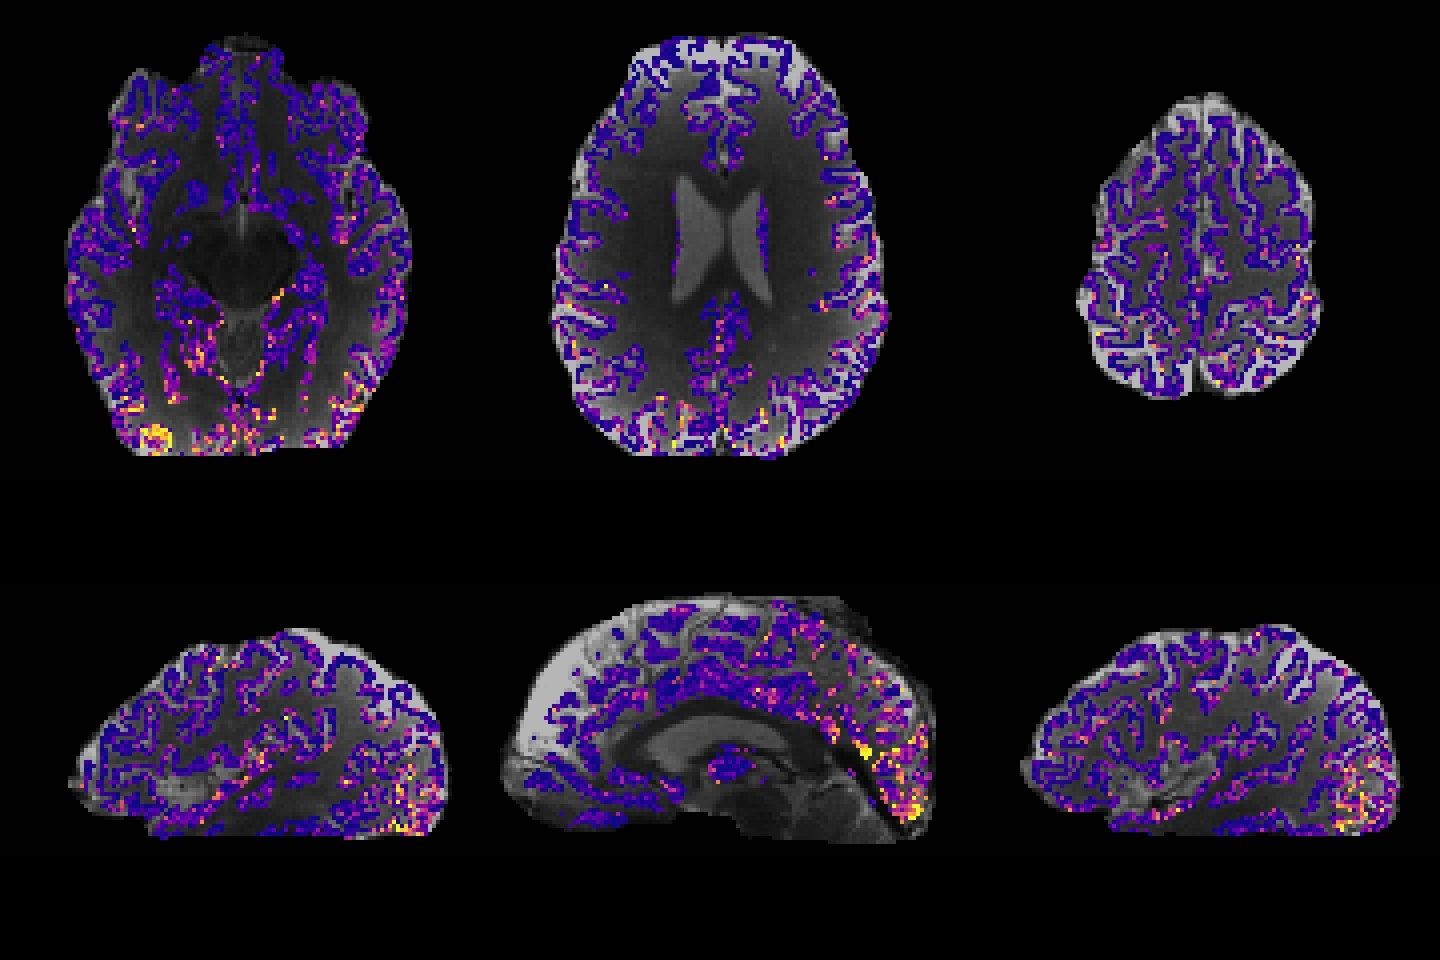
\includegraphics[width=3cm]{images/sub-001_ses-1_task-REST_run-1_OC_part-mag_bold_mppca01_all.jpg}\\
      &   \textcolor{white}{\textbf{NORDIC}}& \textcolor{white}{\textbf{HYDRA}}\\
        \includegraphics[width=.5cm]{images/PlasmaR2.png}&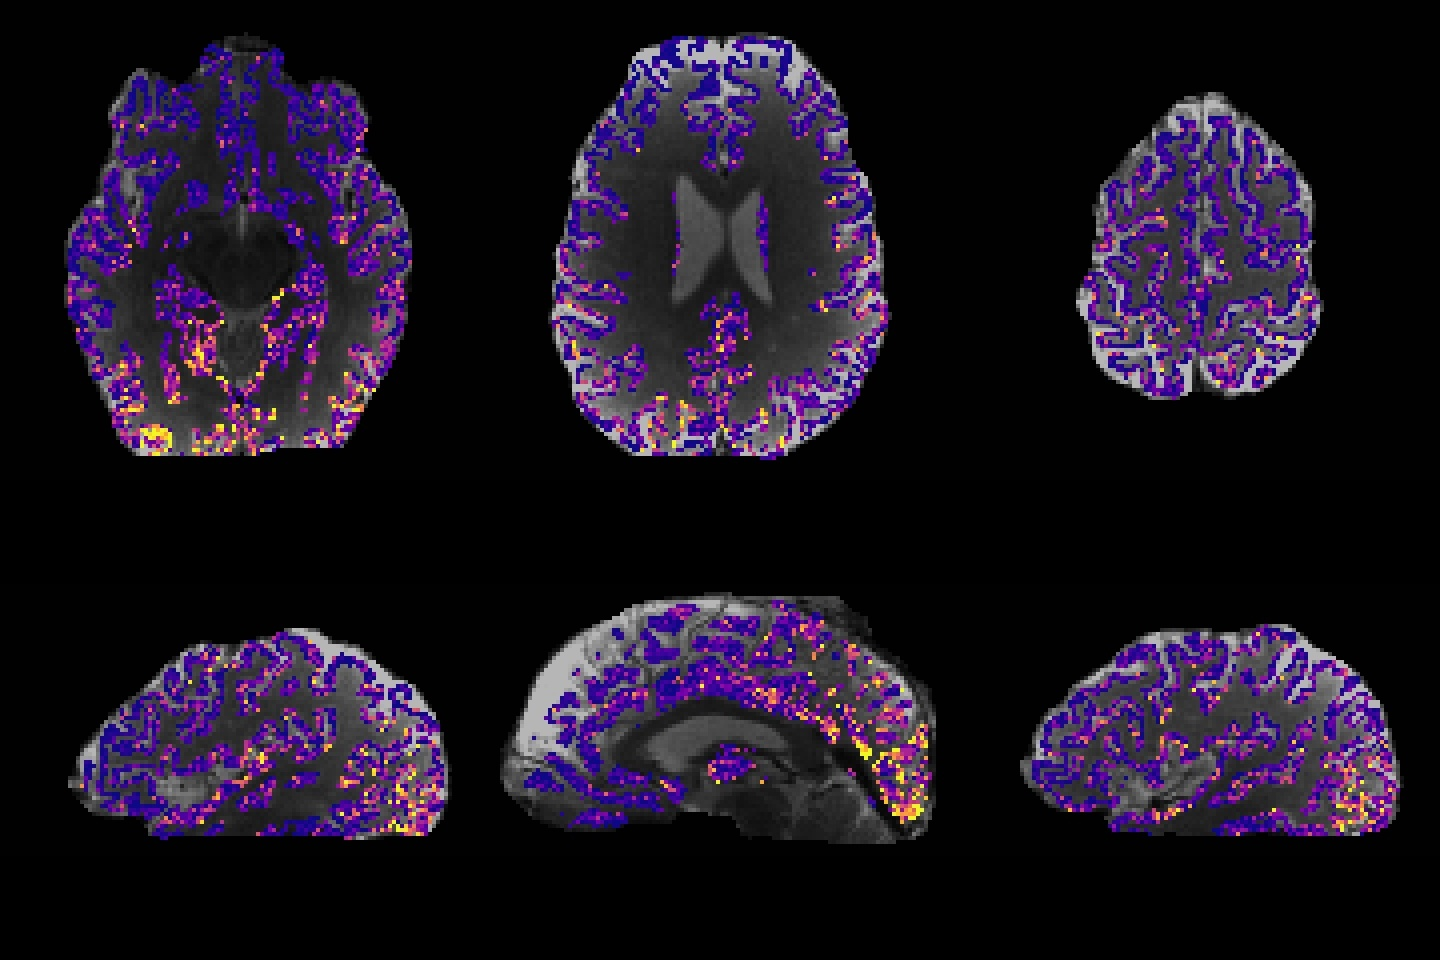
\includegraphics[width=3cm]{images/sub-001_ses-1_task-REST_run-1_OC_part-mag_bold_nordic01_all.jpg} &
        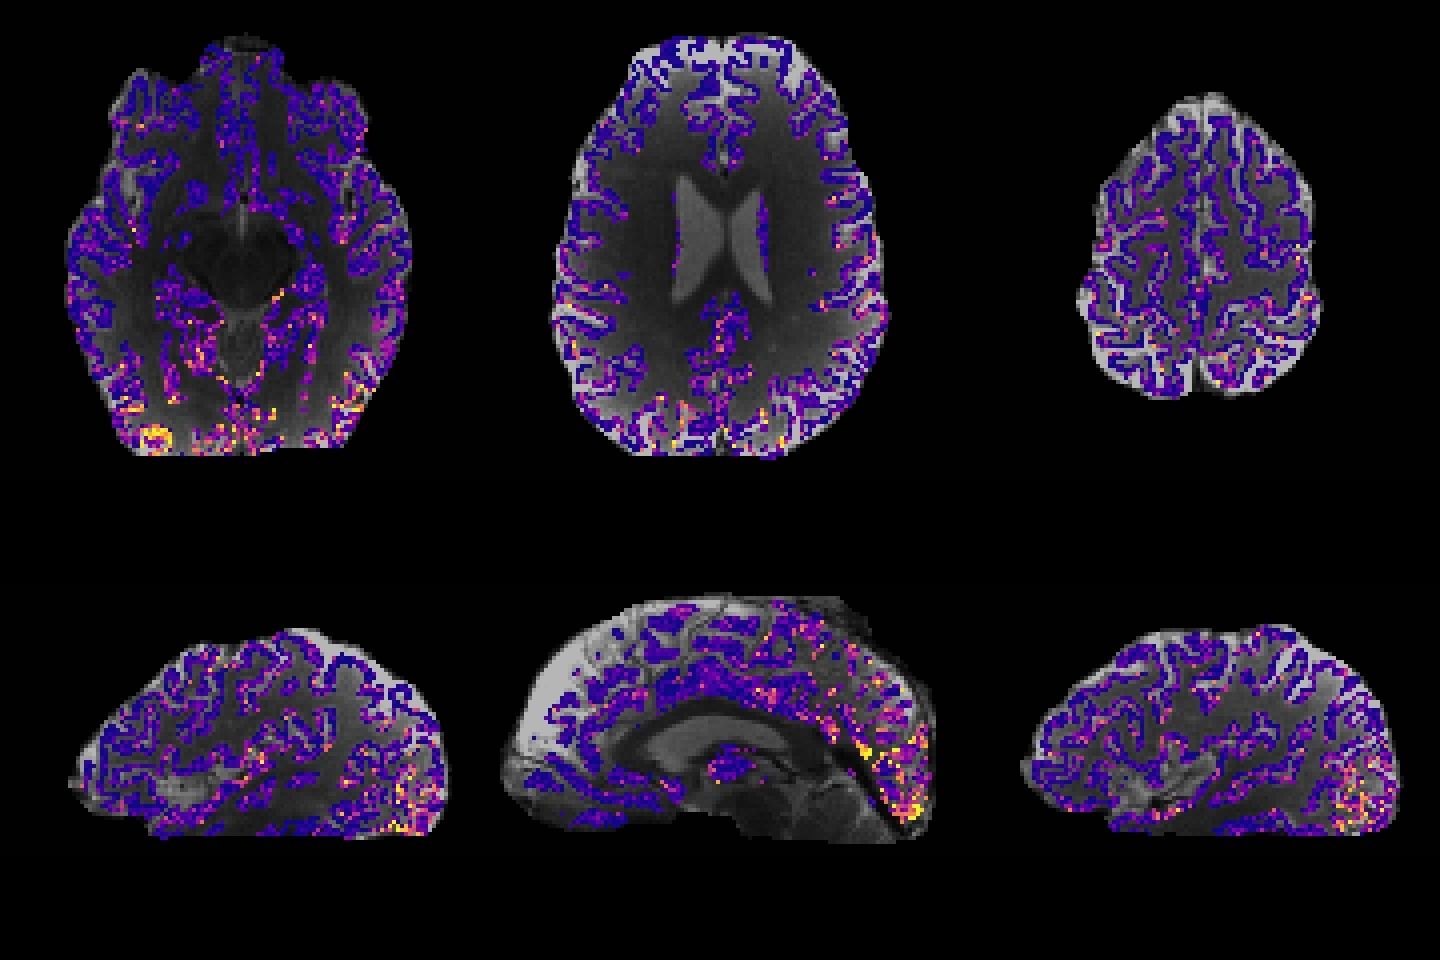
\includegraphics[width=3cm]{images/sub-001_ses-1_task-REST_run-1_OC_part-mag_bold_hydra01_all.jpg}\\
          &       \multicolumn{2}{c}{\textcolor{white}{\textbf{TMPPCA}}}\\
      &  \multicolumn{2}{c}{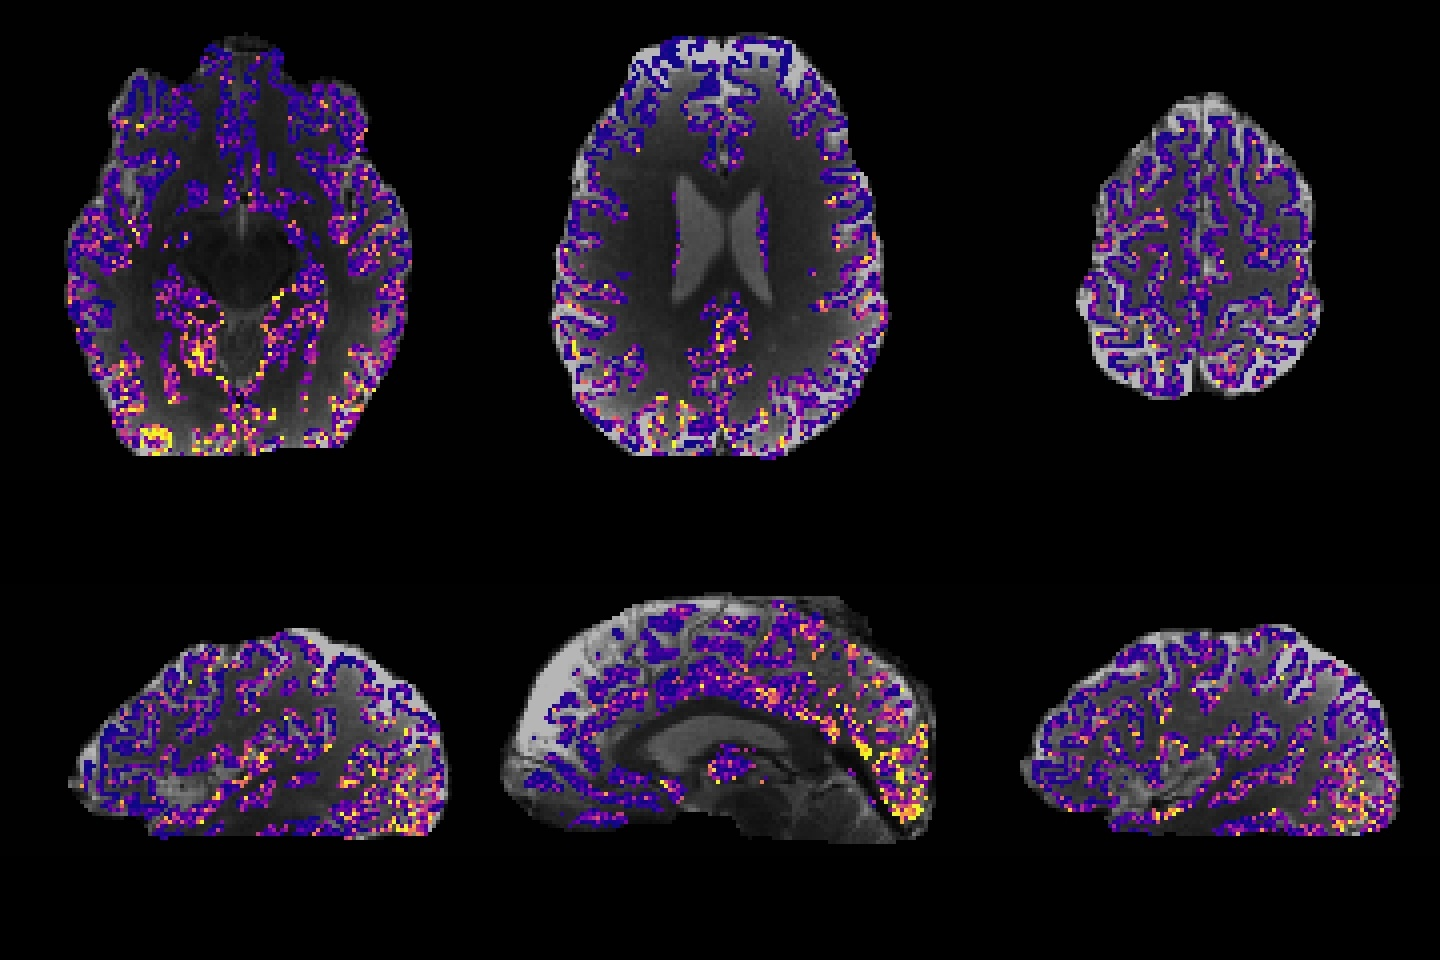
\includegraphics[width=3cm]{images/sub-001_ses-1_task-REST_run-1_OC_part-mag_bold_tmppca01_all.jpg}} \\
    \end{tabular}
    }
    \caption[Functional connectivity reliability maps at high resolution (1.5 mm isotropic)]{Functional connectivity reliability maps ($r^2$) obtained with the 1.5 mm isotropic dataset.}
    \label{fig:reliabilityHR}
\end{figure}

\begin{figure}[htbp]
\raggedleft 
    \centering
    \begin{tabular}{>{\centering\arraybackslash}m{.7cm}>{\centering\arraybackslash}m{7cm}}
       & \textcolor{black}{\textbf{$FC \ reliability \ (r^2)$}}\\
    \rotatebox[origin=l]{90}{\textcolor{black}{2.4 mm}} &    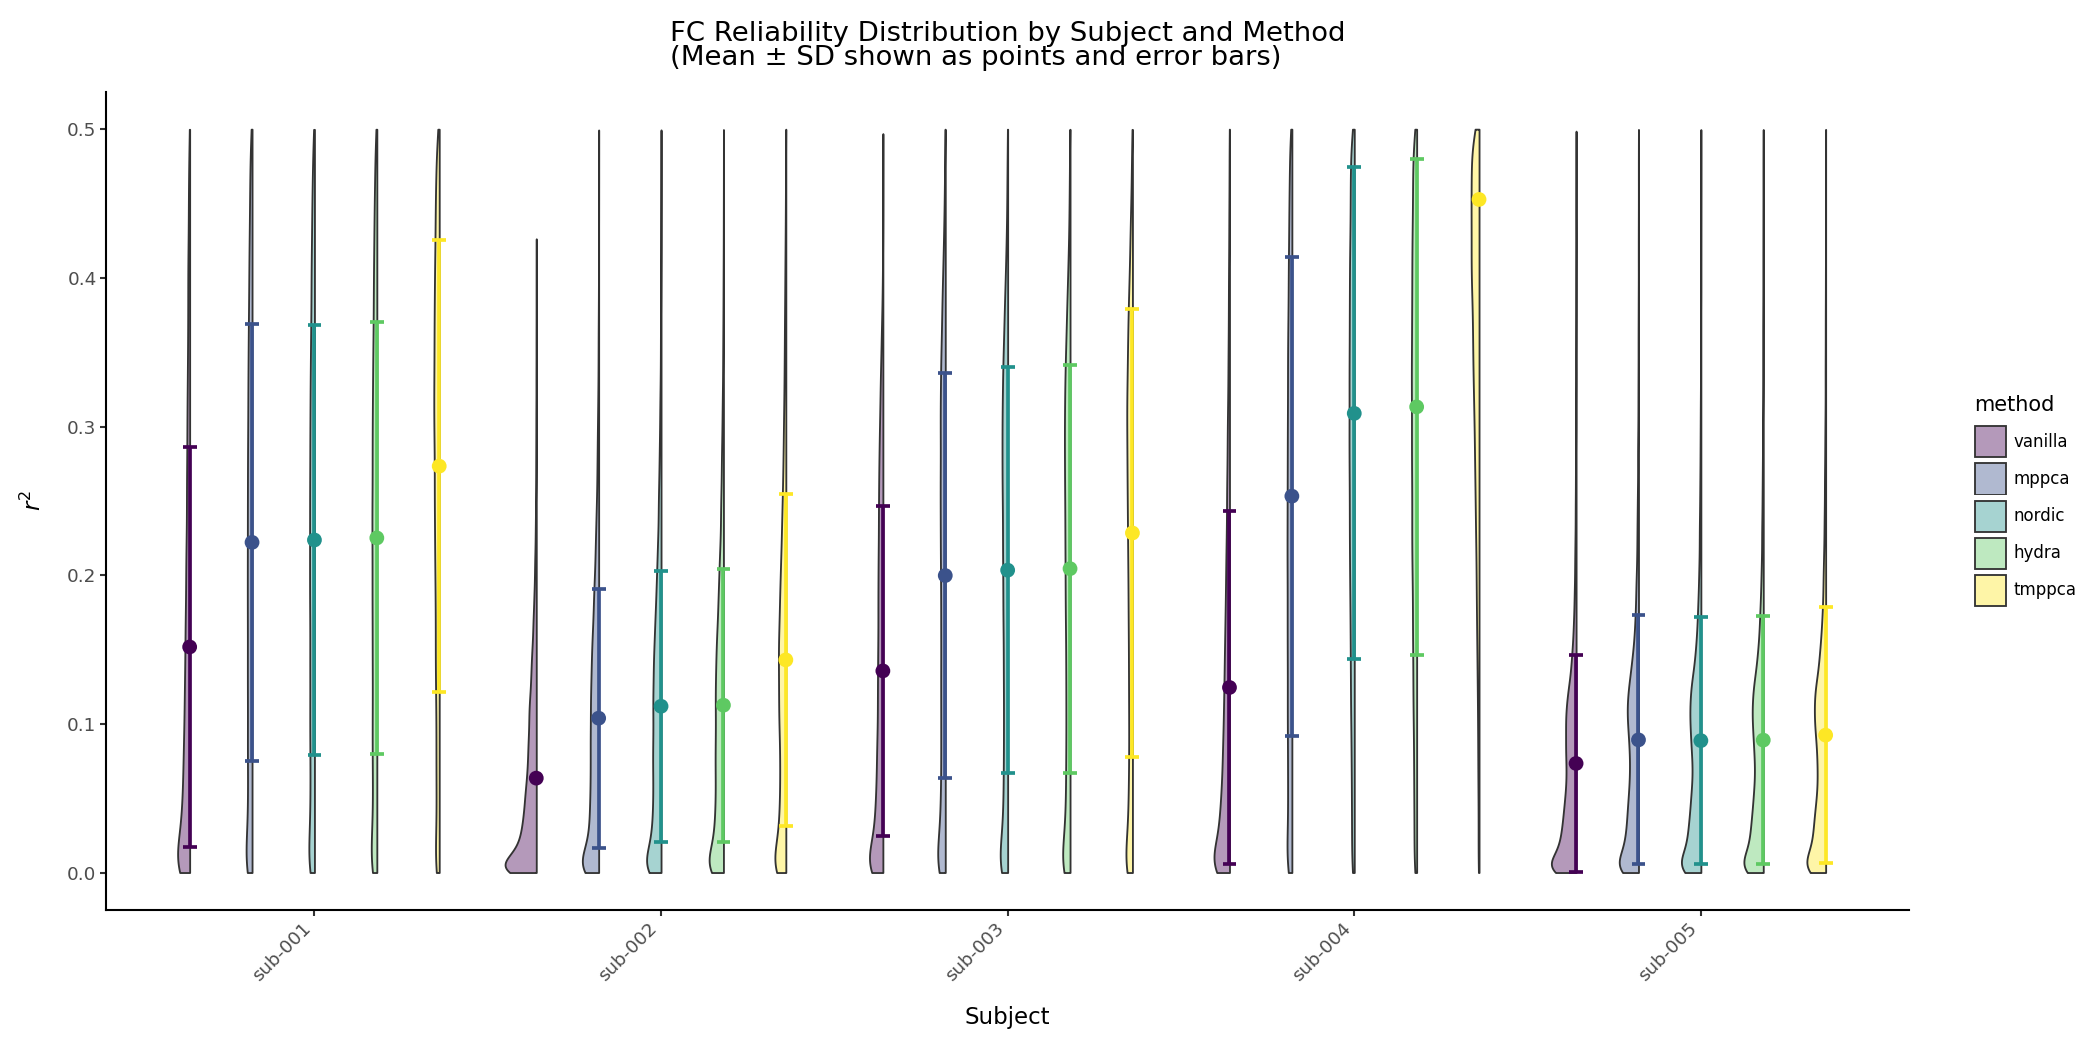
\includegraphics[width=7cm]{images/halfviolin_r2_across_subjects_masked1200.png} \\
       \rotatebox[origin=l]{90}{\textcolor{black}{2 mm}} & 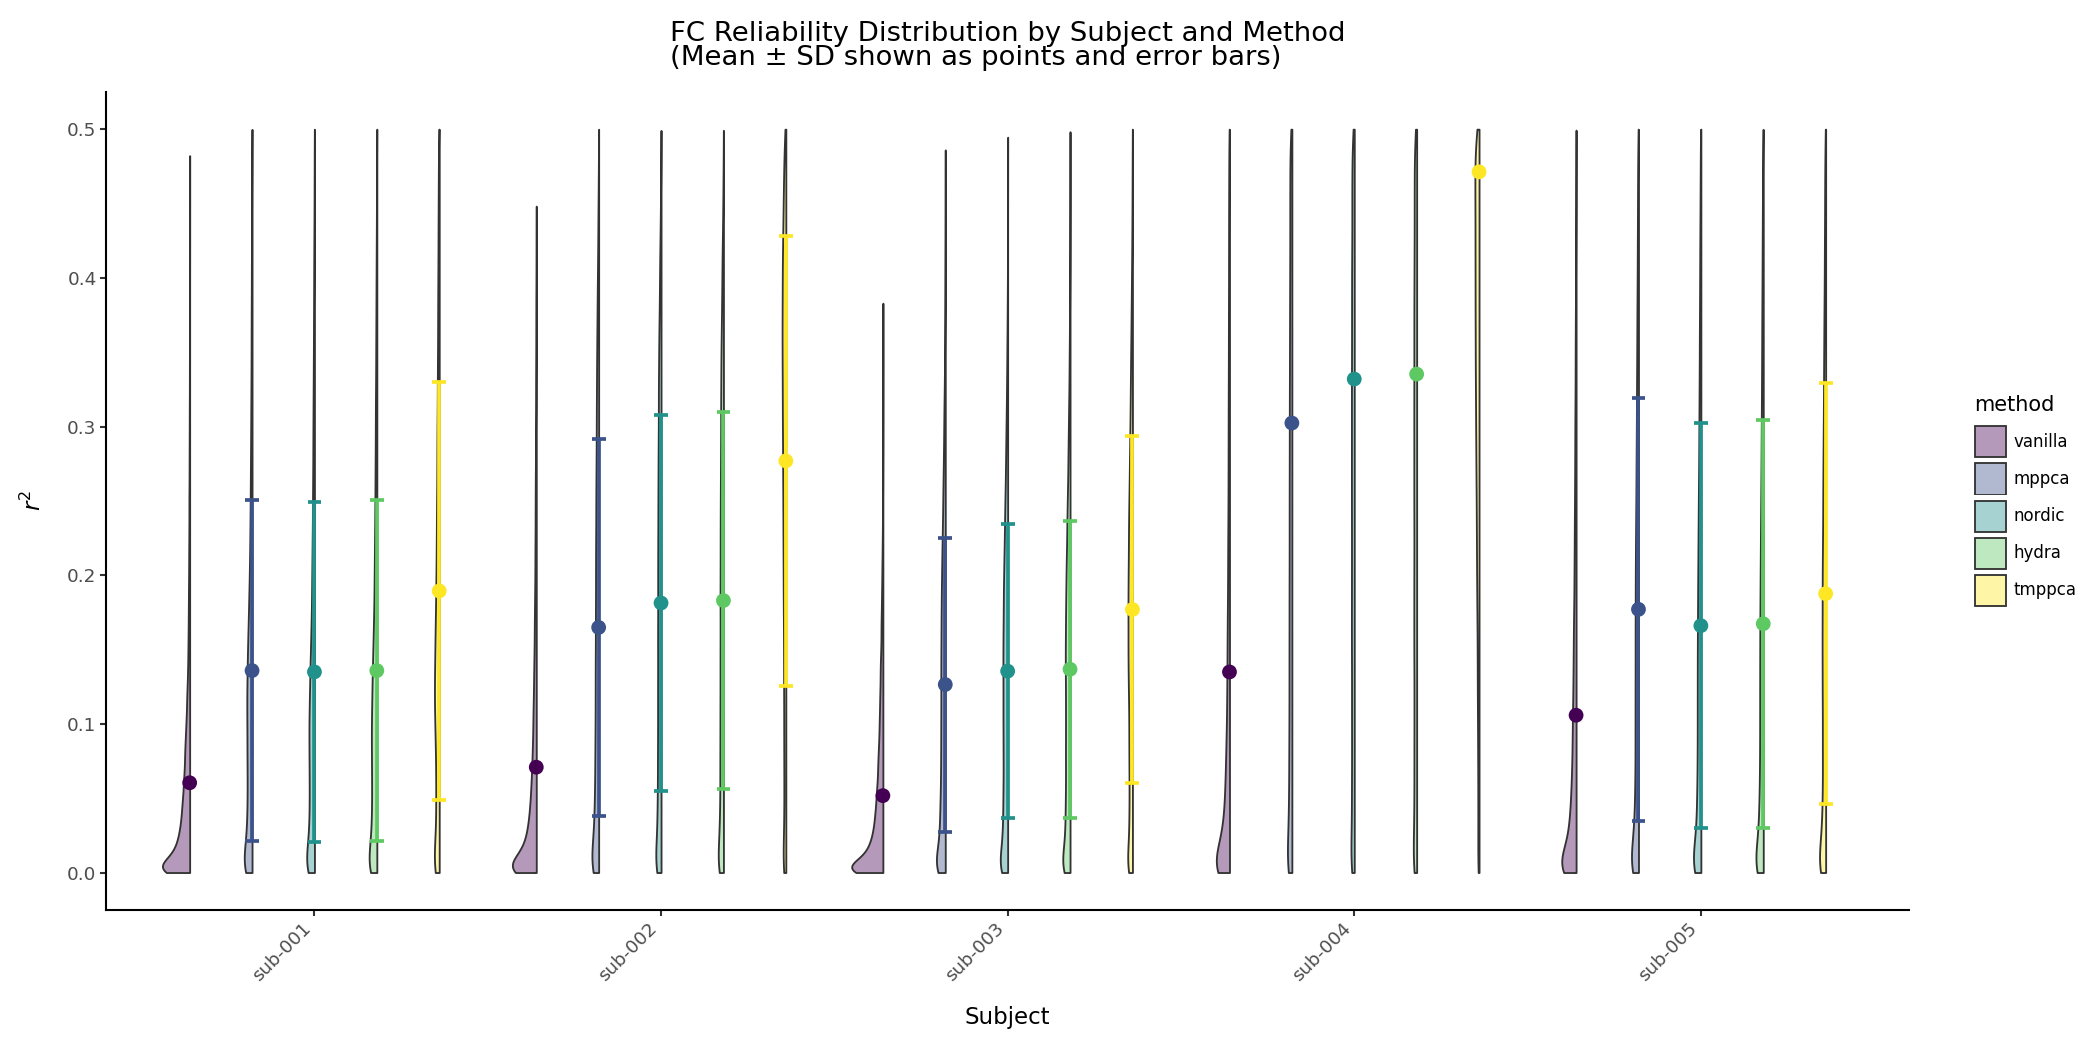
\includegraphics[width=7cm]{images/halfviolin_r2_across_subjects_masked1700.png}\\
      \rotatebox[origin=l]{90}{\textcolor{black}{1.5 mm}}&   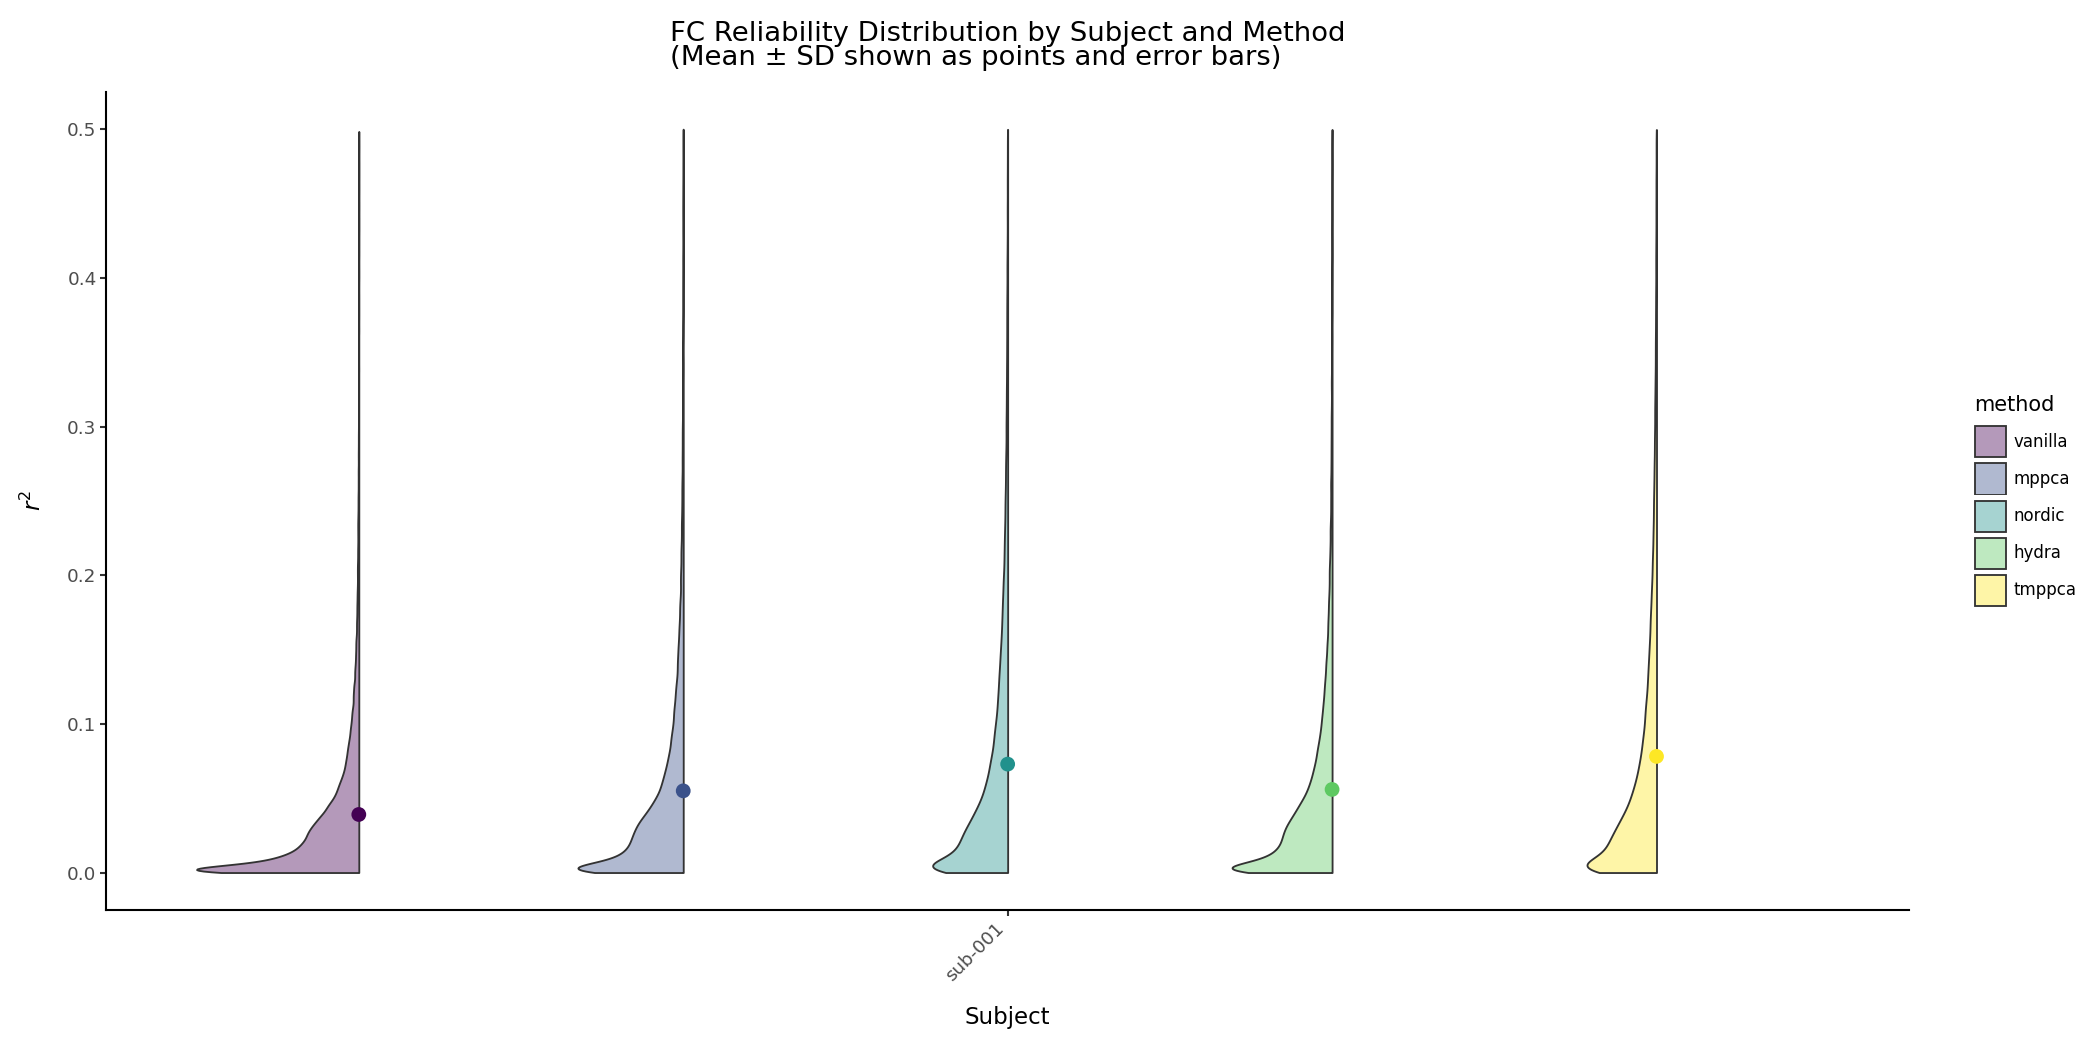
\includegraphics[width=7cm]{images/halfviolin_r2_across_subjects_maskedHR.png} 
    \end{tabular}
    \caption[Distribution of functional connectivity reliability values per dataset ($r^2$)]{ Histograms of functional connectivity reliability ($r^2$) across datasets. }
\label{fig:reliabilityFC}
\end{figure}

\begin{figure}[p]
\raggedleft 
    \centering
    \begin{tabular}{>{\centering\arraybackslash}m{.7cm}>{\centering\arraybackslash}m{7cm}}
        & \textcolor{black}{FC $\Delta r^2$}\\
    \rotatebox[origin=l]{90}{\textcolor{black}{2.4 mm}} & 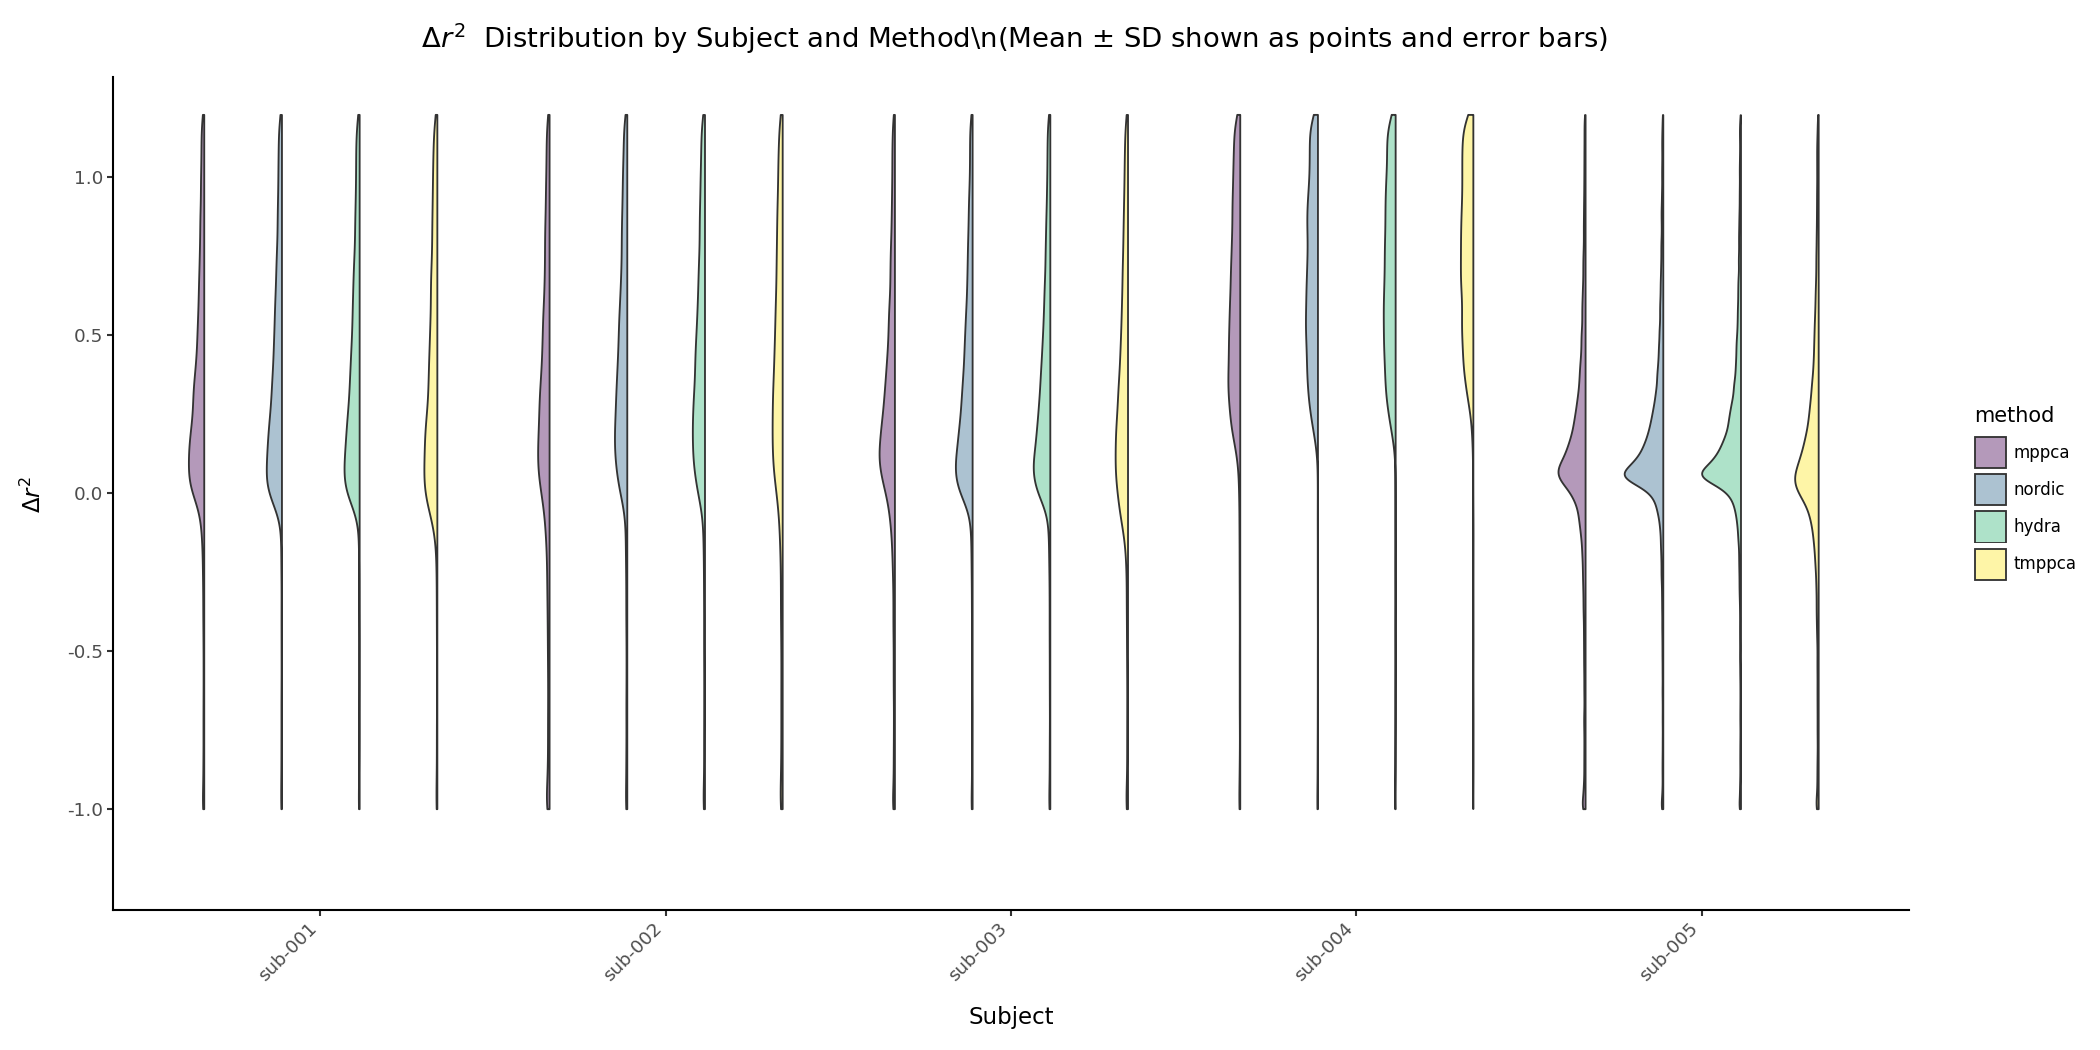
\includegraphics[width=7cm]{images/halfviolin_r2spc_across_subjects_masked1200.png}\\
       \rotatebox[origin=l]{90}{\textcolor{black}{2 mm}} & 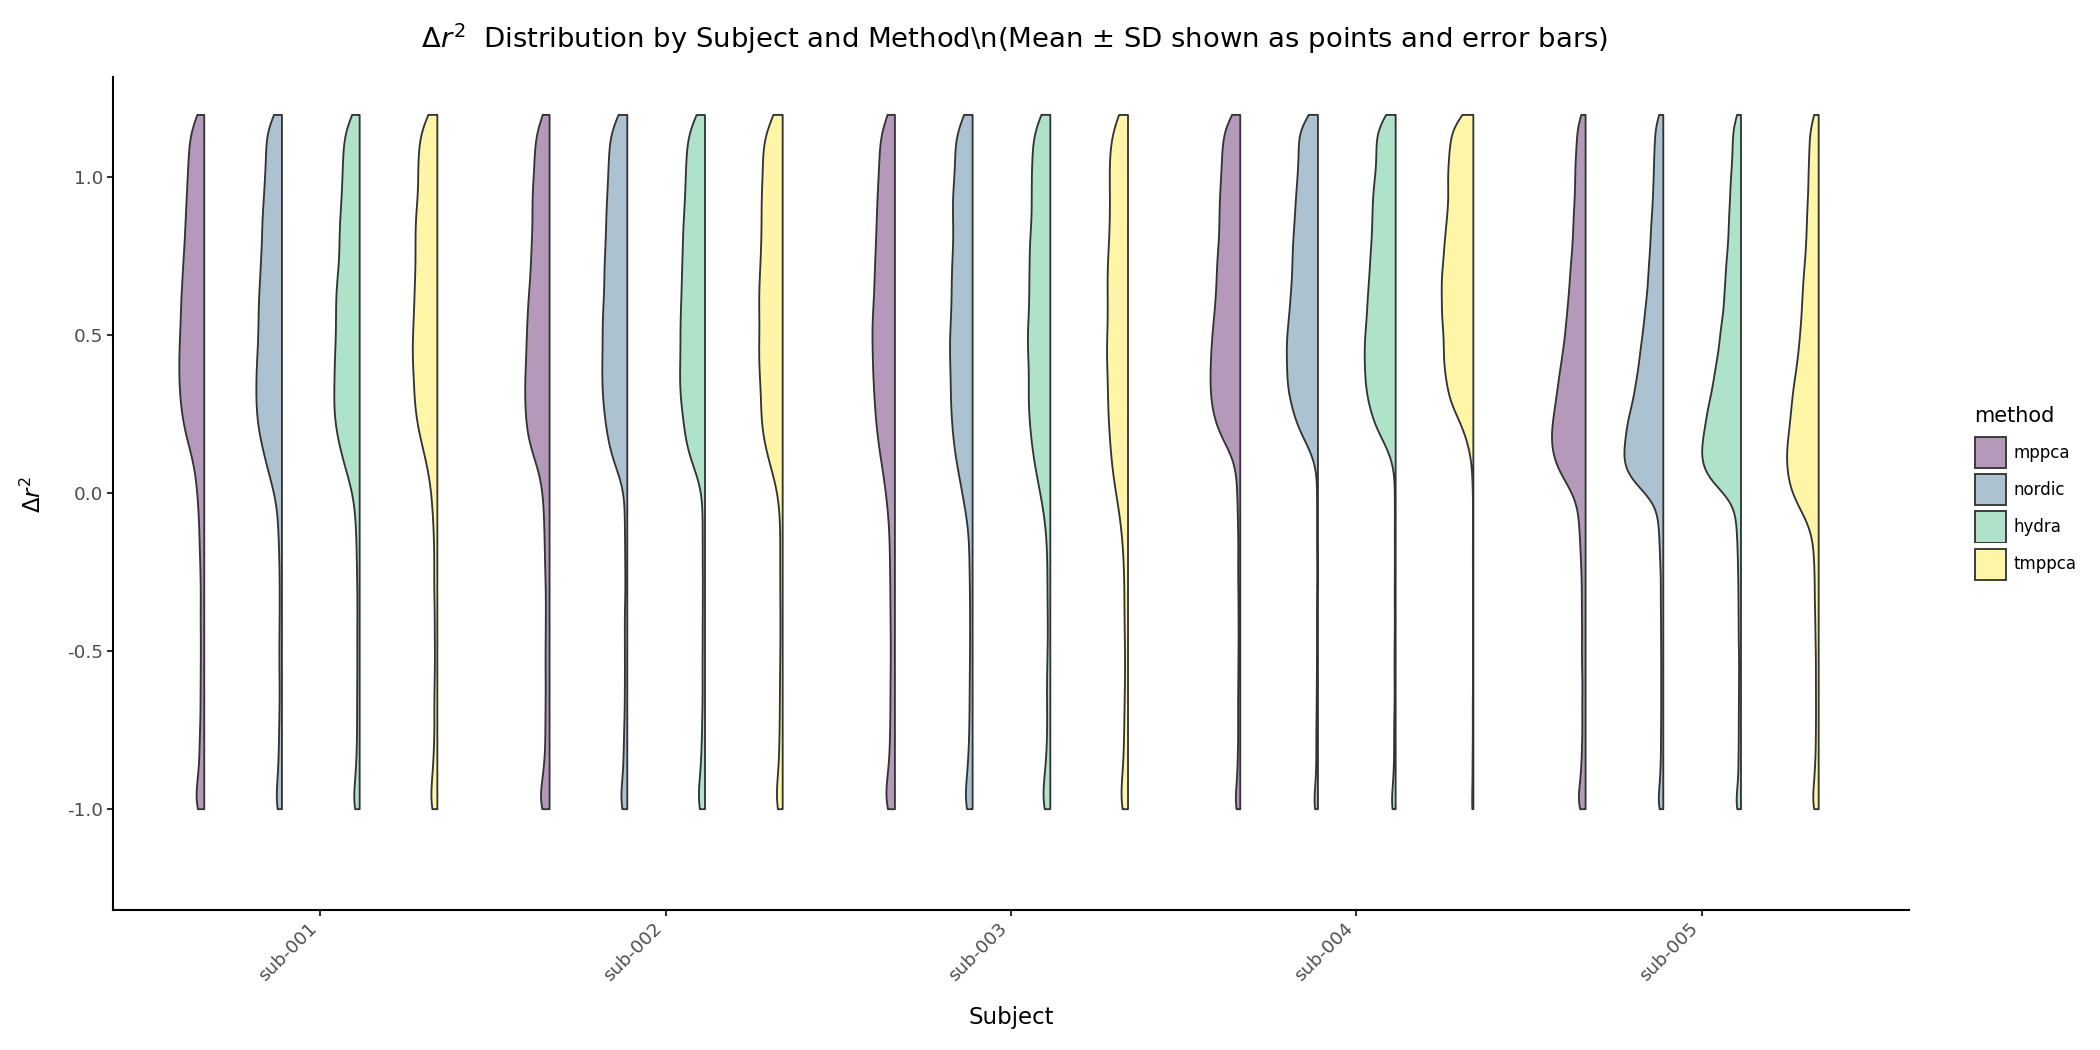
\includegraphics[width=7cm]{images/halfviolin_r2spc_across_subjects_masked1700.png}\\
      \rotatebox[origin=l]{90}{\textcolor{black}{1.5 mm}}& 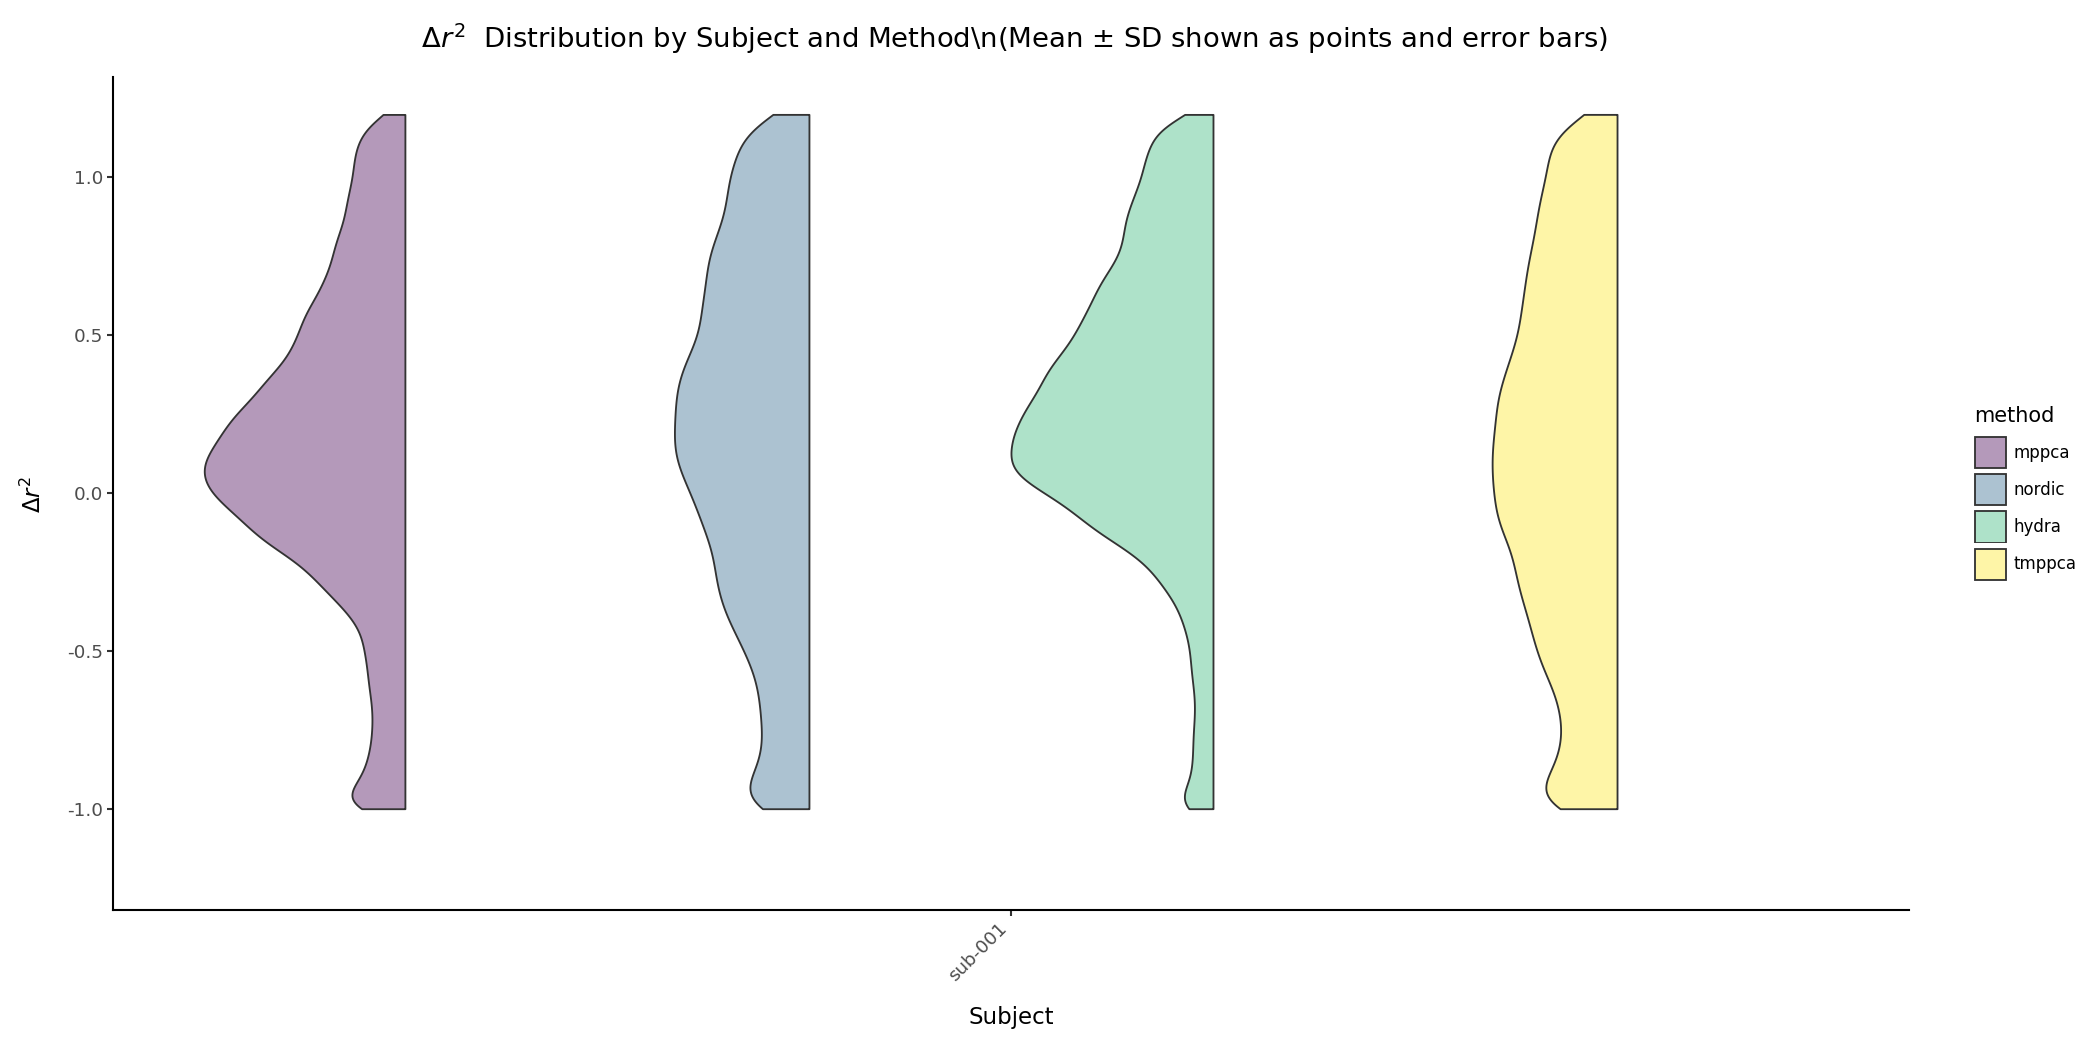
\includegraphics[width=7cm]{images/halfviolin_r2spc_across_subjects_maskedHR.png} \\
    \end{tabular}
    \caption[Distribution of functional connectivity reliability changes per dataset ($r^2$)]{Histograms of $\Delta r^2$ (relative change with respect to no denoising (vanilla)).}
\label{fig:reliabilityFCspc}
\end{figure}

Figure~\ref{fig:intereliability} summarizes the FC analysis on independently denoised halves. For each method, the left side of the violin plot (green) shows the distribution of $r^2$ obtained when each half is denoised independently (“independent denoising”). The right side shows the distribution when the full time series is denoised jointly (“joint denoising”). The two distributions overlap substantially, but joint denoising yields a slight shift toward higher $r^2$ values—as expected, because noise estimates are derived from the same data used for reliability calculation. Importantly, estimating the noise floor on independent halves yields comparable reliability scores, indicating that the denoising strategies robustly remove non‑signal components and identify them consistently across independent data segments.

Of particular note, TMPPCA shows the smallest overlap between independent and joint denoising. This is consistent with TMPPCA leveraging temporal redundancy: larger datasets improve noise‑estimation precision. 

\begin{figure}[tb!]
    \centering
    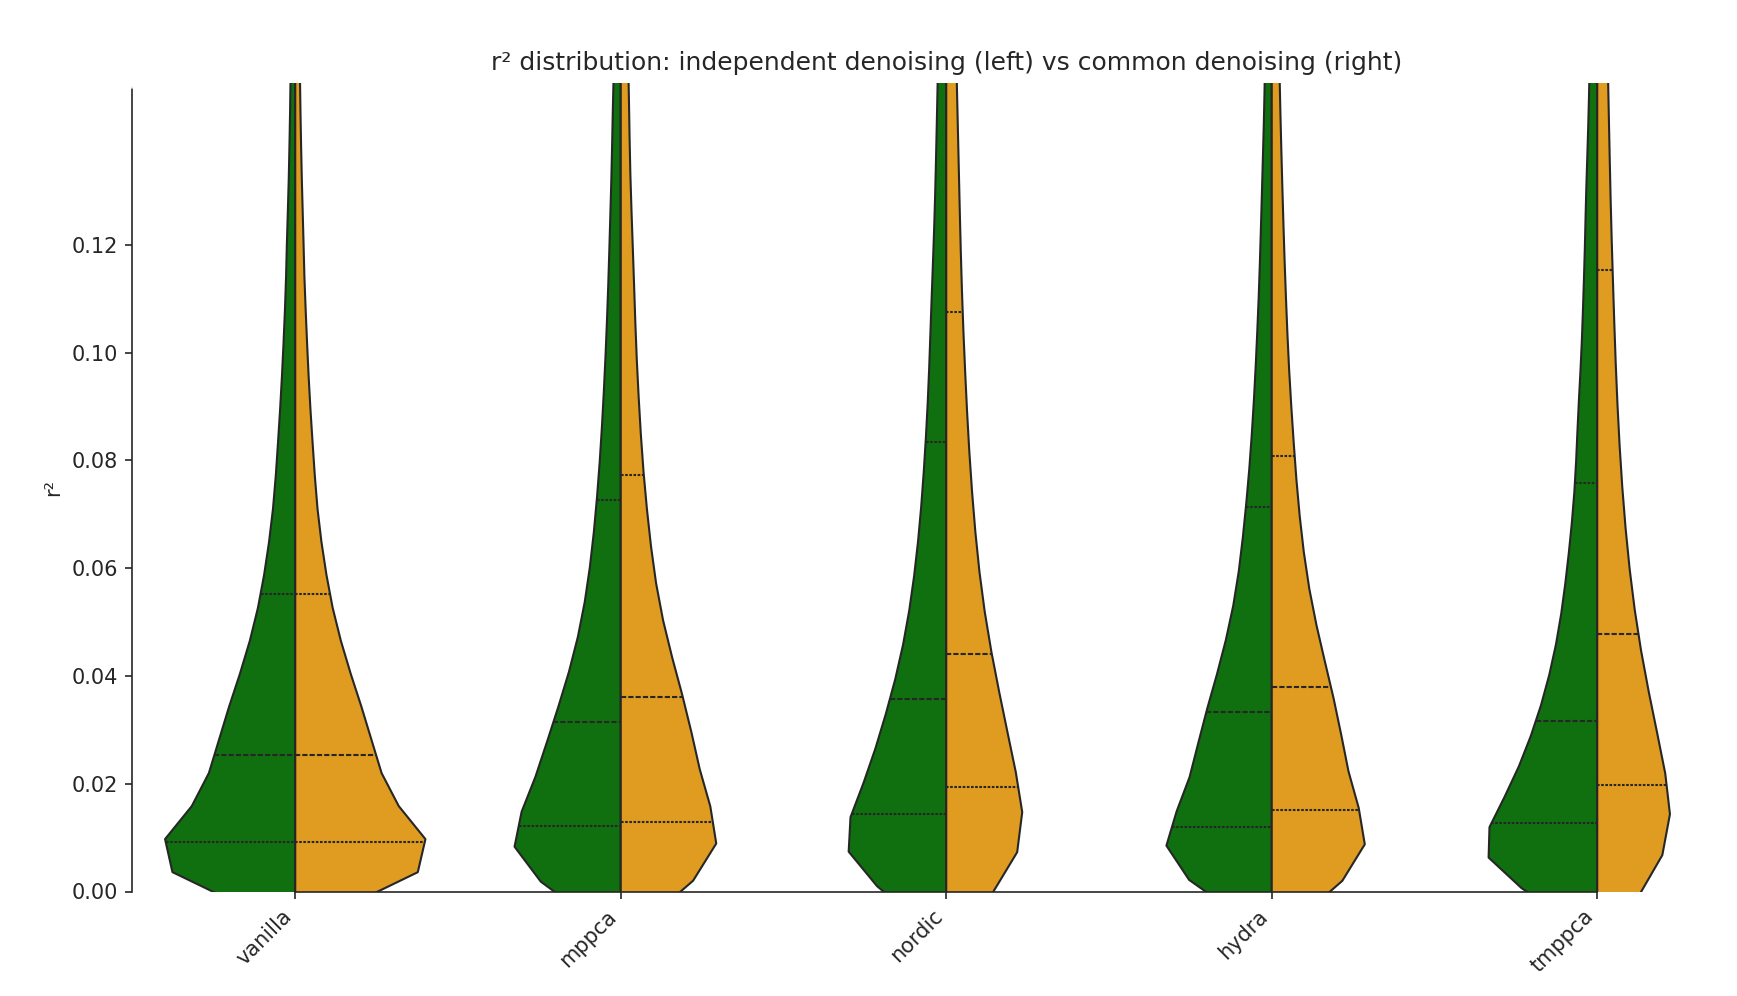
\includegraphics[width=11cm]{images/reliability_betweenruns.png}
    \caption[Comparison of reliability estimates obtained from independently denoised data halves at high spatial resolution (1.5 mm isotropic)]{Comparison of reliability ($r^2$) from independently denoised data halves (left) vs. jointly denoised full time series (right) at 1.5 mm. Reliability is highly consistent across methods, as evidenced by the close correspondence between halves and joint estimates in each violin plot.}
    \label{fig:intereliability}
\end{figure}


\section{Discussion}

\begin{figure}
    \centering
    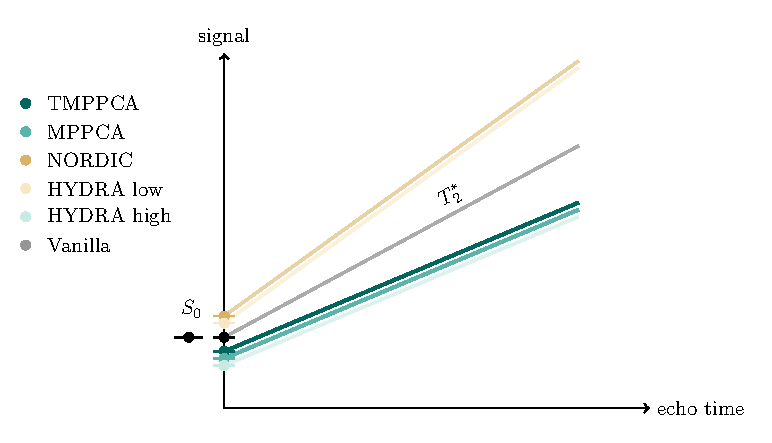
\includegraphics[width=9cm]{images/thermal_signal_ME.pdf}
    \caption[Multi-echo signal model fitting per denoising method]{Illustration of multi-echo signal fitting per denoising method. The intercept corresponds to $S_0$ and the slope to $T_2^*$.}
    \label{fig:thermal_signal_ME}
\end{figure}

Multi-echo fMRI enhances signal quality by linearly combining information across multiple echoes, thereby increasing sensitivity to BOLD-related neurophysiological changes \citep{poser2006bold, kundu2017multi}. The ongoing trend toward higher spatial resolution, achieved via smaller voxels and faster sequences, necessitates effective strategies for maintaining signal quality \citep{feinbergRapidDevelopmentHigh2012, aja-fernandezNoiseEstimationParallel2014, pruessmann1999sense}. Integrating multi-echo acquisition with thermal denoising algorithms thus represents a particularly valuable approach for high resolution applications.

Consistent with previous single‑echo findings, random matrix theory‑based denoising methods improved overall signal quality, as reflected in the tSNR distributions in all datasets (Fig.~\ref{fig:tsnrDistribution}) \citep{veraart2016denoising, zhu2022denoise, nigiImprovedNoiseReduction2023a, dowdle2023evaluating}. Among the evaluated methods, TMPPCA consistently yielded the most substantial improvements in tSNR.

A core premise of multi‑echo fMRI is that echo combination depends on accurate, data‑driven $T_2^*$ and $S_0$ estimates to maximize BOLD sensitivity (Sec.~\ref{sec:MEfMRI}) \citep{poser2006bold}. If thermal denoising altered the signal of interest, systematic changes in these parameters would be expected \citep{kundu2017multi, kundu2012differentiating}, which is exactly what we observed for all denoising methods, but only in low‑quality signal regions (Fig.~\ref{fig:thermal_signal_ME}). Two patterns emerged: MPPCA, TMPPCA, and HYDRA in the high‑resolution dataset slightly reduced both the intercept ($S_0$) and slope ($\overline{R_2^*}$), whereas NORDIC and HYDRA in the low‑resolution datasets slightly increased both. The latter likely reflects signal leakage from high‑ to low‑SNR regions, artificially inflating the signal, consistent with prior reports for MPPCA‑based methods \citep{fernandesMPPCADenoisingFMRI2023a, zhu2022denoise, comby2023denoising}. 

Although TMPPCA provided the largest tSNR gains, its $T_2^$ and $S_0$ estimates remained close to, but slightly below, those from undenoised data, similar to MPPCA, likely because denoising was applied to the magnitude data. This indicates that these methods systematically remove variance.

Running NORDIC independently across echoes denoises the complex signal and better respects thermal noise assumptions \citep{gudbjartssonRicianDistributionNoisy1995c, vizioli2021lowering} than MPPCA or TMPPCA. However, it slightly biases signal estimates in regions with dropout, field inhomogeneities, or high g‑factor penalties—such as deep and subcortical structures, orbitofrontal, anterior frontal, and inferior temporal lobes—due to signal leakage \citep{kay2022riskL, fernandesMPPCADenoisingFMRI2023a}. We hypothesized that spatially concatenating echoes before applying NORDIC would better exploit spatial redundancy and further improve performance, but this was not the case.


Another key question was how thermal denoising affects the detectability of BOLD‑related signal changes over time. Because these changes are small in magnitude, improving sensitivity is substantial for fMRI research. All thermal denoising strategies increased the proportion of plausible $\Delta R_2^$ estimates, especially with TMPPCA. This demonstrates that the variance removed leads to more confident estimates of $\Delta R_2^$, which in turn is an indirect measure of MRI sensitivity.

We next assessed the feasibility of the denoising strategies by examining their impact on functional connectivity (FC) analysis. We hypothesized that thermal denoising would enhance temporal signal stability and thereby strengthen FC estimates for signals of interest. Consistent with the physiological‑thermal noise trade‑off (Sec.~\ref{sec:noiseMRI}), FC reliability increased at lower spatial resolutions (2.4 and 2 mm), likely because both physiological and thermal noise compromise signal integrity at this resolution. This improvement can be attributed to higher SNR regimes, together with the reduced relative impact of motion on voxel‑wise identifiability: a given displacement (e.g., 2 mm) corresponds to approximately one voxel at 2 or 2.4 mm resolution, whereas the same displacement approaches two voxels at 1.5 mm resolution\citep{bodurkaMappingMRIVoxel2007, satterthwaite2019motion}.

For the lower spatial resolution datasets, reliability metrics increased following thermal denoising.  In contrast, for the high‑resolution dataset, all denoising methods led to an increase in reliability metrics for some voxels but a decrease in others. Increases in $r^2$ values originated in regions with higher baseline signal (i.e., those closest to the receive coils) and then extended into more distal gray matter areas \citep{wald2017impacting, pohmannSignalnoiseRatioField2024}. With TMPPCA, the enhancement propagated even further, reaching distant regions such as the frontal lobe in the low resolution datasets, thus while getting an increase in some voxels at high resolution, it also showed some decrease. When comparing each denoising strategy against undenoised data, TMPPCA consistently yielded the largest improvements across all datasets, providing strong evidence for its efficacy and robustness. NORDIC systematically ranked second.

Finally, we evaluated the stability of denoising procedures using the high‑resolution dataset. If noise estimation and removal are truly data‑driven and do not introduce substantial artifacts, then voxelwise FC matrices computed separately for each half of the data, and their associated between‑halves reliability indices, should be highly similar whether this FC matrices comes from a independent or a joint denoising \citep{lynchRapidPrecisionFunctional2020}. Our results indicate that reliability values remain notably stable even when each half is denoised independently, and this pattern is consistent across denoising strategies.

\section{Conclusions}

We investigated the effect of thermal denoising on multi‑echo signal quality and sensitivity. For signal quality, thermal denoising increased temporal signal‑to‑noise ratio (tSNR) in both low‑ and high‑resolution acquisitions. In low‑resolution data, TMPPCA consistently outperformed other methods: it achieved the highest tSNR, improved multi‑echo parameter estimates, and enhanced reliability, with benefits extending to brain regions distant from the receive coils. In high‑resolution data, TMPPCA again yielded the best tSNR and multi‑echo estimates; however, its reliability gains were not uniform, with some voxels showing lower reliability compared to no denoising.

Given the central role of functional connectivity analyses in brain research, our results indicate that TMPPCA is the most effective strategy for improving signal quality and sensitivity in high‑resolution acquisitions, while preserving the integrity of multi‑echo combination parameters.

